%!TEX output_directory = ../bin

\documentclass[a4paper, 92pt, twoside,openright]{report}
\usepackage{multirow}
\usepackage{tabulary}
\usepackage{tabularx}
\usepackage{pdfpages}
\usepackage{amsmath,amssymb,stmaryrd}   
\usepackage{anyfontsize}
\usepackage{multicol}
\usepackage{booktabs}
% \usepackage{algorithm}
\usepackage{algorithmic}
\usepackage{listings}
\usepackage{wrapfig}
% \usepackage{placeins}
\usepackage{float}
\usepackage{algorithm2e}
\usepackage{longtable}

\usepackage{etoolbox}
\usepackage[utf8]{inputenc}
\usepackage[T1]{fontenc}
\usepackage{adjustbox}
\usepackage{siunitx}
\usepackage{enumitem}
\usepackage{subcaption}
\usepackage{url}
\usepackage{lscape,lipsum}
\usepackage{everypage}
\usepackage{eurosym} % euro s


\usepackage{bytefield}
  \newcommand{\y}[2]{\bitbox{#1}{#2}}


\usepackage{xparse}

\ExplSyntaxOn
\NewDocumentCommand{\xinput}{m}{%
  \azimut_xinput:n { #1 }
}

\ior_new:N \g_azimut_xinput_stream

\cs_new_protected:Nn \azimut_xinput:n
 {
  \ior_open:Nn \g_azimut_xinput_stream { "|ls ~ #1" }
  \ior_map_inline:Nn \g_azimut_xinput_stream { \file_input:n { \tl_trim_spaces:n {##1} } }
 }
\ExplSyntaxOff


\input{setup/setup_rgb}

\def\blue#1{\textcolor{beamer@blendedblue}{#1}}
\def\violet#1{\textcolor{violet}{#1}}
\def\yellow#1{\textcolor{yellow}{#1}}
\def\red#1{\textcolor{red}{#1}}
\def\green#1{\textcolor{green}{#1}}
\def\black#1{\textcolor{black}{#1}}

%\renewcommand{\arraystretch}{1.5}


\usepackage{array}
\usepackage{ragged2e}
% \usepackage{array}
% \newcolumntype{lj}[1]{>{\raggedright\let\newline\\\arraybackslash\hspace{0pt}}m{#1}}
% \newcolumntype{j}[1]{>{\centering\let\newline\\\arraybackslash\hspace{0pt}}m{#1}}
% \newcolumntype{rj}[1]{>{\raggedleft\let\newline\\\arraybackslash\hspace{0pt}}m{#1}}
\newcolumntype{P}{@{\hspace{1pt}}>{\RaggedLeft}m{0.22cm}}



\newcommand\Mark[1]{\textsuperscript#1}
\def\res{../res}
\def\plot{setup/plot}

%\begin{figure}
%\begin{center}
%\begin{tabular}{cc}
%\resizebox{60mm}{!}{\includegraphics{test1.eps}} &
%\resizebox{60mm}{!}{\includegraphics{test2.eps}} \\
%\resizebox{60mm}{!}{\includegraphics{test3.eps}} &
%\resizebox{60mm}{!}{\includegraphics{test4.eps}} \\
%\end{tabular}
%\caption{This is sample figures.}
%\label{test4}
%\end{center}
%\end{figure}

\usepackage{pgfplots}
\usepackage{filecontents}
\pgfplotsset{compat=newest}
\usepgfplotslibrary{patchplots}
\usepackage{tikz}
\usepackage{pgfplots}
\pgfplotsset{
	table/search path={\res/data/},
}
\usetikzlibrary{backgrounds}
\usetikzlibrary{graphs, graphs.standard, graphdrawing}

\newcommand{\shaded}[1]{\textcolor{gray!30}{#1}}
\usepackage{pifont}
	\newcommand{\ok}{\textcolor{green}{\ding{51}}}
	\newcommand{\ko}{\textcolor{red}{\ding{55}}}

\newcolumntype{?}{!{\vrule width 1pt}}

\newcommand\addchapter[1]{
	\addcontentsline{toc}{chapter}{#1}
}

\newcommand\Printbibliography[9]{
% \addcontentsline{toc}{chapter}{Bibliography}
\ifthenelse{\equal{\thepart}{0}}{}{\printbibheading}
\epigraph{"A quote in a speech, article or book is like a gun in the hands of a soldier. It speaks with authority."}{}
	\aghiles{#1}
	\aghiles{#2}
	\aghiles{#3}
	\aghiles{#4}
	\aghiles{#5}
	\aghiles{#6}
	\aghiles{#7}
	\aghiles{#8}
	\aghiles{#9}
	\printbibliography[heading=subbibliography,%
	notkeyword={#1},%
	notkeyword={#2},%
	notkeyword={#3},%
	notkeyword={#4},%
	notkeyword={#5},%
	notkeyword={#6},%
	notkeyword={#7},%
	notkeyword={#8},%
	notkeyword={#9},% 
	title=Others]
}


\usepackage{hyperref}
\hypersetup{
%	pdftex,
%	pdfpagemode=FullScreen,
    pdftoolbar=true,        % show Acrobat’s toolbar?
%    pdfborder={0 0 0},
    pdfmenubar=true,        % show Acrobat’s menu?
    pdffitwindow=true,     % window fit to page when opened
    pdfstartview={FitH},    % fits the width of the page to the window
%    pdftitle={title},    % title
%    pdfauthor={Salvatore Mazzarino},     % author
%    pdfsubject={Subject},   % subject of the document
%    pdfcreator={Salvatore Mazzarino},   % creator of the document
%    pdfproducer={Salvatore Mazzarino}, % producer of the document
%    pdfkeywords={Green Networking} {Mobile Cloud} {Network Coding} {Energy}, % list of keywords
    pdfnewwindow=true,      % links in new window
    colorlinks=true,       % false: boxed links; true: colored links
    linkcolor=beamer@blendedblue,          % color of internal links (change box color with linkbordercolor)
    citecolor=beamer@blendedblue,        % color of links to bibliography
    filecolor=beamer@blendedblue,      % color of file links
    urlcolor=beamer@blendedblue           % color of external links
}
    
%    hyperfootnotes=true,
%	breaklinks=true,
%	bookmarksopen=true,
%	backref=page

% sudo apt-get install biber
\usepackage[sorting=none,backref=false,backend=biber, doi=false,url=false,isbn=false, style=numeric]{biblatex}%sorting=nyt, sorting=rasha
%\usepackage[sorting=none,backref=true,backend=biber,sorting=rasha, doi=false,url=false,isbn=false, citetracker,pagetracker=page]{biblatex}%sorting=nyt
	%\setbeamertemplate{bibliography item}{\insertbiblabel}
	%Comme back from citation backref=true
	\addbibresource{/home/aghiles/Aghiles/Redaction/lib/iot.bib}%
	\addbibresource{/home/aghiles/Aghiles/Redaction/lib/iotbis.bib}%
	\addbibresource{/home/aghiles/Aghiles/Redaction/lib/privacy.bib}%
	% \addbibresource{/home/aghiles/Aghiles/Redaction/lib/privacybis.bib}
	\def\bibfont{\small}
	\DefineBibliographyStrings{english}{%
		backrefpage = {p.},% originally "cited on page"
		backrefpages = {p.},% originally "cited on pages"
	}
	% Define new format that applies a hypertext reference
	\DeclareFieldFormat{linked}{%
		\ifboolexpr{ test {\ifhyperref} and not test {\ifentrytype{online}}}{
			\iffieldundef{file}{
				\iffieldundef{url}{#1}{\href{run:\thefield{url}}{#1}}
			}{%
				\StrCount{\thefield{file}}{:}[\nbmatch]%
				\StrCut[\nbmatch]{\thefield{file}}{:}\strfirst\strsecond%
				\StrCount{\strfirst}{:}[\nbmatch]%
				\StrCut[\nbmatch]{\strfirst}{:}\strfirst\strsecond%
				\href[pdfnewwindow]{run:\strsecond}{#1}
%				\href{run:\thefield{file}}{#1}
			}
		}{#1}
	}
	% Based on generic definition from biblatex.def
	\renewbibmacro{title}{%
		\ifboolexpr{ test {\iffieldundef{title}} }{}{
			\printtext[title]{
				\printtext[linked]{\printfield[titlecase]{title}}
			}
			\newunit
		}%
		\printfield{titleaddon}%
	}
	% %
	% \DeclareSourcemap{
	%   \maps[datatype=bibtex]{
	%     \map[overwrite]{
	%        \step[fieldsource=groups,]
	%        \step[fieldset=keywords, fieldvalue={,}, append]
	%        \step[fieldset=keywords, origfieldval, append]
	%     }
	%   }
	% }

	\DeclareSourcemap{
	\maps[datatype=bibtex]{
			\map[overwrite=true]{
		       \step[fieldsource=groups,]
		       \step[fieldset=keywords, fieldvalue={,}, append]
		       \step[fieldset=keywords, origfieldval, append]
			}
		}
	}
	%
%	\DeclareSortingTemplate{rasha}{
%		\sort[direction=ascending]{
%			\field{year}}
%		\sort{\field{presort}}
%	}
	
	\newcommand{\aghiles}[1]{\printbibliography[heading=subbibliography, keyword={#1}, title={#1}]}

%Todo
\newcounter{todo}
\usepackage{tcolorbox}
	\newtcbox{\mytodobox}{colback=white,colframe=white!75!white}
\newcommand\todo[1]{
	\refstepcounter{todo}
	\mytodobox{\hypertarget{todo\thetodo}{#1}}
	\addcontentsline{tod}{subsection}{\protect\hyperlink{todo\thetodo}{\thetodo~#1}\par} }
\makeatletter
\newcommand\listoftodos{
	\@starttoc{tod}}
\makeatother

\usepackage{graphicx}
	\graphicspath{ {\res/} {\res/diagram/} {\res/icon/} {\res/plot/} {\res/stat/} {\res/tikz/} {\res/tmp/} {../plot/} }

\newcommand{\towFigure}[5]{
	\medskip
	\begin{figure}
		\includegraphics[width=#1\columnwidth]{#2} \\
		\includegraphics[width=#1\columnwidth]{#3}
		\caption{#5.}\label{fig:#4}
	\end{figure}
	\medskip
}

\newcommand{\towFigureT}[5]{
	\medskip
	\begin{figure}
		\includegraphics[width=#1\columnwidth]{#2} \\
		\includegraphics[width=#1\columnwidth]{#3}
		\caption*{\blue{Figure} \ref{fig:#4}: #5.}
%		\caption{#5.}\label{fig:#4}
	\end{figure}
	\medskip
}

\newcommand{\Figure}[4]{
	\begin{figure}[#1]
	\centering
	\includegraphics[width=#2\columnwidth]{#3}
	\caption{#4.}\label{fig:#3}
	\end{figure}
}

\newcommand{\Tickz}[4]{
	\medskip
	\begin{figure}[#1]
			\centering
			\begin{tikzpicture}[scale=#2,line width=1pt]
				\input{\plot/#3}
			\end{tikzpicture}
	\caption{#4.}\label{fig:#3}
	\end{figure}
	\medskip
}

\newcommand{\FigureS}[4]{
	\medskip
	\begin{figure}[#1]
	\centering
	\includegraphics[width=#2\columnwidth]{#3}
	\caption*{\blue{Figure \ref{fig:#3}:} #4.}
	\end{figure}
	\medskip
}

\newcommand{\FigureT}[3]{
	\medskip
	\begin{figure}[#1]
	\centering
	\includegraphics[width=#2\columnwidth]{#3}
	\end{figure}
	\medskip
}

\usepackage{subcaption}
	\captionsetup{justification=centering}
	\captionsetup[table]{skip=10pt}
%	\captionsetup{labelfont=it,textfont={bf,it},justification=centering}
	
\renewcommand{\thesubfigure}{\alph{subfigure}}
\renewcommand{\thefigure}{\arabic{figure}}

\newcommand{\FigureH}[8]{
%	\medskip
	\begin{figure}
		\centering
		\begin{subfigure}[#1]{#2\columnwidth}
			\centering
			\includegraphics[width=\columnwidth]{#3}
			\caption{#4.}\label{fig:#3}
		\end{subfigure}
		~ % \quad, \qquad, \hfill
		\begin{subfigure}[#1]{#2\columnwidth}
			\centering
			\includegraphics[width=\columnwidth]{#5}
			\caption{#6.}\label{fig:#5}
		\end{subfigure}
		
		\caption{#8.}\label{fig:#7}
	\end{figure}
%	\medskip
}

\newcommand{\FigureV}[8]{
%	\medskip
	\begin{figure}
		\centering
		\begin{subfigure}[#1]{\columnwidth}
			\centering
			\includegraphics[width=#2\columnwidth]{#3}
			\caption{#4.}\label{fig:#3}
		\end{subfigure}
		~ % \quad, \qquad, \hfill
		\begin{subfigure}[#1]{\columnwidth}
			\centering
			\includegraphics[width=#2\columnwidth]{#5}
			\caption{#6.}\label{fig:#5}
		\end{subfigure}
		
		\caption{#8.}\label{fig:#7}
	\end{figure}
%	\medskip
}

\newcommand{\TickzH}[9]{
%	\medskip
	\begin{figure}
	\begin{center}
		\begin{subfigure}[#1]{#2\columnwidth}
			\centering
			\begin{tikzpicture}[scale=#9,line width=1pt]
				\input{\plot/#3}
			\end{tikzpicture}
			\caption{#4.}\label{fig:#3}
		\end{subfigure}
		~ % \quad, \qquad, \hfill
		\begin{subfigure}[#1]{#2\columnwidth}
			\centering
			\begin{tikzpicture}[scale=#9,line width=1pt]
				\input{\plot/#5}
			\end{tikzpicture}
			\caption{#6.}\label{fig:#5}
		\end{subfigure}
		\caption{#8.}\label{fig:#7}
	\end{center}
	\end{figure}
%	\medskip
}

\newcommand{\TickzV}[8]{
%	\medskip
	\begin{figure}
		\centering
		\begin{subfigure}[#1]{\columnwidth}
			\centering
			\begin{tikzpicture}[scale=#2,line width=1pt]
				\input{\plot/#3}
			\end{tikzpicture}
			\caption{#4.}\label{fig:#3}
		\end{subfigure}
		~ % \quad, \qquad, \hfill
		\begin{subfigure}[#1]{\columnwidth}
			\centering
			\begin{tikzpicture}[scale=#2,line width=1pt]
				\input{\plot/#5}
			\end{tikzpicture}
			\caption{#6.}\label{fig:#5}
		\end{subfigure}
		
		\caption{#8.}\label{fig:#7}
	\end{figure}
%	\medskip
}


\newcommand{\Equation}[2]{
	\begin{equation}\label{eq:#1}
		#2
	\end{equation}
}

\newcommand{\EquationT}[2]{
	\begin{equation*}\tag{\ref{eq:#1}}
		#2
	\end{equation*}
}

\newcommand{\EquationS}[1]{
	\begin{equation*}
		#1
	\end{equation*}
}

% \newcommand{\Center}[1]{
% 	\begin{center}
% 		#1
% 	\end{center}
% }

\newcommand{\Itemize}[1]{
	\begin{itemize}
		#1
		\bigskip
	\end{itemize}
	\medskip
}

\newcommand{\Enumerate}[1]{
	\begin{enumerate}
		#1
		\bigskip
	\end{enumerate}
	\medskip
}

\newcommand{\Columns}[4]{
	\begin{columns}
		\begin{column}{#1\textwidth}
		#3
		\end{column}
		\begin{column}{#2\textwidth}
		#4
		\end{column}
	\end{columns}
}

\newcommand{\Table}[4]{
	\begin{table}[h!]
		\centering
		\begin{tabulary}{\textwidth}{#1}
			#4
		\end{tabulary}
		\caption{\label{table:#2} #3.}
	\end{table}
}

\newcommand{\TableT}[4]{
	\begin{table}[h!]
	\centering
		\begin{tabular}{#1}
			#4
		\end{tabular}
		\caption*{\blue{Table \ref{table:#2}:~} #3.}
	\end{table}
}

\usepackage{bytefield}


% \usepackage{enumitem}
% \setlistdepth{9}
% \setlist[itemize,1]{label=\violet{\ding{224}}}
% \setlist[itemize,2]{label=\violet{\ding{223}}}
% \setlist[itemize,3]{label=\violet{\ding{84}}}
% \setlist[itemize,4]{label=\violet{\Rightarrow}}
% \setlist[itemize,5]{label=\violet{$\gg$}}
% \setlist[itemize,6]{label=\violet{$\leadsto$}}


% % \setlist[itemize,1]{label=\violet{$\bullet$}}
% % \setlist[itemize,2]{label=\violet{$\bullet$}}
% % \setlist[itemize,3]{label=\violet{$\bullet$}}
% % \setlist[itemize,4]{label=\violet{$\bullet$}}
% % \setlist[itemize,5]{label=\violet{$\bullet$}}
% % \setlist[itemize,6]{label=\violet{$\bullet$}}
% \setlist[itemize,7]{label=\violet{$\bullet$}}
% \setlist[itemize,8]{label=\violet{$\bullet$}}
% \setlist[itemize,9]{label=\violet{$\bullet$}}
% \renewlist{itemize}{itemize}{9}

\usepackage{enumitem}
\setlistdepth{9}
\setlist[itemize,1]{label=\violet{\ding{224}}}
\setlist[itemize,2]{label=\violet{\ding{223}}}
\setlist[itemize,3]{label=\violet{\ding{84}}}
\setlist[itemize,4]{label=\violet{\Rightarrow}}
\setlist[itemize,5]{label=\violet{$\gg$}}
\setlist[itemize,6]{label=\violet{$\leadsto$}}
\setlist[itemize,7]{label=\violet{$\bullet$}}
\setlist[itemize,8]{label=\violet{$\bullet$}}
\setlist[itemize,9]{label=\violet{$\bullet$}}
\renewlist{itemize}{itemize}{9}


\AtBeginDocument{% ...if you're using hyperref
  \let\oldlabel\label% Copy original version of \label
  \let\oldref\ref% Copy original version of \ref
}

\newcommand{\addlabelprefix}[1]{%
  \renewcommand{\label}[1]{\oldlabel{#1-##1}}% Update \label
  \renewcommand{\ref}[1]{\oldref{#1-##1}}% Update \ref
}
\newcommand{\removelabelprefix}{%
  \renewcommand{\label}{\oldlabel}% Restore \label
  \renewcommand{\ref}{\oldref}% Restore \ref
}

% Accronime et abriviation
\usepackage{acro}
%first-long-format=\itshape
\acsetup{hyperref=true}
	\newcommand{\addac}[2]{
		\DeclareAcronym{#1}{
			short = \ensuremath{#1},
			long  = {#2},
			sort  = {#1},
			class = nomencl
		}
	}
	\newcommand{\addab}[2]{
		\DeclareAcronym{#1}{
			short = {#1} ,
			long  = {#2},
			sort  = {#1},
			class = abbrev
		}
	}
	
%Abreviation

\addab{CSS}{Chirp Spread Spectrum (Proprietary)}
\addab{PCB}{Printed Circuit Board}
\addab{ny}{New York}
\addab{ACL}{Access Control List}
\addab{FHSS}{Frequency Hopping Spread Spectrum}
\addac{Sen}{Sensitivity}


%% Nomenclature

\addac{NY}{New York}
\addac{MCU}{Micro Controller Unit}
\addac{LoRa}{Long Range}
\addac{RSSI}{Received Signal Strength Indication}
\addac{CR}{Coding Rate}


\addac{PDR}{Packet delivery ratio}
\addac{SF}{Spreading Factor}
\addac{BS}{Base Station}
\addac{FEC}{Forward error correction}
\addac{LS}{Link Symmetry}

\addac{BER}{Bit Error Rate}
\addac{PER}{Packet Error Rate}
\addac{PRR}{Packet Reception Rate}

\addac{RS}{Receiver Sensitivity}

\addac{AT}{Air Time}
\addac{PLR}{Packet loss rate}
\addac{BR}{Bit Rate}
\addac{DR}{Data Rate}
\addac{ADR}{Adaptive Data Rate}
\addac{SR}{Symbol Rate}
\addac{SNR}{Signal Noise Rate}
\addac{BW}{Bandwidth}
\addac{PL}{Payload length}
\addac{CF}{Carrier Frequency}

\addac{MSE}{Mean Squared Error}
\addac{RMSE}{Root Mean Squared Error}
\addac{MAE}{Mean Absolute Error}
\addac{ROC}{Receiver Operating Characteristic}
\addac{TPR}{True Positive Rate}
\addac{FPR}{False Positive Rate}
\addac{NDCG}{Normalized Discounted Cumulative Gain}


\addac{PS}{Payload size}
\addac{Tx}{Transmission Energy}
\addac{ToA}{Time on Air}
\addac{RTT}{Round time trip}
\addac{SINR}{Signal-to-interference \& noise ratio}
\addac{SIR}{Signal-to-Interference Ratio} 

\addac{TC}{Traffic congestion}
\addac{DC}{Duty cycle}
\addac{Mob}{Mobility}
\addac{CCI}{Co-channel Interference}

\addac{SL}{Sleep time}
\addac{Jit}{Jitter}

\addac{SC}{Service Cost}
\addac{Th}{Throughput}



% \usepackage[titles]{tocloft}
% \newlistentry[subparagraph]{subsubparagraph}{toc}{5}

%\newcounter{subsubparagraph}

% \titleclass{\subparagraph}{straight}[\paragraph]
% \titleclass{\subsubparagraph}{straight}[\subparagraph]

% \renewcommand{\thesubparagraph}{\arabic{paragraph}.\arabic{subparagraph})}
% \renewcommand{\thesubsubparagraph}{\Alph{subsubparagraph})}

% \titleformat*{\subparagraph}{\normalfont\color{violet}}
% \titleformat{\subsubparagraph}[runin]{\normalfont\normalsize\bfseries}{\thesubsubparagraph}{1em}{}
% \titleformat*{\subsubparagraph}{\normalfont\color{violet}}


\newcommand{\compresslist}{%
    \setlength{\itemsep}{0pt}%
    \setlength{\parskip}{1pt}%
    \setlength{\parsep}{0pt}%
}


% \usepackage{lmodern}
% 	\selectcolormodel{cmyk}


\def\d{$\downarrow$}
\def\u{$\uparrow$}

%\usepackage[a4paper]{geometry}

\usepackage[top=2.5cm, bottom=2cm, left=3cm, right=2.5cm, headheight=15pt]{geometry}

\def\titlepage{
	\newpage
	\centering
	\linespread{1}
	\normalsize
	\vbox to \vsize\bgroup\vbox to 9in\bgroup
}
\def\endtitlepage{
	\par
	\kern 0pt
	\egroup
	\vss
	\egroup
	\cleardoublepage
}

\pagestyle{empty}
\makeatletter
	\def\@ecole{école}
	\newcommand{\ecole}[1]{\def\@ecole{#1}}

	\def\@specialite{Spécialité}
	\newcommand{\specialite}[1]{\def\@specialite{#1}}

	\def\@directeur{directeur}
	\newcommand{\directeur}[1]{\def\@directeur{#1}}

	\def\@encadrant{encadrant}
	\newcommand{\encadrant}[1]{\def\@encadrant{#1}}
	
	\def\@jurya{}{}{}
	\newcommand{\jurya}[3]{\def\@jurya{#1,	& #2	& #3\\}}
	
	\def\@juryb{}{}{}
	\newcommand{\juryb}[3]{\def\@juryb{#1,	& #2	& #3\\}}
	
	\def\@juryc{}{}{}
	\newcommand{\juryc}[3]{\def\@juryc{#1,	& #2	& #3\\}}
	
	\def\@juryd{}{}{}
	\newcommand{\juryd}[3]{\def\@juryd{#1,	& #2	& #3\\}}
	
	\def\@jurye{}{}{}
	\newcommand{\jurye}[3]{\def\@jurye{#1,	& #2	& #3\\}}
	
	\def\@juryf{}{}{}
	\newcommand{\juryf}[3]{\def\@juryf{#1,	& #2	& #3\\}}
	
	\def\@juryg{}{}{}
	\newcommand{\juryg}[3]{\def\@juryg{#1,	& #2	& #3\\}}
	
	\def\@juryh{}{}{}
	\newcommand{\juryh}[3]{\def\@juryh{#1,	& #2	& #3\\}}
	
	\def\@juryi{}{}{}
	\newcommand{\juryi}[3]{\def\@juryi{#1,	& #2	& #3\\}}
\makeatother

\newcommand\BackgroundPic{%
	\put(0,0){%
		\parbox[b][\paperheight]{\paperwidth}{%
			\includegraphics[height=0.45\paperheight]{Bordure.png}%
			\vfill
		}
	}
}
\newcommand\EtiquetteThese{%
	\put(0,0){%
		\parbox[t][\paperheight]{\paperwidth}{%
			\hfill
			\colorbox{blue}{
				\begin{minipage}[b]{3em}
					\centering\Huge\textcolor{white}{T\\H\\E\\S\\E\\}
					\vspace{0.2cm}
				\end{minipage}
			}
		}
	}
}

\makeatletter
\newcommand{\firstpage}{
	\newgeometry{top=2.5cm, bottom=2cm, left=2cm, right=1cm}
	\AddToShipoutPicture*{\BackgroundPic}
	\AddToShipoutPicture*{\EtiquetteThese}
	\begin{titlepage}
		\centering
			
\includegraphics[width=0.2\textwidth]{upmc}
			\hfill
			
\includegraphics[width=0.2\textwidth]{sorbonne}\\
		\vspace{1cm}
			{\Large \'{E}cole doctorale 364 : Sciences Fondamentales et Appliquées}\\
		\vspace{1cm}
			{\huge {\bfseries Doctorat ParisTech}\\
		\vspace{0.5cm}
			TH\`{E}SE}\\
		\vspace{1cm}
			{\bfseries pour obtenir le grade de docteur délivré par}\\
		\vspace{1cm}
			{\huge\bfseries \@ecole}\\
		\vspace{0.5cm}
			{\Large{\bfseries Spécialité doctorale ``\@specialite''}}\\
		\vspace{2cm}
			\textit{présentée et soutenue publiquement par}\\
		\vspace{0.5cm}
			{\Large {\bfseries \@author}} \\
		\vspace{0.5cm}
			le \@date \\
		\vfill
			{\LARGE \color[rgb]{0,0,1} \bfseries{\@title}} \\
		\vfill
			Directeur de thèse : {\bfseries \@directeur}\\
			Co-encadrant de thèse : {\bfseries \@encadrant}\\
		\vfill
		\begin{tabular}{>{\bfseries}llr}
			\large Jury\\
			\@jurya
			\@juryb
			\@juryc
			\@juryd
			\@jurye
			\@juryf
			\@juryg
			\@juryh
			\@juryi
		\end{tabular}
		\vfill
	\end{titlepage}
	\restoregeometry
}
\makeatother

%%%%%%%%%%%
% Preface %
%%%%%%%%%%%

\def\abstract{
	\begin{center}{
		\large\bf Abstract}
	\end{center}
	\small
	%\def\baselinestretch{1.5}
	\linespread{1.5}
	\normalsize
}

\def\endabstract{
	\par
}

\newenvironment{acknowledgements}{
	\cleardoublepage
	\begin{center}{
		\large \bf Acknowledgements}
	\end{center}
	\small
	\linespread{1.5}
	\normalsize
}{\cleardoublepage}

\def\endacknowledgements{
	\par
}

\newenvironment{dedication}{
	\cleardoublepage
	\begin{center}{
		\large \bf Dedication}
	\end{center}
	\small
	\linespread{1.5}
	\normalsize
}{\cleardoublepage}

\def\enddedication{
	\par
}

\usepackage{setspace}
\def\preface{
		\pagenumbering{roman}
		\pagestyle{plain}
%		\doublespacing
}

\makeatletter
\def\chapapp2{Chapter}

\def\ps@pheadings{
	\let\@mkboth\markboth
	% modifications
	\def\@oddhead{
		\protect\underline{
			\protect\makebox[\textwidth][l]
			{\sl\rightmark\hfill\rm\thepage/\pageref{pba}}
		}
	}
	\def\@oddfoot{}
	\def\@evenfoot{}
	\def\@evenhead{
		\protect\underline{
			\protect\makebox[\textwidth][l]
			{\rm\thepage\hfill\sl\leftmark}
		}
	}
	% end of modifications
	\def\chaptermark##1{
		\markboth{
			\ifnum \c@secnumdepth >\m@ne
			\chapapp2\ \thechapter. \ \fi ##1
		}{}
	}
	\def\sectionmark##1{
		\markright {
			\ifnum \c@secnumdepth >\z@
			\thesection. \ \fi ##1
		}
	}
}
\makeatother

%%%%%%%%%%%%
% Body     %
%%%%%%%%%%%%
%\usepackage[draft]{todonotes}

%uhead
\makeatletter
\def\chapapp2{Chapter}

\def\ps@uheadings{
	\let\@mkboth\markboth
	% modifications
	\def\@oddhead{
		\protect\underline{
			\protect\makebox[\textwidth][l]
			{\sl\rightmark\hfill\rm\thepage/\pageref{pba}}
		}
	}
	\def\@oddfoot{}
	\def\@evenfoot{}
	\def\@evenhead{
		\protect\underline{
			\protect\makebox[\textwidth][l]
			{\rm\thepage/\pageref{pba}\hfill\sl\leftmark}
		}
	}
	% end of modifications
	\def\chaptermark##1{
		\markboth{
			\ifnum \c@secnumdepth >\m@ne
			\chapapp2\ \thechapter. \ \fi ##1
		}{}
	}
	\def\sectionmark##1{
		\markright {
			\ifnum \c@secnumdepth >\z@
			\thesection. \ \fi ##1
		}
	}
}
\makeatother

\makeatletter  %to avoid error messages generated by "\@". Makes Latex treat "@" like a letter

\usepackage{setspace}
\def\body{
%		\cleardoublepage
%		\pagestyle{pheadings}
%		\listoftodos[ToDo]
%		\pagestyle{plain}

		\cleardoublepage
		\pagestyle{pheadings}
%		\addtocontents{toc}{\protect\setcounter{tocdepth}{-1}}
		\dominitoc
		\tableofcontents
%		\addtocontents{toc}{\protect\setcounter{tocdepth}{3}}
		\pagestyle{plain}
		
		\cleardoublepage
		\pagestyle{uheadings}
		\dominilot
		\listoftables
		\pagestyle{plain}
		
		\cleardoublepage
		\pagestyle{uheadings}
		\dominilof
		\listoffigures
		\pagestyle{plain}
		
		\cleardoublepage
		\pagestyle{uheadings}
		\printacronyms[include-classes=abbrev,name=\huge{Abbreviations}]
		\pagestyle{plain}
		
		\cleardoublepage
		\pagestyle{uheadings}
	\printacronyms[include-classes=nomencl,name=\huge{Nomenclature}]
		\pagestyle{plain}

		\cleardoublepage
		\pagestyle{uheadings}
		\pagenumbering{arabic}
%		\doublespacing
}

\def\bodytmp{
		\cleardoublepage
		\pagestyle{uheadings}
		\pagenumbering{arabic}
		\doublespacing
}
\makeatother	%to avoid error messages generated by "\@". Makes Latex treat "@" like a letter


%%%%%%%%%%%%
% Appendix %
%%%%%%%%%%%%
\def\Appendix{
	\label{pba}
	\appendix
	\pagestyle{plain}
}

%%%%%%%%%%%%%%%%%%%%%%%%%%%%%%%%

% Accronime et abriviation
\usepackage{acro}
	\acsetup{first-style=short}
%	\acsetup{first-long-format=\itshape}
	\newcommand{\addac}[2]{
		\DeclareAcronym{#1}{
			short = \ensuremath{#1},
			long  = {#2},
			sort  = {#1},
			class = nomencl
		}
	}
	\newcommand{\addab}[2]{
		\DeclareAcronym{#1}{
			short = {#1} ,
			long  = {#2},
			sort  = {#1},
			class = abbrev
		}
	}

%%%%%%%%%%%%%%%%%%%%%%%%%%%%%%%%%


\usepackage[utf8]{inputenc}
\usepackage[T1]{fontenc}
\usepackage[english]{babel}
\usepackage{lmodern}
\usepackage{ae,aecompl} 		% Utilisation des fontes vectorielles modernes
\usepackage[upright]{fourier}

%% Maths
\usepackage{amsmath}			% Permet de taper des formules mathématiques
\usepackage{amssymb}			% Permet d'utiliser des symboles mathématiques
\usepackage{amsfonts}			% Permet d'utiliser des polices mathématiques
\usepackage{nicefrac}			% Fractions 'inline'

\usepackage[version=3]{mhchem}	% Equations chimiques
\usepackage{textcomp}
\usepackage{array}
\usepackage{hyphenat}
\usepackage{longtable}
\usepackage{lscape}

\usepackage{eso-pic}
\usepackage{import}

%%%%%%%%%%%%%%%%%%%%%%%%%%%%%%%%%%%%%%%%%%%%%%%%%%%%%%%%%%%%%%%%%%%%%
% Section
\usepackage[section]{placeins}	% Place un FloatBarrier à chaque nouvelle section
\usepackage{epigraph}
\usepackage[font={small}]{caption}
\usepackage{minitoc}		% Mini table des matières, en français
	\setcounter{minitocdepth}{4}
	\setlength{\mtcindent}{12pt}
	\renewcommand{\mtcfont}{\small\rm}
	\renewcommand{\mtcSfont}{\small\bf}
%	\setcounter{mtc}{2}
%\usepackage[notbib]{tocbibind}		% Ajoute les Tables	des Matières/Figures/Tableaux à la table des matières


% Item
\usepackage{enumerate}
\usepackage{enumitem}
	\setlist[enumerate]{topsep=-0.5cm,itemsep=0ex,partopsep=0ex,parsep=0ex}
	\setlist[itemize]{topsep=-0.5cm,itemsep=0ex,partopsep=0ex,parsep=0ex}

% Chapter
\usepackage{titlesec, blindtext}
	\titleformat{\chapter}[hang]
		{\Huge\bfseries}
		{\violet{\thechapter\hspace{20pt}|\hspace{20pt}}}{0pt}
		{\Huge\bfseries}

% Tableaux
\usepackage{multirow}
\usepackage{booktabs}
\usepackage{colortbl}
\usepackage{tabularx}
\usepackage{multirow}
\usepackage{threeparttable}
\usepackage{etoolbox}
	\appto\TPTnoteSettings{\footnotesize}

% Images
%\usepackage{graphicx}			% Permet l'inclusion d'images
%	\graphicspath{ {./res/} }
\usepackage{subcaption}
\usepackage{pdfpages}
\usepackage{rotating}
\usepackage{pgfplots}
	\usepgfplotslibrary{groupplots}
\usepackage{tikz}
	\usetikzlibrary{backgrounds,automata}
	\pgfplotsset{width=7cm,compat=1.3}
	\tikzset{every picture/.style={execute at begin picture={%\shorthandoff{:;!?};
			}
		}
	}
	\pgfplotsset{every linear axis/.append style={
		/pgf/number format/.cd,
		use comma,
		1000 sep={\,},
	}}

%%% Texte
%\usepackage{xspace}
%\usepackage[load-configurations = abbreviations]{siunitx}
%	\DeclareSIUnit{\MPa}{\mega\pascal}
%	\DeclareSIUnit{\micron}{\micro\meter}
%	\DeclareSIUnit{\tr}{tr}
%	\DeclareSIPostPower\totheM{m}
%	\sisetup{
%		locale = FR,
%		inter-unit-separator=$\cdot$,
%		range-phrase=~\`{a}~,     	% Utilise le tiret court pour dire "de... à"
%		range-units=single,  		% Cache l'unité sur la première borne
%	}

%%%%%%%%%%%%%%%%%%%%%%%%%%%%%%%%%%%%%%%%%%%%%%%%%%%%%%%%%%%%%%%%%%%%%

%\usepackage{etoolbox}
%\makeatletter
%\pretocmd{\chapter}{\addtocontents{toc}{\protect\addvspace{15\p@}}}{}{}
%\pretocmd{\section}{\addtocontents{toc}{\protect\addvspace{1\p@}}}{}{}
%\makeatother


\setcounter{tocdepth}{2}
\newcommand{\symbolfootnote}{\renewcommand{\thefootnote}{\fnsymbol{footnote}}}
\newcommand{\normallinespacing}{\renewcommand{\baselinestretch}{1.5} \normalsize}
\newcommand{\mediumlinespacing}{\renewcommand{\baselinestretch}{1.2} \normalsize}
\newcommand{\narrowlinespacing}{\renewcommand{\baselinestretch}{1.0} \normalsize}
\renewcommand{\theparagraph}{\arabic{paragraph})}
\renewcommand{\thesubparagraph}{\arabic{paragraph}.\arabic{subparagraph})}
\setcounter{tocdepth}{3}
\setcounter{secnumdepth}{5}
\setlength{\parskip}{3ex plus 0.5ex minus 0.2ex}


%\usepackage[square,sort&compress,sectionbib]{natbib}		% Doit être chargé avant babel
%\usepackage{chapterbib}
%	\renewcommand{\bibsection}{\section{Références}}		% Met les références biblio dans un \section (au lieu de \section*)
%		
%\usepackage{listofitems}
%	\newcommand\foo[1]{\setsepchar{:}\readlist\foolist{#1}%
%		\foreachitem\x\in\foolist{\fbox{\x}}
%	}

\titleformat*{\chapter}{\normalfont\huge\bfseries\color{violet}}
\titleformat*{\section}{\normalfont\Large\bfseries\color{violet}}
\titleformat*{\subsection}{\normalfont\large\bfseries\color{violet}}
\titleformat*{\subsubsection}{\normalfont\bfseries\color{violet}}
\titleformat*{\paragraph}{\normalfont\bfseries\color{violet}}
\titleformat*{\subparagraph}{\normalfont\color{violet}}

%Abreviation

\addab{CSS}{Chirp Spread Spectrum (Proprietary)}
\addab{PCB}{Printed Circuit Board}
\addab{ny}{New York}
\addab{ACL}{Access Control List}
\addab{FHSS}{Frequency Hopping Spread Spectrum}


%% Nomenclature

\addac{NY}{New York}
\addac{MCU}{Micro Controller Unit}
\addac{LoRa}{Long Range}








% \mode<presentation>{}
% \usepackage[tel={60~00},fax={60~00},lab={LSL}]{styles/beamerthemeCeaList2012Red}
\usepackage{etex}  %% pour regler conflits tikz et pgfplot
\usepackage{bigstrut}
\usepackage{mathtools}
\usepackage{tcolorbox}
\usepackage{eso-pic}
\usepackage{listings}
\usepackage{pgfplots}
\usepackage{array}
\usepackage{stmaryrd}
\usepackage{amsmath}
% %\usepackage{styles/gantt}
\usepackage{lscape}
% \usepackage{bookmark}
\usepackage{etoolbox}
\usepackage{xcolor,colortbl}
\usepackage{textcomp}
% \usepackage{fdsymbol}
\usepackage{bbding}
\usepackage[makeroom]{cancel}
\usepackage{tikz}




\usepackage{makecell}
\usepackage{amssymb}
\usepackage{tikz,nicefrac,amsmath,pifont}
\usepackage{tikz-timing}
\usetikzlibrary{mindmap,trees}
\usepackage{pgfplots}
\usepackage{pgfplotstable}
\usetikzlibrary{calc,3d,arrows,arrows.meta,snakes,backgrounds,datavisualization,patterns,matrix,shapes,fit,calc,shadows,plotmarks,positioning,decorations,fadings}
\usepackage{wasysym}
\usepackage{stmaryrd}

\newlength{\imagewidth}
\newlength{\imagescale}
\newcommand{\itab}[1]{\hspace{0em}\rlap{#1}}
\newcommand{\tab}[1]{\hspace{.09\textwidth}\rlap{#1}}

\DeclareMathAlphabet{\mathcal}{OMS}{cmsy}{m}{n} 
\DeclareFontFamily{U}{MnSymbolA}{}
\DeclareFontShape{U}{MnSymbolA}{m}{n}{
  <-6> MnSymbolA5
  <6-7> MnSymbolA6
  <7-8> MnSymbolA7
  <8-9> MnSymbolA8
  <9-10> MnSymbolA9
  <10-12> MnSymbolA10
  <12-> MnSymbolA12}{}
\DeclareSymbolFont{MnSyA}{U}{MnSymbolA}{m}{n}
\DeclareMathSymbol{\downlsquigarrow}{\mathrel}{MnSyA}{163}
% \def\res{../..}
 \pgfplotsset{
 	table/search path={\res/data/},
 }

\newcommand{\Node}[4]{
node[#1] (#2) {#3} [#4]
}
\newcommand{\Child}[2]{
child[#1] {#2}
}

\newcommand*{\info}[4][16.3]{%
  \node [ annotation, #3, scale=0.65, text width = #1em,
          inner sep = 2mm ] at (#2) {%
  \list{$\bullet$}{\topsep=0pt\itemsep=0pt\parsep=0pt
    \parskip=0pt\labelwidth=8pt\leftmargin=8pt
    \itemindent=0pt\labelsep=2pt}%
    #4
  \endlist
  };
}














\usetikzlibrary{arrows.meta}
\tikzset{>={Latex[width = 2mm,length=2mm]},
            base/.style = {rectangle, rounded corners, draw=black, minimum width=4cm, minimum height=.6cm, text centered, font=\sffamily},
  activityStarts/.style = {base, fill=violet, double=white, text=white},
       startstop/.style = {base, fill=red!30},
    selection/.style = {base, fill=white!30},
         process/.style = {base, minimum width=2.5cm, fill=orange!15, font=\ttfamily},
}

\tikzset{
  boxStyle/.style={draw=blue!80, fill=blue!9, very thick,
    rectangle, rounded corners=3mm, inner sep=10pt, inner ysep=15pt},
  boxTitleStyle/.style={fill=blue!80, rectangle, rounded corners=2mm,
    text=white, inner sep=10pt, inner ysep=7pt, left=10pt},
}
\newenvironment{textBox}[1]{%
  \def\title{#1}%
  \begin{tikzpicture}
    \node [boxStyle] (box)
    \bgroup\minipage{0.5\textwidth}%
}{
    \endminipage%
    \egroup;
%    \node[boxTitleStyle] at (box.north east) {\title};
  \end{tikzpicture}%
}
\newenvironment{whiteblock} {
  \setbeamertemplate{blocks}[rounded]
  \setbeamercolor{block title}{fg=white,bg=black!85!black}
  \setbeamercolor{block body}{fg=black,bg=white}
  \begin{block}
  }{\end{block}}
\newenvironment{greenblock} {
  \setbeamertemplate{blocks}[rounded][shadow=true]
  \setbeamercolor{block title}{fg=white,bg=green!85!black}
  \setbeamercolor{block body}{fg=black,bg=green!30!white}
  \begin{block}
  }{\end{block}}
\newenvironment{orangeblock} {
  \setbeamertemplate{blocks}[rounded][shadow=true]
  \setbeamercolor{block title}{fg=white,bg=orange!85!black}
  \setbeamercolor{block body}{fg=black,bg=orange!30!white}
  \begin{block}
  }{\end{block}}
\newenvironment{blueblock} {
  \setbeamertemplate{blocks}[rounded][shadow=true]
  \setbeamercolor{block title}{fg=white,bg=blue!85!black}
  \setbeamercolor{block body}{fg=black,bg=blue!30!white}
  \begin{block}
  }{\end{block}}
\newenvironment{redblock} {
  \setbeamertemplate{blocks}[rounded][shadow=true]
  \setbeamercolor{block title}{fg=white,bg=red!85!black}
  \setbeamercolor{block body}{fg=black,bg=red!30!white}
  \begin{block}
  }{\end{block}}
\newenvironment{grayblock} {
  \setbeamertemplate{blocks}[rounded][shadow=true]
  \setbeamercolor{block title}{fg=white,bg=black!85!white}
  \setbeamercolor{block body}{fg=black,bg=black!30!white}
  \begin{block}
  }{\end{block}}
\newenvironment{changemargin}[2]{%
  \begin{list}{}{%
      \setlength{\topsep}{0pt}%
      \setlength{\leftmargin}{#1}%
      \setlength{\rightmargin}{#2}%
      \setlength{\listparindent}{\parindent}%
      \setlength{\itemindent}{\parindent}%
      \setlength{\parsep}{\parskip}%
    }%
  \item[]}{\end{list}}


\xdefinecolor{mongris}{rgb}{0.5,0.5,0.5}
\definecolor{LightCyan}{rgb}{0.9,1,1}
\definecolor{DarkCyan}{rgb}{0.7,1,1}
\definecolor{LightGray}{gray}{0.5}
\definecolor{DarkGray}{gray}{0.85}
\definecolor{LightRed}{rgb}{1, 0.9, 0.9}
\definecolor{DarkRed}{rgb}{1, 0.8, 0.8}
\definecolor{mygreen}{rgb}{0,0.6,0}
\definecolor{mygray}{rgb}{0.5,0.5,0.5}
\definecolor{mymauve}{rgb}{0.58,0,0.82}


\newcommand{\monbleu}[1]{{\color{blue}{#1}}}
\newcommand{\rouge}[1]{{\color{red}{#1}}}
\newcommand{\mygray}[1]{\textcolor{mongris}{#1}}
\newcommand{\citat}[1]{{\tiny{\color{green!40!black}{[#1]}}}}
\newcommand{\mynote}[1]{{\scriptsize{\color{red!40!black}{[#1]}}}}

\newcommand{\vundef}{{\color{red}{\bot_V}}}
\newcommand{\vblackundef}{{\bot_V}}
\newcommand{\condundef}{{\color{red}{(U)}}}
\newcommand{\yundefined}{{\color{red}{(U)}}}
\newcommand{\outofmem}{{\color{red}{out of mem}}}
\newcommand{\outoftime}{{\color{red}{$>$ 10min}}}
\newcommand{\env}{\mathcal{E}nv}
\newcommand{\fullsymb}{logicSymb}
\newcommand{\varfullsymb}{logicSymb^\#}
\newcommand{\memmodel}{\varphi}
\newcommand{\condenv}{\varrho}
\newcommand{\varcondenv}{\varrho^\#}
\newcommand{\simplify}{simplify}
\newcommand{\valsimplify}{simplify^+}
\newcommand{\resconstraint}{\tau}
\newcommand{\nosimplbot}{NoSimp_\bot}
\newcommand{\nosimpltop}{NoSimp_\top}
\newcommand{\symb}{s}
\newcommand{\varsymb}{s^\#}
\newcommand{\mybadmark}{{\color{red}{\bf $\times$}}}
\newcommand{\mycheckmark}{{\color{green}{\bf $\checkmark$}}}
\newcommand{\mywarnmark}{{\color{orange}{\bf $\bullet$}}}
\newcommand{\mymaybemark}{{\color{orange}{\bf $\checkmark$}}}
\newcommand{\rewritingmode}{{\tt rewriting}}
\newcommand{\logicmode}{{\tt logic}}
\newcommand{\hybridmode}{{\tt hybrid}}
\newcommand{\vo}{{\mathcal{O}}}
\newcommand{\vr}{{\mathcal{R}}}
\newcommand{\vm}{{\mathcal{M}}}
\newcommand{\vw}{{\mathcal{W}}}
\newcommand{\vh}{{\mathcal{H}}}
\newcommand{\vx}{{\mathcal{X}}}
\newcommand{\mybadite}{{\color{red}{${{\bf \times}}$}}}
\newcommand{\mybadstore}{{\color{red}{${{\bf \times}}$}}}
\newcommand{\mybadload}{{\color{red}{${{\bf \times}}$}}}
\newcommand{\mybadjmp}{{\color{red}{${{\bf \times}}$}}}
\newcommand{\mybadtout}{{\color{red}{${{\bf \geq 10m}}$}}}
\newcommand{\smalltexttt}[1]{\texttt{\scriptsize #1}}
\newcommand{\tinytexttt}[1]{\texttt{\tiny #1}}


\makeatletter

\newcommand{\mywhiteblackbox}[1]{
  \setbox0=\hbox{#1}
  \setlength{\@tempdima}{\dimexpr\wd0+13pt}
  \begin{tcolorbox}[
    colback=white,
    colframe=black,
    boxrule=0.5pt,
    arc=4pt,
    left=6pt,
    right=6pt,
    top=6pt,
    bottom=6pt,
    boxsep=0pt,
    width=\@tempdima]
    #1
  \end{tcolorbox}
}
\newcommand{\mybluebox}[1]{
  \setbox0=\hbox{#1}
  \setlength{\@tempdima}{\dimexpr\wd0+13pt}
  \begin{tcolorbox}[
    colback=blue!30!white,
    colframe=black!25!white,
    boxrule=0.5pt,
    arc=4pt,
    left=6pt,
    right=6pt,
    top=6pt,
    bottom=6pt,
    boxsep=0pt,
    width=\@tempdima]
    #1
  \end{tcolorbox}
}
\newcommand{\myorangebox}[1]{
  \setbox0=\hbox{#1}
  \setlength{\@tempdima}{\dimexpr\wd0+13pt}
  \begin{tcolorbox}[
    colback=orange!30!white,
    colframe=black!25!white,
    boxrule=0.5pt,
    arc=4pt,
    left=6pt,
    right=6pt,
    top=6pt,
    bottom=6pt,
    boxsep=0pt,
    width=\@tempdima]
    #1
  \end{tcolorbox}
}
\newcommand{\mygreenbox}[1]{
  \setbox0=\hbox{#1}
  \setlength{\@tempdima}{\dimexpr\wd0+13pt}
  \begin{tcolorbox}[
    colback=green!40!white,
    colframe=black!25!white,
    boxrule=0.5pt,
    arc=4pt,
    left=6pt,
    right=1pt,
    top=6pt,
    bottom=6pt,
    boxsep=0pt,
    width=\@tempdima]
    #1
  \end{tcolorbox}
}
\newcommand{\myredbox}[1]{
  \setbox0=\hbox{#1}
  \setlength{\@tempdima}{\dimexpr\wd0+13pt}
  \begin{tcolorbox}[
    colback=red!40!white,
    colframe=black!25!white,
    boxrule=0.5pt,
    arc=4pt,
    left=6pt,
    right=1pt,
    top=6pt,
    bottom=6pt,
    boxsep=0pt,
    width=\@tempdima]
    #1
  \end{tcolorbox}
}
\newcommand{\placetextbox}[3]{
  % \placetextbox{<horizontal pos>}{<vertical pos>}{<stuff>}
  \AddToShipoutPictureFG*{
    \put(\LenToUnit{#1\paperwidth},\LenToUnit{#2\paperheight})
    {\vtop{{\null}\makebox[0pt][c]{#3}}}%
  }
}

\usetikzlibrary{fit}
\usetikzlibrary{calc}
\usetikzlibrary{mindmap}
\usetikzlibrary{decorations.text}
\pgfplotsset{compat=1.7}
\usetikzlibrary{positioning, shapes}
\usetikzlibrary{arrows}
\usetikzlibrary{shapes.geometric}
\usetikzlibrary{shapes.arrows}
\usetikzlibrary{backgrounds}
\usetikzlibrary{decorations.pathreplacing}
\usetikzlibrary{hobby}

\tikzstyle{every picture}+=[remember picture]
\tikzset{state/.style={
    rectangle,
    rounded corners,
    draw=black,
    minimum height=2em,
    inner sep=2pt,
    text centered}}
\tikzset{mynode/.style={fill,circle,inner sep=2pt,outer sep=0pt}}
\tikzset{mynodesol/.style={fill,rectangle,inner sep=2pt,outer sep=0pt}}

% \title{\bigskip \bigskip \textbf{Binary-level static analysis}}
% \author{{\bf Adel Djoudi}}
% \date{02/12/2016 \newline \hspace{-1cm}{PhD defense}}
% \titlegraphic{\includegraphics[width=4cm,height=2cm]{CEA_LIST.jpg}}
% \institute{}



\newcommand{\bubblethis}[2]{
  \tikz[remember picture,baseline]{\node[anchor=base,inner sep=0,outer sep=0]%
    (#1) {\underline{#1}};\node[overlay,cloud callout,callout relative
    pointer={(0.2cm,-0.7cm)},%
    aspect=2.5,fill=yellow!90] at ($(#1.north)+(-0.5cm,1.6cm)$) {#2};}%
}%


% \RequirePackage[OT1]{fontenc}
% \documentclass[conference]{IEEEtran}
% \usepackage{multirow}
\usepackage{tabulary}
\usepackage{tabularx}
\usepackage{pdfpages}
\usepackage{amsmath,amssymb,stmaryrd}   
\usepackage{anyfontsize}
\usepackage{multicol}
\usepackage{booktabs}
% \usepackage{algorithm}
\usepackage{algorithmic}
\usepackage{listings}
\usepackage{wrapfig}
% \usepackage{placeins}
\usepackage{float}
\usepackage{algorithm2e}
\usepackage{longtable}

\usepackage{etoolbox}
\usepackage[utf8]{inputenc}
\usepackage[T1]{fontenc}
\usepackage{adjustbox}
\usepackage{siunitx}
\usepackage{enumitem}
\usepackage{subcaption}
\usepackage{url}
\usepackage{lscape,lipsum}
\usepackage{everypage}
\usepackage{eurosym} % euro s


\usepackage{bytefield}
  \newcommand{\y}[2]{\bitbox{#1}{#2}}


\usepackage{xparse}

\ExplSyntaxOn
\NewDocumentCommand{\xinput}{m}{%
  \azimut_xinput:n { #1 }
}

\ior_new:N \g_azimut_xinput_stream

\cs_new_protected:Nn \azimut_xinput:n
 {
  \ior_open:Nn \g_azimut_xinput_stream { "|ls ~ #1" }
  \ior_map_inline:Nn \g_azimut_xinput_stream { \file_input:n { \tl_trim_spaces:n {##1} } }
 }
\ExplSyntaxOff


\input{setup/setup_rgb}

\def\blue#1{\textcolor{beamer@blendedblue}{#1}}
\def\violet#1{\textcolor{violet}{#1}}
\def\yellow#1{\textcolor{yellow}{#1}}
\def\red#1{\textcolor{red}{#1}}
\def\green#1{\textcolor{green}{#1}}
\def\black#1{\textcolor{black}{#1}}

%\renewcommand{\arraystretch}{1.5}


\usepackage{array}
\usepackage{ragged2e}
% \usepackage{array}
% \newcolumntype{lj}[1]{>{\raggedright\let\newline\\\arraybackslash\hspace{0pt}}m{#1}}
% \newcolumntype{j}[1]{>{\centering\let\newline\\\arraybackslash\hspace{0pt}}m{#1}}
% \newcolumntype{rj}[1]{>{\raggedleft\let\newline\\\arraybackslash\hspace{0pt}}m{#1}}
\newcolumntype{P}{@{\hspace{1pt}}>{\RaggedLeft}m{0.22cm}}



\newcommand\Mark[1]{\textsuperscript#1}
\def\res{../res}
\def\plot{setup/plot}

%\begin{figure}
%\begin{center}
%\begin{tabular}{cc}
%\resizebox{60mm}{!}{\includegraphics{test1.eps}} &
%\resizebox{60mm}{!}{\includegraphics{test2.eps}} \\
%\resizebox{60mm}{!}{\includegraphics{test3.eps}} &
%\resizebox{60mm}{!}{\includegraphics{test4.eps}} \\
%\end{tabular}
%\caption{This is sample figures.}
%\label{test4}
%\end{center}
%\end{figure}

\usepackage{pgfplots}
\usepackage{filecontents}
\pgfplotsset{compat=newest}
\usepgfplotslibrary{patchplots}
\usepackage{tikz}
\usepackage{pgfplots}
\pgfplotsset{
	table/search path={\res/data/},
}
\usetikzlibrary{backgrounds}
\usetikzlibrary{graphs, graphs.standard, graphdrawing}

\newcommand{\shaded}[1]{\textcolor{gray!30}{#1}}
\usepackage{pifont}
	\newcommand{\ok}{\textcolor{green}{\ding{51}}}
	\newcommand{\ko}{\textcolor{red}{\ding{55}}}

\newcolumntype{?}{!{\vrule width 1pt}}

\newcommand\addchapter[1]{
	\addcontentsline{toc}{chapter}{#1}
}

\newcommand\Printbibliography[9]{
% \addcontentsline{toc}{chapter}{Bibliography}
\ifthenelse{\equal{\thepart}{0}}{}{\printbibheading}
\epigraph{"A quote in a speech, article or book is like a gun in the hands of a soldier. It speaks with authority."}{}
	\aghiles{#1}
	\aghiles{#2}
	\aghiles{#3}
	\aghiles{#4}
	\aghiles{#5}
	\aghiles{#6}
	\aghiles{#7}
	\aghiles{#8}
	\aghiles{#9}
	\printbibliography[heading=subbibliography,%
	notkeyword={#1},%
	notkeyword={#2},%
	notkeyword={#3},%
	notkeyword={#4},%
	notkeyword={#5},%
	notkeyword={#6},%
	notkeyword={#7},%
	notkeyword={#8},%
	notkeyword={#9},% 
	title=Others]
}


\usepackage{hyperref}
\hypersetup{
%	pdftex,
%	pdfpagemode=FullScreen,
    pdftoolbar=true,        % show Acrobat’s toolbar?
%    pdfborder={0 0 0},
    pdfmenubar=true,        % show Acrobat’s menu?
    pdffitwindow=true,     % window fit to page when opened
    pdfstartview={FitH},    % fits the width of the page to the window
%    pdftitle={title},    % title
%    pdfauthor={Salvatore Mazzarino},     % author
%    pdfsubject={Subject},   % subject of the document
%    pdfcreator={Salvatore Mazzarino},   % creator of the document
%    pdfproducer={Salvatore Mazzarino}, % producer of the document
%    pdfkeywords={Green Networking} {Mobile Cloud} {Network Coding} {Energy}, % list of keywords
    pdfnewwindow=true,      % links in new window
    colorlinks=true,       % false: boxed links; true: colored links
    linkcolor=beamer@blendedblue,          % color of internal links (change box color with linkbordercolor)
    citecolor=beamer@blendedblue,        % color of links to bibliography
    filecolor=beamer@blendedblue,      % color of file links
    urlcolor=beamer@blendedblue           % color of external links
}
    
%    hyperfootnotes=true,
%	breaklinks=true,
%	bookmarksopen=true,
%	backref=page

% sudo apt-get install biber
\usepackage[sorting=none,backref=false,backend=biber, doi=false,url=false,isbn=false, style=numeric]{biblatex}%sorting=nyt, sorting=rasha
%\usepackage[sorting=none,backref=true,backend=biber,sorting=rasha, doi=false,url=false,isbn=false, citetracker,pagetracker=page]{biblatex}%sorting=nyt
	%\setbeamertemplate{bibliography item}{\insertbiblabel}
	%Comme back from citation backref=true
	\addbibresource{/home/aghiles/Aghiles/Redaction/lib/iot.bib}%
	\addbibresource{/home/aghiles/Aghiles/Redaction/lib/iotbis.bib}%
	\addbibresource{/home/aghiles/Aghiles/Redaction/lib/privacy.bib}%
	% \addbibresource{/home/aghiles/Aghiles/Redaction/lib/privacybis.bib}
	\def\bibfont{\small}
	\DefineBibliographyStrings{english}{%
		backrefpage = {p.},% originally "cited on page"
		backrefpages = {p.},% originally "cited on pages"
	}
	% Define new format that applies a hypertext reference
	\DeclareFieldFormat{linked}{%
		\ifboolexpr{ test {\ifhyperref} and not test {\ifentrytype{online}}}{
			\iffieldundef{file}{
				\iffieldundef{url}{#1}{\href{run:\thefield{url}}{#1}}
			}{%
				\StrCount{\thefield{file}}{:}[\nbmatch]%
				\StrCut[\nbmatch]{\thefield{file}}{:}\strfirst\strsecond%
				\StrCount{\strfirst}{:}[\nbmatch]%
				\StrCut[\nbmatch]{\strfirst}{:}\strfirst\strsecond%
				\href[pdfnewwindow]{run:\strsecond}{#1}
%				\href{run:\thefield{file}}{#1}
			}
		}{#1}
	}
	% Based on generic definition from biblatex.def
	\renewbibmacro{title}{%
		\ifboolexpr{ test {\iffieldundef{title}} }{}{
			\printtext[title]{
				\printtext[linked]{\printfield[titlecase]{title}}
			}
			\newunit
		}%
		\printfield{titleaddon}%
	}
	% %
	% \DeclareSourcemap{
	%   \maps[datatype=bibtex]{
	%     \map[overwrite]{
	%        \step[fieldsource=groups,]
	%        \step[fieldset=keywords, fieldvalue={,}, append]
	%        \step[fieldset=keywords, origfieldval, append]
	%     }
	%   }
	% }

	\DeclareSourcemap{
	\maps[datatype=bibtex]{
			\map[overwrite=true]{
		       \step[fieldsource=groups,]
		       \step[fieldset=keywords, fieldvalue={,}, append]
		       \step[fieldset=keywords, origfieldval, append]
			}
		}
	}
	%
%	\DeclareSortingTemplate{rasha}{
%		\sort[direction=ascending]{
%			\field{year}}
%		\sort{\field{presort}}
%	}
	
	\newcommand{\aghiles}[1]{\printbibliography[heading=subbibliography, keyword={#1}, title={#1}]}

%Todo
\newcounter{todo}
\usepackage{tcolorbox}
	\newtcbox{\mytodobox}{colback=white,colframe=white!75!white}
\newcommand\todo[1]{
	\refstepcounter{todo}
	\mytodobox{\hypertarget{todo\thetodo}{#1}}
	\addcontentsline{tod}{subsection}{\protect\hyperlink{todo\thetodo}{\thetodo~#1}\par} }
\makeatletter
\newcommand\listoftodos{
	\@starttoc{tod}}
\makeatother

\usepackage{graphicx}
	\graphicspath{ {\res/} {\res/diagram/} {\res/icon/} {\res/plot/} {\res/stat/} {\res/tikz/} {\res/tmp/} {../plot/} }

\newcommand{\towFigure}[5]{
	\medskip
	\begin{figure}
		\includegraphics[width=#1\columnwidth]{#2} \\
		\includegraphics[width=#1\columnwidth]{#3}
		\caption{#5.}\label{fig:#4}
	\end{figure}
	\medskip
}

\newcommand{\towFigureT}[5]{
	\medskip
	\begin{figure}
		\includegraphics[width=#1\columnwidth]{#2} \\
		\includegraphics[width=#1\columnwidth]{#3}
		\caption*{\blue{Figure} \ref{fig:#4}: #5.}
%		\caption{#5.}\label{fig:#4}
	\end{figure}
	\medskip
}

\newcommand{\Figure}[4]{
	\begin{figure}[#1]
	\centering
	\includegraphics[width=#2\columnwidth]{#3}
	\caption{#4.}\label{fig:#3}
	\end{figure}
}

\newcommand{\Tickz}[4]{
	\medskip
	\begin{figure}[#1]
			\centering
			\begin{tikzpicture}[scale=#2,line width=1pt]
				\input{\plot/#3}
			\end{tikzpicture}
	\caption{#4.}\label{fig:#3}
	\end{figure}
	\medskip
}

\newcommand{\FigureS}[4]{
	\medskip
	\begin{figure}[#1]
	\centering
	\includegraphics[width=#2\columnwidth]{#3}
	\caption*{\blue{Figure \ref{fig:#3}:} #4.}
	\end{figure}
	\medskip
}

\newcommand{\FigureT}[3]{
	\medskip
	\begin{figure}[#1]
	\centering
	\includegraphics[width=#2\columnwidth]{#3}
	\end{figure}
	\medskip
}

\usepackage{subcaption}
	\captionsetup{justification=centering}
	\captionsetup[table]{skip=10pt}
%	\captionsetup{labelfont=it,textfont={bf,it},justification=centering}
	
\renewcommand{\thesubfigure}{\alph{subfigure}}
\renewcommand{\thefigure}{\arabic{figure}}

\newcommand{\FigureH}[8]{
%	\medskip
	\begin{figure}
		\centering
		\begin{subfigure}[#1]{#2\columnwidth}
			\centering
			\includegraphics[width=\columnwidth]{#3}
			\caption{#4.}\label{fig:#3}
		\end{subfigure}
		~ % \quad, \qquad, \hfill
		\begin{subfigure}[#1]{#2\columnwidth}
			\centering
			\includegraphics[width=\columnwidth]{#5}
			\caption{#6.}\label{fig:#5}
		\end{subfigure}
		
		\caption{#8.}\label{fig:#7}
	\end{figure}
%	\medskip
}

\newcommand{\FigureV}[8]{
%	\medskip
	\begin{figure}
		\centering
		\begin{subfigure}[#1]{\columnwidth}
			\centering
			\includegraphics[width=#2\columnwidth]{#3}
			\caption{#4.}\label{fig:#3}
		\end{subfigure}
		~ % \quad, \qquad, \hfill
		\begin{subfigure}[#1]{\columnwidth}
			\centering
			\includegraphics[width=#2\columnwidth]{#5}
			\caption{#6.}\label{fig:#5}
		\end{subfigure}
		
		\caption{#8.}\label{fig:#7}
	\end{figure}
%	\medskip
}

\newcommand{\TickzH}[9]{
%	\medskip
	\begin{figure}
	\begin{center}
		\begin{subfigure}[#1]{#2\columnwidth}
			\centering
			\begin{tikzpicture}[scale=#9,line width=1pt]
				\input{\plot/#3}
			\end{tikzpicture}
			\caption{#4.}\label{fig:#3}
		\end{subfigure}
		~ % \quad, \qquad, \hfill
		\begin{subfigure}[#1]{#2\columnwidth}
			\centering
			\begin{tikzpicture}[scale=#9,line width=1pt]
				\input{\plot/#5}
			\end{tikzpicture}
			\caption{#6.}\label{fig:#5}
		\end{subfigure}
		\caption{#8.}\label{fig:#7}
	\end{center}
	\end{figure}
%	\medskip
}

\newcommand{\TickzV}[8]{
%	\medskip
	\begin{figure}
		\centering
		\begin{subfigure}[#1]{\columnwidth}
			\centering
			\begin{tikzpicture}[scale=#2,line width=1pt]
				\input{\plot/#3}
			\end{tikzpicture}
			\caption{#4.}\label{fig:#3}
		\end{subfigure}
		~ % \quad, \qquad, \hfill
		\begin{subfigure}[#1]{\columnwidth}
			\centering
			\begin{tikzpicture}[scale=#2,line width=1pt]
				\input{\plot/#5}
			\end{tikzpicture}
			\caption{#6.}\label{fig:#5}
		\end{subfigure}
		
		\caption{#8.}\label{fig:#7}
	\end{figure}
%	\medskip
}


\newcommand{\Equation}[2]{
	\begin{equation}\label{eq:#1}
		#2
	\end{equation}
}

\newcommand{\EquationT}[2]{
	\begin{equation*}\tag{\ref{eq:#1}}
		#2
	\end{equation*}
}

\newcommand{\EquationS}[1]{
	\begin{equation*}
		#1
	\end{equation*}
}

% \newcommand{\Center}[1]{
% 	\begin{center}
% 		#1
% 	\end{center}
% }

\newcommand{\Itemize}[1]{
	\begin{itemize}
		#1
		\bigskip
	\end{itemize}
	\medskip
}

\newcommand{\Enumerate}[1]{
	\begin{enumerate}
		#1
		\bigskip
	\end{enumerate}
	\medskip
}

\newcommand{\Columns}[4]{
	\begin{columns}
		\begin{column}{#1\textwidth}
		#3
		\end{column}
		\begin{column}{#2\textwidth}
		#4
		\end{column}
	\end{columns}
}

\newcommand{\Table}[4]{
	\begin{table}[h!]
		\centering
		\begin{tabulary}{\textwidth}{#1}
			#4
		\end{tabulary}
		\caption{\label{table:#2} #3.}
	\end{table}
}

\newcommand{\TableT}[4]{
	\begin{table}[h!]
	\centering
		\begin{tabular}{#1}
			#4
		\end{tabular}
		\caption*{\blue{Table \ref{table:#2}:~} #3.}
	\end{table}
}

\usepackage{bytefield}


% \usepackage{enumitem}
% \setlistdepth{9}
% \setlist[itemize,1]{label=\violet{\ding{224}}}
% \setlist[itemize,2]{label=\violet{\ding{223}}}
% \setlist[itemize,3]{label=\violet{\ding{84}}}
% \setlist[itemize,4]{label=\violet{\Rightarrow}}
% \setlist[itemize,5]{label=\violet{$\gg$}}
% \setlist[itemize,6]{label=\violet{$\leadsto$}}


% % \setlist[itemize,1]{label=\violet{$\bullet$}}
% % \setlist[itemize,2]{label=\violet{$\bullet$}}
% % \setlist[itemize,3]{label=\violet{$\bullet$}}
% % \setlist[itemize,4]{label=\violet{$\bullet$}}
% % \setlist[itemize,5]{label=\violet{$\bullet$}}
% % \setlist[itemize,6]{label=\violet{$\bullet$}}
% \setlist[itemize,7]{label=\violet{$\bullet$}}
% \setlist[itemize,8]{label=\violet{$\bullet$}}
% \setlist[itemize,9]{label=\violet{$\bullet$}}
% \renewlist{itemize}{itemize}{9}

\usepackage{enumitem}
\setlistdepth{9}
\setlist[itemize,1]{label=\violet{\ding{224}}}
\setlist[itemize,2]{label=\violet{\ding{223}}}
\setlist[itemize,3]{label=\violet{\ding{84}}}
\setlist[itemize,4]{label=\violet{\Rightarrow}}
\setlist[itemize,5]{label=\violet{$\gg$}}
\setlist[itemize,6]{label=\violet{$\leadsto$}}
\setlist[itemize,7]{label=\violet{$\bullet$}}
\setlist[itemize,8]{label=\violet{$\bullet$}}
\setlist[itemize,9]{label=\violet{$\bullet$}}
\renewlist{itemize}{itemize}{9}


\AtBeginDocument{% ...if you're using hyperref
  \let\oldlabel\label% Copy original version of \label
  \let\oldref\ref% Copy original version of \ref
}

\newcommand{\addlabelprefix}[1]{%
  \renewcommand{\label}[1]{\oldlabel{#1-##1}}% Update \label
  \renewcommand{\ref}[1]{\oldref{#1-##1}}% Update \ref
}
\newcommand{\removelabelprefix}{%
  \renewcommand{\label}{\oldlabel}% Restore \label
  \renewcommand{\ref}{\oldref}% Restore \ref
}

% Accronime et abriviation
\usepackage{acro}
%first-long-format=\itshape
\acsetup{hyperref=true}
	\newcommand{\addac}[2]{
		\DeclareAcronym{#1}{
			short = \ensuremath{#1},
			long  = {#2},
			sort  = {#1},
			class = nomencl
		}
	}
	\newcommand{\addab}[2]{
		\DeclareAcronym{#1}{
			short = {#1} ,
			long  = {#2},
			sort  = {#1},
			class = abbrev
		}
	}
	
%Abreviation

\addab{CSS}{Chirp Spread Spectrum (Proprietary)}
\addab{PCB}{Printed Circuit Board}
\addab{ny}{New York}
\addab{ACL}{Access Control List}
\addab{FHSS}{Frequency Hopping Spread Spectrum}
\addac{Sen}{Sensitivity}


%% Nomenclature

\addac{NY}{New York}
\addac{MCU}{Micro Controller Unit}
\addac{LoRa}{Long Range}
\addac{RSSI}{Received Signal Strength Indication}
\addac{CR}{Coding Rate}


\addac{PDR}{Packet delivery ratio}
\addac{SF}{Spreading Factor}
\addac{BS}{Base Station}
\addac{FEC}{Forward error correction}
\addac{LS}{Link Symmetry}

\addac{BER}{Bit Error Rate}
\addac{PER}{Packet Error Rate}
\addac{PRR}{Packet Reception Rate}

\addac{RS}{Receiver Sensitivity}

\addac{AT}{Air Time}
\addac{PLR}{Packet loss rate}
\addac{BR}{Bit Rate}
\addac{DR}{Data Rate}
\addac{ADR}{Adaptive Data Rate}
\addac{SR}{Symbol Rate}
\addac{SNR}{Signal Noise Rate}
\addac{BW}{Bandwidth}
\addac{PL}{Payload length}
\addac{CF}{Carrier Frequency}

\addac{MSE}{Mean Squared Error}
\addac{RMSE}{Root Mean Squared Error}
\addac{MAE}{Mean Absolute Error}
\addac{ROC}{Receiver Operating Characteristic}
\addac{TPR}{True Positive Rate}
\addac{FPR}{False Positive Rate}
\addac{NDCG}{Normalized Discounted Cumulative Gain}


\addac{PS}{Payload size}
\addac{Tx}{Transmission Energy}
\addac{ToA}{Time on Air}
\addac{RTT}{Round time trip}
\addac{SINR}{Signal-to-interference \& noise ratio}
\addac{SIR}{Signal-to-Interference Ratio} 

\addac{TC}{Traffic congestion}
\addac{DC}{Duty cycle}
\addac{Mob}{Mobility}
\addac{CCI}{Co-channel Interference}

\addac{SL}{Sleep time}
\addac{Jit}{Jitter}

\addac{SC}{Service Cost}
\addac{Th}{Throughput}



% \usepackage[titles]{tocloft}
% \newlistentry[subparagraph]{subsubparagraph}{toc}{5}

%\newcounter{subsubparagraph}

% \titleclass{\subparagraph}{straight}[\paragraph]
% \titleclass{\subsubparagraph}{straight}[\subparagraph]

% \renewcommand{\thesubparagraph}{\arabic{paragraph}.\arabic{subparagraph})}
% \renewcommand{\thesubsubparagraph}{\Alph{subsubparagraph})}

% \titleformat*{\subparagraph}{\normalfont\color{violet}}
% \titleformat{\subsubparagraph}[runin]{\normalfont\normalsize\bfseries}{\thesubsubparagraph}{1em}{}
% \titleformat*{\subsubparagraph}{\normalfont\color{violet}}


\newcommand{\compresslist}{%
    \setlength{\itemsep}{0pt}%
    \setlength{\parskip}{1pt}%
    \setlength{\parsep}{0pt}%
}


% \usepackage{lmodern}
% 	\selectcolormodel{cmyk}


\def\d{$\downarrow$}
\def\u{$\uparrow$}

% \usepackage{etoolbox}
\usepackage[utf8]{inputenc}
\usepackage{adjustbox}
\usepackage{siunitx}
\usepackage{enumitem}
\usepackage{subcaption}
\usepackage{url}
\usepackage{listings}
\usepackage{lscape,lipsum}
\usepackage{everypage}
\usepackage{longtable}
\usepackage{algorithm2e}

%%%%%%%%%%%%%%%%%%%%%%%%%%%%%%%%

% Accronime et abriviation
\usepackage{acro}
%first-long-format=\itshape
\acsetup{hyperref=true}
	\newcommand{\addac}[2]{
		\DeclareAcronym{#1}{
			short = \ensuremath{#1},
			long  = {#2},
			sort  = {#1},
			class = nomencl
		}
	}
	\newcommand{\addab}[2]{
		\DeclareAcronym{#1}{
			short = {#1} ,
			long  = {#2},
			sort  = {#1},
			class = abbrev
		}
	}
	
%Abreviation

\addab{CSS}{Chirp Spread Spectrum (Proprietary)}
\addab{PCB}{Printed Circuit Board}
\addab{ny}{New York}
\addab{ACL}{Access Control List}
\addab{FHSS}{Frequency Hopping Spread Spectrum}


%% Nomenclature

\addac{NY}{New York}
\addac{MCU}{Micro Controller Unit}
\addac{LoRa}{Long Range}








% \setcounter{secnumdepth}{5}
% \setcounter{tocdepth}{5}
\newcounter{subparagraph}[paragraph]

% \setcounter{tocdepth}{5}
% \newcommand{\subparagraph}{}
% \usepackage{titlesec}

\makeatletter
\newcommand\subparagraph{\@startsection{subparagraph}{5}{\parindent}%
                                       {3.25ex \@plus1ex \@minus .2ex}%
                                       {-1em}%
                                      {\normalfont\normalsize\bfseries}}
\makeatother

% \usepackage[titles]{tocloft}
% \newlistentry[subparagraph]{subsubparagraph}{toc}{5}

%\newcounter{subsubparagraph}

% \titleclass{\subparagraph}{straight}[\paragraph]
% \titleclass{\subsubparagraph}{straight}[\subparagraph]

% \renewcommand{\thesubparagraph}{\arabic{paragraph}.\arabic{subparagraph})}
% \renewcommand{\thesubsubparagraph}{\Alph{subsubparagraph})}

% \titleformat*{\subparagraph}{\normalfont\color{violet}}
% \titleformat{\subsubparagraph}[runin]{\normalfont\normalsize\bfseries}{\thesubsubparagraph}{1em}{}
% \titleformat*{\subsubparagraph}{\normalfont\color{violet}}

\newcommand\chapter[1]{
	\title{#1}
	\setcounter{section}{0}
	\newpage
	\clearpage
	\maketitle
}

\newcommand\firstpage{}
\newcommand\preface{}
\newcommand\body{}
\newcommand\Appendix{}
\newcommand\epigraph[1]{}
\date{}

\author{
	\IEEEauthorblockN{
		Aghiles Djoudi\Mark{1}\Mark{2}, Rafik Zitouni\Mark{2} and Laurent George\Mark{1}
	}
	\IEEEauthorblockA{
		\Mark{1}LIGM/ESIEE Paris, 5 boulevard Descartes, Champs-sur-Marne, France\\
		\Mark{2}SIC/ECE Paris, 37 Quai de Grenelle, 75015 Paris, France\\
		Email:   aghiles.djoudi@esiee.fr, rafik.zitouni@ece.fr, laurent.george@esiee.fr
	}
}
\usepackage{titling}

\makeatletter
\let\stdchapter\chapter
\renewcommand*\chapter{%
  \@ifstar{\starchapter}{\@dblarg\nostarchapter}}
\newcommand*\starchapter[1]{
	\stdchapter*{#1}
	% \epigraph{#2}
	% \minitoc
}
\def\nostarchapter[#1]#2{
	\stdchapter{#2}

}

% % \mode<presentation>{}
% \usepackage[tel={60~00},fax={60~00},lab={LSL}]{styles/beamerthemeCeaList2012Red}
\usepackage{etex}  %% pour regler conflits tikz et pgfplot
\usepackage{bigstrut}
\usepackage{mathtools}
\usepackage{tcolorbox}
\usepackage{eso-pic}
\usepackage{listings}
\usepackage{pgfplots}
\usepackage{array}
\usepackage{stmaryrd}
\usepackage{amsmath}
% %\usepackage{styles/gantt}
\usepackage{lscape}
% \usepackage{bookmark}
\usepackage{etoolbox}
\usepackage{xcolor,colortbl}
\usepackage{textcomp}
% \usepackage{fdsymbol}
\usepackage{bbding}
\usepackage[makeroom]{cancel}
\usepackage{tikz}




\usepackage{makecell}
\usepackage{amssymb}
\usepackage{tikz,nicefrac,amsmath,pifont}
\usepackage{tikz-timing}
\usetikzlibrary{mindmap,trees}
\usepackage{pgfplots}
\usepackage{pgfplotstable}
\usetikzlibrary{calc,3d,arrows,arrows.meta,snakes,backgrounds,datavisualization,patterns,matrix,shapes,fit,calc,shadows,plotmarks,positioning,decorations,fadings}
\usepackage{wasysym}
\usepackage{stmaryrd}

\newlength{\imagewidth}
\newlength{\imagescale}
\newcommand{\itab}[1]{\hspace{0em}\rlap{#1}}
\newcommand{\tab}[1]{\hspace{.09\textwidth}\rlap{#1}}

\DeclareMathAlphabet{\mathcal}{OMS}{cmsy}{m}{n} 
\DeclareFontFamily{U}{MnSymbolA}{}
\DeclareFontShape{U}{MnSymbolA}{m}{n}{
  <-6> MnSymbolA5
  <6-7> MnSymbolA6
  <7-8> MnSymbolA7
  <8-9> MnSymbolA8
  <9-10> MnSymbolA9
  <10-12> MnSymbolA10
  <12-> MnSymbolA12}{}
\DeclareSymbolFont{MnSyA}{U}{MnSymbolA}{m}{n}
\DeclareMathSymbol{\downlsquigarrow}{\mathrel}{MnSyA}{163}
% \def\res{../..}
 \pgfplotsset{
 	table/search path={\res/data/},
 }

\newcommand{\Node}[4]{
node[#1] (#2) {#3} [#4]
}
\newcommand{\Child}[2]{
child[#1] {#2}
}

\newcommand*{\info}[4][16.3]{%
  \node [ annotation, #3, scale=0.65, text width = #1em,
          inner sep = 2mm ] at (#2) {%
  \list{$\bullet$}{\topsep=0pt\itemsep=0pt\parsep=0pt
    \parskip=0pt\labelwidth=8pt\leftmargin=8pt
    \itemindent=0pt\labelsep=2pt}%
    #4
  \endlist
  };
}














\usetikzlibrary{arrows.meta}
\tikzset{>={Latex[width = 2mm,length=2mm]},
            base/.style = {rectangle, rounded corners, draw=black, minimum width=4cm, minimum height=.6cm, text centered, font=\sffamily},
  activityStarts/.style = {base, fill=violet, double=white, text=white},
       startstop/.style = {base, fill=red!30},
    selection/.style = {base, fill=white!30},
         process/.style = {base, minimum width=2.5cm, fill=orange!15, font=\ttfamily},
}

\tikzset{
  boxStyle/.style={draw=blue!80, fill=blue!9, very thick,
    rectangle, rounded corners=3mm, inner sep=10pt, inner ysep=15pt},
  boxTitleStyle/.style={fill=blue!80, rectangle, rounded corners=2mm,
    text=white, inner sep=10pt, inner ysep=7pt, left=10pt},
}
\newenvironment{textBox}[1]{%
  \def\title{#1}%
  \begin{tikzpicture}
    \node [boxStyle] (box)
    \bgroup\minipage{0.5\textwidth}%
}{
    \endminipage%
    \egroup;
%    \node[boxTitleStyle] at (box.north east) {\title};
  \end{tikzpicture}%
}
\newenvironment{whiteblock} {
  \setbeamertemplate{blocks}[rounded]
  \setbeamercolor{block title}{fg=white,bg=black!85!black}
  \setbeamercolor{block body}{fg=black,bg=white}
  \begin{block}
  }{\end{block}}
\newenvironment{greenblock} {
  \setbeamertemplate{blocks}[rounded][shadow=true]
  \setbeamercolor{block title}{fg=white,bg=green!85!black}
  \setbeamercolor{block body}{fg=black,bg=green!30!white}
  \begin{block}
  }{\end{block}}
\newenvironment{orangeblock} {
  \setbeamertemplate{blocks}[rounded][shadow=true]
  \setbeamercolor{block title}{fg=white,bg=orange!85!black}
  \setbeamercolor{block body}{fg=black,bg=orange!30!white}
  \begin{block}
  }{\end{block}}
\newenvironment{blueblock} {
  \setbeamertemplate{blocks}[rounded][shadow=true]
  \setbeamercolor{block title}{fg=white,bg=blue!85!black}
  \setbeamercolor{block body}{fg=black,bg=blue!30!white}
  \begin{block}
  }{\end{block}}
\newenvironment{redblock} {
  \setbeamertemplate{blocks}[rounded][shadow=true]
  \setbeamercolor{block title}{fg=white,bg=red!85!black}
  \setbeamercolor{block body}{fg=black,bg=red!30!white}
  \begin{block}
  }{\end{block}}
\newenvironment{grayblock} {
  \setbeamertemplate{blocks}[rounded][shadow=true]
  \setbeamercolor{block title}{fg=white,bg=black!85!white}
  \setbeamercolor{block body}{fg=black,bg=black!30!white}
  \begin{block}
  }{\end{block}}
\newenvironment{changemargin}[2]{%
  \begin{list}{}{%
      \setlength{\topsep}{0pt}%
      \setlength{\leftmargin}{#1}%
      \setlength{\rightmargin}{#2}%
      \setlength{\listparindent}{\parindent}%
      \setlength{\itemindent}{\parindent}%
      \setlength{\parsep}{\parskip}%
    }%
  \item[]}{\end{list}}


\xdefinecolor{mongris}{rgb}{0.5,0.5,0.5}
\definecolor{LightCyan}{rgb}{0.9,1,1}
\definecolor{DarkCyan}{rgb}{0.7,1,1}
\definecolor{LightGray}{gray}{0.5}
\definecolor{DarkGray}{gray}{0.85}
\definecolor{LightRed}{rgb}{1, 0.9, 0.9}
\definecolor{DarkRed}{rgb}{1, 0.8, 0.8}
\definecolor{mygreen}{rgb}{0,0.6,0}
\definecolor{mygray}{rgb}{0.5,0.5,0.5}
\definecolor{mymauve}{rgb}{0.58,0,0.82}


\newcommand{\monbleu}[1]{{\color{blue}{#1}}}
\newcommand{\rouge}[1]{{\color{red}{#1}}}
\newcommand{\mygray}[1]{\textcolor{mongris}{#1}}
\newcommand{\citat}[1]{{\tiny{\color{green!40!black}{[#1]}}}}
\newcommand{\mynote}[1]{{\scriptsize{\color{red!40!black}{[#1]}}}}

\newcommand{\vundef}{{\color{red}{\bot_V}}}
\newcommand{\vblackundef}{{\bot_V}}
\newcommand{\condundef}{{\color{red}{(U)}}}
\newcommand{\yundefined}{{\color{red}{(U)}}}
\newcommand{\outofmem}{{\color{red}{out of mem}}}
\newcommand{\outoftime}{{\color{red}{$>$ 10min}}}
\newcommand{\env}{\mathcal{E}nv}
\newcommand{\fullsymb}{logicSymb}
\newcommand{\varfullsymb}{logicSymb^\#}
\newcommand{\memmodel}{\varphi}
\newcommand{\condenv}{\varrho}
\newcommand{\varcondenv}{\varrho^\#}
\newcommand{\simplify}{simplify}
\newcommand{\valsimplify}{simplify^+}
\newcommand{\resconstraint}{\tau}
\newcommand{\nosimplbot}{NoSimp_\bot}
\newcommand{\nosimpltop}{NoSimp_\top}
\newcommand{\symb}{s}
\newcommand{\varsymb}{s^\#}
\newcommand{\mybadmark}{{\color{red}{\bf $\times$}}}
\newcommand{\mycheckmark}{{\color{green}{\bf $\checkmark$}}}
\newcommand{\mywarnmark}{{\color{orange}{\bf $\bullet$}}}
\newcommand{\mymaybemark}{{\color{orange}{\bf $\checkmark$}}}
\newcommand{\rewritingmode}{{\tt rewriting}}
\newcommand{\logicmode}{{\tt logic}}
\newcommand{\hybridmode}{{\tt hybrid}}
\newcommand{\vo}{{\mathcal{O}}}
\newcommand{\vr}{{\mathcal{R}}}
\newcommand{\vm}{{\mathcal{M}}}
\newcommand{\vw}{{\mathcal{W}}}
\newcommand{\vh}{{\mathcal{H}}}
\newcommand{\vx}{{\mathcal{X}}}
\newcommand{\mybadite}{{\color{red}{${{\bf \times}}$}}}
\newcommand{\mybadstore}{{\color{red}{${{\bf \times}}$}}}
\newcommand{\mybadload}{{\color{red}{${{\bf \times}}$}}}
\newcommand{\mybadjmp}{{\color{red}{${{\bf \times}}$}}}
\newcommand{\mybadtout}{{\color{red}{${{\bf \geq 10m}}$}}}
\newcommand{\smalltexttt}[1]{\texttt{\scriptsize #1}}
\newcommand{\tinytexttt}[1]{\texttt{\tiny #1}}


\makeatletter

\newcommand{\mywhiteblackbox}[1]{
  \setbox0=\hbox{#1}
  \setlength{\@tempdima}{\dimexpr\wd0+13pt}
  \begin{tcolorbox}[
    colback=white,
    colframe=black,
    boxrule=0.5pt,
    arc=4pt,
    left=6pt,
    right=6pt,
    top=6pt,
    bottom=6pt,
    boxsep=0pt,
    width=\@tempdima]
    #1
  \end{tcolorbox}
}
\newcommand{\mybluebox}[1]{
  \setbox0=\hbox{#1}
  \setlength{\@tempdima}{\dimexpr\wd0+13pt}
  \begin{tcolorbox}[
    colback=blue!30!white,
    colframe=black!25!white,
    boxrule=0.5pt,
    arc=4pt,
    left=6pt,
    right=6pt,
    top=6pt,
    bottom=6pt,
    boxsep=0pt,
    width=\@tempdima]
    #1
  \end{tcolorbox}
}
\newcommand{\myorangebox}[1]{
  \setbox0=\hbox{#1}
  \setlength{\@tempdima}{\dimexpr\wd0+13pt}
  \begin{tcolorbox}[
    colback=orange!30!white,
    colframe=black!25!white,
    boxrule=0.5pt,
    arc=4pt,
    left=6pt,
    right=6pt,
    top=6pt,
    bottom=6pt,
    boxsep=0pt,
    width=\@tempdima]
    #1
  \end{tcolorbox}
}
\newcommand{\mygreenbox}[1]{
  \setbox0=\hbox{#1}
  \setlength{\@tempdima}{\dimexpr\wd0+13pt}
  \begin{tcolorbox}[
    colback=green!40!white,
    colframe=black!25!white,
    boxrule=0.5pt,
    arc=4pt,
    left=6pt,
    right=1pt,
    top=6pt,
    bottom=6pt,
    boxsep=0pt,
    width=\@tempdima]
    #1
  \end{tcolorbox}
}
\newcommand{\myredbox}[1]{
  \setbox0=\hbox{#1}
  \setlength{\@tempdima}{\dimexpr\wd0+13pt}
  \begin{tcolorbox}[
    colback=red!40!white,
    colframe=black!25!white,
    boxrule=0.5pt,
    arc=4pt,
    left=6pt,
    right=1pt,
    top=6pt,
    bottom=6pt,
    boxsep=0pt,
    width=\@tempdima]
    #1
  \end{tcolorbox}
}
\newcommand{\placetextbox}[3]{
  % \placetextbox{<horizontal pos>}{<vertical pos>}{<stuff>}
  \AddToShipoutPictureFG*{
    \put(\LenToUnit{#1\paperwidth},\LenToUnit{#2\paperheight})
    {\vtop{{\null}\makebox[0pt][c]{#3}}}%
  }
}

\usetikzlibrary{fit}
\usetikzlibrary{calc}
\usetikzlibrary{mindmap}
\usetikzlibrary{decorations.text}
\pgfplotsset{compat=1.7}
\usetikzlibrary{positioning, shapes}
\usetikzlibrary{arrows}
\usetikzlibrary{shapes.geometric}
\usetikzlibrary{shapes.arrows}
\usetikzlibrary{backgrounds}
\usetikzlibrary{decorations.pathreplacing}
\usetikzlibrary{hobby}

\tikzstyle{every picture}+=[remember picture]
\tikzset{state/.style={
    rectangle,
    rounded corners,
    draw=black,
    minimum height=2em,
    inner sep=2pt,
    text centered}}
\tikzset{mynode/.style={fill,circle,inner sep=2pt,outer sep=0pt}}
\tikzset{mynodesol/.style={fill,rectangle,inner sep=2pt,outer sep=0pt}}

% \title{\bigskip \bigskip \textbf{Binary-level static analysis}}
% \author{{\bf Adel Djoudi}}
% \date{02/12/2016 \newline \hspace{-1cm}{PhD defense}}
% \titlegraphic{\includegraphics[width=4cm,height=2cm]{CEA_LIST.jpg}}
% \institute{}



\newcommand{\bubblethis}[2]{
  \tikz[remember picture,baseline]{\node[anchor=base,inner sep=0,outer sep=0]%
    (#1) {\underline{#1}};\node[overlay,cloud callout,callout relative
    pointer={(0.2cm,-0.7cm)},%
    aspect=2.5,fill=yellow!90] at ($(#1.north)+(-0.5cm,1.6cm)$) {#2};}%
}%

% \hypersetup{draft}

\usepackage{array}
\usepackage{ragged2e}
% \usepackage{array}
% \newcolumntype{lj}[1]{>{\raggedright\let\newline\\\arraybackslash\hspace{0pt}}m{#1}}
% \newcolumntype{j}[1]{>{\centering\let\newline\\\arraybackslash\hspace{0pt}}m{#1}}
% \newcolumntype{rj}[1]{>{\raggedleft\let\newline\\\arraybackslash\hspace{0pt}}m{#1}}
\newcolumntype{P}{@{\hspace{1pt}}>{\RaggedLeft}m{0.22cm}}

\def\printbib{\Printbibliography{Gateway selection}{Network selection}{Configuration selection}{Measurement}{Platform}{Weather}{LPWAN}{}{}}


\begin{document}
\begin{refsection}


%\firstpage
\preface
\body

\chapter[1:''The secret of a good sermon is to have a good beginning and a good ending, then trying to have the two as close as possible.'' - George Burns]{Introduction}
	\input{1/0_introduction}
\chapter[2:''Given one hour to save the planet, I would spend 59 minutes understanding the problem and one minute resolving it.'' - Albert Einstein]{State of the art}
	\input{2/01_applications}
	\section{IoT Sensors}

\subsection{Software platform}

\Figure{}{1}{os-timeline.png}{}

The operating system is the foundation of the IoT technology as it provides the functions for the connectivity between the nodes.
However,
	different types of nodes need different levels of OS complexity;
	a passive node generally only needs the communication stack and is not in need of any threading capabilities,
	as the program can handle all logic in one function.
Active nodes and border routers need to have a much more complex OS,
	as they need to be able to handle several running threads or processes,
	e.g.
routing,
	data collection and interrupts.
To qualify as an OS suitable for the IoT,
	it needs to meet the basic requirements:
	• Low Random-access memory (RAM) footprint 
	• Low Read-only memory (ROM) footprint 
	• Multi-tasking • Power management (PM) 
	• Soft real-time These requirements are directly bound to the type of hardware designed for the IoT.
As this type of hardware in general needs to have a small form factor and a long battery life,
	the on-board memory is usually limited to keep down size and energy consumption.
Also,
	because of the limited amount of memory,
	the implementation of threads is usually a challenging task,
	as context switching needs to store thread or process variables to memory.
The size of the memory also directly affects the energy consumption,
	as memory in general is very power hungry during accesses.
To be able reduce the energy consumption,
	the OS needs some kind of power management.
The power management does not only let the OS turn on and off peripherals such as flash memory,
	I/O,
	and sensors,
	but also puts the MCU itself in different power modes.
As the nodes can be used to control and monitor consumer devices,
	either a hard or soft real-time OS is required.
Otherwise,
	actions requiring a close to instantaneous reaction might be indefinitely delayed.
Hard real-time means that the OS scheduler can guarantee latency and execution time,
	whereas Soft real-time means that latency and execution time is seen as real-time but can not be guaranteed by the scheduler.
Operating systems that meet the above requirements are compared in table 2.1 and 2.2.

\subsubsection{Contiki}

Contiki is a embedded operating system developed for IoT written in C [12].
It supports a broad range of MCUs and has drivers for various transceivers.
The OS does not only support TCP/IPv4 and IPv6 with the uIP stack [9],
	but also has support for the 6LoWPAN stack and its own stack called RIME.
It supports threading with a thread system called Photothreads [13].
The threads are stack-less and thus use only two bytes of memory per thread;
	however,
	each thread is bound to one function and it only has permission to control its own execution.
Included in Contiki,
	there is a range of applications such as a HTTP,
	Constrained Application Protocol (CoAP),
	FTP,
	and DHCP servers,
	as well as other useful programs and tools.
These applications can be included in a project and can run simultaneously with the help of Photothreads.
The limitations to what applications can be run is the amount of RAM and ROM the target MCU provides.
A standard system with IPv6 networking needs about 10 kB RAM and 30 kB ROM but as applications are added the requirements tend to grow.


Contiki is an open source operating system for the Internet of Things.
Contiki connects tiny low-cost,
	low-power micro-controllers to the Internet.

2k RAM, 60k ROM; 10k RAM, 48K ROM
Portable to tiny low-power micro-controllers
I386 based, ARM, AVR, MSP430, ...
Implements uIP stack
IPv6 protocol for Wireless Sensor Networks (WSN)
Uses the protothreads abstraction to run multiple process in an event based
kernel.
“Emulates” concurrency
Contiki has an event based kernel (1 stack)
Calls a process when an event happens

\paragraph*{Contiki size}

\Figure{h}{.8}{contiki}{contiki }
One of the main aspect of the system,
	is the modularity of the code.
Besides the system core,
	each program builds only the necessary modules to be able to run,
	not the entire system image.
This way,
	the memory used from the system,
	can be reduced to the strictly necessary.
This methodology makes more practical any change in any module,
	if it is needed.
The code size of Contiki is larger than that of TinyOS,
	but smaller than that of the Mantis system.
Contiki's event kernel is significantly larger than that of TinyOS because of the different services provided.
While the TinyOS event kernel only provides a FIFO event queue scheduler ,
	the Contiki kernel supports both FIFO events and poll handlers with priorities.
Furthermore,
	the flexibility in Contiki requires more run-time code than for a system like TinyOS,
	where compile time optimization can be done to a larger extent.

The documentation in the doc folder can be compiled,
	in order to get the html wiki of all the code.
It needs doxygen installed,
	and to run the command “make html”.
This will create a new folder,
	“doc/hmtl”,
	and in the index.html file,
	the wiki can be opened.


\paragraph*{Contiki Hardware}
Contiki can be run in a number of platforms,
	each one with a different CPU.
Tab.7 shows the hardware platforms currently defined in the Contiki code tree.
All these platforms are in the “platform” folder of the code.

\paragraph*{Kernel structure}



\subsubsection{RIOT}

RIOT is a open source embedded operating system supported by Freie Universität Berlin,
	INIRA,
	and Hamburg University of Applied Sciences [14].
The kernel is written in C but the upper layers support C++ as well.
As the project originates from a project with real-time and reliability requirements,
	the kernel supports hard real-time multi-tasking scheduling.
One of the goals of the project is to make the OS completely POSIX compliant.
Overhead for multi-threading is minimal with less than 25 bytes per thread.
Both IPv6 and 6LoWPAN is supported together with UDP,
	TCP,
	and IPv6 Routing Protocol for Low-Power and Lossy Networks (RPL);
	and CoAP and Concise Binary Object Representation (CBOR) are available as application level communication protocols.

\subsubsection{TinyOS}

TinyOS is written in Network Embedded Systems C (nesC) which is a variant of C [15].
nesC does not have any dynamic memory allocation and all program paths are available at compile-time.
This is manageable thanks to the structure of the language;
	it uses modules and interfaces instead of functions [16].
The modules use and provide interfaces and are interconnected with configurations;
	this procedure makes up the structure of the program.
Multitasking is implemented in two ways:
	trough tasks and events.
Tasks,
	which focus on computation,
	are non-preemptive,
	and run until completion.
In contrast,
	events which focus on external events i.e.
interrupts,
	are preemptive,
	and have separate start and stop functions.
The OS has full support for both 6LoWPAN and RPL,
	and also have libraries for CoAP.


\subsubsection{freeRTOS}

One of the more popular and widely known operating systems is freeRTOS [17].
Written in C with only a few source files,
	it is a simple but powerful OS,
	easy to overview and extend.
It features two modes of scheduling,
	pre-emptive and co-operative,
	which may be selected according to the requirements of the application.
Two types of multitasking are featured:
	one is a lightweight Co-routine type,
	which has a shared stack for lower RAM usage and is thus aimed to be used on very small devices;
	the other is simply called Task,
	has its own stack and can therefore be fully pre-empted.
Tasks also support priorities which are used together with the pre-emptive scheduler.
The communication methods supported out-of-the-box are TCP and UDP.

\subsubsection{SDN platforms}

\begin{table}[h]
\scriptsize
	\begin{tabulary}{\columnwidth}{L|L|L}
	\textbf{Plan de controle} & \textbf{Plan de gestion}       & \textbf{Plan de doonées}   \\\hline
	Controle d'admission      & Controle et supervision de QoS & Controle du trafic         \\
	Réservation de ressources & Gestion de contrats            & Façonnage du trafic        \\
	Routage                   & QoS mapping                    & Controle de congestion     \\
	Signalisation             & Politique de QoS               & Classification de paquets  \\
	\                         &                                & Marquage de paquets        \\
	\                         &                                & Ordonnancements des paquets\\
	\                         &                                & Gestion de files d'attente \\
	\end{tabulary}
	\caption{\label{tab:qos} An example table.}
\end{table}


Sensor OpenFlow [20,21]
SDWN [60]
Smart [14]
SDN-WISE [78]
SDCSN [88]
TinySDN [69,118]
Virtual Overlay [59,87,90]
Multi-task [122]
SDWSN-RL [123]
Wireless power transfer [126]
Function alternation [65]
Statistical machine learning [24]
Context-based [91,92]
Soft-WSN [9]

\begin{itemize}
	\item[\cite{qin_software_2014}] Many studies have identified \green{SDN} as a potential solution to the WSN challenges,
	as well as a model for \red{heterogeneous} integration.
	\item[\cite{qin_software_2014}] This \red{shortfall} can be resolved by using the \green{SDN approach.}
	\item[\cite{kobo_survey_2017}] \green{SDN} also enhances better control of \red{heterogeneous} network infrastructures.
	\item[\cite{kobo_survey_2017}] Anadiotis et al. define a \green{SDN operating system for IoT} that integrates SDN based WSN \textbf{(SDN-WISE)}.
		This experiment shows how \red{heterogeneity} between different kinds of SDN networks can be achieved.
	\item[\cite{kobo_survey_2017}] In cellular networks,
		OpenRoads presents an approach of introducing \green{SDN} based \red{heterogeneity} in wireless networks for operators.
	\item[\cite{ndiaye_software_2017}] There has been a plethora of (industrial) studies \green{synergising SDN in IoT}.
			The major characteristics of IoT are low latency,wireless access, mobility and \red{heterogeneity}.
	\item[\cite{ndiaye_software_2017}] Thus a bottom-up approach application of \green{SDN} to the realisation of \red{heterogeneous IoT} is suggested.
	\item[\cite{ndiaye_software_2017}] Perhaps a more complete IoT architecture is proposed,
			where the authors apply \green{SDN} principles in IoT \red{heterogeneous} networks.
	\item[\cite{bera_softwaredefined_2017}] it provides the \green{SDWSN} with a proper model of network management,
			especially considering the potential of \red{heterogeneity} in SDWSN.
	\item[\cite{bera_softwaredefined_2017}] We conjecture that the \green{SDN paradigm} is a good candidate to solve the \red{heterogeneity} in IoT.
\end{itemize}


\begin{table}[h!]
\scriptsize
	\begin{tabulary}{\columnwidth}{L|L|C|C|C|C|C}
	\textbf{Management architecture}                 & \textbf{Management feature}            & \textbf{Controller configuration} & \textbf{Traffic Control} & \textbf{Configuration and monitoring} & \textbf{Scapability and localization} & \textbf{Communication management}\\\hline
	\textbf{\cite{luo_sensor_2012} Sensor Open Flow} & SDN support protocol                   & Distributed                       & in/out-band              & \ok                                   & \ok                                   & \ok                              \\\hline
	\textbf{\cite{costanzo_software_2012} SDWN}      & Duty sycling, aggregation, routing     & Centralized                       & in-band                  & \ok                                   &                                       & \\\hline
	\textbf{\cite{galluccio_sdnwise_2015} SDN-WISE}  & Programming simplicity and aggregation & Distributed                       & in-band                  &                                       & \ok                                   & \\\hline
	\textbf{\cite{degante_smart_2014} Smart}         & Efficiency in resource allocation      & Distributed                       & in-band                  &                                       & \ok                                   & \\\hline
	\textbf{SDCSN}                                   & Network reliability and QoS            & Distributed                       & in-band                  &                                       & \ok                                   & \\\hline
	\textbf{TinySDN}                                 & In-band-traffic control                & Distributed                       & in-band                  &                                       & \ok                                   & \\\hline
	\textbf{Virtual Overlay}                         & Network flexibility                    & Distributed                       & in-band                  &                                       & \ok                                   & \\\hline
	\textbf{Context based}                           & Network scalability and performance    & Distributed                       & in-band                  &                                       & \ok                                   & \\\hline
	\textbf{CRLB}                                    & Node localization                      & Centralized                       & in-band                  &                                       &                                       & \\\hline
	\textbf{Multi-hope}                              & Traffic and energy control             & Centralized                       & in-band                  &                                       &                                       & \ok                              \\\hline
	\textbf{Tiny-SDN}                                & Network task measurement               & -                                 & in-band                  &                                       &                                       & \\
	\end{tabulary}
	\caption{\label{tab:Tableuy} SDN-based network and topology management architectures. \cite{ndiaye_software_2017}}
\end{table}


\Figure{!htb}{1}{sdn-wise.png}{LPWAN connectivity}




\subsubsection{Summary and conclusion}


\begin{table}[h!]
\scriptsize
\begin{tabulary}{\columnwidth}{L|L|L|L|L}
	\                                  & \bf{LiteOS}                & \bf{Nano-RK}                  & \bf{MANTIS}          & \bf{Contiki} \\\hline
	\bf{Architecture}                  & Monolithic                 & Layered                       & Modular              & Modular \\\hline
	\bf{Scheduling Memory}             & Round Robin                & Monotonic harmonized          & Priority classes     & Interrupts execute w.r.t. \\\hline
	\bf{Network}                       & File                       & Socket abstraction            & At Kernel COMM layer & uIP, Rime \\\hline
	\bf{Virtualization and Completion} & Synchronization primitives & Serialized access  semaphores & Semaphores           & Serialized, Access \\\hline
	\bf{Multi threading}               & \ok                        & \ok                           & \ko                  & \ok \\\hline
	\bf{Dynamic protection}            & \ok                        & \ko                           & \ok                  & \ok \\\hline
	\bf{Memory Stack}                  & \ok                        & \ko                           & \ko                  & \ko \\\hline
\end{tabulary}
\caption{\label{tab:OS} Common operating systems used in IoT environment \cite{al-fuqaha_internet_24}}
\end{table}

\begin{table}[h!]
\scriptsize
\begin{tabulary}{\columnwidth}{m{2cm}|L|L|L|L} % Application protocol
	\bf{OS}      						&  \bf{Contiki} 			&  \bf{MANTIS}    			&  \bf{Nano-RK}  	   	&  \bf{LiteOS}   \\\hline
	\bf{Architecture}					& Modular      				&   Modular       			&  Layered      	   	&  Monolithic    \\\hline
	\bf{Multi threading}				& \ok           			&  \ko            			&  \ok          	   	&  \ok           \\\hline
	\bf{Scheduling}						& Interrupts 				& Priority					& Monotonic 			& Round Robin    \\\hline
	\									& execute w.r.t.			& classes					& harmonized 			&     			 \\\hline
	\bf{Dynamic Memory}					& \ok           			&  \ok            			&  \ko          	   	& \ok            \\\hline
	\bf{Memory protection}				& \ko           			&  \ko            			&  \ko          	   	& \ok            \\\hline
	\bf{Network Stack}					& uIP/Rime      			&  At Kernel/COMM layer 	& Socket/abstraction   	& file 			 \\\hline
	\bf{Virtualization and Completion}	& Serialized/Access 		& Semaphores 				& Serialized/semaphores & Synchronization/primitives \\
\end{tabulary}
\caption{\label{tab:OS} Common operating systems used in IoT environment \cite{al-fuqaha_internet_24}}
\end{table}


\subsection{Hardware platform}

\subsubsection{Processing Unit}

Even though the hardware is in one sense the tool that the OS uses to make IoT possible,
	it is still very important to select a platform that is future-proof and extensible.
To be regarded as an extensible platform,
	the hardware needs to have I/O connections that can be used by external peripherals.
Amongst the candidate interfaces are Serial Peripheral Interface (SPI),
	Inter-Integrated Circuit (I 2 C),
	and Controller Area Network (CAN).
These interfaces allow developers to attach custom-made PCBs with sensors for monitoring or actuators for controlling the environment.
The best practice is to implement an extension socket with a well-known form factor.
A future-proof device is specified as a device that will be as attractive in the future as it is today.
For hardware,
	this is very hard to achieve as there is constant development that follows Moore’s Law [4];
	however,
	the most important aspects are:
	the age of the chip,
	its expected remaining lifetime,
	and number of current implementations i.e.
its popularity.
If a device is widely used by consumers,
	the lifetime of the product is likely to be extended.
One last thing to take into consideration is the product family;
	if the chip belongs to a family with several members the transition to a newer chip is usually easier.

\paragraph{OpenMote}

OpenMote is based on the Ti CC2538 System on Chip (SoC),
	which combines an ARM Cortex-M3 with a IEEE 802.15.4 transceiver in one chip [18, 19].
The board follows the XBee form factor for easier extensibility,
	which is used to connect the core board to either the OpenBattery or OpenBase extension boards [20, 21].
It originates from the CC2538DK which was used by Thingsquare to demo their Mist IoT solution [22].
Hence,
	the board has full support for Contiki,
	which is the foundation of Thingsquare.
It can run both as a battery-powered sensor board and as a border router,
	depending on what extension board it is attached to,
	e.g OpenBattery or OpenBase.
Furthermore,
	the board has limited support but ongoing development for RIOT and also full support for freeRTOS.

\paragraph{MSB430-H}

The Modular Sensor Board 430-H from Freie Universität Berlin was designed for their ScatterWeb project [23].
As the university also hosts the RIOT project,
	the decision to support RIOT was natural.
The main board has a Ti MSP430F1612 MCU [24],
	a \textbf{Ti CC1100 transceiver},
	and a battery slot for dual AA batteries;
	it also includes a SHT11 temperature and humidity sensor and a MMA7260Q accelerometer to speed up early development.
All GPIO pins and buses are connected to external pins for extensibility.
Other modules with new peripherals can then be added by making a PCB that matches the external pin layout.

\paragraph{Zolertia}

As many other Wireless Sensor Network (WSN) products,
	the Zolertia Z1 builds upon the MSP430 MCU [25, 26].
The communication is managed by the Ti CC2420 which operates in the 2.4 GHz band.
The platform includes two sensors:
	the SHT11 temperature and humidity sensor and the MMA7600Q accelerometer.
Extensibility is ensured with:
	two connections designed especially for external sensors,
	an external connector with USB,
	Universal asynchronous \textbf{receiver/transmitter (UART)},
	SPI,
	and I 2 C.

\subsubsection{Radio Unit}

\paragraph{Lora Tranceiver}

To limit the complexity of the radio unit:

\begin{itemize}
	\item limiting message size: maximum application payload size between 51 and 222 bytes, depending on the spreading factor
	\item using simple channel codes: Hamming code
	\item supporting only half-duplex operation
	\item using one transmit-and-receive antenna
	\item on-chip integrating power amplifier (since transmit power is limited)

\end{itemize}
limiting message size: maximum application payload size between 51 and 222 bytes, depending on the spreading factor
using simple channel codes: Hamming code
supporting only half-duplex operation
using one transmit-and-receive antenna
on-chip integrating power amplifier (since transmit power is limited)

\begin{table}[h!]
\scriptsize
	\begin{tabulary}{\columnwidth}{L|L|L|C|C|C|C|C}
	Ref                                & \textbf{Module}                                 & \textbf{Frequency       MHz} & \textbf{Tx power}       & \textbf{Rx power}     & \textbf{Sensitivity}      & \textbf{Channels} & \textbf{Distance}      \\\hline
	\multirow{2}{*}{\cite{libelium_waspmote_2017}} & \multirow{2}{*}{\textbf{Semtech SX1272}}        & 863-870 (EU)                 & \multirow{2}{*}{14 dBm} & \multirow{2}{*}{ dBm} & \multirow{2}{*}{-134 dBm} & 8                 & \multirow{2}{*}{22+ km}\\
	\                                &                                                   & 902-928 (US)                 &                         &                       &                           & 13                & \\\hline
	\multirow{2}{*}{\cite{libelium_waspmote_2017}} & \multirow{2}{*}{\textbf{rn2483}}                &                              & \multirow{2}{*}{}       & \multirow{2}{*}{}     & \multirow{2}{*}{}         &                   & \multirow{2}{*}{}\\
	\                                  &                                                 &                              &                         &                       &                           &                   & \\\hline
% 	\multirow{2}{*}{\cite{_waspmote_}} & \multirow{2}{*}{\textbf{rn2903}}                &                              & \multirow{2}{*}{}       & \multirow{2}{*}{}     & \multirow{2}{*}{}         &                   & \multirow{2}{*}{}\\
% 	\                                  &                                                 &                              &                         &                       &                           &                   & \\\hline
% 	\multirow{2}{*}{\cite{_waspmote_}} & \multirow{2}{*}{\textbf{rak811}}                &                              & \multirow{2}{*}{}       & \multirow{2}{*}{}     & \multirow{2}{*}{}         &                   & \multirow{2}{*}{}\\
% 	\                                  &                                                 &                              &                         &                       &                           &                   & \\\hline
% 	\multirow{2}{*}{\cite{_waspmote_}} & \multirow{2}{*}{\textbf{Semtech sx1276}}        &                              & \multirow{2}{*}{}       & \multirow{2}{*}{}     & \multirow{2}{*}{}         &                   & \multirow{2}{*}{}\\
% 	\                                  &                                                 &                              &                         &                       &                           &                   & \\\hline
% 	\multirow{2}{*}{\cite{_waspmote_}} & \multirow{2}{*}{\textbf{rfm95}}                 &                              & \multirow{2}{*}{}       & \multirow{2}{*}{}     & \multirow{2}{*}{}         &                   & \multirow{2}{*}{}\\
% 	\                                  &                                                 &                              &                         &                       &                           &                   & \\\hline
% 	\multirow{2}{*}{\cite{_waspmote_}} & \multirow{2}{*}{\textbf{CMWX1ZZABZ-078}}        &                              & \multirow{2}{*}{}       & \multirow{2}{*}{}     & \multirow{2}{*}{}         &                   & \multirow{2}{*}{}\\
% 	\                                  &                                                 &                              &                         &                       &                           &                   & \\\hline
% 	\multirow{2}{*}{\cite{_waspmote_}} & \multirow{2}{*}{\textbf{LoPy4}}                 &                              & \multirow{2}{*}{}       & \multirow{2}{*}{}     & \multirow{2}{*}{}         &                   & \multirow{2}{*}{}\\
% 	\                                  &                                                 &                              &                         &                       &                           &                   & \\\hline
% 	\multirow{2}{*}{\cite{_waspmote_}} & \multirow{2}{*}{\textbf{mDot}}                  &                              & \multirow{2}{*}{}       & \multirow{2}{*}{}     & \multirow{2}{*}{}         &                   & \multirow{2}{*}{}\\
% 	\                                  &                                                 &                              &                         &                       &                           &                   & \\\hline
% 	\multirow{2}{*}{\cite{_waspmote_}} & \multirow{2}{*}{\textbf{xDot}}                  &                              & \multirow{2}{*}{}       & \multirow{2}{*}{}     & \multirow{2}{*}{}         &                   & \multirow{2}{*}{}\\
% 	\                                  &                                                 &                              &                         &                       &                           &                   & \\\hline
% 	\multirow{2}{*}{\cite{_waspmote_}} & \multirow{2}{*}{\textbf{Laird RM192}}           &                              & \multirow{2}{*}{}       & \multirow{2}{*}{}     & \multirow{2}{*}{}         &                   & \multirow{2}{*}{}\\
% 	\                                  &                                                 &                              &                         &                       &                           &                   & \\\hline
% 	\multirow{2}{*}{\cite{_waspmote_}} & \multirow{2}{*}{\textbf{Laird RM186}}           &                              & \multirow{2}{*}{}       & \multirow{2}{*}{}     & \multirow{2}{*}{}         &                   & \multirow{2}{*}{}\\
% 	\                                  &                                                 &                              &                         &                       &                           &                   & \\\hline
% 	\multirow{2}{*}{\cite{_waspmote_}} & \multirow{2}{*}{\textbf{CMWX1ZZABZ-078}}        &                              & \multirow{2}{*}{}       & \multirow{2}{*}{}     & \multirow{2}{*}{}         &                   & \multirow{2}{*}{}\\
% 	\                                  &                                                 &                              &                         &                       &                           &                   & \\\hline
% 	\multirow{2}{*}{\cite{_waspmote_}} & \multirow{2}{*}{\textbf{Also Laird RM1xx}}      &                              & \multirow{2}{*}{}       & \multirow{2}{*}{}     & \multirow{2}{*}{}         &                   & \multirow{2}{*}{}\\
% 	\                                  &                                                 &                              &                         &                       &                           &                   & \\\hline
% 	\multirow{2}{*}{\cite{_waspmote_}} & \multirow{2}{*}{\textbf{iMST iM88x/iM98x}}      &                              & \multirow{2}{*}{}       & \multirow{2}{*}{}     & \multirow{2}{*}{}         &                   & \multirow{2}{*}{}\\
% 	\                                  &                                                 &                              &                         &                       &                           &                   & \\\hline
% 	\multirow{2}{*}{\cite{_waspmote_}} & \multirow{2}{*}{\textbf{Mic SAM RN34/35}}       &                              & \multirow{2}{*}{}       & \multirow{2}{*}{}     & \multirow{2}{*}{}         &                   & \multirow{2}{*}{}\\
% 	\                                  &                                                 &                              &                         &                       &                           &                   & \\\hline
% 	\multirow{2}{*}{\cite{_waspmote_}} & \multirow{2}{*}{\textbf{Semtech SX1278}}        &                              & \multirow{2}{*}{}       & \multirow{2}{*}{}     & \multirow{2}{*}{}         &                   & \multirow{2}{*}{}\\
% 	\                                  &                                                 &                              &                         &                       &                           &                   & \\\hline
	\end{tabulary}
\caption{\label{tab:sx1276} }
\end{table}

\subsubsection{Sensing Unit}

\paragraph{GPS}

\paragraph{Humidity}

\paragraph{Temperature}


\subsection{Summary and discussion}


















	\section{IoT Communication protocols}


\begin{table}[h!]
\scriptsize
	\begin{tabular}{l|l|l|l|l|l|l|l}

	\bf{Application protocol}& DDS                                     & CoAP                              & AMQP                              & MQTT                                & MQTT-SN & XMPP & HTTP\\\hline
	\bf{Service discovery}   & \multicolumn{3}{c}{mDNS}                & \multicolumn{4}{c}{DNS-SD}                                                                                                         \\
	\bf{Transport}           & \multicolumn{7}{c}{UDP/TCP}                                                    \\
	Network                  & \multicolumn{2}{c}{IPv6 RPL}            & \multicolumn{5}{c}{IPv4/IPv6}                            \\\hline
	\                        & \multicolumn{2}{c}{6LowPan}             & \multicolumn{4}{c}{RFC 2464}                & RFC 5072   \\\hline
	MAC                      & \multicolumn{2}{c}{IEEE 802.15.4}       & \multicolumn{2}{c}{IEEE 802.11 (Wi-Fi)} & \multicolumn{2}{c}{IEEE 802.3 (Ethernet)} & 2G, 3G, LTE\\\hline
	\                        & \multicolumn{2}{c}{2.4GHz, 915, 868MHz} & \multicolumn{2}{c}{2.4, 5GHz}           &         &              &            \\\hline
	\                        & \multicolumn{2}{c}{DSS, FSK, OFDM }     & \multicolumn{2}{c}{CSMA/CA}             & CUTP, FO               &            \\\hline
	\end{tabular}
	\caption{\label{tab:Table} Standardization efforts that support the IoT}
\end{table}


\subsection{Application}

\subsubsection{LwM2M}
\subsubsection{CBOR}
\subsubsection{DTLS}
\subsubsection{OSCOAP}

\subsubsection{COAP (COnstrained Application Protocol)}

The Constrained Application Protocol (CoAP) is a specialized web transfer protocol for use with constrained nodes and constrained networks in the Internet of Things.
More detailed information about the protocol is given in the Contiki OS CoAP section.

\paragraph{Overview}
Like HTTP,
	CoAP is a document transfer protocol.
Unlike HTTP,
	CoAP is designed for the needs of constrained devices.
The packets are much smaller than HTTP TCP flows.
Packets are simple to generate and can be parsed in place without consuming extra RAM in constrained devices.
CoAP runs over UDP,
	not TCP.
Clients and servers communicate through connectionless datagrams.
Retries and reordering are implemented in the application stack.
It follows a client/server model.
Clients make requests to servers,
	servers send back responses.
Clients may GET,
	PUT,
	POST and DELETE resources.
CoAP implements the REST model from HTTP,
	with the primitives GET,
	POST,
	PUT and DELETE.

\paragraph{Coap Methods}
CoAP extends the HTTP request model with the ability to observe a resource.
When the observe flag is set on a CoAP GET request,
	the server may continue to reply after the initial document has been transferred. This allows servers to stream state
	changes to clients as they occur. Either end may cancel the observation.
	CoAP defines a standard mechanism for resource discovery. Servers provide a list
	of their resources (along with metadata about them) at /.well-known/core. These links
	are in the application/link-format media type and allow a client to discover what
	resources are provided and what media types they are.

\paragraph{Coap Transactions}

\paragraph{Coap Messages}
The CoAP message structure is designed to be simpler than HTTP,
	for reduced transmission data.
Each field responds to a specific purpose.



\begin{itemize}
	\item Constrained Application Protocol
	\item The IETF Constrained RESTful Environments
	\item CoAP is bound to UDP
%	\item Enable devices with low resources to use RESTful interactions
	\item CoAP can be divided into two sub-layers
		\begin{itemize}
			\item messaging sub-layer
			\item request/response sub-layer
			\begin{itemize}
				\item[a)] Confirmable. 
				\item[b)] Non-confirmable. 
				\item[c)] Piggybacked responses. 
				\item[d)] Separate response
			\end{itemize}
		\end{itemize}
	\item CoAP, as in HTTP, uses methods such as:
	\begin{itemize}
		\item GET, PUT, POST and DELETE to 
		\item Achieve, Create, Retrieve, Update and Delete
	\end{itemize}
	\begin{itemize}
		\item Ex: the GET method can be used by a server to inquire the client’s temperature
	\end{itemize}
\end{itemize}
	
\subsubsection{MQTT}
\begin{itemize}
	\item Message Queue Telemetry Transport
	\item Andy Stanford-Clark of IBM and Arlen Nipper of Arcom
		\begin{itemize}
			\item Standardized in 2013 at OASIS
		\end{itemize}
	\item MQTT uses the publish/subscribe pattern to provide transition flexibility and simplicity of implementation
	\item MQTT is built on top of the TCP protocol
	\item MQTT delivers messages through three levels of QoS
	\item Specifications
		\begin{itemize}
			\item MQTT v3.1 and MQTT-SN (MQTT-S or V1.2)
			\item MQTT v3.1 adds broker support for indexing topic names
		\end{itemize}
	\item The publisher acts as a generator of interesting data.
\end{itemize}

\subsubsection{XMPP}

\begin{itemize}
	\item Extensible Messaging and Presence Protocol
	\item Developed by the Jabber open source community
	\item An IETF instant messaging standard used for:
	\begin{itemize}
		\item multi-party chatting, voice and telepresence
	\end{itemize}
	\item Connects a client to a server using a XML stanzas
	\item An XML stanza is divided into 3 components:
	\begin{itemize}
		\item message: fills the subject and body fields
		\item presence: notifies customers of status updates
		\item iq (info/query): pairs message senders and receivers
	\end{itemize}
	\item Message stanzas identify:
	\begin{itemize}
		\item the source (from) and destination (to) addresses
		\item types, and IDs of XMPP entities
	\end{itemize}
\end{itemize}

\subsubsection{AMQP}

\begin{itemize}
	\item Advanced Message Queuing Protocol
	\item Communications are handled by two main components
	\begin{itemize}
		\item exchanges: route the messages to appropriate queues.
		\item message queues: Messages can be stored in message queues and then be sent to receivers
	\end{itemize}
	\item It also supports the publish/subscribe communications.
	\item It defines a layer of messaging on top of its transport layer.
	\item AMQP defines two types of messages
	\begin{itemize}
		\item bare massages: supplied by the sender
		\item annotated messages: seen at the receiver
	\end{itemize}
	\item The header in this format conveys the delivery parameters:
	\begin{itemize}
		\item durability, priority, time to live, first acquirer \& delivery count.
	\end{itemize}
	\item AMQP frame format
	\begin{itemize}
		\item[Size] the frame size.
		\item[DOFF] the position of the body inside the frame.
		\item[Type] the format and purpose of the frame.
		\begin{itemize}
			\item Ex: 0x00 show that the frame is an AMQP frame
			\item Ex: 0x01 represents a SASL frame.
		\end{itemize}
	\end{itemize}
\end{itemize}

\subsubsection{DDS}

\begin{itemize}
	\item Data Distribution Service
	\item Developed by Object Management Group (OMG)
	\item Supports 23 QoS policies:
	\begin{itemize}
		\item like security, urgency, priority, durability, reliability, etc
	\end{itemize}
	\item Relies on a broker-less architecture
	\begin{itemize}
		\item uses multicasting to bring excellent Quality of Service
		\item real-time constraints
	\end{itemize}
	\item DDS architecture defines two layers:
	\begin{itemize}
		\item[DLRL] Data-Local Reconstruction Layer
		\begin{itemize}
			\item serves as the interface to the DCPS functionalities
		\end{itemize}
		\item[DCPS] Data-Centric Publish/Subscribe
		\begin{itemize}
			\item delivering the information to the subscribers
		\end{itemize}
	\end{itemize}
	\item 5 entities are involved with the data flow in the DCPS layer:
	\begin{itemize}
		\item Publisher:disseminates data
		\item DataWriter: used by app to interact with the publisher
		\item Subscriber: receives published data and delivers them to app
		\item DataReader: employed by Subscriber to access received data
		\item Topic: relate DataWriters to DataReaders
	\end{itemize}
\end{itemize}
\begin{itemize}
	\item No need for manual reconfiguration or extra administration
	\item It is able to run without infrastructure
	\item It is able to continue working if failure happens.
	\item It inquires names by sending an IP multicast message to all the nodes in the local domain
	\begin{itemize}
		\item Clients asks devices that have the given name to reply back
		\item the target machine receives its name and multicasts its IP @
		\item Devices update their cache with the given name and IP @
	\end{itemize}
\end{itemize}

\subsubsection{mDNS}

\begin{itemize}
	\item Requires zero configuration aids to connect machine
	\item It uses mDNS to send DNS packets to specific multicast addresses through UDP
	\item There are two main steps to process Service Discovery:
	\begin{itemize}
		\item finding host names of required services such as printers
		\item pairing IP addresses with their host names using mDNS
	\end{itemize}
	\item Advantages
	\begin{itemize}
		\item IoT needs an architecture without dependency on a configuration mechanism
		\item smart devices can join the platform or leave it without affecting the behavior of the whole system
	\end{itemize}
	\item Drawbacks
	\begin{itemize}
		\item Need for caching DNS entries
	\end{itemize}
\end{itemize}


\begin{table}
\scriptsize
	\begin{tabulary}{\columnwidth}{C|C|C|C|C|C|C|C}
		\textbf{Application protocol} & RestFull & Transport & Publish/Subscribe & Request/Response & Security & QoS & Header size (Byte)\\\hline
		\textbf{COAP}                 & \ok      & UDP       & \ok               & \ok              & DTLS     & \ok & 4           \\\hline
		\textbf{MQTT}                 & \ko      & TCP       & \ok               & \ko              & SSL      & \ok & 2           \\\hline
		\textbf{MQTT-SN}              & \ko      & TCP       & \ok               & \ko              & SSL      & \ok & 2           \\\hline
		\textbf{XMPP}                 & \ko      & TCP       & \ok               & \ok              & SSL      & \ko & -           \\\hline
		\textbf{AMQP}                 & \ko      & TCP       & \ok               & \ko              & SSL      & \ok & 8           \\\hline
		\textbf{DDS}                  & \ko      & UDP TCP   & \ok               & \ko              & SSL DTLS & \ok & -           \\\hline
		\textbf{HTTP}                 & \ok      & TCP       & \ko               & \ok              & SSL      & \ko & -           \\
	\end{tabulary}
	\caption{\label{tab:protocolsComparisoniu} Application protocols comparison}
\end{table}

\subsection{Network}
%\changefontsizes{pt}


\subsubsection{6TiSCH}
\subsubsection{OLSRv2}
\subsubsection{AODVv2}
\subsubsection{LoRaWAN}


\subsubsection{ROHC}
\subsubsection{IPHC}
\subsubsection{SCHC}

\subsubsection{NHC}
\subsubsection{ROLL}

\subsubsection{RPL}
RPL is a Distance Vector IPv6 routing protocol for LLNs that specifies how to build a Destination Oriented Directed Acyclic Graph (DODAG) using an objective function and a set of metrics/constraints.
The objective function operates on a combination of metrics and constraints to compute the ‘best’ path.

An RPL Instance consists of multiple Destination Oriented Directed Acyclic Graphs (DODAGs).
Traffic moves either up towards the DODAG root or down towards the DODAG leafs.
The graph building process starts at the root or LBR (LowPAN Border Router).
There could be multiple roots configured in the system.
The RPL routing protocol specifies a set of ICMPv6 control messages to exchange graph related information.
These messages are called DIS (DODAG Information Solicitation),
	DIO (DODAG Information Object) and DAO (DODAG Destination Advertisement Object).
The root starts advertising the information about the graph using the DIO message.
The nodes in the listening vicinity (neighbouring nodes) of the root will receive and process DIO messages potentially from multiple nodes and makes a decision based on certain rules (according to the objective function,
	DAG characteristics,
	advertised path cost and potentially local policy) whether to join the graph or not.
Once the node has joined a graph it has a route toward the graph (DODAG) root.
The graph root is termed as the ‘parent’ of the node.
The node computes the ‘rank’ of itself within the graph,
	which indicates the “coordinates” of the node in the graph hierarchy.
If configured to act as a router,
	it starts advertising the graph information with the new information to its neighbouring peers.
If the node is a “leaf node”,
	it simply joins the graph and does not send any DIO message.
The neighbouring peers will repeat this process and do parent selection,
	route addition and graph information advertisement using DIO messages.
This rippling effect builds the graph edges out from the root to the leaf nodes where the process terminates.
In this formation each node of the graph has a routing entry towards its parent (or multiple parents depending on the objective function) in a hop-by-hop fashion and the leaf nodes can send a data packet all the way to root of the graph by just forwarding the packet to its immediate parent.
This model represents a MP2P (Multipoint-to-point) forwarding model where each node of the graph has reach-ability toward the graph root.
This is also referred to as UPWARD routing.
Each node in the graph has a ‘rank’ that is relative and represents an increasing coordinate of the relative position of the node with respect to the root in graph topology.
The notion of “rank” is used by RPL for various purposes including loop avoidance.
The MP2P flow of traffic is called the ‘up’ direction in the DODAG.


The DIS message is used by the nodes to proactively solicit graph information (via DIO) from the neighbouring nodes should it become active in a stable graph environment using the ‘poll’ or ‘pull’ model of retrieving graph information or in other conditions.
Similar to MP2P or ‘up’ direction of traffic,
	which flows from the leaf towards the root there is a need for traffic to flow in the opposite or ‘down’ direction.
This traffic may originate from outside the LLN network,
	at the root or at any intermediate nodes and destined to a (leaf) node.
This requires a routing state to be built at every node and a mechanism to populate these routes.
This is accomplished by the DAO (Destination Advertisement Object) message.
DAO messages are used to advertise prefix reachability towards the leaf nodes in support of the ‘down’ traffic.
These messages carry prefix information,
	valid lifetime and other information about the distance of the prefix.
As each node joins the graph it will send DAO message to its parent set.
Alternately,
	a node or root can poll the sub-dag for DAO message through an indication in the DIO message.
As each node receives the DAO message,
	it processes the prefix information and adds a routing entry in the routing table.
It optionally aggregates the prefix information received from various nodes in the subdag and sends a DAO message to its parent set.
This process continues until the prefix information reaches the root and a complete path to the prefix is setup.
Note that this mode is called the “storing” mode of operation where intermediate nodes have available memory to store routing tables.
RPL also supports another mode called “non-storing” mode where intermediate node do not store any routes.


\subsubsection{6LowPAN}

6LoWPAN is a networking technology or adaptation layer that allows IPv6 packets to be carried efficiently within a small link layer frame,
	over IEEE 802.15.4 based networks.
As the full name implies,
	“IPv6 over Low-Power Wireless Personal Area Networks”,
	it is a protocol for connecting wireless low power networks using IPv6.

As the full name implies,
	“IPv6 over Low-Power Wireless Personal Area Networks”,
	it is a protocol for connecting wireless low power networks using IPv6.

\paragraph{Characteristics}

	\begin{itemize}
		\item Compression of IPv6 and UDP/ICMP headers
		\item Fragmentation / reassembly of IPv6 packets
		\item Mesh addressing
		\item Stateless auto configuration
		\item 
	\end{itemize}
	
\paragraph{Encapsulation Header format}
All LowPAN encapsulated datagrams are prefixed by an encapsulation header stack.
Each header in the stack starts with a header type field followed by zero or more header fields.

\paragraph{Fragment Header}
The fragment header is used when the payload is too large to fit in a single IEEE 802.15.4 frame.
The Fragment header is analogous to the IEEE 1394 Fragment header and includes three fields:
	Datagram Size,
	Datagram Tag,
	and Datagram Offset.
Datagram Size identifies the total size of the unfragmented payload and is included with every fragment to simplify buffer allocation at the receiver when fragments arrive out-oforder.
Datagram Tag identifies the set of fragments that correspond to a given payload and is used to match up fragments of the same payload.
Datagram Offset identifies the fragment’s offset within the unfragmented payload and is in units of 8-byte chunks.

\paragraph{Mesh addressing header}

The Mesh Addressing header is used to forward 6LoWPAN payloads over multiple radio hops and support layer-two forwarding.
The mesh addressing header includes three fields:
	Hop Limit,
	Source Address,
	and Destination Address.
The Hop Limit field is analogous to the IPv6 Hop Limit and limits the number of hops for forwarding.
The Hop Limit field is decremented by each forwarding node,
	and if decremented to zero the frame is dropped.
The source and destination addresses indicate the end-points of an IP hop.
Both addresses are IEEE 802.15.4 link addresses and may carry either a short or extended address.

\paragraph{Header compression (RFC4944)}

RFC 4944 defines HC1,
	a stateless compression scheme optimized for link-local IPv6 communication.
HC1 is identified by an encoding byte following the Compressed IPv6 dispatch header,
	and it operates on fields in the upper-layer headers. 6LoWPAN elides some fields by assuming commonly used values.
For example,
	it compresses the 64-bit network prefix for both source and destination addresses to a single bit each when they carry the well-known link-local prefix. 6LoWPAN compresses the Next Header field to two bits whenever the packet uses UDP,
	TCP,
	or ICMPv6.
Furthermore, 6LoWPAN compresses Traffic Class and Flow Label to a single bit when their values are both zero.
Each compressed form has reserved values that indicate that the fields are carried inline for use when they don’t match the elided case.
6LoWPAN elides other fields by exploiting cross-layer redundancy.
It can derive Payload Length – which is always elided – from the 802.15.4 frame or 6LoWPAN fragmentation header.
The 64-bit interface identifier (IID) for both source and destination addresses are elided if the destination can derive them from the corresponding link-layer address in the 802.15.4 or mesh addressing header.
Finally, 6LoWPAN always elides Version by communicating via IPv6.

The HC1 encoding is shown in Figure 11.
The first byte is the dispatch byte and indicates the use of HC1.
Following the dispatch byte are 8 bits that identify how the IPv6 fields are compressed.
For each address,
	one bit is used to indicate if the IPv6 prefix is linklocal and elided and one bit is used to indicate if the IID can be derived from the IEEE 802.15.4 link address.
The TF bit indicates whether Traffic Class and Flow Label are both zero and elided.
The two Next Header bits indicate if the IPv6 Next Header value is 7UDP,
	TCP,
	or ICMP and compressed or carried inline.
The HC2 bit indicates if the next header is compressed using HC2.
Fully compressed,
	the HC1 encoding reduces the IPv6 header to three bytes,
	including the dispatch header.
Hops Left is the only field always carried inline.


RFC 4944 uses stateless compression techniques to reduce the overhead of UDP headers.
When the HC2 bit is set in the HC1 encoding,
	an additional 8-bits is included immediately following the HC1 encoding bits that specify how the UDP header is compressed.
To effectively compress UDP ports, 6LoWPAN introduces a range of wellknown ports (61616 – 61631).
When ports fall in the well-known range,
	the upper 12 bits may be elided.
If both ports fall within range,
	both Source and Destination ports are compressed down to a single byte.
HC2 also allows elision of the UDP Length,
	as it can be derived from the IPv6 Payload Length field.

The best-case compression efficiency occurs with link-local unicast communication,
	where HC1 and HC2 can compress a UDP/IPv6 header down to 7 bytes.
The Version,
	Traffic Class,
	Flow Label,
	Payload Length,
	Next Header,
	and linklocal prefixes for the IPv6 Source and Destination addresses are all elided.
The suffix for both IPv6 source and destination addresses are derived from the IEEE 802.15.4 header.

However,
	RFC 4944 does not efficiently compress headers when communicating outside of link-local scope or when using multicast.
Any prefix other than the linklocal prefix must be carried inline.
Any suffix must be at least 64 bits when carried inline even if derived from a short 802.15.4 address.
As shown in Figure 8,
	HC1/HC2 can compress a link-local multicast UDP/IPv6 header down to 23 bytes in the best case.
When communicating with nodes outside the LoWPAN,
	the IPv6 Source Address prefix and full IPv6 Destination Address must be carried inline.

\paragraph{Header compression Improved (draft-hui-6lowpan-hc-01)}

To provide better compression over a broader range of scenarios,
	the 6LoWPAN working group is standardizing an improved header compression encoding format,
	called HC.
The format defines a new encoding for compressing IPv6 header,
	called IPHC.
The new format allows Traffic Class and Flow Label to be individually compressed,
	Hop Limit compression when common values (E.g., 1 or 255) are used,
	makes use of shared-context to elide the prefix from IPv6 addresses,
	and supports multicast addresses most often used for IPv6 ND and SLAAC.
Contexts act as shared state for all nodes within the LoWPAN.
A single context holds a single prefix.
IPHC identifies the context using a 4-bit index,
	allowing IPHC to support up to 16 contexts simultaneously within the LoWPAN.
When an IPv6 address matches a context’s stored prefix,
	IPHC compresses the prefix to the context’s 4-bit identifier.
Note that contexts are not limited to prefixes assigned to the LoWPAN but can contain any arbitrary prefix.
As a result,
	share contexts can be configured such that LoWPAN nodes can compress the prefix in both Source and Destination addresses even when communicating with nodes outside the LoWPAN.

The improved header compression encoding is shown in Figure 8.
The first three bits (011) form the header type and indicate the use of IPHC.
The TF bits indicate whether the Traffic Class and/or Flow Label fields are compressed.
The HLIM bits indicate whether the Hop Limit takes the value 1 or 255 and compressed,
	or carried inline.

Bits 8-15 of the IPHC encoding indicate the compression methods used for the IPv6 Source and Destination Addresses.
When the Context Identifier (CID) bit is zero,
	the default context may be used to compress Source and/or Destination Addresses.
This mode is typically when both Source and Destination Addresses are assigned to nodes in the same LoWPAN.
When the CID bit is one,
	two additional 4-bit fields follow the IPHC encoding to indicate which one of 16 contexts is in use for the source and destination addresses.
The Source Address Compression (SAC) indicates whether stateless compression is used (typically for link-local communication) or stateful context-based compression is used (typically for global communication).
The Source Address Mode (SAM) indicates whether the full Source Address is carried inline,
	upper 16 or 64-bits are elided,
	or the full Source Address is elided.
When SAC is set and the Source Addresses’ prefix is elided,
	the identified context is used to restore those bits.
The Multicast (M) field indicates whether the Destination Address is a unicast or multicast address.
When the Destination Address is a unicast address,
	the DAC and DAM bits are analogous to the SAC and SAM bits.
When the Destination Address is a multicast address,
	the DAM bits indicate different forms of multicast compression.
HC also defines a new framework for compressing arbitrary next headers,
	called NHC.
HC2 in RFC 4944 is only capable of compressing UDP,
	TCP,
	and ICMPv6 headers,
	the latter two are not yet defined.
Instead,
	the NHC header defines a new variable length Next Header identifier,
	allowing for future definition of arbitrary next header compression encodings.
HC initially defines a compression encoding for UDP headers,
	similar to that defined in RFC 4944.
Like RFC 4944,
	HC utilizes the same well-known port range (61616-61631) to effectively compress UDP ports down to 4-bits each in the best case.
However,
	HC no longer provides an option to carry the Payload Length in line,
	as it can always be derived from the IPv6 header.
Finally,
	HC allows elision of the UDP Checksum whenever an 10upper layer message integrity check covers the same information and has at least the same strength.
Such a scenario is typical when transportor application-layer security is used.
As a result,
	the UDP header can be compressed down to two bytes in the best case.


% section protocols (end)
\begin{table}[h!]
\scriptsize
	\begin{tabulary}{\columnwidth}{L|L|L|L|L}
		\bf{Routing protocol}  & \bf{Control Cost} & \bf{Link Cost} & \bf{Node Cost} \\\hline
		\bf{OSPF/IS-IS}        & \ko               & \ok            & \ko      \\
		\bf{OLSRv2}            & ?                 & \ok            & \ok      \\
	%		\bf{TBRPF}             & \ko               & \ok            & ?        \\
		\bf{RIP}               & \ok               & ?              & \ko      \\
	%		\bf{AODV}              & \ok               & \ko            & \ko      \\
	%		\bf{DYMO}              & \ok               & ?              & ?        \\
		\bf{DSR}               & \ok               & \ko            & \ko      \\
		\bf{RPL}               & \ok               & \ok            & \ok      \\\hline
	\end{tabulary}
	\caption{\label{tab:routingsComaprson} Routing protocols comparison \cite{_rpl2_}}
\end{table}


\begin{itemize}
	\item Routing over low-power and lossy links (ROLL)
	\item Support minimal routing requirements.
	\begin{itemize}
		\item like multipoint-to-point, point-to-multipoint and point-to-point.
	\end{itemize}
	\item A Destination Oriented Directed Acyclic Graph (DODAG)
	\begin{itemize}
		\item Directed acyclic graph with a single root.
		\item Each node is aware of ts parents 
		\item but not about related children
	\end{itemize}
	\item RPL uses four types of control messages
	\begin{itemize}
		\item DODAG Information Object (DIO)
		\item Destination Advertisement Object (DAO)
		\item DODAG Information Solicitation (DIS)
		\item DAO Acknowledgment (DAO-ACk)
	\end{itemize}
	%				\item RPL routers work under one of two modes:
	%					\begin{itemize}
	%						\item Non-Storing mode
	%						\item Storing modes mode
	%					\end{itemize}
\end{itemize}


\begin{itemize}
	\item Standard topologies to form IEEE 802.15.4e networks are 
	\begin{itemize}
		\item[Star] contains at least one FFD and some RFDs
		\item[Mesh] contains a PAN coordinator and other nodes communicate with each other
		\item[Cluster] consists of a PAN coordinator, a cluster head and normal nodes.
	\end{itemize}
	\item The IEEE 802.15.4e standard supports 2 types of network nodes
	\begin{itemize}
		\item[FFD] Full function device: serve as a coordinator
		\begin{itemize}
			\item It is responsible for creation, control and maintenance of the net
			\item It store a routing table in their memory and implement a full MAC
		\end{itemize}
		\item[RFD] Reduced function devices: simple nodes with restricted resources
		\begin{itemize}
			\item They can only communicate with a coordinator
			\item They are limited to a star topology
		\end{itemize}
	\end{itemize}
\end{itemize}

\begin{table}[h!]
\scriptsize
	\begin{tabulary}{\columnwidth}{L|L|L|L|L}
		\bf{Routing protocol}  & \bf{Control Cost} & \bf{Link Cost} & \bf{Node Cost} \\\hline
		\bf{OSPF/IS-IS}        & \ko               & \ok            & \ko      \\
		\bf{OLSRv2}            & ?                 & \ok            & \ok      \\
	%		\bf{TBRPF}             & \ko               & \ok            & ?        \\
		\bf{RIP}               & \ok               & ?              & \ko      \\
	%		\bf{AODV}              & \ok               & \ko            & \ko      \\
	%		\bf{DYMO}              & \ok               & ?              & ?        \\
		\bf{DSR}               & \ok               & \ko            & \ko      \\
		\bf{RPL}               & \ok               & \ok            & \ok      \\\hline
	\end{tabulary}
	\caption{\label{tab:routingsComaprison} Routing protocols comparison \cite{_rpl2_}}
\end{table}






\subsection{MAC}

\begin{table}[h!]
\scriptsize
	\begin{tabulary}{\columnwidth}{L|L|L|L|L}
	Channel based & FDMA                          & OFDMA WDMA SC-FDMA                              &  & \\\hline
	\             & TDMA                          & MF-TDMA STDMA                                   &  & \\\hline
	\             & CDMA                          & W-CDMA TD-CDMA TD-SCDMA DS-CDMA FH-CDMA MC-CDMA &  & \\\hline
	\             & SDMA                          & HC-SDMA                                         &  & \\\hline                                               &  & \\\hline
	Packet-based  & Collision recovery            & ALOHA Slotted ALOHA R-ALOHA AX.25 CSMA/CD       &  & \\\hline
	\             & Collision avoidance           & MACA MACAW CSMA CSMA/CA DCF PCF HCF CSMA/CARP   &  & \\\hline
	\             & Collision-free                & Token ring Token bus MS-ALOHA                   &  & \\\hline
	Duplexing methods  & Delay and disruption tolerant & MANET VANET DTN Dynamic Source Routing          &  & \\\hline

	\end{tabulary}
\caption{\label{tab:} }
\end{table}

\subsubsection{Sharing the channel}
\paragraph{TDMA, FDMA, CDMA, TSMA}

\subsubsection{Transmitting information}
\paragraph{TFDM, TDSSS, TFHSS}

\subsection{Radio}

\subsubsection{Digital modulation}
\paragraph{ASK, APSK, CPM, FSK, MFSK, MSK, OOK, PPM, PSK, QAM, SC-FDE, TCM WDM}

\subsubsection{Hierarchical modulation}
\paragraph{QAM, WDM} 

\subsubsection{Spread spectrum}
\paragraph{SS, DSSS, FHSS, THSS}



\subsection{Summary and discussion}

	\section{IoT Norms \& Standards}

% \Figure{!htb}{.5}{riot-gnrc-stack.svg}
\Figure{!htb}{.5}{riot-network-stack.png}{LPWAN}
\Figure{!htb}{1}{iot-protocols-overview.png}{LPWAN}
\Figure{!htb}{1}{LPWAN.pdf}{LPWAN}


Several different wireless communication protocols,
	such as Wireless LAN (WLAN),
	BLE, 6LoWPAN,
	and ZigBee may be suitable for IoT applications.
They all operate in the 2.4GHz frequency band and this,
	together with the limited output power in this band,
	means that they all have a similar range.
The main differences are located in the MAC,
	PHY,
	and network layer.
WLAN is much too power hungry as seen in table 2.6 and is only listed as a reference for the comparisons.

\subsection{SigFox}

\subsection{IETF}
\subsubsection{6LoWPAN} 
is a relatively new protocol that is maintained by the Internet
Engineering Task Force (IETF) [7, 6].
The purpose of the protocol is to enable IPv6 traffic over a IEEE 802.15.4 network with as low overhead as possible;
	this is achieved by compressing the IPv6 and UDP header.
A full size IPv6 + UDP header is 40+8 bytes which is tild 38\% of a IEEE 802.15.4
frame,
	but with the header compression this overhead can be reduced to 7 bytes,
	thus reducing the overhead to tild 5\%,
	as seen in figures 2.3 and 2.4.


\subsection{3GPP}
\subsubsection{NB-IoT}
\subsubsection{EC-GSM}
\subsubsection{e-MTC}


\subsection{IEEE}
\subsubsection{IEEE 802.11}



\subsubsection{IEEE 802.15.4}
At present days,
	there are several technology standards.
Each one is designed for a specific need in the market.
For the Wireless Sensor Networks,
	the aim is to transmit little information,
	in a small range,
	with a small power consumption and low cost.
The IEEE 802.15.4 standard offers physical and media access control layers for low-cost,
	low-speed,
	low-power Wireless Personal Area Networks (WPANs)

\paragraph{Physical Layer}
The standard operates in 3 different frequency bands:
- 16 channels in the 2.4GHz ISM band
- 10 channels in the 915MHz ISM band
- 1 channel in the European 868MHz band


\paragraph{Definitions}
Coordinator:
	A device that provides synchronization services through the transmission of beacons.
PAN Coordinator:
	The central coordinator of the PAN.
This device identifies its own network as well as its configurations.
There is only one PAN Coordinator for each network.
Full Function Device (FFD):
	A device that implements the complete protocol set,
	PAN coordinator capable ,
	talks to any other device.
This type of device is suitable for any topology.
Reduced Function Device (RFD):
	A device with a reduced implementation of the protocol,
	cannot become a PAN Coordinator.
This device is limited to leafs in some topologies.

\paragraph{Topologies}
Star topology:
	All nodes communicate via the central PAN coordinator ,
	the leafs may be any combination of FFD and RFD devices.
The PAN coordinator usually uses main power.

Peer to peer topology:
	Nodes can communicate via the central PAN coordinator and via additional point-to-point links .
All devices are FFD to be able to communicate with each other.


Combined Topology:
	Star topology combined with peer-to-peer topology.
Leafs connect to a network via coordinators (FFDs) .
One of the coordinators serves as the PAN coordinator .



\subsubsection*{IEEE 802.15.4}
The IEEE 802.15.4 standard defines the PHY and MAC layers for wireless communication [6].
It is designed to use as little transmission time as possible but still have a decent payload,
	while consuming as little power as possible.
Each frame starts with a preamble and a start frame delimiter;
	it then continues with the MAC frame length and the MAC frame itself as seen in figure 2.2.
The overhead for each PHY packet is only 4+1+1 133 tild 4.5\%;
	when
using the maximum transmission speed of 250kbit/s,
	each frame can be sent 133byte in 250kbit/s = 4.265ms.
Furthermore,
	it can also operate in the 868MHz and 915MHz bands,
	maintaining the 250kbit/s transmission rate by using Offset quadrature phase-shift keying (O-QPSK).

Several network layer protocols are implemented on top of IEEE 802.15.4.
The two that will be examined are 6LoWPAN and ZigBEE.

\subsubsection{ZigBee} 
is a communication standard initially developed for home automation
networks; it has several different protocols designed for specific areas such
as lighting, remote control, or health care [27, 6]. Each of these protocols
uses their own addressing with different overhead; however, there is also the
possibility of direct IPv6 addressing. Then, the overhead is the same as for
uncompressed 6LoWPAN, as seen in figure 2.5.

A new standard called ZigBee 3.0 aims to bring all these standards together under one roof to simplify the integration into IoT.
The release date of this standard is set to Q4 2015.

\subsection{LoaraWAN}
%Low Power Wide Area Networks
\Figure{h}{1}{lora_stack.png}{uhuhuh}


LoRa (Long Range) is a proprietary spread spectrum modulation technique by Semtech.
It is a derivative of Chirp Spread Spectrum (CSS).
The LoRa physical layer may be used with any MAC layer;
	however,
	LoRaWAN is the currently proposed MAC which operates a network in a simple star topology.

As LoRa is capable to transmit over very long distances it was decided that LoRaWAN only needs to support a star topology.
Nodes transmit directly to a gateway which is powered and connected to a backbone infrastructure.
Gateways are powerful devices with powerful radios capable to receive and decode multiple concurrent transmissions (up to 50).
Three classes of node devices are defined:
	(1) Class A enddevices:
	The node transmits to the gateway when needed.
After transmission the node opens a receive window to obtain queued messages from the gateway.
(2) Class B enddevices with scheduled receive slots:
	The node behaves like a Class A node with additional receive windows at scheduled times.
Gateway beacons are used for time synchronisation of end-devices.
(3) Class C end-devices with maximal receive slots:
	these nodes are continuous listening which makes them unsuitable for battery powered operations.


\subsubsection{ALIANCE}


\paragraph{Class-A}

\subparagraph{Uplink}
LoRa Server supports Class-A devices.
In Class-A a device is always in sleep mode,
	unless it has something to transmit.
Only after an uplink transmission by the device,
	LoRa Server is able to schedule a downlink transmission.
Received frames are de-duplicated (in case it has been received by multiple gateways),
	after which the mac-layer is handled by LoRa Server and the encrypted application-playload is forwarded to the application server.

\subparagraph{Downlink}
LoRa Server persists a downlink device-queue for to which the application-server can enqueue downlink payloads.
Once a receive window occurs,
	LoRa Server will transmit the first downlink payload to the device.

\subparagraph{Confirmed data}
LoRa Server sends an acknowledgement to the application-server as soon one is received from the device.
When the next uplink transmission does not contain an acknowledgement,
	a nACK is sent to the application-server.

\textbf{Note:}
	After a device (re)activation the device-queue is flushed.

\Figure{!htb}{.8}{class_a.png}{Class A}



\paragraph{Class-B}
LoRa Server supports Class-B devices.
A Class-B device synchronizes its internal clock using Class-B beacons emitted by the gateway,
	this process is also called a “beacon lock”.
Once in the state of a beacon lock,
	the device negotioates its ping-interval.
LoRa Server is then able to schedule downlink transmissions on each occuring ping-interval.

\subparagraph{Downlink}
LoRa Server persists all downlink payloads in its device-queue.
When the device has acquired a beacon lock,
	it will schedule the payload for the next free ping-slot in the queue.
When adding payloads to the queue when a beacon lock has not yet been acquired,
	LoRa Server will update all device-queue to be scheduled on the next free ping-slot once the device has acquired the beacon lock.

\subparagraph{Confirmed data}
LoRa Server sends an acknowledgement to the application-server as soon one is received from the device.
Until the frame has timed out,
	LoRa Server will wait with the transmission of the next downlink Class-B payload.

\textbf{Note:} The timeout of a confirmed Class-B downlink can be configured through the device-profile.
This should be set to a value less than the interval between two ping-slots.

\subparagraph{Requirements}

\begin{itemize}
	\item[Device]
	The device must be able to operate in Class-B mode.
This feature has been tested against the develop branch of the Semtech LoRaMac-node source.
	\item[Gateway]
	The gateway must have a GNSS based time-source and must use at least the Semtech packet-forwarder version 4.0.1 or higher.
It also requires LoRa Gateway Bridge 2.2.0 or higher.

\end{itemize}

\Figure{!htb}{1}{class_b.png}{Class B}

\paragraph{Class-C}

\subparagraph{Downlink}
LoRa Server supports Class-C devices and uses the same Class-A downlink device-queue for Class-C downlink transmissions.
The application-server can enqueue one or multiple downlink payloads and LoRa Server will transmit these (semi) immediately to the device,
	making sure no overlap exists in case of multiple Class-C transmissions.

\subparagraph{Confirmed data}
LoRa Server sends an acknowledgement to the application-server as soon one is received from the device.
Until the frame has timed out,
	LoRa Server will wait with the transmission of the next downlink Class-C payload.

\textbf{Note:} The timeout of a confirmed Class-C downlink can be configured through the device-profile.

\Figure{!htb}{1}{class_c.png}{Class C}

% \subsection{Summary and discussion}


\subsubsection{SEMTECH}

\Figure{!htb}{1}{lorawan_parameters.png}{LoraWan Parameters}
\Figure{!htb}{1}{loraparam}{}


LoRa has four configurable parameters:
\Itemize{
	\item[BW] \textbf{Bandwidth:}
Bandwidth (BW) is the range of frequencies in the transmission band.
Higher BW gives a higher data rate (thus shorter time on air),
	but a lower sensitivity (due to integration of additional noise).
A lower BW gives a higher sensitivity,
	but a lower data rate.
Lower BW also requires more accurate crystals (less ppm).
Data is send out at a chip rate equal to the bandwidth.
So,
	a bandwidth of 125 kHz corresponds to a chip rate of 125 kcps.
The SX1272 has three programmable bandwidth settings: 500 kHz, 250 kHz and 125 kHz.
The Semtech SX1272 can be programmed in the range of 7.8 kHz to 500 kHz,
	though bandwidths lower than 62.5 kHz requires a temperature compensated crystal oscillator (TCXO).

\Figure{h}{.5}{bw.png}{}

	\item[CF] \textbf{Carrier Frequency:}
Carrier Frequency (CF) is the centre frequency used for the transmission band.
For the SX1272 it is in the range of 860 MHz to 1020 MHz,
	programmable in steps of 61 Hz.
The alternative radio chip Semtech SX1276 allows adjustment from 137 MHz to 1020 MHz.

	\item[CR] \textbf{Coding Rate:}
Coding Rate (CR) is the FEC rate used by the LoRa modem and offers protection against bursts of interference.
A higher CR offers more protection,
	but increases time on air.
Radios with different CR (and same CF/SF/BW),
	can still communicate with each other.
CR of the payload is stored in the header of the packet,
	which is always encoded at 4/8.

	\item[SF] \textbf{Spreading Factor:}
SF is the ratio between the symbol rate and chip rate.
A higher spreading factor increases the Signal to Noise Ratio (SNR),
	and thus sensitivity and range,
	but also increases the air time of the packet.
The number of chips per symbol is calculated as 2 sf .
For example,
	with an SF of 12 (SF12) 4096 chips/symbol are used.
Each increase in SF halves the transmission rate and,
	hence,
	doubles transmission duration and ultimately energy consumption.
Spreading factor can be selected from 6 to 12.
SF6,
	with the highest rate transmission,
	is a special case and requires special operations.
For example,
	implicit headers are required.
Radio communications with different SF are orthogonal to each other and network separation using different SF is possible.

	\item[Tx] \textbf{Transmition power:}

	\item[Payload] \textbf{Payload legth:}

}

% LoRa has four metrics performance:


\begin{align}
\textbf{LoRa}=                                       & \frac{2^{S F}}{B W}\left((N P+4.25)+\left(S W+\max \left(\left\lceil\frac{8 P L-4 S F+28+16 C R C-20 I H}{4(S F-2 D E)}\right](C R+4), 0\right)\right)\right)\\
\textbf{Lora}=                                       & n_{s}=8+max([\frac{8PL-4SF+8+CRC+H}{4*(SF-DE)}]*\frac{4}{CR})\\
\textbf{Lora}=                                       & \frac{1}{R_{s}} \Bigg(n_{preamble} + \Bigg(SW + max\Bigg(\Bigg[\frac{8PL - 4SF + 28 + 16CRC -20IH}{4(SF-2DE)}\Bigg](CR+4),0\Bigg)\Bigg)\Bigg)\\
\textbf{GFSK}=                                       & \frac{8}{R_{GFSK}}\Bigg(L_{preamble} + SW + PL + 2CRC\Bigg)\\
\textbf{GFSK}=                                       & \frac{8}{D R}(N P+S W+P L+2 C R C)\\
\end{align}


\setlength\tabcolsep{5pt}
\setlength\hskip{0pt}

\begin{table}[h!]
\scriptsize
	\begin{tabular}{|P|P?P|P|P|P|P|P?P|P|P|P|P|P?P|P|P|P|P|P?}
	% \begin{tabular}{|P|P?P|P|P|P|P|P?P|P|P|P|P|P?P|P|P|P|P|P?}
	\textbf{SF} &                      & 07 & 08 & 09 & 10 & 11 & 12 & 07 & 08 & 09 & 10 & 11 & 12 & 07 & 08 & 09 & 10 & 11 & 12\\\cmidrule[1pt]{1-20}
	\           & \textbf{BW}          & \multicolumn{6}{c|}{125}     & \multicolumn{6}{c|}{250}     & \multicolumn{6}{c|}{500} \\\cmidrule[1pt]{1-20}
	07          & \multirow{6}{*}{125} & x  &    &    &    &    &    &    &    & x  &    &    &    &    &    &    &    & x  &   \\\cline{3-20}
	08          &                      &    & x  &    &    &    &    &    &    &    & x  &    &    &    &    &    &    &    & x \\\cline{3-20}
	09          &                      &    &    & x  &    &    &    &    &    &    &    & x  &    &    &    &    &    &    &   \\\cline{3-20}
	10          &                      &    &    &    & x  &    &    &    &    &    &    &    & x  &    &    &    &    &    &   \\\cline{3-20}
	11          &                      &    &    &    &    & x  &    &    &    &    &    &    &    &    &    &    &    &    &   \\\cline{3-20}
	12          &                      &    &    &    &    &    & x  &    &    &    &    &    &    &    &    &    &    &    &   \\\cmidrule[1pt]{1-20}

	07          & \multirow{6}{*}{250} &    &    &    &    &    &    & x  &    &    &    &    &    &    &    & x  &    &    &   \\\cline{3-20}
	08          &                      &    &    &    &    &    &    &    & x  &    &    &    &    &    &    &    & x  &    &   \\\cline{3-20}
	09          &                      & x  &    &    &    &    &    &    &    & x  &    &    &    &    &    &    &    & x  &   \\\cline{3-20}
	10          &                      &    & x  &    &    &    &    &    &    &    & x  &    &    &    &    &    &    &    & x \\\cline{3-20}
	11          &                      &    &    & x  &    &    &    &    &    &    &    & x  &    &    &    &    &    &    &   \\\cline{3-20}
	12          &                      &    &    &    & x  &    &    &    &    &    &    &    & x  &    &    &    &    &    &   \\\cmidrule[1pt]{1-20}

	07          & \multirow{6}{*}{500} &    &    &    &    &    &    &    &    &    &    &    &    & x  &    &    &    &    &   \\\cline{3-20}
	08          &                      &    &    &    &    &    &    &    &    &    &    &    &    &    & x  &    &    &    &   \\\cline{3-20}
	09          &                      &    &    &    &    &    &    & x  &    &    &    &    &    &    &    & x  &    &    &   \\\cline{3-20}
	10          &                      &    &    &    &    &    &    &    & x  &    &    &    &    &    &    &    & x  &    &   \\\cline{3-20}
	11          &                      & x  &    &    &    &    &    &    &    & x  &    &    &    &    &    &    &    & x  &   \\\cline{3-20}
	12          &                      &    & x  &    &    &    &    &    &    &    & x  &    &    &    &    &    &    &    & x \\\cmidrule[1pt]{1-20}
	\end{tabular}
\caption{\label{tab:uyuy} uyuyuy}
\end{table}





\subsection{Divers}
\subsubsection{IPLC}
\subsubsection{BACnet}
\subsubsection{Z-WAze}
\subsubsection{Bluetooth LE}
BLE is developed to be backwards compatible with Bluetooth,
	but with lower data rate and power consumption [28].
Featuring a data rate of 1Mbit/s with a peak current consumption less than 15mA,
	it is a very efficient protocol for small amounts of data.
Each frame can be transmitted 47bytes in 1Mbit/s = 376Mus;
	thanks to the short transmission time,
	the transceivers consumes less power as the transceiver can be in receive mode or completely off most of the time.
BLE uses its own addressing methods and as the MAC frame size (figure 2.6) is only 39bytes,
	thus IPv6 addressing is not possible.

Starting from Bluetooth version 4.2,
	there is support for IPv6 addressing with the Internet Protocol Support Profile;
	the new version allows the BLE frame to be variable between 2 257 bytes.
The network set-up is controlled by the standard Bluetooth methods,
	whereas IPv6 addressing is handled by 6LoWPAN as specified in IPv6 over Bluetooth Low Energy [29].




\subsection{Summary and discussion}




	\section{IoT SDN}

SDN is the equipement vertualisation, NFV is the function vertualisation

\subsection{Appication}
\subsection{Controle}
\subsection{Data}
\subsection{Summary and discussion}

	\input{2/06_security}
\chapter[3:''Human identity is no longer defined by what one does, but by what one owns. This is not a message of happiness or reassurance, but it is the truth and it is a warning.'' - Jimmy Carter]{x-Testbed}
	\begin{abstract}

% Problem
Most traffic light's control systems in smart cities are wired and have a semi-static behavior.
They are time-based, with pre-configured pattern and expensive cameras.
% Existing solutions
Although traffic lights can communicate wirelessly with incoming vehicles,
	they are less adapted to an urban environment.
If we consider light signs as an Internet of Things (IoT) network,
	one issue is to model thoroughly the change of signs' states and the Quality of Service (QoS) of this network.
In this paper,
	we propose a new architecture of Urban Traffic Light Control based on an IoT network (IoT-UTLC).
The objective is to interconnect both roads' infrastructures and traffic lights through an IoT platform.
We designed our IoT-UTLC by selecting motes and protocols of wireless sensor network (WSN).
Message Queuing Telemetry Transport (MQTT) protocol has been integrated to manage QoS.
It enables lights to adapt remotely to any situation and smoothly interrupt traffic light's classic cycles.
Our experimental results show that the MQTT protocol is efficient when the packets rate exceeds 35\% of traffic flow,
	it reduces traffic delay up to 0.05s at 90\% of congestion.
After verification and validation of our solution using a UPPAAL model checker,
	our system has been prototyped.
Motes' functions have been implemented on Contiki OS and connected through a 6LoWPAN/IEEE 802.15.4 network.
Time-stamping messages have been performed throughout the system to evaluate the MQTT protocol with different QoS levels.
In our experiments,
	we measured the Round-trip delay time (RTT) of messages exchanged between the WSN and IoT Cloud.
The results show that MQTT decreases the RTT when the Cumulative Distributed Function (CDF) of generated messages exceeds 35\%.

\end{abstract}
	\section{Introduction} \label{sec:Introduction}




\subsection{Problem Statement}

\subsection{Background}

\subsection{Purpose (Goal)}

\subsection{Limitations}

\subsection{Method}


% The structure 
This paper is organized as follows.
Section \ref{sec:Related work} elucidates summary of related works.
% Section \ref{sec:Background} provide the required background.
In section \ref{sec:Approach}, we propose our ... to ....
Section \ref{sec:Experimentation} evaluates the performance of our ... in terms of packet delivery ratio,
	throughput,
	and power consumption.
% Our findings are presented in section \ref{sec:Results}.
Section \ref{sec:Conclusion} concludes the article and gives some ideas for future work.


% Needs by statistics: Context Current needs


% Problematic Current bad state of the research


%Challenges
The difficulty to build such system is 


%Contribution 
In this work we 

% The structure 
The article is organized as follows.
Section \ref{sec:Related work} elucidates summary of related works,
In section \ref{sec:Approach}, we propose our ... to ....
Section \ref{sec:Experimentation} evaluate the performance of our ... in terms of packet delivery ratio,
	throughput,
	and power consumption.
Section \ref{sec:Conclusions} concludes the article and gives some ideas for future work.





	\section{Related work} \label{Sec:Related_Works}

Petri nets (PNs) are widely used for traffic light modelling and control \cite{huang_modular_2014}.
In  \cite{difebbraro_trafficresponsive_2006},
	deterministic-timed Petri Nets have been used to describe signalized intersections.
Undesirable deadlock states might appear when the nets are tested for some use cases.
The authors in \cite{febbraro_using_2009} have modified PNs models including  stochastic-time for one single signalized intersection.
Dotoli and Fanti \cite{dotoli_urban_2004} have built a colored timed PN with a deterministic modular framework,
	in which parts of the system,
	and even parts of the subsystems,
	can be specified and analyzed separately.
Examples using modularity are given in Soares and Vrancken \cite{dossantossoares_modular_2012},
	in which a p-timed PN is used for the control of a traffic signal in both main road and side streets.
However,
	formal characteristics of PNs (\emph{e.g.},
	deadlock and liveliness) haven’t been discussed.
Moreover,
	PNs suffer from a lack of analysis and verification tools.
To overcome these limits of PNs,
	we propose UPPAAL timed automata for design and verification of coherent state of cross road's traffic light.
UPPAAL is a timed-based modelling software with a graphical user interface.
It is the result of the research works of two universities UPPsala University in Sweden (UPP) and AALborg University in Denmark (AAL) \cite{david_uppaal_2015}.

In \cite{Web0},
	thermal cameras and on-street wired sensors detect vehicles and pedestrians in order to adapt the cycle of traffic light control systems.
However,
	such a solution can be expensive.
In addition,
	the system uses only its local view of the environment to detect the arrival of a vehicle.
Other solutions use recent technologies such as wireless sensors devices to limit the cost of thermal cameras and reduce the time needed to deploy sensors.
In \cite{tlig_decentralized_2014} and \cite{rose_internet_2015},
	the authors propose an adaptive system based on local wireless communication between lights and vehicles.
But such a solution requires a global interconnection between all road's users and infrastructure.
This problem comes from the rigid definition of technologies' standards.
Our work is not only limited to establish WSN,
	but it is scalable to interconnect heterogeneous wireless technologies through the Internet.
The obtained WSN intends to meet multiple QoS requirements of IoT applying the MQTT protocol.
In \cite{Silva2018},
	the latency of MQTT has been evaluated by calculating the average round-trip delay between two clients located in two different continents.
However,
	the evaluation has been limited to the impact of messages' size.
In our work,
	we consider the period of generated messages,
	and we calculate the RTT delays from WSN to Cloud IoT plateform.

In \cite{huang_modular_2014} \cite{difebbraro_trafficresponsive_2006} \cite{febbraro_using_2009} \cite{dossantossoares_modular_2012},
	the authors focus only on the structural analysis of their models and the transitions between colors of traffic lights.
However,
	the implementation of their models as a service in the Internet of smart cities has not been discussed.
Moreover,
	their methodology is not tested with any real traffic lights' Testbed.

	\section{Background} \label{sec:Background}

% \subsubsection{Hardware}

% \subsubsection{Operating system}

% \subsubsection{Communication protocol}


	\section{Proposed Framework} \label{sec:Approach}


% A generic scheme to solve the configuration selection problem and any other similar selection problem is given in this section..
% The genetic selection scheme consists of three main steps,
% 	the first step contains a set of small parallel fuzzy logic (FL)-based subsystems,
% 	the second step is a multiple criteria decision making (MCDM) system,
% 	and the third step is a genetic algorithm (GA)-based component to assign a suitable weight for the criteria in the second component.
% The scheme decision phase can be described in more detail as follows.


% \begin{figure}
% \placetextbox{0.75}{0.8}{
% 		\tiny \mywhiteblackbox{
% 		\begin{tabular}{l} 
% 			Source program \\\hline
% 	        Ada\\
% 	        C/C++\\
% 	        Java\\ 
% 		    Perl\\
% 		    Python\\
% 		    ...
% 	    \end{tabular}
% 	}
% }
% \end{figure}


% \Figure{h}{.5}{drawing.svg}{kjkjkj rd}
	% \begin{tikzpicture}
	% 	\scriptsize
	% 	% \node[draw,align=left,dashed, text width = 0.2\linewidth] at (3,6) {Criteria c1 fuzzy based control};

	% 	\node[draw,align=left,dashed, text width = .5cm, text height = .5cm] at (3,6) {Multiple criteria decision making};
	% 	\node[draw,align=left,dashed, text width = 2cm, text height = 2cm] at (6,6) {Multiple criteria decision making};
	% 	\node[draw,align=left,dashed, text width = 2cm, text height = 2cm] at (6,3) {Genetic algorithm to determine weights of criteria (w1, ..., wn)};
	% 	\draw[->,black,thick,dashed] (0,0) -- (1,1);
	% \end{tikzpicture}

% \textbf{Definition:} stopping criteria, population size P, and mutation probability pm\\
% \textbf{Generate} randomly the initial configurations \\
% \textbf{repeat:}\\
% . . . \textbf{for} each configuration do\\
% . . . . . . Train a model \& compute configuration's fitness\\
% . . . \textbf{end}\\
% . . . \textbf{for} each reproduction 1 ... P/2 do\\
% . . . . . . \textbf{Select:} 2 configurations based on fitness\\
% . . . . . . \textbf{Crossover:} Produce 2 child configurations\\
% . . . . . . \textbf{Mutate:} child configurations with pm\\
% . . . \textbf{end}\\
% \textbf{until} stopping criterion are met\\

% \State\textbf{Definition:} stopping criteria, population size P, and mutation probability pm\\
% \State\textbf{Generate} randomly the initial configurations


\begin{algorithm}
	 \KwData{QoS constraints}
	 \KwResult{Ranked configuration list}



\SetKwFunction{FMain}{Main}
\SetKwProg{GA}{GA}{:}{end}
\GA{}{
	\Repeat{stopping criterion is met}{
		\For{each configuration}{
			Train \& compute configuration's fitness
		}
		\For{each reproduction 1 ... P/2}{
			\textbf{Select:} 2 configurations based on fitness\;
			\textbf{Crossover:} Produce 2 child configurations\;
			\textbf{Mutate:} child configurations with pm\;
		}
	}
}

% \SetKwFunction{FMain}{Main}
% \SetKwProg{FL}{FL}{:}{end}
% \FL{}{
%     \eIf{$error \geq e$}{
%         Do that as well
%     }{
%         Do otherwise
%     }
%     \While{$something \not= 0$ }{	
%         $var1 \leftarrow var2$  	
%     }

% }
% \eIf{understand}{
%   go to next section\;
%   current section becomes this one\;
% }{
%   go back to the beginning of current section\;
% }

\caption{LoRa Transmission Parameter Selection}
\end{algorithm}
\medskip

The scheme selection process can be described following these five steps:

\begin{enumerate}
	\item According to the Semtech SX1276 specification\cite{lorasemtech}, there is 6720 possible settings ($s_{1}$, ... ,$s_{6720}$) and the framework has to select the most optimal one or to rank them according to their relevance.
	\item The first step of the selection process depends on multiple criteria up to i ($c_{1}$, ... , $c_{i}$).
		Different type of criteria can be measured from different sources to cover the maximum point of views,
		as example,
		the network server requirements, the applications requirements and the devices conditions.
	\item The Fuzzy Logic (FL) based subsystem gives an initial score for each configuration that reflects its relevance.
		The different sets of scores ($d_{1}$, ... ,$d_{i}$) are sent to the \ac{MCDM} in the $5^{th}$ step.
	\item At the same time,
			the genetic algorithm (GA) \cite{alkhawlani_access_2008} assigns a suitable weight ($w_{1}$, ... ,$w_{i}$) for each initial selection decision according to the objective function that is required by the application.
			% according to the importance and sensitivities of ANS criteria to the different characteristics of a wireless heterogeneous environment.
	\item Using the initial scores coming from the $3^{rd}$ step and the weights that are assigned using the $4^{th}$ step,
			the multi criteria decision making{} \ac{MCDM} will select the most relevant settings and rank them according to their reward.
\end{enumerate}


\Figure{h}{1}{genetic}{The proposed scheme for LoRa transmission parameters selection based on \ac{GA}, \ac{FL} and \ac{MCDM}}

	\section{Prototyping} \label{sec:Experimentation}

% Intro
We have prototyped the wireless sensors and actuator's network of traffic lights and roads on a mockup \footnote{https://github.com/IoT-UTLC/Resources/wiki} of real intersection in Paris with a scale of 1:68.
Our specifications have been defined considering the low-cost and energy efficiency of the solution.
This Testbed is a proof of concept of not limited to our use case as it is scalable for other applications.
For example,
	additional sensors of fine particules could be implanted bringing correlation between traffic jam and pollution.

\begin{figure*}[!htb]
\centering
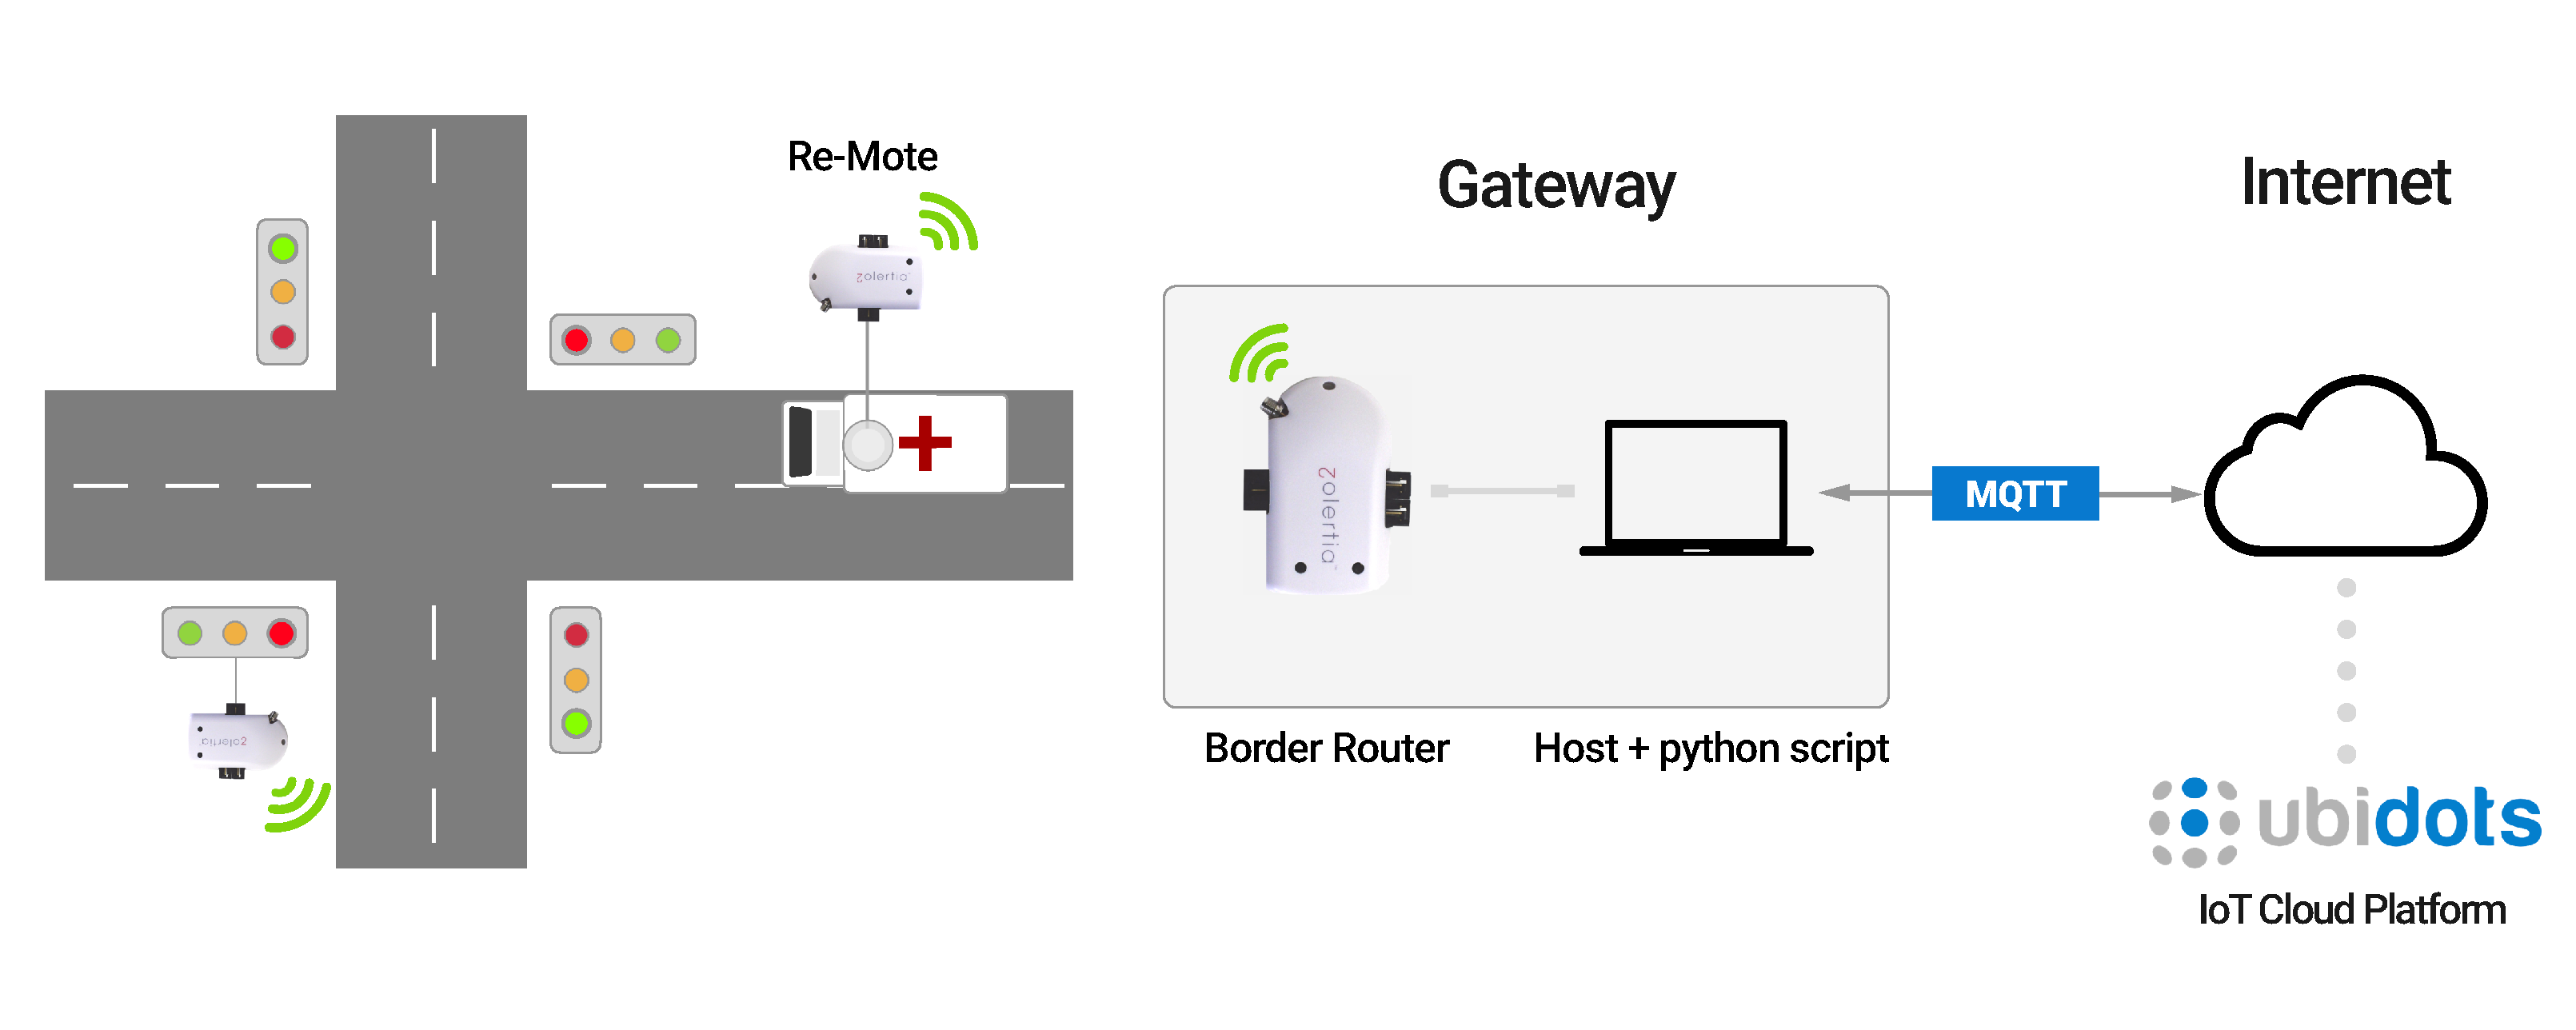
\includegraphics[width=4.5in]{Figures/ScenarioPaper.eps}
\caption{Architecture of  Iot-UTLC}
\label{fig:ScenarioPaper.eps}
\end{figure*}

Fig.
\ref{fig:ScenarioPaper.eps} shows the architecture of our IoT-UTLC with three layers.
From left to right,
	we have the WSN layer with connected traffic lights’ actuators,
	sensors and IEEE 802.15.4 transceivers.
The second part is the gateway of the WSN ensured by the BR and the Middleware \emph{i.e.} Python script launched by host computer.
The last layer is the Ubidots IoT Cloud Platform.
It is an open source solution used to collect and analyze WSN data.

\subsection{6LoWPAN, Contiki OS, Re-Mote and Border Router} \label{Sec:Contiki}

% 6LoWPAN
Our WSN is an IPv6 LowPower Wireless Personal Area Network (6LoWPAN) based on IEEE 802.15.4 stack.
It is well adapted to embedded wireless devices with energy aware constraint and for its capabilities to define a mesh topology.
Contiki Os\footnote{http://www.contiki-os.org/} has been used to implement networks' functions such as send,
	receive and data processing.
It is an embedded operating system with large open source community.
It supports Zolertia's Re-Motes \footnote{https://github.com/Zolertia/Resources/wiki/RE-Mote} and implements recent IEEE 802.15.4 standard specifications.
It also includes protocols such as RPL,
	CoAP and MQTT.
Furthermore,
	developer community is active and makes available source codes examples in order to help developing quickly new applications.

% Re-motes
Re-motes are compatible with our WSN specifications and our design model.
They are wireless devices with ultra-low power operation mode.
This choice has been motivated by long radio range of its IEEE 802.15.4 CC1200 transceiver,
	which transmits in the frequency band of 868-915 MHz.
In addition,
	each Re-Mote has analog and digital ports with a possibility to connect several analog sensors and actuators.
A Re-mote can be driven by a computer and become a sink and/or BR as well as a gateway between the 6LoWPAN network and the computer.

%\Figure{!htb}{1}{ethernetRouter.png}{Our Ethernet router}
\begin{figure}[!htb]
\centering
\includegraphics[width=2.5in]{Figures/ethernetRouter.png}
\caption{BR and sink combined on one board}
\label{fig:ethernetRouter.png}
\end{figure}

%[Explanation of how it works with the 2 radios,
To implement the previous model described in Section \ref{sec:Use Case and Model Design},
	we used six Re-motes:
	one for the BR,
	four to control the traffic lights and one Re-Mote to detect the arrival of a high priority vehicle near a crossing point.
For simplicity,
	we choose a touch sensor as a detecting device of priority vehicle.
We have developed four types of programs running on a Re-mote:
	traffic lights signs,
	sensors,
	high priority vehicle detecting device and BR function.
Sensors send periodically information to the IoT Cloud Platform with temperature,
	pressure or any relevant information that can be sensed.
As mentioned in the previous section,
	traffic lights are sub-divided into two modes:
	slaves and masters.
Masters nodes are the only ones to request the Middleware to change its light’s state and slaves simply change its state depending on received packets.
These roles are defined to reduce the overhead of network,
	redundancy and collisions,
	for instance.
Masters send periodically packets to request a change of state to the Middleware which forwards them to a Cloud platform.
 
BR node behaves differently compared to the other Re-motes.
The entries of its routing table are the list of Re-motes that pass through it.
It reroutes every packet it receives from its neighboring to host computer (or sink),
	which  creates a connection to the IoT Cloud platform.
Two options are possible to create our BR:
	i) separate the BR and sink and ii) combine both on the same device.
In our development,
	we worked on how to implement the sink and the BR nodes on the same Re-Mote board.
Fig.
\ref{fig:ethernetRouter.png} shows a prototype of the combined BR and sink,
	both connected to an ethernet interface.
Indeed,
	if the border router becomes an Ethernet router,
	there will no longer be any connection between the host/sink machine and the IoT Cloud platform.
Every Re-mote is able to connect independently to the IoT Cloud platform.
This approach has some advantages,
	such as the autonomy of the devices,
	but it generates an overhead requiring extra synchronization packets' exchange.
Therefore,
	we separate the sink and BR,
	since this solution is more flexible and resilient for our Testbed.

%The border router is at first a Re-mote,
%	but it has very different behavior and function.
%Indeed it has the task of re-routing every packet it receives from its cohorts to the serial port of the host machine.


%This machine will create a connection to the IoT Cloud platform and send the Re-motes messages to it and get responses for the Re-motes.
%The border router is a central node because it knows all to Re-motes in the 6LoWPAN which packets have transited by it.
%It acts as a Router and has a routing table of those Re-motes that pass through it.
%A web server page can be accessed to retrieve that information.
%We also tried a different approach of it.

 % [
%Transition with next paragraph => the use of MQTT to access the other "side" of the system
%Explanation of how it works (encapsulating the headers ...)
%]
%[
%Big part of how it works,
%what is good about it %New paragraph about the autonomous BR we were trying to develop
%Comparison between the 2 solutions
%]

% Autonomous BR
%As we have seen before,
%	this approach requires a Border Router linked the computer itself to the internet,
%	we tried to see if we can remove one part.
%Thus,
%	we added a component to the Re-mote in order to connect it directly to the internet via an Ethernet cable.

%[Transition with next paragraph => the use of MQTT to access the other "side" of the system]

\subsection{MQTT and UBIDOTS} \label{Sec:MQTT}

Fig.
\ref{fig:StackIoT.pdf} presents the layers of our UTLC network.
From bottom to up,
	the WSN network sense and/or detect,
	process and actuates traffic lights.
The second layer manages the 6 LowPan addressing and routing of packets throughout an IEEE 802.15.4 network.
The Edge Computing is the Middleware between the WSN and the Cloud platform.
For the setup of our UTLC,
	we start by establishing the access network of WSN.
The next step is to connect this network to Core network.
MQTT protocol controls three levels of QoS of exchanged packets from the WSN to the chosen Ubidots \footnote{https://ubidots.com/} Cloud platform.
It adopts IntServ approach for supporting quality of service in the network,
	it tags incoming packets in the border routers with different levels of priority.
Core routers read incoming packets headers and queue them according to their priority,
	packets with a high priority are sent faster compared to low priority ones.

MQTT ensures the QoS and publish/subscribe mechanisms through a broker.
The broker behaves as a server by filtering messages and organizing them in topics,
	which are strings used to filter messages and define the hierarchy of our data structure.
They allow us to organize how to receive multiple data from sensors such as temperature,
	up time,
	battery status and how to display them and obtain a real-time glance of our system.
It gets its messages from publishers and sends any modifications to entities,
	which that subscribed to the updated topics.
We used this mechanism with the Middleware in order to publish messages to the broker and get from the main topic the new values of the subscriber.

%We have seen in previous section what we used for our local sensors network, let's see now how we communicate with the IoT Cloud Platform. We will use MQTT which is a light-weight transportation protocol. In our solution, a python script will run an MQTT client to connect our WSN to Ubidots.

%MQTT ensures the QoS and publishes/subscribes mechanisms with a noteworthy topic organization. 

%The topics are strings used to filter messages and define the hierarchy of our data structure. They allow us to organize how to receive multiple data from sensors such as temperature, up time, battery status and how to display them and obtain a real-time glance of our system. 

%In addition, the broker behaves as a server by filtering messages and organize them in topics. It gets its messages from publishers and will send any modifications to entities which would have subscribed to the updated topics. We used this mechanism with the middleware in order to publish messages to the broker and get from the main topic the new values using the subscriber functionality.


The QoS feature of MQTT protocol manages network resources by handling retransmissions and guarantees the delivery of messages. It allows more control on messages by defining the level of guarantee. By default, the QoS is defined by three levels. The first one, level 0, is `At most one`. Level 1 is `At least one` where there is an acknowledgment to let the sender know that its packet has been received. Finally, level 2 `Exactly once` is the highest verification level with a request/response flows to ensure that only one message will be delivered and processed by the receiver. In our case, we applied levels 1 and 2 using \textit{paho.mqtt.client} Python library.  
%
%For example, subscribed clients could define the data QoS level of requested data by the source code shown bellow. 
For example, publisher of high priority data such as touch sensor has to indicate the highest level of QoS by the code shown bellow. 
We shared our implementation and its source codes at https://github.com/IoT-UTLC/contiki.
%
%\begin{footnotesize}
%\begin{lstlisting}
%# client receives a CONNACK response 
%# from the server.
%def on_connect(client, userdata, flags, rc):
%  print("Subscribed to " + MQTT_URL_TOPIC)
%  client.subscribe(MQTT_URL_TOPIC, 2) 
%  # 2nd arg is the QoS level to use 
%  # at maximum when it's needed
%\end{lstlisting}
%\end{footnotesize}

\begin{footnotesize}
\begin{lstlisting}
payload = json.dumps({"RoadA": data, "RoadB": 0})
res, mid = conn.publish(MQTT_URL_PUB, payload,
	  qos=int(QoS)) # QoS is QoS level to use 
\end{lstlisting}
\end{footnotesize}


%# The callback for when the client receives a CONNACK response from the server.
%def on_connect(client, userdata, flags, rc):
%	print("Connected with result code "+str(rc))
%	print("Subscribed to " + MQTT_URL_TOPIC)
%	client.subscribe(MQTT_URL_TOPIC, 2) 
                                                                                                                                                        
We experienced significant latency of high priority messages when we tested of IoT-UTLC mockup. Therefore, assessments of the MQTT protocol in our case provided significant information about its efficiency. 

%  For the end point the IoT Cloud platform,
% we wanted to be simple  %QoS and MQTT resilient by default (good implementation)
% Get relevant information from dashboard
% Access from anywhere (remote control possible)
% Structure our system / hierarchy
%
%As for the MQTT broker, we wanted an easy and powerful IoT Cloud Platform.
%It will be compatible with all technologies we chose for our prototyping,
%	so with an integration of MQTT and QoS levels.
%an IoT Cloud platform is a central point of the system as it keeps all the information about our WSN.
%Using the Cloud allows the system being accessible from anywhere on the internet.
%It is also a tool to filter and display relevant information in real-time from our system in the centralized dashboard.
%It can be possible to trigger some actions on the system via the dashboard.
%
%% Architecture
%Building this virtual infrastructure for this project has been challenging.
%we used MQTT topics mechanism to get the most of Ubidots to structure every data sent.
%We have a main topic which contains the states of the traffic light (RoadA and RoadB) in real time,
%	we created individual topics for every Re-mote acting as traffic lights or sensors.
%With this architecture,
%	we can have deep information on every device (such as its battery,
%	sensors data,
%	etc...).
%Moreover,
%	it could be scaled to match future needs.


%\Figure{!htb}{1}{cdf_distribution.pdf}{Normal,Gamma and Logistic distribution}
\begin{figure}[!htb]
\centering
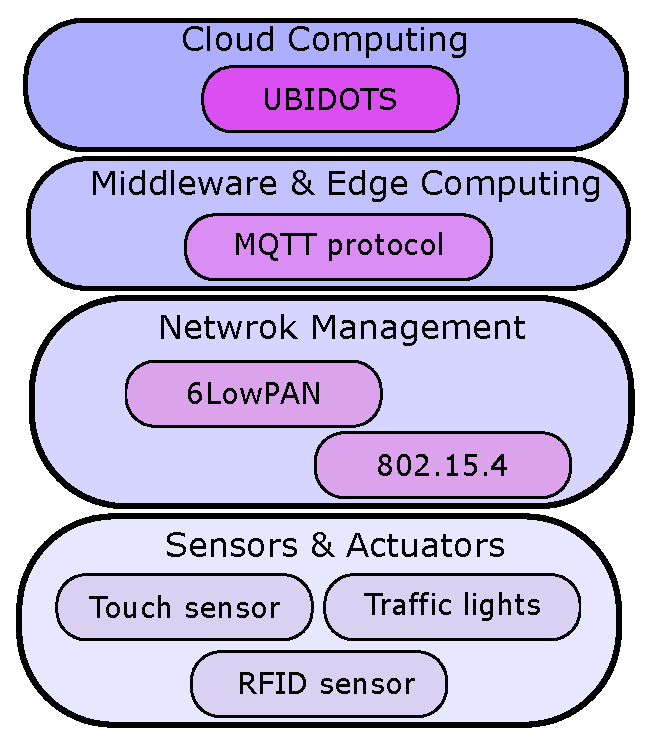
\includegraphics[width=2in]{Figures/StackIoTv1.eps}
\caption{UTLC network layers}
\label{fig:StackIoT.pdf}
\end{figure}

	\section{Results exploitation} \label{sec:Results exploitation}

% Initiation
%Below we report the results of applying the contagion process model to the Enron Email dataset.


% Final findings
%In summary,
%	results presented in this section show that if the trust coefficient between users is up to 0.8,
%	the vulnerability diffusion process through trust relationship is at its high level of speed.
%This what happens when a new information appears in a communication network and users forward it largely in the network.
%In addition,
%	this work gives a new insight to understand the relationship between trust,
%	reputation,
%	individual vulnerability and social vulnerability in the context of messaging services such as emails.


\subsection{Range}

\subsection{Response time}

\subsection{Connection speed}

\subsection{Power consumption}

	\section{Discussion} \label{sec:Conclusion}

%purpose
The purpose of the project was to find and examine a communication protocol that could be suitable for IoT applications,
	by investigating the current hardware,
	OS,
	and communication protocols and building a prototype from the selected choices.
What can be said about the investigation is that it is difficult to examine all candidates in detail;
	this means that a rough selection has to be made based on initial knowledge potentially discarding good options.
The general feeling is,
	however,
	that all of the examined candidates in this project were relevant and added valuable insights to the current technology status.
The assessment gave relevant and interesting results that improved the understanding in what IoT can be used for,
	and what further areas of investigation could be.
One of the most interesting areas of further investigation would be the RDC driver,
	as it directly affects the response time and thus also the connection speed.
Even though the power consumption was not in line with the expectations,
	the reason has been found and can be resolved.
Another conclusion is that IoT is not ready for real-time applications as the latency is much higher than expected,
	for the technologies assessed in this thesis,
	and also has a high spread.
As the latency increases for each subsequent network hop and the minimum observed latency per hop is 11ms,
	when using the always-on RDC,
	this type of communication will probably only be used for applications where response time can vary greatly,
	without affecting the functionality.
CoAP as a communication protocol shows a lot of promise when combined with 6LoWPAN and IEEE 802.15.4.
It performs well given its simplicity but has one disadvantage:
	the large overhead which comes from the MAC addressing fields in the IEEE 802.15.4 frame.
If this overhead could be reduced from the current 71\% to only 30%,
	the goodput would double.
A solution would be to use a similar mechanism as BLE where the packet size varies depending on application.
Each node also has computing time left as the MCU is more powerful  than needed for the given application;
	an improvement would be to use a less powerful MCU,
	like the ARM Cortex-M0+,
	to reduce the clock speed as suggested in the discussion.
When looking at the future-proof aspect the later suggestion is probably the better,
	as the clock then could be increased if more computing power is needed.
In the future,
	batteries will hopefully be able to store more energy,
	thus increasing the time between battery changes or reducing the battery size.


\chapter[4:''Qu'importe d'où viennent les questions, l'essentiel est d'où partent les réponses.'' - Slimane Benaïssa]{x-Sentilo}
	\begin{abstract}

% Problem
Most traffic light's control systems in smart cities are wired and have a semi-static behavior.
They are time-based, with pre-configured pattern and expensive cameras.
% Existing solutions
Although traffic lights can communicate wirelessly with incoming vehicles,
	they are less adapted to an urban environment.
If we consider light signs as an Internet of Things (IoT) network,
	one issue is to model thoroughly the change of signs' states and the Quality of Service (QoS) of this network.
In this paper,
	we propose a new architecture of Urban Traffic Light Control based on an IoT network (IoT-UTLC).
The objective is to interconnect both roads' infrastructures and traffic lights through an IoT platform.
We designed our IoT-UTLC by selecting motes and protocols of wireless sensor network (WSN).
Message Queuing Telemetry Transport (MQTT) protocol has been integrated to manage QoS.
It enables lights to adapt remotely to any situation and smoothly interrupt traffic light's classic cycles.
Our experimental results show that the MQTT protocol is efficient when the packets rate exceeds 35\% of traffic flow,
	it reduces traffic delay up to 0.05s at 90\% of congestion.
After verification and validation of our solution using a UPPAAL model checker,
	our system has been prototyped.
Motes' functions have been implemented on Contiki OS and connected through a 6LoWPAN/IEEE 802.15.4 network.
Time-stamping messages have been performed throughout the system to evaluate the MQTT protocol with different QoS levels.
In our experiments,
	we measured the Round-trip delay time (RTT) of messages exchanged between the WSN and IoT Cloud.
The results show that MQTT decreases the RTT when the Cumulative Distributed Function (CDF) of generated messages exceeds 35\%.

\end{abstract}
	\section{Introduction} \label{sec:Introduction}




\subsection{Problem Statement}

\subsection{Background}

\subsection{Purpose (Goal)}

\subsection{Limitations}

\subsection{Method}


% The structure 
This paper is organized as follows.
Section \ref{sec:Related work} elucidates summary of related works.
% Section \ref{sec:Background} provide the required background.
In section \ref{sec:Approach}, we propose our ... to ....
Section \ref{sec:Experimentation} evaluates the performance of our ... in terms of packet delivery ratio,
	throughput,
	and power consumption.
% Our findings are presented in section \ref{sec:Results}.
Section \ref{sec:Conclusion} concludes the article and gives some ideas for future work.


% Needs by statistics: Context Current needs


% Problematic Current bad state of the research


%Challenges
The difficulty to build such system is 


%Contribution 
In this work we 

% The structure 
The article is organized as follows.
Section \ref{sec:Related work} elucidates summary of related works,
In section \ref{sec:Approach}, we propose our ... to ....
Section \ref{sec:Experimentation} evaluate the performance of our ... in terms of packet delivery ratio,
	throughput,
	and power consumption.
Section \ref{sec:Conclusions} concludes the article and gives some ideas for future work.





	\section{Related work} \label{Sec:Related_Works}

Petri nets (PNs) are widely used for traffic light modelling and control \cite{huang_modular_2014}.
In  \cite{difebbraro_trafficresponsive_2006},
	deterministic-timed Petri Nets have been used to describe signalized intersections.
Undesirable deadlock states might appear when the nets are tested for some use cases.
The authors in \cite{febbraro_using_2009} have modified PNs models including  stochastic-time for one single signalized intersection.
Dotoli and Fanti \cite{dotoli_urban_2004} have built a colored timed PN with a deterministic modular framework,
	in which parts of the system,
	and even parts of the subsystems,
	can be specified and analyzed separately.
Examples using modularity are given in Soares and Vrancken \cite{dossantossoares_modular_2012},
	in which a p-timed PN is used for the control of a traffic signal in both main road and side streets.
However,
	formal characteristics of PNs (\emph{e.g.},
	deadlock and liveliness) haven’t been discussed.
Moreover,
	PNs suffer from a lack of analysis and verification tools.
To overcome these limits of PNs,
	we propose UPPAAL timed automata for design and verification of coherent state of cross road's traffic light.
UPPAAL is a timed-based modelling software with a graphical user interface.
It is the result of the research works of two universities UPPsala University in Sweden (UPP) and AALborg University in Denmark (AAL) \cite{david_uppaal_2015}.

In \cite{Web0},
	thermal cameras and on-street wired sensors detect vehicles and pedestrians in order to adapt the cycle of traffic light control systems.
However,
	such a solution can be expensive.
In addition,
	the system uses only its local view of the environment to detect the arrival of a vehicle.
Other solutions use recent technologies such as wireless sensors devices to limit the cost of thermal cameras and reduce the time needed to deploy sensors.
In \cite{tlig_decentralized_2014} and \cite{rose_internet_2015},
	the authors propose an adaptive system based on local wireless communication between lights and vehicles.
But such a solution requires a global interconnection between all road's users and infrastructure.
This problem comes from the rigid definition of technologies' standards.
Our work is not only limited to establish WSN,
	but it is scalable to interconnect heterogeneous wireless technologies through the Internet.
The obtained WSN intends to meet multiple QoS requirements of IoT applying the MQTT protocol.
In \cite{Silva2018},
	the latency of MQTT has been evaluated by calculating the average round-trip delay between two clients located in two different continents.
However,
	the evaluation has been limited to the impact of messages' size.
In our work,
	we consider the period of generated messages,
	and we calculate the RTT delays from WSN to Cloud IoT plateform.

In \cite{huang_modular_2014} \cite{difebbraro_trafficresponsive_2006} \cite{febbraro_using_2009} \cite{dossantossoares_modular_2012},
	the authors focus only on the structural analysis of their models and the transitions between colors of traffic lights.
However,
	the implementation of their models as a service in the Internet of smart cities has not been discussed.
Moreover,
	their methodology is not tested with any real traffic lights' Testbed.

	\section{Background} \label{sec:Background}

% \subsubsection{Hardware}

% \subsubsection{Operating system}

% \subsubsection{Communication protocol}


	\section{Proposed Framework} \label{sec:Approach}


% A generic scheme to solve the configuration selection problem and any other similar selection problem is given in this section..
% The genetic selection scheme consists of three main steps,
% 	the first step contains a set of small parallel fuzzy logic (FL)-based subsystems,
% 	the second step is a multiple criteria decision making (MCDM) system,
% 	and the third step is a genetic algorithm (GA)-based component to assign a suitable weight for the criteria in the second component.
% The scheme decision phase can be described in more detail as follows.


% \begin{figure}
% \placetextbox{0.75}{0.8}{
% 		\tiny \mywhiteblackbox{
% 		\begin{tabular}{l} 
% 			Source program \\\hline
% 	        Ada\\
% 	        C/C++\\
% 	        Java\\ 
% 		    Perl\\
% 		    Python\\
% 		    ...
% 	    \end{tabular}
% 	}
% }
% \end{figure}


% \Figure{h}{.5}{drawing.svg}{kjkjkj rd}
	% \begin{tikzpicture}
	% 	\scriptsize
	% 	% \node[draw,align=left,dashed, text width = 0.2\linewidth] at (3,6) {Criteria c1 fuzzy based control};

	% 	\node[draw,align=left,dashed, text width = .5cm, text height = .5cm] at (3,6) {Multiple criteria decision making};
	% 	\node[draw,align=left,dashed, text width = 2cm, text height = 2cm] at (6,6) {Multiple criteria decision making};
	% 	\node[draw,align=left,dashed, text width = 2cm, text height = 2cm] at (6,3) {Genetic algorithm to determine weights of criteria (w1, ..., wn)};
	% 	\draw[->,black,thick,dashed] (0,0) -- (1,1);
	% \end{tikzpicture}

% \textbf{Definition:} stopping criteria, population size P, and mutation probability pm\\
% \textbf{Generate} randomly the initial configurations \\
% \textbf{repeat:}\\
% . . . \textbf{for} each configuration do\\
% . . . . . . Train a model \& compute configuration's fitness\\
% . . . \textbf{end}\\
% . . . \textbf{for} each reproduction 1 ... P/2 do\\
% . . . . . . \textbf{Select:} 2 configurations based on fitness\\
% . . . . . . \textbf{Crossover:} Produce 2 child configurations\\
% . . . . . . \textbf{Mutate:} child configurations with pm\\
% . . . \textbf{end}\\
% \textbf{until} stopping criterion are met\\

% \State\textbf{Definition:} stopping criteria, population size P, and mutation probability pm\\
% \State\textbf{Generate} randomly the initial configurations


\begin{algorithm}
	 \KwData{QoS constraints}
	 \KwResult{Ranked configuration list}



\SetKwFunction{FMain}{Main}
\SetKwProg{GA}{GA}{:}{end}
\GA{}{
	\Repeat{stopping criterion is met}{
		\For{each configuration}{
			Train \& compute configuration's fitness
		}
		\For{each reproduction 1 ... P/2}{
			\textbf{Select:} 2 configurations based on fitness\;
			\textbf{Crossover:} Produce 2 child configurations\;
			\textbf{Mutate:} child configurations with pm\;
		}
	}
}

% \SetKwFunction{FMain}{Main}
% \SetKwProg{FL}{FL}{:}{end}
% \FL{}{
%     \eIf{$error \geq e$}{
%         Do that as well
%     }{
%         Do otherwise
%     }
%     \While{$something \not= 0$ }{	
%         $var1 \leftarrow var2$  	
%     }

% }
% \eIf{understand}{
%   go to next section\;
%   current section becomes this one\;
% }{
%   go back to the beginning of current section\;
% }

\caption{LoRa Transmission Parameter Selection}
\end{algorithm}
\medskip

The scheme selection process can be described following these five steps:

\begin{enumerate}
	\item According to the Semtech SX1276 specification\cite{lorasemtech}, there is 6720 possible settings ($s_{1}$, ... ,$s_{6720}$) and the framework has to select the most optimal one or to rank them according to their relevance.
	\item The first step of the selection process depends on multiple criteria up to i ($c_{1}$, ... , $c_{i}$).
		Different type of criteria can be measured from different sources to cover the maximum point of views,
		as example,
		the network server requirements, the applications requirements and the devices conditions.
	\item The Fuzzy Logic (FL) based subsystem gives an initial score for each configuration that reflects its relevance.
		The different sets of scores ($d_{1}$, ... ,$d_{i}$) are sent to the \ac{MCDM} in the $5^{th}$ step.
	\item At the same time,
			the genetic algorithm (GA) \cite{alkhawlani_access_2008} assigns a suitable weight ($w_{1}$, ... ,$w_{i}$) for each initial selection decision according to the objective function that is required by the application.
			% according to the importance and sensitivities of ANS criteria to the different characteristics of a wireless heterogeneous environment.
	\item Using the initial scores coming from the $3^{rd}$ step and the weights that are assigned using the $4^{th}$ step,
			the multi criteria decision making{} \ac{MCDM} will select the most relevant settings and rank them according to their reward.
\end{enumerate}


\Figure{h}{1}{genetic}{The proposed scheme for LoRa transmission parameters selection based on \ac{GA}, \ac{FL} and \ac{MCDM}}

	\section{Prototyping} \label{sec:Experimentation}

% Intro
We have prototyped the wireless sensors and actuator's network of traffic lights and roads on a mockup \footnote{https://github.com/IoT-UTLC/Resources/wiki} of real intersection in Paris with a scale of 1:68.
Our specifications have been defined considering the low-cost and energy efficiency of the solution.
This Testbed is a proof of concept of not limited to our use case as it is scalable for other applications.
For example,
	additional sensors of fine particules could be implanted bringing correlation between traffic jam and pollution.

\begin{figure*}[!htb]
\centering
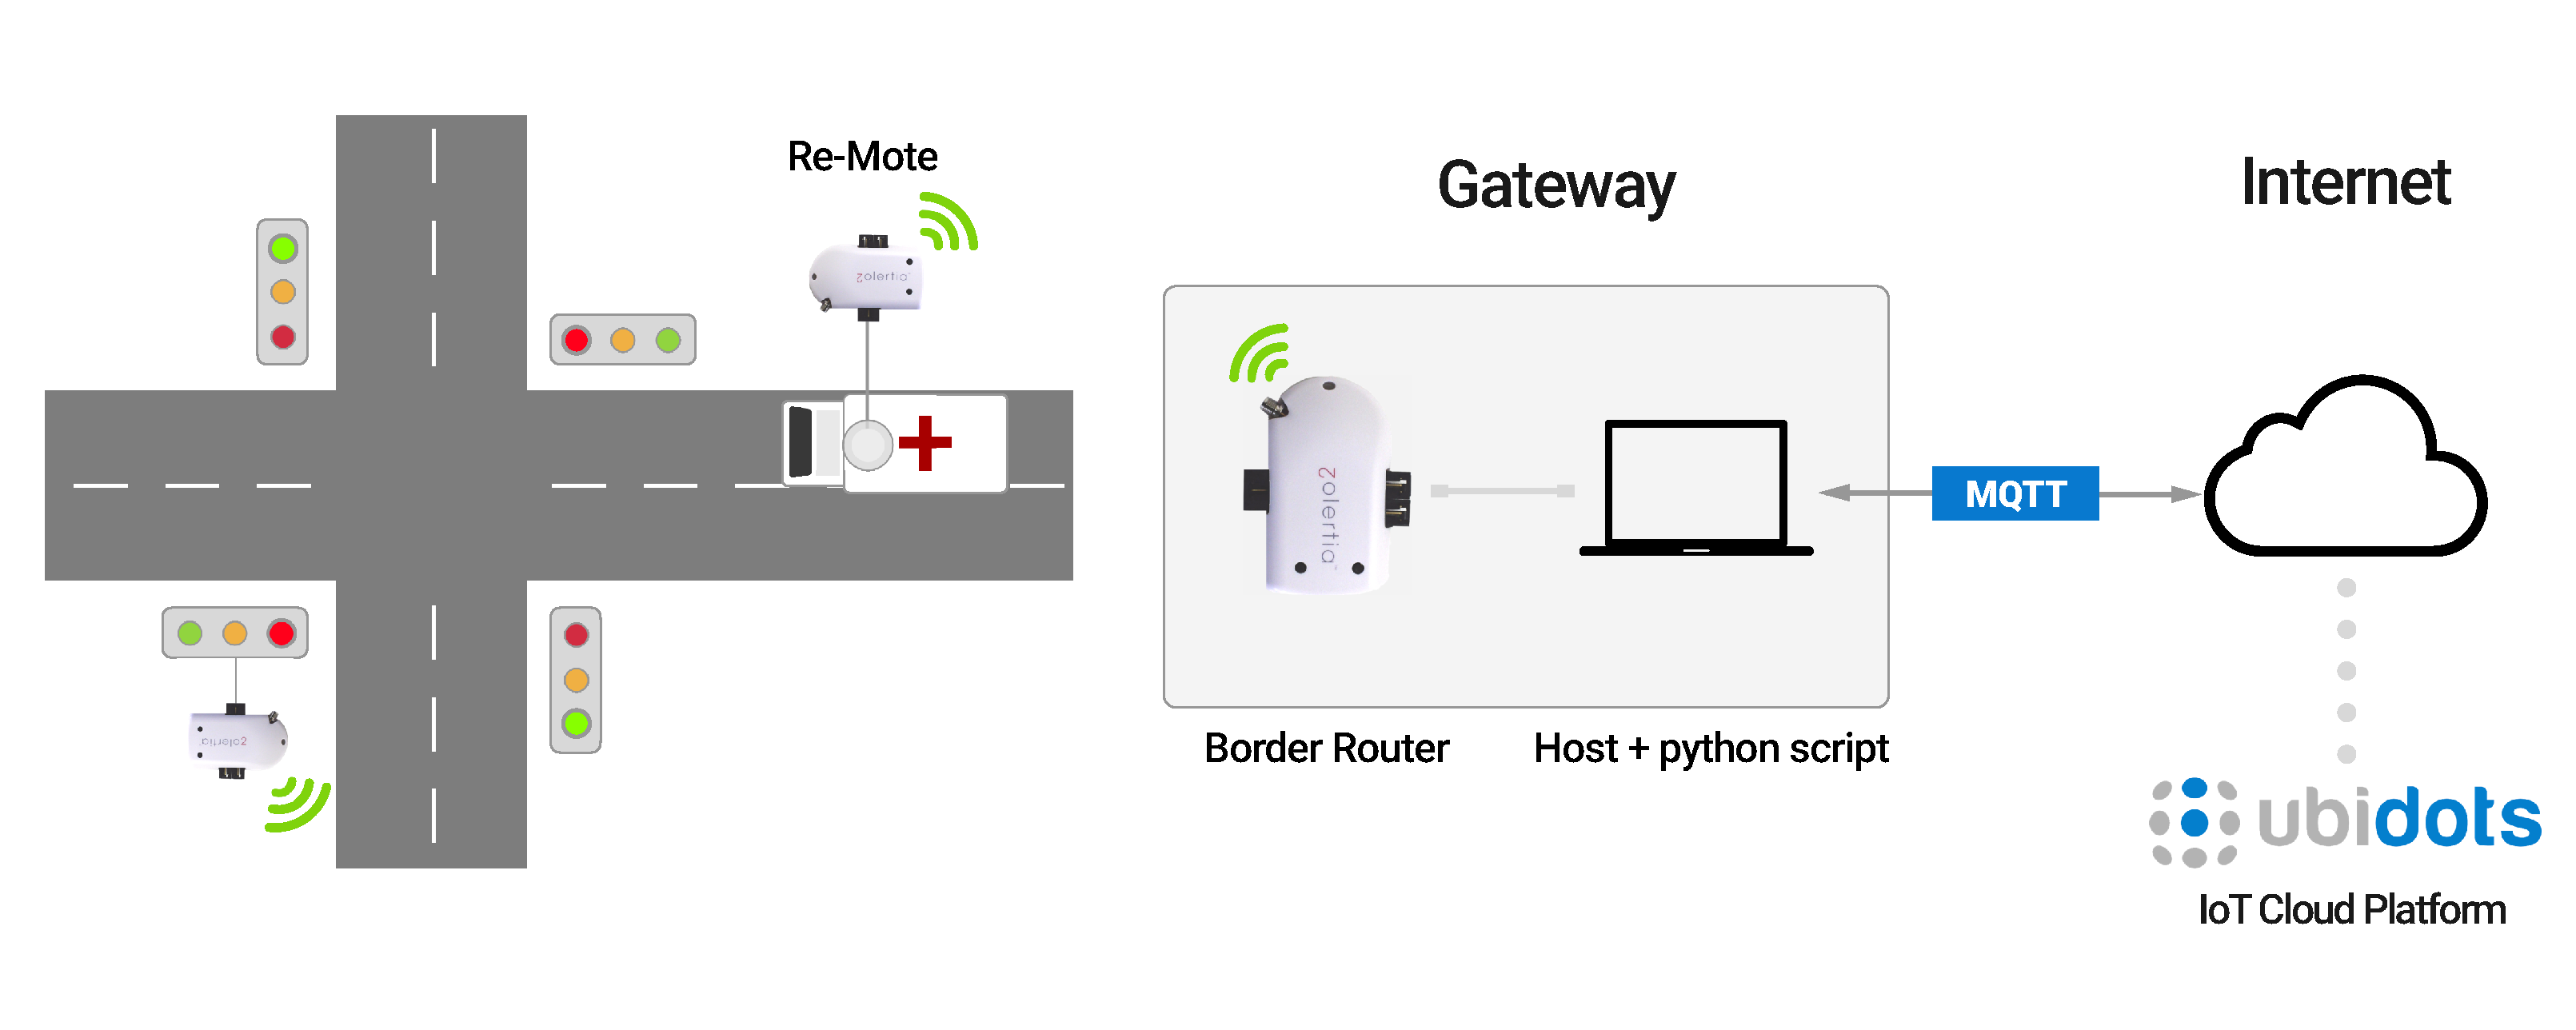
\includegraphics[width=4.5in]{Figures/ScenarioPaper.eps}
\caption{Architecture of  Iot-UTLC}
\label{fig:ScenarioPaper.eps}
\end{figure*}

Fig.
\ref{fig:ScenarioPaper.eps} shows the architecture of our IoT-UTLC with three layers.
From left to right,
	we have the WSN layer with connected traffic lights’ actuators,
	sensors and IEEE 802.15.4 transceivers.
The second part is the gateway of the WSN ensured by the BR and the Middleware \emph{i.e.} Python script launched by host computer.
The last layer is the Ubidots IoT Cloud Platform.
It is an open source solution used to collect and analyze WSN data.

\subsection{6LoWPAN, Contiki OS, Re-Mote and Border Router} \label{Sec:Contiki}

% 6LoWPAN
Our WSN is an IPv6 LowPower Wireless Personal Area Network (6LoWPAN) based on IEEE 802.15.4 stack.
It is well adapted to embedded wireless devices with energy aware constraint and for its capabilities to define a mesh topology.
Contiki Os\footnote{http://www.contiki-os.org/} has been used to implement networks' functions such as send,
	receive and data processing.
It is an embedded operating system with large open source community.
It supports Zolertia's Re-Motes \footnote{https://github.com/Zolertia/Resources/wiki/RE-Mote} and implements recent IEEE 802.15.4 standard specifications.
It also includes protocols such as RPL,
	CoAP and MQTT.
Furthermore,
	developer community is active and makes available source codes examples in order to help developing quickly new applications.

% Re-motes
Re-motes are compatible with our WSN specifications and our design model.
They are wireless devices with ultra-low power operation mode.
This choice has been motivated by long radio range of its IEEE 802.15.4 CC1200 transceiver,
	which transmits in the frequency band of 868-915 MHz.
In addition,
	each Re-Mote has analog and digital ports with a possibility to connect several analog sensors and actuators.
A Re-mote can be driven by a computer and become a sink and/or BR as well as a gateway between the 6LoWPAN network and the computer.

%\Figure{!htb}{1}{ethernetRouter.png}{Our Ethernet router}
\begin{figure}[!htb]
\centering
\includegraphics[width=2.5in]{Figures/ethernetRouter.png}
\caption{BR and sink combined on one board}
\label{fig:ethernetRouter.png}
\end{figure}

%[Explanation of how it works with the 2 radios,
To implement the previous model described in Section \ref{sec:Use Case and Model Design},
	we used six Re-motes:
	one for the BR,
	four to control the traffic lights and one Re-Mote to detect the arrival of a high priority vehicle near a crossing point.
For simplicity,
	we choose a touch sensor as a detecting device of priority vehicle.
We have developed four types of programs running on a Re-mote:
	traffic lights signs,
	sensors,
	high priority vehicle detecting device and BR function.
Sensors send periodically information to the IoT Cloud Platform with temperature,
	pressure or any relevant information that can be sensed.
As mentioned in the previous section,
	traffic lights are sub-divided into two modes:
	slaves and masters.
Masters nodes are the only ones to request the Middleware to change its light’s state and slaves simply change its state depending on received packets.
These roles are defined to reduce the overhead of network,
	redundancy and collisions,
	for instance.
Masters send periodically packets to request a change of state to the Middleware which forwards them to a Cloud platform.
 
BR node behaves differently compared to the other Re-motes.
The entries of its routing table are the list of Re-motes that pass through it.
It reroutes every packet it receives from its neighboring to host computer (or sink),
	which  creates a connection to the IoT Cloud platform.
Two options are possible to create our BR:
	i) separate the BR and sink and ii) combine both on the same device.
In our development,
	we worked on how to implement the sink and the BR nodes on the same Re-Mote board.
Fig.
\ref{fig:ethernetRouter.png} shows a prototype of the combined BR and sink,
	both connected to an ethernet interface.
Indeed,
	if the border router becomes an Ethernet router,
	there will no longer be any connection between the host/sink machine and the IoT Cloud platform.
Every Re-mote is able to connect independently to the IoT Cloud platform.
This approach has some advantages,
	such as the autonomy of the devices,
	but it generates an overhead requiring extra synchronization packets' exchange.
Therefore,
	we separate the sink and BR,
	since this solution is more flexible and resilient for our Testbed.

%The border router is at first a Re-mote,
%	but it has very different behavior and function.
%Indeed it has the task of re-routing every packet it receives from its cohorts to the serial port of the host machine.


%This machine will create a connection to the IoT Cloud platform and send the Re-motes messages to it and get responses for the Re-motes.
%The border router is a central node because it knows all to Re-motes in the 6LoWPAN which packets have transited by it.
%It acts as a Router and has a routing table of those Re-motes that pass through it.
%A web server page can be accessed to retrieve that information.
%We also tried a different approach of it.

 % [
%Transition with next paragraph => the use of MQTT to access the other "side" of the system
%Explanation of how it works (encapsulating the headers ...)
%]
%[
%Big part of how it works,
%what is good about it %New paragraph about the autonomous BR we were trying to develop
%Comparison between the 2 solutions
%]

% Autonomous BR
%As we have seen before,
%	this approach requires a Border Router linked the computer itself to the internet,
%	we tried to see if we can remove one part.
%Thus,
%	we added a component to the Re-mote in order to connect it directly to the internet via an Ethernet cable.

%[Transition with next paragraph => the use of MQTT to access the other "side" of the system]

\subsection{MQTT and UBIDOTS} \label{Sec:MQTT}

Fig.
\ref{fig:StackIoT.pdf} presents the layers of our UTLC network.
From bottom to up,
	the WSN network sense and/or detect,
	process and actuates traffic lights.
The second layer manages the 6 LowPan addressing and routing of packets throughout an IEEE 802.15.4 network.
The Edge Computing is the Middleware between the WSN and the Cloud platform.
For the setup of our UTLC,
	we start by establishing the access network of WSN.
The next step is to connect this network to Core network.
MQTT protocol controls three levels of QoS of exchanged packets from the WSN to the chosen Ubidots \footnote{https://ubidots.com/} Cloud platform.
It adopts IntServ approach for supporting quality of service in the network,
	it tags incoming packets in the border routers with different levels of priority.
Core routers read incoming packets headers and queue them according to their priority,
	packets with a high priority are sent faster compared to low priority ones.

MQTT ensures the QoS and publish/subscribe mechanisms through a broker.
The broker behaves as a server by filtering messages and organizing them in topics,
	which are strings used to filter messages and define the hierarchy of our data structure.
They allow us to organize how to receive multiple data from sensors such as temperature,
	up time,
	battery status and how to display them and obtain a real-time glance of our system.
It gets its messages from publishers and sends any modifications to entities,
	which that subscribed to the updated topics.
We used this mechanism with the Middleware in order to publish messages to the broker and get from the main topic the new values of the subscriber.

%We have seen in previous section what we used for our local sensors network, let's see now how we communicate with the IoT Cloud Platform. We will use MQTT which is a light-weight transportation protocol. In our solution, a python script will run an MQTT client to connect our WSN to Ubidots.

%MQTT ensures the QoS and publishes/subscribes mechanisms with a noteworthy topic organization. 

%The topics are strings used to filter messages and define the hierarchy of our data structure. They allow us to organize how to receive multiple data from sensors such as temperature, up time, battery status and how to display them and obtain a real-time glance of our system. 

%In addition, the broker behaves as a server by filtering messages and organize them in topics. It gets its messages from publishers and will send any modifications to entities which would have subscribed to the updated topics. We used this mechanism with the middleware in order to publish messages to the broker and get from the main topic the new values using the subscriber functionality.


The QoS feature of MQTT protocol manages network resources by handling retransmissions and guarantees the delivery of messages. It allows more control on messages by defining the level of guarantee. By default, the QoS is defined by three levels. The first one, level 0, is `At most one`. Level 1 is `At least one` where there is an acknowledgment to let the sender know that its packet has been received. Finally, level 2 `Exactly once` is the highest verification level with a request/response flows to ensure that only one message will be delivered and processed by the receiver. In our case, we applied levels 1 and 2 using \textit{paho.mqtt.client} Python library.  
%
%For example, subscribed clients could define the data QoS level of requested data by the source code shown bellow. 
For example, publisher of high priority data such as touch sensor has to indicate the highest level of QoS by the code shown bellow. 
We shared our implementation and its source codes at https://github.com/IoT-UTLC/contiki.
%
%\begin{footnotesize}
%\begin{lstlisting}
%# client receives a CONNACK response 
%# from the server.
%def on_connect(client, userdata, flags, rc):
%  print("Subscribed to " + MQTT_URL_TOPIC)
%  client.subscribe(MQTT_URL_TOPIC, 2) 
%  # 2nd arg is the QoS level to use 
%  # at maximum when it's needed
%\end{lstlisting}
%\end{footnotesize}

\begin{footnotesize}
\begin{lstlisting}
payload = json.dumps({"RoadA": data, "RoadB": 0})
res, mid = conn.publish(MQTT_URL_PUB, payload,
	  qos=int(QoS)) # QoS is QoS level to use 
\end{lstlisting}
\end{footnotesize}


%# The callback for when the client receives a CONNACK response from the server.
%def on_connect(client, userdata, flags, rc):
%	print("Connected with result code "+str(rc))
%	print("Subscribed to " + MQTT_URL_TOPIC)
%	client.subscribe(MQTT_URL_TOPIC, 2) 
                                                                                                                                                        
We experienced significant latency of high priority messages when we tested of IoT-UTLC mockup. Therefore, assessments of the MQTT protocol in our case provided significant information about its efficiency. 

%  For the end point the IoT Cloud platform,
% we wanted to be simple  %QoS and MQTT resilient by default (good implementation)
% Get relevant information from dashboard
% Access from anywhere (remote control possible)
% Structure our system / hierarchy
%
%As for the MQTT broker, we wanted an easy and powerful IoT Cloud Platform.
%It will be compatible with all technologies we chose for our prototyping,
%	so with an integration of MQTT and QoS levels.
%an IoT Cloud platform is a central point of the system as it keeps all the information about our WSN.
%Using the Cloud allows the system being accessible from anywhere on the internet.
%It is also a tool to filter and display relevant information in real-time from our system in the centralized dashboard.
%It can be possible to trigger some actions on the system via the dashboard.
%
%% Architecture
%Building this virtual infrastructure for this project has been challenging.
%we used MQTT topics mechanism to get the most of Ubidots to structure every data sent.
%We have a main topic which contains the states of the traffic light (RoadA and RoadB) in real time,
%	we created individual topics for every Re-mote acting as traffic lights or sensors.
%With this architecture,
%	we can have deep information on every device (such as its battery,
%	sensors data,
%	etc...).
%Moreover,
%	it could be scaled to match future needs.


%\Figure{!htb}{1}{cdf_distribution.pdf}{Normal,Gamma and Logistic distribution}
\begin{figure}[!htb]
\centering
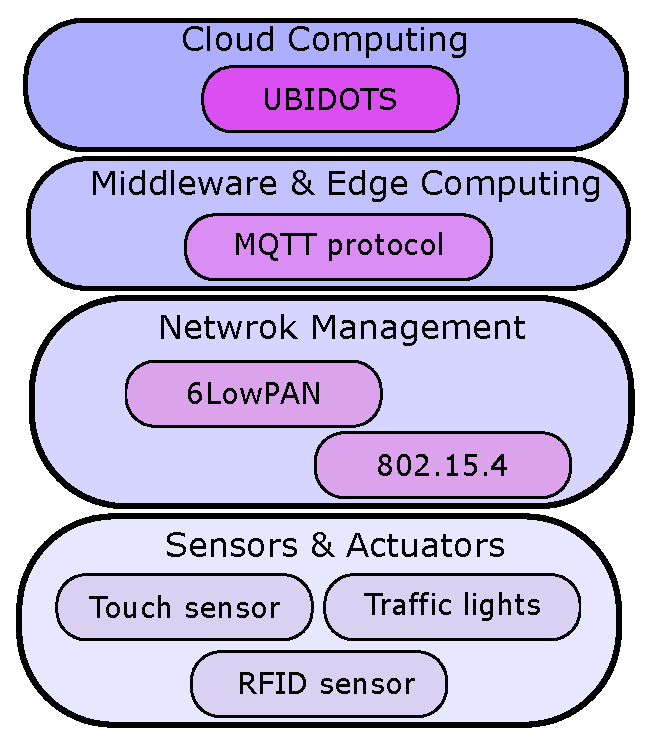
\includegraphics[width=2in]{Figures/StackIoTv1.eps}
\caption{UTLC network layers}
\label{fig:StackIoT.pdf}
\end{figure}

	\section{Results exploitation} \label{sec:Results exploitation}

% Initiation
%Below we report the results of applying the contagion process model to the Enron Email dataset.


% Final findings
%In summary,
%	results presented in this section show that if the trust coefficient between users is up to 0.8,
%	the vulnerability diffusion process through trust relationship is at its high level of speed.
%This what happens when a new information appears in a communication network and users forward it largely in the network.
%In addition,
%	this work gives a new insight to understand the relationship between trust,
%	reputation,
%	individual vulnerability and social vulnerability in the context of messaging services such as emails.


\subsection{Range}

\subsection{Response time}

\subsection{Connection speed}

\subsection{Power consumption}

	\section{Discussion} \label{sec:Conclusion}

%purpose
The purpose of the project was to find and examine a communication protocol that could be suitable for IoT applications,
	by investigating the current hardware,
	OS,
	and communication protocols and building a prototype from the selected choices.
What can be said about the investigation is that it is difficult to examine all candidates in detail;
	this means that a rough selection has to be made based on initial knowledge potentially discarding good options.
The general feeling is,
	however,
	that all of the examined candidates in this project were relevant and added valuable insights to the current technology status.
The assessment gave relevant and interesting results that improved the understanding in what IoT can be used for,
	and what further areas of investigation could be.
One of the most interesting areas of further investigation would be the RDC driver,
	as it directly affects the response time and thus also the connection speed.
Even though the power consumption was not in line with the expectations,
	the reason has been found and can be resolved.
Another conclusion is that IoT is not ready for real-time applications as the latency is much higher than expected,
	for the technologies assessed in this thesis,
	and also has a high spread.
As the latency increases for each subsequent network hop and the minimum observed latency per hop is 11ms,
	when using the always-on RDC,
	this type of communication will probably only be used for applications where response time can vary greatly,
	without affecting the functionality.
CoAP as a communication protocol shows a lot of promise when combined with 6LoWPAN and IEEE 802.15.4.
It performs well given its simplicity but has one disadvantage:
	the large overhead which comes from the MAC addressing fields in the IEEE 802.15.4 frame.
If this overhead could be reduced from the current 71\% to only 30%,
	the goodput would double.
A solution would be to use a similar mechanism as BLE where the packet size varies depending on application.
Each node also has computing time left as the MCU is more powerful  than needed for the given application;
	an improvement would be to use a less powerful MCU,
	like the ARM Cortex-M0+,
	to reduce the clock speed as suggested in the discussion.
When looking at the future-proof aspect the later suggestion is probably the better,
	as the clock then could be increased if more computing power is needed.
In the future,
	batteries will hopefully be able to store more energy,
	thus increasing the time between battery changes or reducing the battery size.


\chapter[5:''I can’t remember the last day I didn’t train'' - Michael Phelps]{x-Long paper}
	\begin{abstract}

% Problem
Most traffic light's control systems in smart cities are wired and have a semi-static behavior.
They are time-based, with pre-configured pattern and expensive cameras.
% Existing solutions
Although traffic lights can communicate wirelessly with incoming vehicles,
	they are less adapted to an urban environment.
If we consider light signs as an Internet of Things (IoT) network,
	one issue is to model thoroughly the change of signs' states and the Quality of Service (QoS) of this network.
In this paper,
	we propose a new architecture of Urban Traffic Light Control based on an IoT network (IoT-UTLC).
The objective is to interconnect both roads' infrastructures and traffic lights through an IoT platform.
We designed our IoT-UTLC by selecting motes and protocols of wireless sensor network (WSN).
Message Queuing Telemetry Transport (MQTT) protocol has been integrated to manage QoS.
It enables lights to adapt remotely to any situation and smoothly interrupt traffic light's classic cycles.
Our experimental results show that the MQTT protocol is efficient when the packets rate exceeds 35\% of traffic flow,
	it reduces traffic delay up to 0.05s at 90\% of congestion.
After verification and validation of our solution using a UPPAAL model checker,
	our system has been prototyped.
Motes' functions have been implemented on Contiki OS and connected through a 6LoWPAN/IEEE 802.15.4 network.
Time-stamping messages have been performed throughout the system to evaluate the MQTT protocol with different QoS levels.
In our experiments,
	we measured the Round-trip delay time (RTT) of messages exchanged between the WSN and IoT Cloud.
The results show that MQTT decreases the RTT when the Cumulative Distributed Function (CDF) of generated messages exceeds 35\%.

\end{abstract}
	\section{Introduction} \label{sec:Introduction}




\subsection{Problem Statement}

\subsection{Background}

\subsection{Purpose (Goal)}

\subsection{Limitations}

\subsection{Method}


% The structure 
This paper is organized as follows.
Section \ref{sec:Related work} elucidates summary of related works.
% Section \ref{sec:Background} provide the required background.
In section \ref{sec:Approach}, we propose our ... to ....
Section \ref{sec:Experimentation} evaluates the performance of our ... in terms of packet delivery ratio,
	throughput,
	and power consumption.
% Our findings are presented in section \ref{sec:Results}.
Section \ref{sec:Conclusion} concludes the article and gives some ideas for future work.


% Needs by statistics: Context Current needs


% Problematic Current bad state of the research


%Challenges
The difficulty to build such system is 


%Contribution 
In this work we 

% The structure 
The article is organized as follows.
Section \ref{sec:Related work} elucidates summary of related works,
In section \ref{sec:Approach}, we propose our ... to ....
Section \ref{sec:Experimentation} evaluate the performance of our ... in terms of packet delivery ratio,
	throughput,
	and power consumption.
Section \ref{sec:Conclusions} concludes the article and gives some ideas for future work.





	\section{Related work} \label{Sec:Related_Works}

Petri nets (PNs) are widely used for traffic light modelling and control \cite{huang_modular_2014}.
In  \cite{difebbraro_trafficresponsive_2006},
	deterministic-timed Petri Nets have been used to describe signalized intersections.
Undesirable deadlock states might appear when the nets are tested for some use cases.
The authors in \cite{febbraro_using_2009} have modified PNs models including  stochastic-time for one single signalized intersection.
Dotoli and Fanti \cite{dotoli_urban_2004} have built a colored timed PN with a deterministic modular framework,
	in which parts of the system,
	and even parts of the subsystems,
	can be specified and analyzed separately.
Examples using modularity are given in Soares and Vrancken \cite{dossantossoares_modular_2012},
	in which a p-timed PN is used for the control of a traffic signal in both main road and side streets.
However,
	formal characteristics of PNs (\emph{e.g.},
	deadlock and liveliness) haven’t been discussed.
Moreover,
	PNs suffer from a lack of analysis and verification tools.
To overcome these limits of PNs,
	we propose UPPAAL timed automata for design and verification of coherent state of cross road's traffic light.
UPPAAL is a timed-based modelling software with a graphical user interface.
It is the result of the research works of two universities UPPsala University in Sweden (UPP) and AALborg University in Denmark (AAL) \cite{david_uppaal_2015}.

In \cite{Web0},
	thermal cameras and on-street wired sensors detect vehicles and pedestrians in order to adapt the cycle of traffic light control systems.
However,
	such a solution can be expensive.
In addition,
	the system uses only its local view of the environment to detect the arrival of a vehicle.
Other solutions use recent technologies such as wireless sensors devices to limit the cost of thermal cameras and reduce the time needed to deploy sensors.
In \cite{tlig_decentralized_2014} and \cite{rose_internet_2015},
	the authors propose an adaptive system based on local wireless communication between lights and vehicles.
But such a solution requires a global interconnection between all road's users and infrastructure.
This problem comes from the rigid definition of technologies' standards.
Our work is not only limited to establish WSN,
	but it is scalable to interconnect heterogeneous wireless technologies through the Internet.
The obtained WSN intends to meet multiple QoS requirements of IoT applying the MQTT protocol.
In \cite{Silva2018},
	the latency of MQTT has been evaluated by calculating the average round-trip delay between two clients located in two different continents.
However,
	the evaluation has been limited to the impact of messages' size.
In our work,
	we consider the period of generated messages,
	and we calculate the RTT delays from WSN to Cloud IoT plateform.

In \cite{huang_modular_2014} \cite{difebbraro_trafficresponsive_2006} \cite{febbraro_using_2009} \cite{dossantossoares_modular_2012},
	the authors focus only on the structural analysis of their models and the transitions between colors of traffic lights.
However,
	the implementation of their models as a service in the Internet of smart cities has not been discussed.
Moreover,
	their methodology is not tested with any real traffic lights' Testbed.

	\section{Background} \label{sec:Background}

% \subsubsection{Hardware}

% \subsubsection{Operating system}

% \subsubsection{Communication protocol}


	\section{Proposed Framework} \label{sec:Approach}


% A generic scheme to solve the configuration selection problem and any other similar selection problem is given in this section..
% The genetic selection scheme consists of three main steps,
% 	the first step contains a set of small parallel fuzzy logic (FL)-based subsystems,
% 	the second step is a multiple criteria decision making (MCDM) system,
% 	and the third step is a genetic algorithm (GA)-based component to assign a suitable weight for the criteria in the second component.
% The scheme decision phase can be described in more detail as follows.


% \begin{figure}
% \placetextbox{0.75}{0.8}{
% 		\tiny \mywhiteblackbox{
% 		\begin{tabular}{l} 
% 			Source program \\\hline
% 	        Ada\\
% 	        C/C++\\
% 	        Java\\ 
% 		    Perl\\
% 		    Python\\
% 		    ...
% 	    \end{tabular}
% 	}
% }
% \end{figure}


% \Figure{h}{.5}{drawing.svg}{kjkjkj rd}
	% \begin{tikzpicture}
	% 	\scriptsize
	% 	% \node[draw,align=left,dashed, text width = 0.2\linewidth] at (3,6) {Criteria c1 fuzzy based control};

	% 	\node[draw,align=left,dashed, text width = .5cm, text height = .5cm] at (3,6) {Multiple criteria decision making};
	% 	\node[draw,align=left,dashed, text width = 2cm, text height = 2cm] at (6,6) {Multiple criteria decision making};
	% 	\node[draw,align=left,dashed, text width = 2cm, text height = 2cm] at (6,3) {Genetic algorithm to determine weights of criteria (w1, ..., wn)};
	% 	\draw[->,black,thick,dashed] (0,0) -- (1,1);
	% \end{tikzpicture}

% \textbf{Definition:} stopping criteria, population size P, and mutation probability pm\\
% \textbf{Generate} randomly the initial configurations \\
% \textbf{repeat:}\\
% . . . \textbf{for} each configuration do\\
% . . . . . . Train a model \& compute configuration's fitness\\
% . . . \textbf{end}\\
% . . . \textbf{for} each reproduction 1 ... P/2 do\\
% . . . . . . \textbf{Select:} 2 configurations based on fitness\\
% . . . . . . \textbf{Crossover:} Produce 2 child configurations\\
% . . . . . . \textbf{Mutate:} child configurations with pm\\
% . . . \textbf{end}\\
% \textbf{until} stopping criterion are met\\

% \State\textbf{Definition:} stopping criteria, population size P, and mutation probability pm\\
% \State\textbf{Generate} randomly the initial configurations


\begin{algorithm}
	 \KwData{QoS constraints}
	 \KwResult{Ranked configuration list}



\SetKwFunction{FMain}{Main}
\SetKwProg{GA}{GA}{:}{end}
\GA{}{
	\Repeat{stopping criterion is met}{
		\For{each configuration}{
			Train \& compute configuration's fitness
		}
		\For{each reproduction 1 ... P/2}{
			\textbf{Select:} 2 configurations based on fitness\;
			\textbf{Crossover:} Produce 2 child configurations\;
			\textbf{Mutate:} child configurations with pm\;
		}
	}
}

% \SetKwFunction{FMain}{Main}
% \SetKwProg{FL}{FL}{:}{end}
% \FL{}{
%     \eIf{$error \geq e$}{
%         Do that as well
%     }{
%         Do otherwise
%     }
%     \While{$something \not= 0$ }{	
%         $var1 \leftarrow var2$  	
%     }

% }
% \eIf{understand}{
%   go to next section\;
%   current section becomes this one\;
% }{
%   go back to the beginning of current section\;
% }

\caption{LoRa Transmission Parameter Selection}
\end{algorithm}
\medskip

The scheme selection process can be described following these five steps:

\begin{enumerate}
	\item According to the Semtech SX1276 specification\cite{lorasemtech}, there is 6720 possible settings ($s_{1}$, ... ,$s_{6720}$) and the framework has to select the most optimal one or to rank them according to their relevance.
	\item The first step of the selection process depends on multiple criteria up to i ($c_{1}$, ... , $c_{i}$).
		Different type of criteria can be measured from different sources to cover the maximum point of views,
		as example,
		the network server requirements, the applications requirements and the devices conditions.
	\item The Fuzzy Logic (FL) based subsystem gives an initial score for each configuration that reflects its relevance.
		The different sets of scores ($d_{1}$, ... ,$d_{i}$) are sent to the \ac{MCDM} in the $5^{th}$ step.
	\item At the same time,
			the genetic algorithm (GA) \cite{alkhawlani_access_2008} assigns a suitable weight ($w_{1}$, ... ,$w_{i}$) for each initial selection decision according to the objective function that is required by the application.
			% according to the importance and sensitivities of ANS criteria to the different characteristics of a wireless heterogeneous environment.
	\item Using the initial scores coming from the $3^{rd}$ step and the weights that are assigned using the $4^{th}$ step,
			the multi criteria decision making{} \ac{MCDM} will select the most relevant settings and rank them according to their reward.
\end{enumerate}


\Figure{h}{1}{genetic}{The proposed scheme for LoRa transmission parameters selection based on \ac{GA}, \ac{FL} and \ac{MCDM}}

	\section{Prototyping} \label{sec:Experimentation}

% Intro
We have prototyped the wireless sensors and actuator's network of traffic lights and roads on a mockup \footnote{https://github.com/IoT-UTLC/Resources/wiki} of real intersection in Paris with a scale of 1:68.
Our specifications have been defined considering the low-cost and energy efficiency of the solution.
This Testbed is a proof of concept of not limited to our use case as it is scalable for other applications.
For example,
	additional sensors of fine particules could be implanted bringing correlation between traffic jam and pollution.

\begin{figure*}[!htb]
\centering
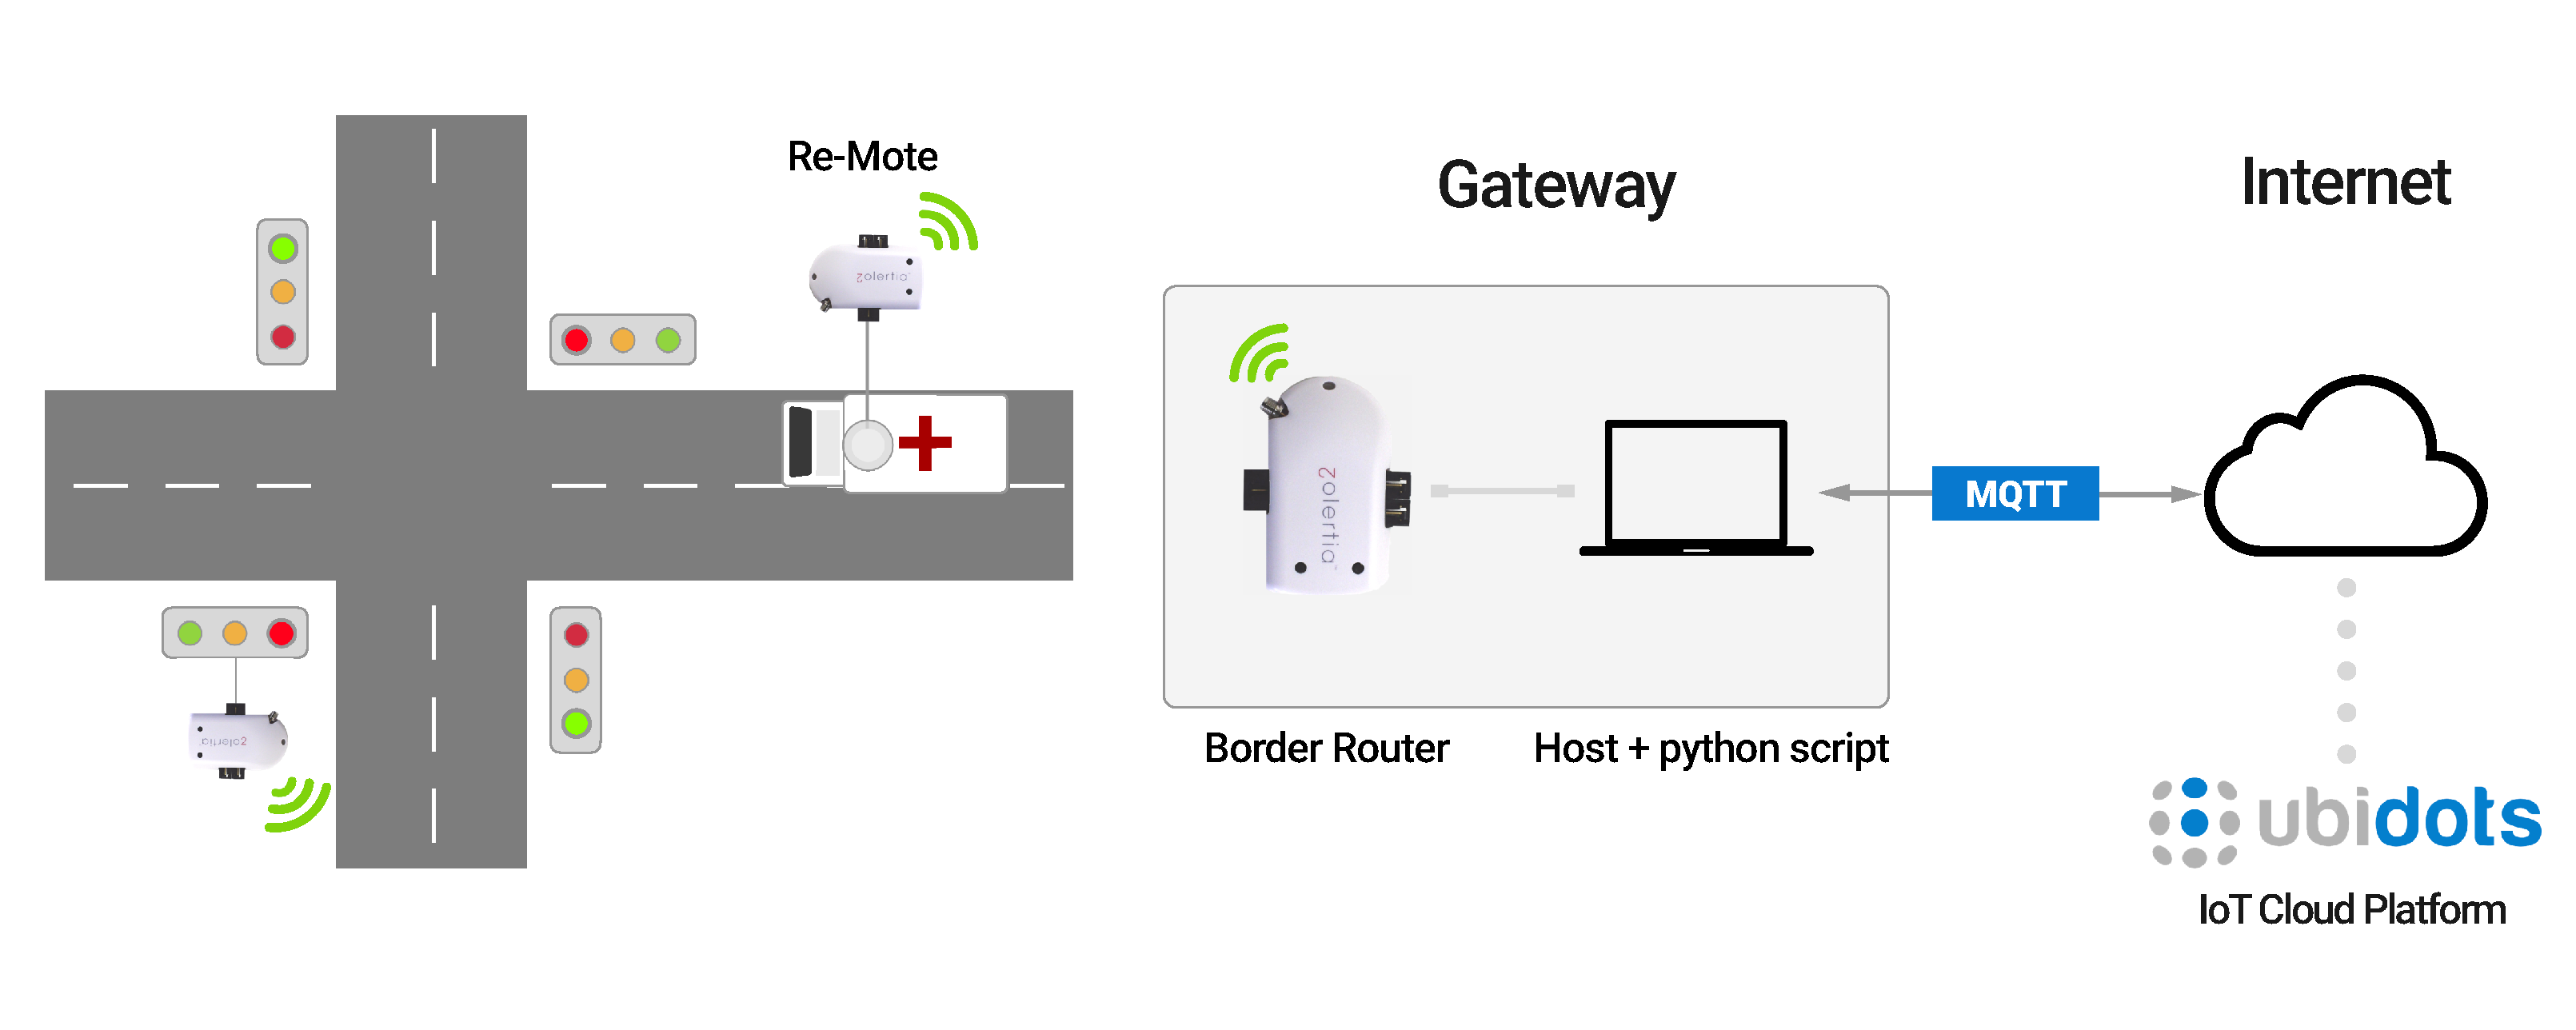
\includegraphics[width=4.5in]{Figures/ScenarioPaper.eps}
\caption{Architecture of  Iot-UTLC}
\label{fig:ScenarioPaper.eps}
\end{figure*}

Fig.
\ref{fig:ScenarioPaper.eps} shows the architecture of our IoT-UTLC with three layers.
From left to right,
	we have the WSN layer with connected traffic lights’ actuators,
	sensors and IEEE 802.15.4 transceivers.
The second part is the gateway of the WSN ensured by the BR and the Middleware \emph{i.e.} Python script launched by host computer.
The last layer is the Ubidots IoT Cloud Platform.
It is an open source solution used to collect and analyze WSN data.

\subsection{6LoWPAN, Contiki OS, Re-Mote and Border Router} \label{Sec:Contiki}

% 6LoWPAN
Our WSN is an IPv6 LowPower Wireless Personal Area Network (6LoWPAN) based on IEEE 802.15.4 stack.
It is well adapted to embedded wireless devices with energy aware constraint and for its capabilities to define a mesh topology.
Contiki Os\footnote{http://www.contiki-os.org/} has been used to implement networks' functions such as send,
	receive and data processing.
It is an embedded operating system with large open source community.
It supports Zolertia's Re-Motes \footnote{https://github.com/Zolertia/Resources/wiki/RE-Mote} and implements recent IEEE 802.15.4 standard specifications.
It also includes protocols such as RPL,
	CoAP and MQTT.
Furthermore,
	developer community is active and makes available source codes examples in order to help developing quickly new applications.

% Re-motes
Re-motes are compatible with our WSN specifications and our design model.
They are wireless devices with ultra-low power operation mode.
This choice has been motivated by long radio range of its IEEE 802.15.4 CC1200 transceiver,
	which transmits in the frequency band of 868-915 MHz.
In addition,
	each Re-Mote has analog and digital ports with a possibility to connect several analog sensors and actuators.
A Re-mote can be driven by a computer and become a sink and/or BR as well as a gateway between the 6LoWPAN network and the computer.

%\Figure{!htb}{1}{ethernetRouter.png}{Our Ethernet router}
\begin{figure}[!htb]
\centering
\includegraphics[width=2.5in]{Figures/ethernetRouter.png}
\caption{BR and sink combined on one board}
\label{fig:ethernetRouter.png}
\end{figure}

%[Explanation of how it works with the 2 radios,
To implement the previous model described in Section \ref{sec:Use Case and Model Design},
	we used six Re-motes:
	one for the BR,
	four to control the traffic lights and one Re-Mote to detect the arrival of a high priority vehicle near a crossing point.
For simplicity,
	we choose a touch sensor as a detecting device of priority vehicle.
We have developed four types of programs running on a Re-mote:
	traffic lights signs,
	sensors,
	high priority vehicle detecting device and BR function.
Sensors send periodically information to the IoT Cloud Platform with temperature,
	pressure or any relevant information that can be sensed.
As mentioned in the previous section,
	traffic lights are sub-divided into two modes:
	slaves and masters.
Masters nodes are the only ones to request the Middleware to change its light’s state and slaves simply change its state depending on received packets.
These roles are defined to reduce the overhead of network,
	redundancy and collisions,
	for instance.
Masters send periodically packets to request a change of state to the Middleware which forwards them to a Cloud platform.
 
BR node behaves differently compared to the other Re-motes.
The entries of its routing table are the list of Re-motes that pass through it.
It reroutes every packet it receives from its neighboring to host computer (or sink),
	which  creates a connection to the IoT Cloud platform.
Two options are possible to create our BR:
	i) separate the BR and sink and ii) combine both on the same device.
In our development,
	we worked on how to implement the sink and the BR nodes on the same Re-Mote board.
Fig.
\ref{fig:ethernetRouter.png} shows a prototype of the combined BR and sink,
	both connected to an ethernet interface.
Indeed,
	if the border router becomes an Ethernet router,
	there will no longer be any connection between the host/sink machine and the IoT Cloud platform.
Every Re-mote is able to connect independently to the IoT Cloud platform.
This approach has some advantages,
	such as the autonomy of the devices,
	but it generates an overhead requiring extra synchronization packets' exchange.
Therefore,
	we separate the sink and BR,
	since this solution is more flexible and resilient for our Testbed.

%The border router is at first a Re-mote,
%	but it has very different behavior and function.
%Indeed it has the task of re-routing every packet it receives from its cohorts to the serial port of the host machine.


%This machine will create a connection to the IoT Cloud platform and send the Re-motes messages to it and get responses for the Re-motes.
%The border router is a central node because it knows all to Re-motes in the 6LoWPAN which packets have transited by it.
%It acts as a Router and has a routing table of those Re-motes that pass through it.
%A web server page can be accessed to retrieve that information.
%We also tried a different approach of it.

 % [
%Transition with next paragraph => the use of MQTT to access the other "side" of the system
%Explanation of how it works (encapsulating the headers ...)
%]
%[
%Big part of how it works,
%what is good about it %New paragraph about the autonomous BR we were trying to develop
%Comparison between the 2 solutions
%]

% Autonomous BR
%As we have seen before,
%	this approach requires a Border Router linked the computer itself to the internet,
%	we tried to see if we can remove one part.
%Thus,
%	we added a component to the Re-mote in order to connect it directly to the internet via an Ethernet cable.

%[Transition with next paragraph => the use of MQTT to access the other "side" of the system]

\subsection{MQTT and UBIDOTS} \label{Sec:MQTT}

Fig.
\ref{fig:StackIoT.pdf} presents the layers of our UTLC network.
From bottom to up,
	the WSN network sense and/or detect,
	process and actuates traffic lights.
The second layer manages the 6 LowPan addressing and routing of packets throughout an IEEE 802.15.4 network.
The Edge Computing is the Middleware between the WSN and the Cloud platform.
For the setup of our UTLC,
	we start by establishing the access network of WSN.
The next step is to connect this network to Core network.
MQTT protocol controls three levels of QoS of exchanged packets from the WSN to the chosen Ubidots \footnote{https://ubidots.com/} Cloud platform.
It adopts IntServ approach for supporting quality of service in the network,
	it tags incoming packets in the border routers with different levels of priority.
Core routers read incoming packets headers and queue them according to their priority,
	packets with a high priority are sent faster compared to low priority ones.

MQTT ensures the QoS and publish/subscribe mechanisms through a broker.
The broker behaves as a server by filtering messages and organizing them in topics,
	which are strings used to filter messages and define the hierarchy of our data structure.
They allow us to organize how to receive multiple data from sensors such as temperature,
	up time,
	battery status and how to display them and obtain a real-time glance of our system.
It gets its messages from publishers and sends any modifications to entities,
	which that subscribed to the updated topics.
We used this mechanism with the Middleware in order to publish messages to the broker and get from the main topic the new values of the subscriber.

%We have seen in previous section what we used for our local sensors network, let's see now how we communicate with the IoT Cloud Platform. We will use MQTT which is a light-weight transportation protocol. In our solution, a python script will run an MQTT client to connect our WSN to Ubidots.

%MQTT ensures the QoS and publishes/subscribes mechanisms with a noteworthy topic organization. 

%The topics are strings used to filter messages and define the hierarchy of our data structure. They allow us to organize how to receive multiple data from sensors such as temperature, up time, battery status and how to display them and obtain a real-time glance of our system. 

%In addition, the broker behaves as a server by filtering messages and organize them in topics. It gets its messages from publishers and will send any modifications to entities which would have subscribed to the updated topics. We used this mechanism with the middleware in order to publish messages to the broker and get from the main topic the new values using the subscriber functionality.


The QoS feature of MQTT protocol manages network resources by handling retransmissions and guarantees the delivery of messages. It allows more control on messages by defining the level of guarantee. By default, the QoS is defined by three levels. The first one, level 0, is `At most one`. Level 1 is `At least one` where there is an acknowledgment to let the sender know that its packet has been received. Finally, level 2 `Exactly once` is the highest verification level with a request/response flows to ensure that only one message will be delivered and processed by the receiver. In our case, we applied levels 1 and 2 using \textit{paho.mqtt.client} Python library.  
%
%For example, subscribed clients could define the data QoS level of requested data by the source code shown bellow. 
For example, publisher of high priority data such as touch sensor has to indicate the highest level of QoS by the code shown bellow. 
We shared our implementation and its source codes at https://github.com/IoT-UTLC/contiki.
%
%\begin{footnotesize}
%\begin{lstlisting}
%# client receives a CONNACK response 
%# from the server.
%def on_connect(client, userdata, flags, rc):
%  print("Subscribed to " + MQTT_URL_TOPIC)
%  client.subscribe(MQTT_URL_TOPIC, 2) 
%  # 2nd arg is the QoS level to use 
%  # at maximum when it's needed
%\end{lstlisting}
%\end{footnotesize}

\begin{footnotesize}
\begin{lstlisting}
payload = json.dumps({"RoadA": data, "RoadB": 0})
res, mid = conn.publish(MQTT_URL_PUB, payload,
	  qos=int(QoS)) # QoS is QoS level to use 
\end{lstlisting}
\end{footnotesize}


%# The callback for when the client receives a CONNACK response from the server.
%def on_connect(client, userdata, flags, rc):
%	print("Connected with result code "+str(rc))
%	print("Subscribed to " + MQTT_URL_TOPIC)
%	client.subscribe(MQTT_URL_TOPIC, 2) 
                                                                                                                                                        
We experienced significant latency of high priority messages when we tested of IoT-UTLC mockup. Therefore, assessments of the MQTT protocol in our case provided significant information about its efficiency. 

%  For the end point the IoT Cloud platform,
% we wanted to be simple  %QoS and MQTT resilient by default (good implementation)
% Get relevant information from dashboard
% Access from anywhere (remote control possible)
% Structure our system / hierarchy
%
%As for the MQTT broker, we wanted an easy and powerful IoT Cloud Platform.
%It will be compatible with all technologies we chose for our prototyping,
%	so with an integration of MQTT and QoS levels.
%an IoT Cloud platform is a central point of the system as it keeps all the information about our WSN.
%Using the Cloud allows the system being accessible from anywhere on the internet.
%It is also a tool to filter and display relevant information in real-time from our system in the centralized dashboard.
%It can be possible to trigger some actions on the system via the dashboard.
%
%% Architecture
%Building this virtual infrastructure for this project has been challenging.
%we used MQTT topics mechanism to get the most of Ubidots to structure every data sent.
%We have a main topic which contains the states of the traffic light (RoadA and RoadB) in real time,
%	we created individual topics for every Re-mote acting as traffic lights or sensors.
%With this architecture,
%	we can have deep information on every device (such as its battery,
%	sensors data,
%	etc...).
%Moreover,
%	it could be scaled to match future needs.


%\Figure{!htb}{1}{cdf_distribution.pdf}{Normal,Gamma and Logistic distribution}
\begin{figure}[!htb]
\centering
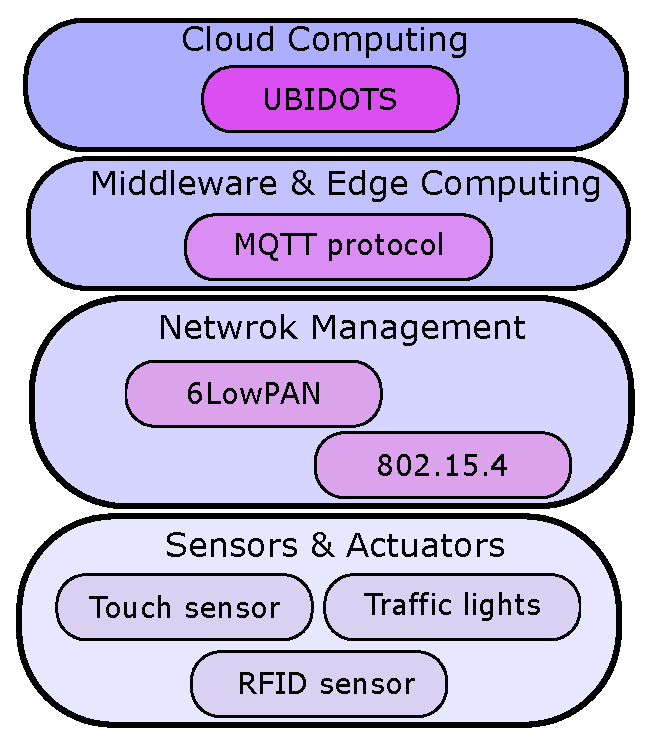
\includegraphics[width=2in]{Figures/StackIoTv1.eps}
\caption{UTLC network layers}
\label{fig:StackIoT.pdf}
\end{figure}

	\section{Results exploitation} \label{sec:Results exploitation}

% Initiation
%Below we report the results of applying the contagion process model to the Enron Email dataset.


% Final findings
%In summary,
%	results presented in this section show that if the trust coefficient between users is up to 0.8,
%	the vulnerability diffusion process through trust relationship is at its high level of speed.
%This what happens when a new information appears in a communication network and users forward it largely in the network.
%In addition,
%	this work gives a new insight to understand the relationship between trust,
%	reputation,
%	individual vulnerability and social vulnerability in the context of messaging services such as emails.


\subsection{Range}

\subsection{Response time}

\subsection{Connection speed}

\subsection{Power consumption}

	\section{Discussion} \label{sec:Conclusion}

%purpose
The purpose of the project was to find and examine a communication protocol that could be suitable for IoT applications,
	by investigating the current hardware,
	OS,
	and communication protocols and building a prototype from the selected choices.
What can be said about the investigation is that it is difficult to examine all candidates in detail;
	this means that a rough selection has to be made based on initial knowledge potentially discarding good options.
The general feeling is,
	however,
	that all of the examined candidates in this project were relevant and added valuable insights to the current technology status.
The assessment gave relevant and interesting results that improved the understanding in what IoT can be used for,
	and what further areas of investigation could be.
One of the most interesting areas of further investigation would be the RDC driver,
	as it directly affects the response time and thus also the connection speed.
Even though the power consumption was not in line with the expectations,
	the reason has been found and can be resolved.
Another conclusion is that IoT is not ready for real-time applications as the latency is much higher than expected,
	for the technologies assessed in this thesis,
	and also has a high spread.
As the latency increases for each subsequent network hop and the minimum observed latency per hop is 11ms,
	when using the always-on RDC,
	this type of communication will probably only be used for applications where response time can vary greatly,
	without affecting the functionality.
CoAP as a communication protocol shows a lot of promise when combined with 6LoWPAN and IEEE 802.15.4.
It performs well given its simplicity but has one disadvantage:
	the large overhead which comes from the MAC addressing fields in the IEEE 802.15.4 frame.
If this overhead could be reduced from the current 71\% to only 30%,
	the goodput would double.
A solution would be to use a similar mechanism as BLE where the packet size varies depending on application.
Each node also has computing time left as the MCU is more powerful  than needed for the given application;
	an improvement would be to use a less powerful MCU,
	like the ARM Cortex-M0+,
	to reduce the clock speed as suggested in the discussion.
When looking at the future-proof aspect the later suggestion is probably the better,
	as the clock then could be increased if more computing power is needed.
In the future,
	batteries will hopefully be able to store more energy,
	thus increasing the time between battery changes or reducing the battery size.


\chapter[6:''I know what to do and I go and execute'' - Usain Bolt]{Genetic Algorithm For LoRa Transmission Parameter Selection}
	\begin{abstract}

% Problem
Most traffic light's control systems in smart cities are wired and have a semi-static behavior.
They are time-based, with pre-configured pattern and expensive cameras.
% Existing solutions
Although traffic lights can communicate wirelessly with incoming vehicles,
	they are less adapted to an urban environment.
If we consider light signs as an Internet of Things (IoT) network,
	one issue is to model thoroughly the change of signs' states and the Quality of Service (QoS) of this network.
In this paper,
	we propose a new architecture of Urban Traffic Light Control based on an IoT network (IoT-UTLC).
The objective is to interconnect both roads' infrastructures and traffic lights through an IoT platform.
We designed our IoT-UTLC by selecting motes and protocols of wireless sensor network (WSN).
Message Queuing Telemetry Transport (MQTT) protocol has been integrated to manage QoS.
It enables lights to adapt remotely to any situation and smoothly interrupt traffic light's classic cycles.
Our experimental results show that the MQTT protocol is efficient when the packets rate exceeds 35\% of traffic flow,
	it reduces traffic delay up to 0.05s at 90\% of congestion.
After verification and validation of our solution using a UPPAAL model checker,
	our system has been prototyped.
Motes' functions have been implemented on Contiki OS and connected through a 6LoWPAN/IEEE 802.15.4 network.
Time-stamping messages have been performed throughout the system to evaluate the MQTT protocol with different QoS levels.
In our experiments,
	we measured the Round-trip delay time (RTT) of messages exchanged between the WSN and IoT Cloud.
The results show that MQTT decreases the RTT when the Cumulative Distributed Function (CDF) of generated messages exceeds 35\%.

\end{abstract}
	\section{Introduction} \label{sec:Introduction}




\subsection{Problem Statement}

\subsection{Background}

\subsection{Purpose (Goal)}

\subsection{Limitations}

\subsection{Method}


% The structure 
This paper is organized as follows.
Section \ref{sec:Related work} elucidates summary of related works.
% Section \ref{sec:Background} provide the required background.
In section \ref{sec:Approach}, we propose our ... to ....
Section \ref{sec:Experimentation} evaluates the performance of our ... in terms of packet delivery ratio,
	throughput,
	and power consumption.
% Our findings are presented in section \ref{sec:Results}.
Section \ref{sec:Conclusion} concludes the article and gives some ideas for future work.


% Needs by statistics: Context Current needs


% Problematic Current bad state of the research


%Challenges
The difficulty to build such system is 


%Contribution 
In this work we 

% The structure 
The article is organized as follows.
Section \ref{sec:Related work} elucidates summary of related works,
In section \ref{sec:Approach}, we propose our ... to ....
Section \ref{sec:Experimentation} evaluate the performance of our ... in terms of packet delivery ratio,
	throughput,
	and power consumption.
Section \ref{sec:Conclusions} concludes the article and gives some ideas for future work.





	\section{Related work} \label{Sec:Related_Works}

Petri nets (PNs) are widely used for traffic light modelling and control \cite{huang_modular_2014}.
In  \cite{difebbraro_trafficresponsive_2006},
	deterministic-timed Petri Nets have been used to describe signalized intersections.
Undesirable deadlock states might appear when the nets are tested for some use cases.
The authors in \cite{febbraro_using_2009} have modified PNs models including  stochastic-time for one single signalized intersection.
Dotoli and Fanti \cite{dotoli_urban_2004} have built a colored timed PN with a deterministic modular framework,
	in which parts of the system,
	and even parts of the subsystems,
	can be specified and analyzed separately.
Examples using modularity are given in Soares and Vrancken \cite{dossantossoares_modular_2012},
	in which a p-timed PN is used for the control of a traffic signal in both main road and side streets.
However,
	formal characteristics of PNs (\emph{e.g.},
	deadlock and liveliness) haven’t been discussed.
Moreover,
	PNs suffer from a lack of analysis and verification tools.
To overcome these limits of PNs,
	we propose UPPAAL timed automata for design and verification of coherent state of cross road's traffic light.
UPPAAL is a timed-based modelling software with a graphical user interface.
It is the result of the research works of two universities UPPsala University in Sweden (UPP) and AALborg University in Denmark (AAL) \cite{david_uppaal_2015}.

In \cite{Web0},
	thermal cameras and on-street wired sensors detect vehicles and pedestrians in order to adapt the cycle of traffic light control systems.
However,
	such a solution can be expensive.
In addition,
	the system uses only its local view of the environment to detect the arrival of a vehicle.
Other solutions use recent technologies such as wireless sensors devices to limit the cost of thermal cameras and reduce the time needed to deploy sensors.
In \cite{tlig_decentralized_2014} and \cite{rose_internet_2015},
	the authors propose an adaptive system based on local wireless communication between lights and vehicles.
But such a solution requires a global interconnection between all road's users and infrastructure.
This problem comes from the rigid definition of technologies' standards.
Our work is not only limited to establish WSN,
	but it is scalable to interconnect heterogeneous wireless technologies through the Internet.
The obtained WSN intends to meet multiple QoS requirements of IoT applying the MQTT protocol.
In \cite{Silva2018},
	the latency of MQTT has been evaluated by calculating the average round-trip delay between two clients located in two different continents.
However,
	the evaluation has been limited to the impact of messages' size.
In our work,
	we consider the period of generated messages,
	and we calculate the RTT delays from WSN to Cloud IoT plateform.

In \cite{huang_modular_2014} \cite{difebbraro_trafficresponsive_2006} \cite{febbraro_using_2009} \cite{dossantossoares_modular_2012},
	the authors focus only on the structural analysis of their models and the transitions between colors of traffic lights.
However,
	the implementation of their models as a service in the Internet of smart cities has not been discussed.
Moreover,
	their methodology is not tested with any real traffic lights' Testbed.

	% \section{Background} \label{sec:Background}

% \subsubsection{Hardware}

% \subsubsection{Operating system}

% \subsubsection{Communication protocol}


	\section{Proposed Framework} \label{sec:Approach}


% A generic scheme to solve the configuration selection problem and any other similar selection problem is given in this section..
% The genetic selection scheme consists of three main steps,
% 	the first step contains a set of small parallel fuzzy logic (FL)-based subsystems,
% 	the second step is a multiple criteria decision making (MCDM) system,
% 	and the third step is a genetic algorithm (GA)-based component to assign a suitable weight for the criteria in the second component.
% The scheme decision phase can be described in more detail as follows.


% \begin{figure}
% \placetextbox{0.75}{0.8}{
% 		\tiny \mywhiteblackbox{
% 		\begin{tabular}{l} 
% 			Source program \\\hline
% 	        Ada\\
% 	        C/C++\\
% 	        Java\\ 
% 		    Perl\\
% 		    Python\\
% 		    ...
% 	    \end{tabular}
% 	}
% }
% \end{figure}


% \Figure{h}{.5}{drawing.svg}{kjkjkj rd}
	% \begin{tikzpicture}
	% 	\scriptsize
	% 	% \node[draw,align=left,dashed, text width = 0.2\linewidth] at (3,6) {Criteria c1 fuzzy based control};

	% 	\node[draw,align=left,dashed, text width = .5cm, text height = .5cm] at (3,6) {Multiple criteria decision making};
	% 	\node[draw,align=left,dashed, text width = 2cm, text height = 2cm] at (6,6) {Multiple criteria decision making};
	% 	\node[draw,align=left,dashed, text width = 2cm, text height = 2cm] at (6,3) {Genetic algorithm to determine weights of criteria (w1, ..., wn)};
	% 	\draw[->,black,thick,dashed] (0,0) -- (1,1);
	% \end{tikzpicture}

% \textbf{Definition:} stopping criteria, population size P, and mutation probability pm\\
% \textbf{Generate} randomly the initial configurations \\
% \textbf{repeat:}\\
% . . . \textbf{for} each configuration do\\
% . . . . . . Train a model \& compute configuration's fitness\\
% . . . \textbf{end}\\
% . . . \textbf{for} each reproduction 1 ... P/2 do\\
% . . . . . . \textbf{Select:} 2 configurations based on fitness\\
% . . . . . . \textbf{Crossover:} Produce 2 child configurations\\
% . . . . . . \textbf{Mutate:} child configurations with pm\\
% . . . \textbf{end}\\
% \textbf{until} stopping criterion are met\\

% \State\textbf{Definition:} stopping criteria, population size P, and mutation probability pm\\
% \State\textbf{Generate} randomly the initial configurations


\begin{algorithm}
	 \KwData{QoS constraints}
	 \KwResult{Ranked configuration list}



\SetKwFunction{FMain}{Main}
\SetKwProg{GA}{GA}{:}{end}
\GA{}{
	\Repeat{stopping criterion is met}{
		\For{each configuration}{
			Train \& compute configuration's fitness
		}
		\For{each reproduction 1 ... P/2}{
			\textbf{Select:} 2 configurations based on fitness\;
			\textbf{Crossover:} Produce 2 child configurations\;
			\textbf{Mutate:} child configurations with pm\;
		}
	}
}

% \SetKwFunction{FMain}{Main}
% \SetKwProg{FL}{FL}{:}{end}
% \FL{}{
%     \eIf{$error \geq e$}{
%         Do that as well
%     }{
%         Do otherwise
%     }
%     \While{$something \not= 0$ }{	
%         $var1 \leftarrow var2$  	
%     }

% }
% \eIf{understand}{
%   go to next section\;
%   current section becomes this one\;
% }{
%   go back to the beginning of current section\;
% }

\caption{LoRa Transmission Parameter Selection}
\end{algorithm}
\medskip

The scheme selection process can be described following these five steps:

\begin{enumerate}
	\item According to the Semtech SX1276 specification\cite{lorasemtech}, there is 6720 possible settings ($s_{1}$, ... ,$s_{6720}$) and the framework has to select the most optimal one or to rank them according to their relevance.
	\item The first step of the selection process depends on multiple criteria up to i ($c_{1}$, ... , $c_{i}$).
		Different type of criteria can be measured from different sources to cover the maximum point of views,
		as example,
		the network server requirements, the applications requirements and the devices conditions.
	\item The Fuzzy Logic (FL) based subsystem gives an initial score for each configuration that reflects its relevance.
		The different sets of scores ($d_{1}$, ... ,$d_{i}$) are sent to the \ac{MCDM} in the $5^{th}$ step.
	\item At the same time,
			the genetic algorithm (GA) \cite{alkhawlani_access_2008} assigns a suitable weight ($w_{1}$, ... ,$w_{i}$) for each initial selection decision according to the objective function that is required by the application.
			% according to the importance and sensitivities of ANS criteria to the different characteristics of a wireless heterogeneous environment.
	\item Using the initial scores coming from the $3^{rd}$ step and the weights that are assigned using the $4^{th}$ step,
			the multi criteria decision making{} \ac{MCDM} will select the most relevant settings and rank them according to their reward.
\end{enumerate}


\Figure{h}{1}{genetic}{The proposed scheme for LoRa transmission parameters selection based on \ac{GA}, \ac{FL} and \ac{MCDM}}

	\section{Prototyping} \label{sec:Experimentation}

% Intro
We have prototyped the wireless sensors and actuator's network of traffic lights and roads on a mockup \footnote{https://github.com/IoT-UTLC/Resources/wiki} of real intersection in Paris with a scale of 1:68.
Our specifications have been defined considering the low-cost and energy efficiency of the solution.
This Testbed is a proof of concept of not limited to our use case as it is scalable for other applications.
For example,
	additional sensors of fine particules could be implanted bringing correlation between traffic jam and pollution.

\begin{figure*}[!htb]
\centering
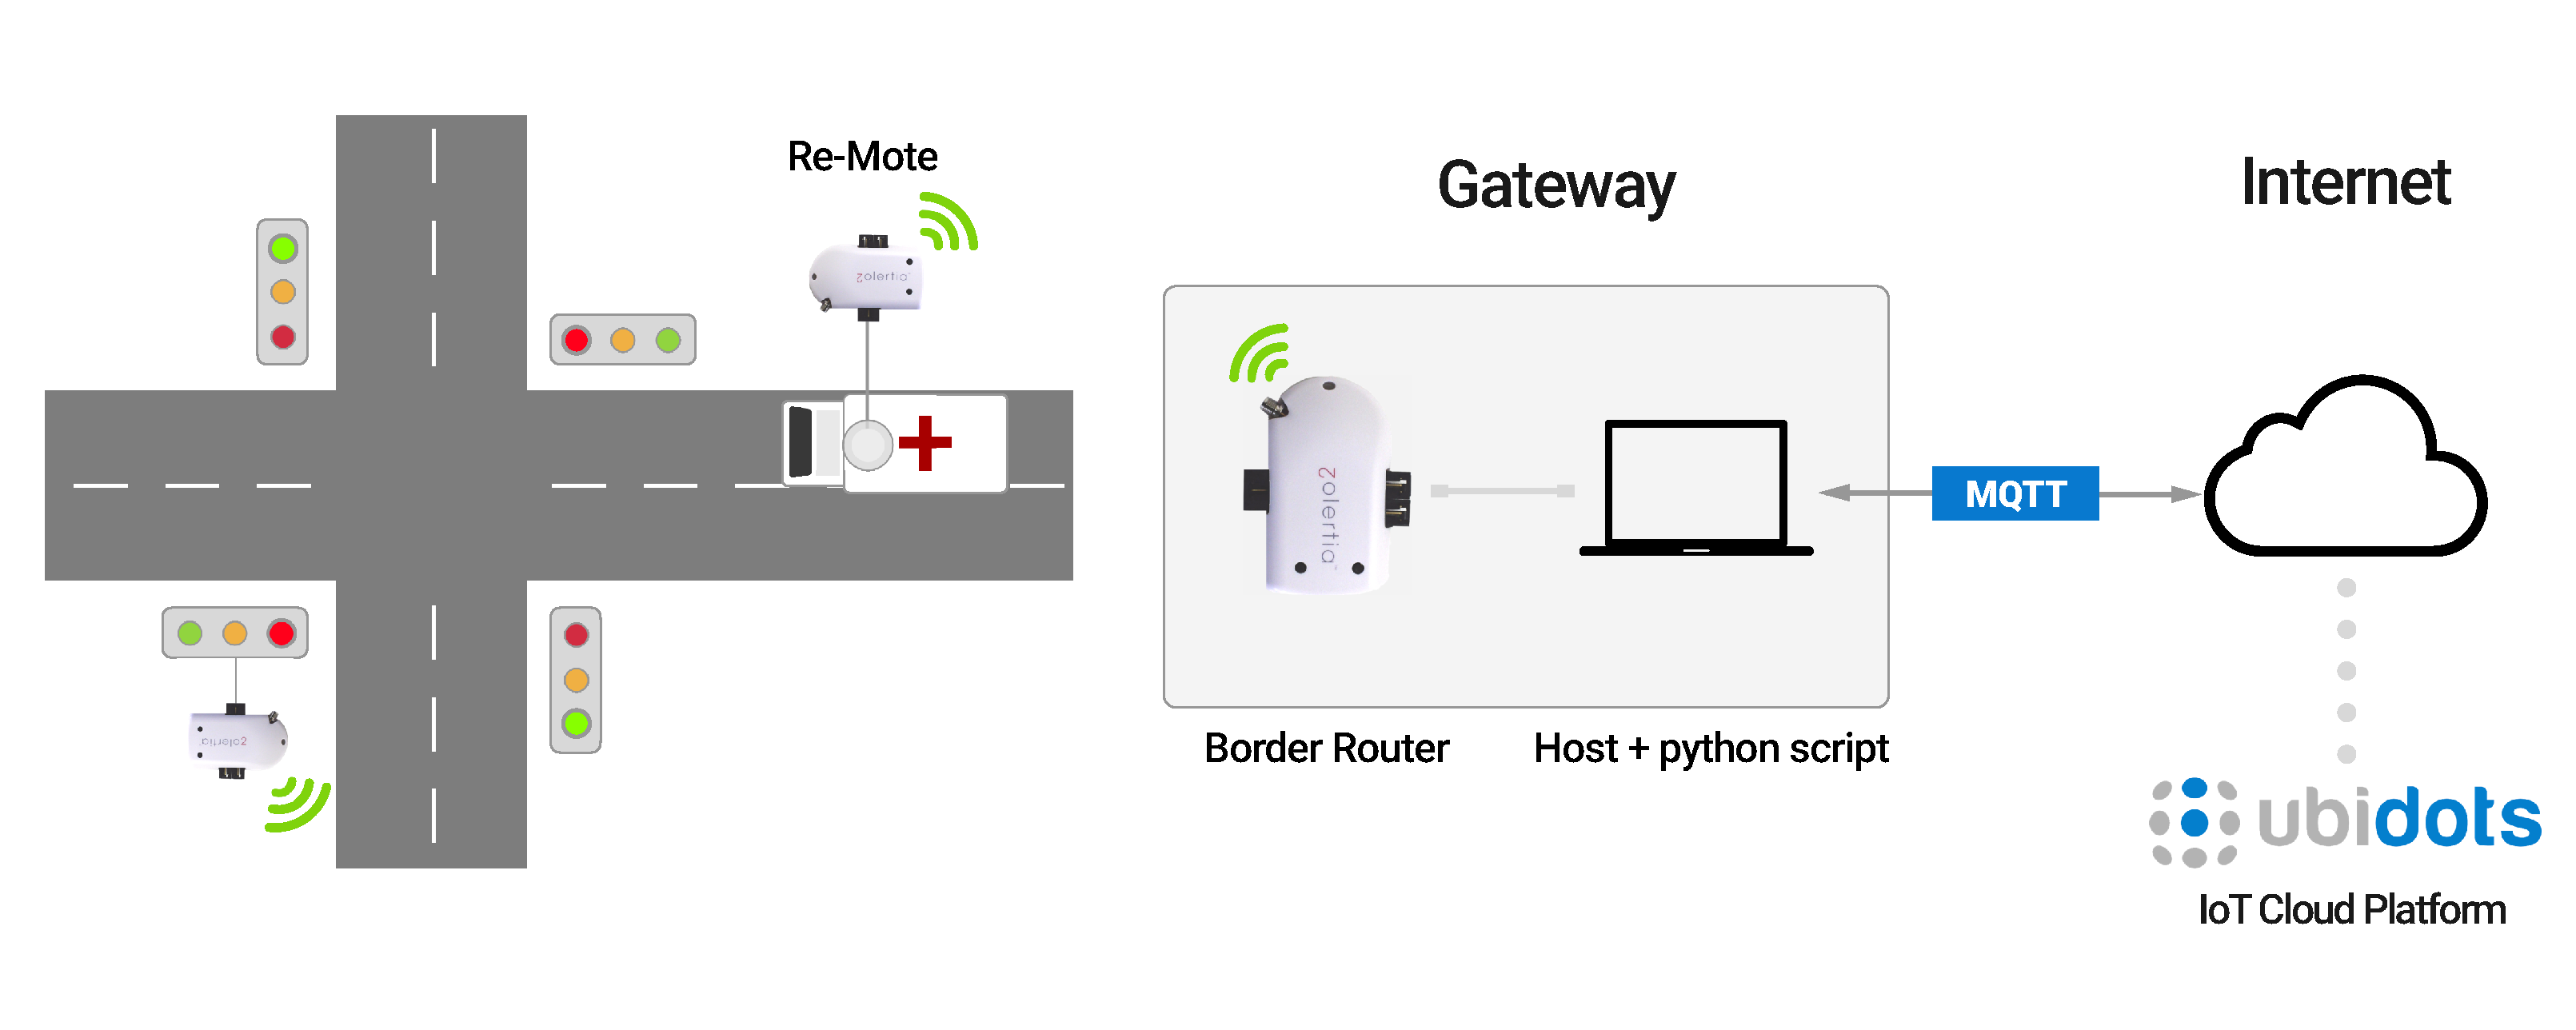
\includegraphics[width=4.5in]{Figures/ScenarioPaper.eps}
\caption{Architecture of  Iot-UTLC}
\label{fig:ScenarioPaper.eps}
\end{figure*}

Fig.
\ref{fig:ScenarioPaper.eps} shows the architecture of our IoT-UTLC with three layers.
From left to right,
	we have the WSN layer with connected traffic lights’ actuators,
	sensors and IEEE 802.15.4 transceivers.
The second part is the gateway of the WSN ensured by the BR and the Middleware \emph{i.e.} Python script launched by host computer.
The last layer is the Ubidots IoT Cloud Platform.
It is an open source solution used to collect and analyze WSN data.

\subsection{6LoWPAN, Contiki OS, Re-Mote and Border Router} \label{Sec:Contiki}

% 6LoWPAN
Our WSN is an IPv6 LowPower Wireless Personal Area Network (6LoWPAN) based on IEEE 802.15.4 stack.
It is well adapted to embedded wireless devices with energy aware constraint and for its capabilities to define a mesh topology.
Contiki Os\footnote{http://www.contiki-os.org/} has been used to implement networks' functions such as send,
	receive and data processing.
It is an embedded operating system with large open source community.
It supports Zolertia's Re-Motes \footnote{https://github.com/Zolertia/Resources/wiki/RE-Mote} and implements recent IEEE 802.15.4 standard specifications.
It also includes protocols such as RPL,
	CoAP and MQTT.
Furthermore,
	developer community is active and makes available source codes examples in order to help developing quickly new applications.

% Re-motes
Re-motes are compatible with our WSN specifications and our design model.
They are wireless devices with ultra-low power operation mode.
This choice has been motivated by long radio range of its IEEE 802.15.4 CC1200 transceiver,
	which transmits in the frequency band of 868-915 MHz.
In addition,
	each Re-Mote has analog and digital ports with a possibility to connect several analog sensors and actuators.
A Re-mote can be driven by a computer and become a sink and/or BR as well as a gateway between the 6LoWPAN network and the computer.

%\Figure{!htb}{1}{ethernetRouter.png}{Our Ethernet router}
\begin{figure}[!htb]
\centering
\includegraphics[width=2.5in]{Figures/ethernetRouter.png}
\caption{BR and sink combined on one board}
\label{fig:ethernetRouter.png}
\end{figure}

%[Explanation of how it works with the 2 radios,
To implement the previous model described in Section \ref{sec:Use Case and Model Design},
	we used six Re-motes:
	one for the BR,
	four to control the traffic lights and one Re-Mote to detect the arrival of a high priority vehicle near a crossing point.
For simplicity,
	we choose a touch sensor as a detecting device of priority vehicle.
We have developed four types of programs running on a Re-mote:
	traffic lights signs,
	sensors,
	high priority vehicle detecting device and BR function.
Sensors send periodically information to the IoT Cloud Platform with temperature,
	pressure or any relevant information that can be sensed.
As mentioned in the previous section,
	traffic lights are sub-divided into two modes:
	slaves and masters.
Masters nodes are the only ones to request the Middleware to change its light’s state and slaves simply change its state depending on received packets.
These roles are defined to reduce the overhead of network,
	redundancy and collisions,
	for instance.
Masters send periodically packets to request a change of state to the Middleware which forwards them to a Cloud platform.
 
BR node behaves differently compared to the other Re-motes.
The entries of its routing table are the list of Re-motes that pass through it.
It reroutes every packet it receives from its neighboring to host computer (or sink),
	which  creates a connection to the IoT Cloud platform.
Two options are possible to create our BR:
	i) separate the BR and sink and ii) combine both on the same device.
In our development,
	we worked on how to implement the sink and the BR nodes on the same Re-Mote board.
Fig.
\ref{fig:ethernetRouter.png} shows a prototype of the combined BR and sink,
	both connected to an ethernet interface.
Indeed,
	if the border router becomes an Ethernet router,
	there will no longer be any connection between the host/sink machine and the IoT Cloud platform.
Every Re-mote is able to connect independently to the IoT Cloud platform.
This approach has some advantages,
	such as the autonomy of the devices,
	but it generates an overhead requiring extra synchronization packets' exchange.
Therefore,
	we separate the sink and BR,
	since this solution is more flexible and resilient for our Testbed.

%The border router is at first a Re-mote,
%	but it has very different behavior and function.
%Indeed it has the task of re-routing every packet it receives from its cohorts to the serial port of the host machine.


%This machine will create a connection to the IoT Cloud platform and send the Re-motes messages to it and get responses for the Re-motes.
%The border router is a central node because it knows all to Re-motes in the 6LoWPAN which packets have transited by it.
%It acts as a Router and has a routing table of those Re-motes that pass through it.
%A web server page can be accessed to retrieve that information.
%We also tried a different approach of it.

 % [
%Transition with next paragraph => the use of MQTT to access the other "side" of the system
%Explanation of how it works (encapsulating the headers ...)
%]
%[
%Big part of how it works,
%what is good about it %New paragraph about the autonomous BR we were trying to develop
%Comparison between the 2 solutions
%]

% Autonomous BR
%As we have seen before,
%	this approach requires a Border Router linked the computer itself to the internet,
%	we tried to see if we can remove one part.
%Thus,
%	we added a component to the Re-mote in order to connect it directly to the internet via an Ethernet cable.

%[Transition with next paragraph => the use of MQTT to access the other "side" of the system]

\subsection{MQTT and UBIDOTS} \label{Sec:MQTT}

Fig.
\ref{fig:StackIoT.pdf} presents the layers of our UTLC network.
From bottom to up,
	the WSN network sense and/or detect,
	process and actuates traffic lights.
The second layer manages the 6 LowPan addressing and routing of packets throughout an IEEE 802.15.4 network.
The Edge Computing is the Middleware between the WSN and the Cloud platform.
For the setup of our UTLC,
	we start by establishing the access network of WSN.
The next step is to connect this network to Core network.
MQTT protocol controls three levels of QoS of exchanged packets from the WSN to the chosen Ubidots \footnote{https://ubidots.com/} Cloud platform.
It adopts IntServ approach for supporting quality of service in the network,
	it tags incoming packets in the border routers with different levels of priority.
Core routers read incoming packets headers and queue them according to their priority,
	packets with a high priority are sent faster compared to low priority ones.

MQTT ensures the QoS and publish/subscribe mechanisms through a broker.
The broker behaves as a server by filtering messages and organizing them in topics,
	which are strings used to filter messages and define the hierarchy of our data structure.
They allow us to organize how to receive multiple data from sensors such as temperature,
	up time,
	battery status and how to display them and obtain a real-time glance of our system.
It gets its messages from publishers and sends any modifications to entities,
	which that subscribed to the updated topics.
We used this mechanism with the Middleware in order to publish messages to the broker and get from the main topic the new values of the subscriber.

%We have seen in previous section what we used for our local sensors network, let's see now how we communicate with the IoT Cloud Platform. We will use MQTT which is a light-weight transportation protocol. In our solution, a python script will run an MQTT client to connect our WSN to Ubidots.

%MQTT ensures the QoS and publishes/subscribes mechanisms with a noteworthy topic organization. 

%The topics are strings used to filter messages and define the hierarchy of our data structure. They allow us to organize how to receive multiple data from sensors such as temperature, up time, battery status and how to display them and obtain a real-time glance of our system. 

%In addition, the broker behaves as a server by filtering messages and organize them in topics. It gets its messages from publishers and will send any modifications to entities which would have subscribed to the updated topics. We used this mechanism with the middleware in order to publish messages to the broker and get from the main topic the new values using the subscriber functionality.


The QoS feature of MQTT protocol manages network resources by handling retransmissions and guarantees the delivery of messages. It allows more control on messages by defining the level of guarantee. By default, the QoS is defined by three levels. The first one, level 0, is `At most one`. Level 1 is `At least one` where there is an acknowledgment to let the sender know that its packet has been received. Finally, level 2 `Exactly once` is the highest verification level with a request/response flows to ensure that only one message will be delivered and processed by the receiver. In our case, we applied levels 1 and 2 using \textit{paho.mqtt.client} Python library.  
%
%For example, subscribed clients could define the data QoS level of requested data by the source code shown bellow. 
For example, publisher of high priority data such as touch sensor has to indicate the highest level of QoS by the code shown bellow. 
We shared our implementation and its source codes at https://github.com/IoT-UTLC/contiki.
%
%\begin{footnotesize}
%\begin{lstlisting}
%# client receives a CONNACK response 
%# from the server.
%def on_connect(client, userdata, flags, rc):
%  print("Subscribed to " + MQTT_URL_TOPIC)
%  client.subscribe(MQTT_URL_TOPIC, 2) 
%  # 2nd arg is the QoS level to use 
%  # at maximum when it's needed
%\end{lstlisting}
%\end{footnotesize}

\begin{footnotesize}
\begin{lstlisting}
payload = json.dumps({"RoadA": data, "RoadB": 0})
res, mid = conn.publish(MQTT_URL_PUB, payload,
	  qos=int(QoS)) # QoS is QoS level to use 
\end{lstlisting}
\end{footnotesize}


%# The callback for when the client receives a CONNACK response from the server.
%def on_connect(client, userdata, flags, rc):
%	print("Connected with result code "+str(rc))
%	print("Subscribed to " + MQTT_URL_TOPIC)
%	client.subscribe(MQTT_URL_TOPIC, 2) 
                                                                                                                                                        
We experienced significant latency of high priority messages when we tested of IoT-UTLC mockup. Therefore, assessments of the MQTT protocol in our case provided significant information about its efficiency. 

%  For the end point the IoT Cloud platform,
% we wanted to be simple  %QoS and MQTT resilient by default (good implementation)
% Get relevant information from dashboard
% Access from anywhere (remote control possible)
% Structure our system / hierarchy
%
%As for the MQTT broker, we wanted an easy and powerful IoT Cloud Platform.
%It will be compatible with all technologies we chose for our prototyping,
%	so with an integration of MQTT and QoS levels.
%an IoT Cloud platform is a central point of the system as it keeps all the information about our WSN.
%Using the Cloud allows the system being accessible from anywhere on the internet.
%It is also a tool to filter and display relevant information in real-time from our system in the centralized dashboard.
%It can be possible to trigger some actions on the system via the dashboard.
%
%% Architecture
%Building this virtual infrastructure for this project has been challenging.
%we used MQTT topics mechanism to get the most of Ubidots to structure every data sent.
%We have a main topic which contains the states of the traffic light (RoadA and RoadB) in real time,
%	we created individual topics for every Re-mote acting as traffic lights or sensors.
%With this architecture,
%	we can have deep information on every device (such as its battery,
%	sensors data,
%	etc...).
%Moreover,
%	it could be scaled to match future needs.


%\Figure{!htb}{1}{cdf_distribution.pdf}{Normal,Gamma and Logistic distribution}
\begin{figure}[!htb]
\centering
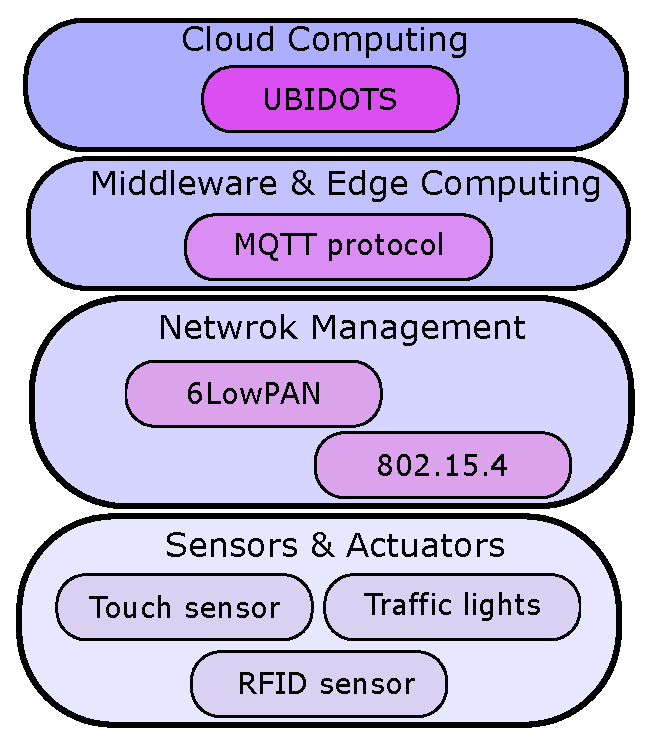
\includegraphics[width=2in]{Figures/StackIoTv1.eps}
\caption{UTLC network layers}
\label{fig:StackIoT.pdf}
\end{figure}

	% \section{Results exploitation} \label{sec:Results exploitation}

% Initiation
%Below we report the results of applying the contagion process model to the Enron Email dataset.


% Final findings
%In summary,
%	results presented in this section show that if the trust coefficient between users is up to 0.8,
%	the vulnerability diffusion process through trust relationship is at its high level of speed.
%This what happens when a new information appears in a communication network and users forward it largely in the network.
%In addition,
%	this work gives a new insight to understand the relationship between trust,
%	reputation,
%	individual vulnerability and social vulnerability in the context of messaging services such as emails.


\subsection{Range}

\subsection{Response time}

\subsection{Connection speed}

\subsection{Power consumption}

	\section{Discussion} \label{sec:Conclusion}

%purpose
The purpose of the project was to find and examine a communication protocol that could be suitable for IoT applications,
	by investigating the current hardware,
	OS,
	and communication protocols and building a prototype from the selected choices.
What can be said about the investigation is that it is difficult to examine all candidates in detail;
	this means that a rough selection has to be made based on initial knowledge potentially discarding good options.
The general feeling is,
	however,
	that all of the examined candidates in this project were relevant and added valuable insights to the current technology status.
The assessment gave relevant and interesting results that improved the understanding in what IoT can be used for,
	and what further areas of investigation could be.
One of the most interesting areas of further investigation would be the RDC driver,
	as it directly affects the response time and thus also the connection speed.
Even though the power consumption was not in line with the expectations,
	the reason has been found and can be resolved.
Another conclusion is that IoT is not ready for real-time applications as the latency is much higher than expected,
	for the technologies assessed in this thesis,
	and also has a high spread.
As the latency increases for each subsequent network hop and the minimum observed latency per hop is 11ms,
	when using the always-on RDC,
	this type of communication will probably only be used for applications where response time can vary greatly,
	without affecting the functionality.
CoAP as a communication protocol shows a lot of promise when combined with 6LoWPAN and IEEE 802.15.4.
It performs well given its simplicity but has one disadvantage:
	the large overhead which comes from the MAC addressing fields in the IEEE 802.15.4 frame.
If this overhead could be reduced from the current 71\% to only 30%,
	the goodput would double.
A solution would be to use a similar mechanism as BLE where the packet size varies depending on application.
Each node also has computing time left as the MCU is more powerful  than needed for the given application;
	an improvement would be to use a less powerful MCU,
	like the ARM Cortex-M0+,
	to reduce the clock speed as suggested in the discussion.
When looking at the future-proof aspect the later suggestion is probably the better,
	as the clock then could be increased if more computing power is needed.
In the future,
	batteries will hopefully be able to store more energy,
	thus increasing the time between battery changes or reducing the battery size.


\chapter[7:''la patience fait fondre le marbre'' -- Amer]{Template}
	\begin{abstract}

% Problem
Most traffic light's control systems in smart cities are wired and have a semi-static behavior.
They are time-based, with pre-configured pattern and expensive cameras.
% Existing solutions
Although traffic lights can communicate wirelessly with incoming vehicles,
	they are less adapted to an urban environment.
If we consider light signs as an Internet of Things (IoT) network,
	one issue is to model thoroughly the change of signs' states and the Quality of Service (QoS) of this network.
In this paper,
	we propose a new architecture of Urban Traffic Light Control based on an IoT network (IoT-UTLC).
The objective is to interconnect both roads' infrastructures and traffic lights through an IoT platform.
We designed our IoT-UTLC by selecting motes and protocols of wireless sensor network (WSN).
Message Queuing Telemetry Transport (MQTT) protocol has been integrated to manage QoS.
It enables lights to adapt remotely to any situation and smoothly interrupt traffic light's classic cycles.
Our experimental results show that the MQTT protocol is efficient when the packets rate exceeds 35\% of traffic flow,
	it reduces traffic delay up to 0.05s at 90\% of congestion.
After verification and validation of our solution using a UPPAAL model checker,
	our system has been prototyped.
Motes' functions have been implemented on Contiki OS and connected through a 6LoWPAN/IEEE 802.15.4 network.
Time-stamping messages have been performed throughout the system to evaluate the MQTT protocol with different QoS levels.
In our experiments,
	we measured the Round-trip delay time (RTT) of messages exchanged between the WSN and IoT Cloud.
The results show that MQTT decreases the RTT when the Cumulative Distributed Function (CDF) of generated messages exceeds 35\%.

\end{abstract}
	\section{Introduction} \label{sec:Introduction}




\subsection{Problem Statement}

\subsection{Background}

\subsection{Purpose (Goal)}

\subsection{Limitations}

\subsection{Method}


% The structure 
This paper is organized as follows.
Section \ref{sec:Related work} elucidates summary of related works.
% Section \ref{sec:Background} provide the required background.
In section \ref{sec:Approach}, we propose our ... to ....
Section \ref{sec:Experimentation} evaluates the performance of our ... in terms of packet delivery ratio,
	throughput,
	and power consumption.
% Our findings are presented in section \ref{sec:Results}.
Section \ref{sec:Conclusion} concludes the article and gives some ideas for future work.


% Needs by statistics: Context Current needs


% Problematic Current bad state of the research


%Challenges
The difficulty to build such system is 


%Contribution 
In this work we 

% The structure 
The article is organized as follows.
Section \ref{sec:Related work} elucidates summary of related works,
In section \ref{sec:Approach}, we propose our ... to ....
Section \ref{sec:Experimentation} evaluate the performance of our ... in terms of packet delivery ratio,
	throughput,
	and power consumption.
Section \ref{sec:Conclusions} concludes the article and gives some ideas for future work.





	\section{Related work} \label{Sec:Related_Works}

Petri nets (PNs) are widely used for traffic light modelling and control \cite{huang_modular_2014}.
In  \cite{difebbraro_trafficresponsive_2006},
	deterministic-timed Petri Nets have been used to describe signalized intersections.
Undesirable deadlock states might appear when the nets are tested for some use cases.
The authors in \cite{febbraro_using_2009} have modified PNs models including  stochastic-time for one single signalized intersection.
Dotoli and Fanti \cite{dotoli_urban_2004} have built a colored timed PN with a deterministic modular framework,
	in which parts of the system,
	and even parts of the subsystems,
	can be specified and analyzed separately.
Examples using modularity are given in Soares and Vrancken \cite{dossantossoares_modular_2012},
	in which a p-timed PN is used for the control of a traffic signal in both main road and side streets.
However,
	formal characteristics of PNs (\emph{e.g.},
	deadlock and liveliness) haven’t been discussed.
Moreover,
	PNs suffer from a lack of analysis and verification tools.
To overcome these limits of PNs,
	we propose UPPAAL timed automata for design and verification of coherent state of cross road's traffic light.
UPPAAL is a timed-based modelling software with a graphical user interface.
It is the result of the research works of two universities UPPsala University in Sweden (UPP) and AALborg University in Denmark (AAL) \cite{david_uppaal_2015}.

In \cite{Web0},
	thermal cameras and on-street wired sensors detect vehicles and pedestrians in order to adapt the cycle of traffic light control systems.
However,
	such a solution can be expensive.
In addition,
	the system uses only its local view of the environment to detect the arrival of a vehicle.
Other solutions use recent technologies such as wireless sensors devices to limit the cost of thermal cameras and reduce the time needed to deploy sensors.
In \cite{tlig_decentralized_2014} and \cite{rose_internet_2015},
	the authors propose an adaptive system based on local wireless communication between lights and vehicles.
But such a solution requires a global interconnection between all road's users and infrastructure.
This problem comes from the rigid definition of technologies' standards.
Our work is not only limited to establish WSN,
	but it is scalable to interconnect heterogeneous wireless technologies through the Internet.
The obtained WSN intends to meet multiple QoS requirements of IoT applying the MQTT protocol.
In \cite{Silva2018},
	the latency of MQTT has been evaluated by calculating the average round-trip delay between two clients located in two different continents.
However,
	the evaluation has been limited to the impact of messages' size.
In our work,
	we consider the period of generated messages,
	and we calculate the RTT delays from WSN to Cloud IoT plateform.

In \cite{huang_modular_2014} \cite{difebbraro_trafficresponsive_2006} \cite{febbraro_using_2009} \cite{dossantossoares_modular_2012},
	the authors focus only on the structural analysis of their models and the transitions between colors of traffic lights.
However,
	the implementation of their models as a service in the Internet of smart cities has not been discussed.
Moreover,
	their methodology is not tested with any real traffic lights' Testbed.

	% \section{Background} \label{sec:Background}

% \subsubsection{Hardware}

% \subsubsection{Operating system}

% \subsubsection{Communication protocol}


	\section{Proposed Framework} \label{sec:Approach}


% A generic scheme to solve the configuration selection problem and any other similar selection problem is given in this section..
% The genetic selection scheme consists of three main steps,
% 	the first step contains a set of small parallel fuzzy logic (FL)-based subsystems,
% 	the second step is a multiple criteria decision making (MCDM) system,
% 	and the third step is a genetic algorithm (GA)-based component to assign a suitable weight for the criteria in the second component.
% The scheme decision phase can be described in more detail as follows.


% \begin{figure}
% \placetextbox{0.75}{0.8}{
% 		\tiny \mywhiteblackbox{
% 		\begin{tabular}{l} 
% 			Source program \\\hline
% 	        Ada\\
% 	        C/C++\\
% 	        Java\\ 
% 		    Perl\\
% 		    Python\\
% 		    ...
% 	    \end{tabular}
% 	}
% }
% \end{figure}


% \Figure{h}{.5}{drawing.svg}{kjkjkj rd}
	% \begin{tikzpicture}
	% 	\scriptsize
	% 	% \node[draw,align=left,dashed, text width = 0.2\linewidth] at (3,6) {Criteria c1 fuzzy based control};

	% 	\node[draw,align=left,dashed, text width = .5cm, text height = .5cm] at (3,6) {Multiple criteria decision making};
	% 	\node[draw,align=left,dashed, text width = 2cm, text height = 2cm] at (6,6) {Multiple criteria decision making};
	% 	\node[draw,align=left,dashed, text width = 2cm, text height = 2cm] at (6,3) {Genetic algorithm to determine weights of criteria (w1, ..., wn)};
	% 	\draw[->,black,thick,dashed] (0,0) -- (1,1);
	% \end{tikzpicture}

% \textbf{Definition:} stopping criteria, population size P, and mutation probability pm\\
% \textbf{Generate} randomly the initial configurations \\
% \textbf{repeat:}\\
% . . . \textbf{for} each configuration do\\
% . . . . . . Train a model \& compute configuration's fitness\\
% . . . \textbf{end}\\
% . . . \textbf{for} each reproduction 1 ... P/2 do\\
% . . . . . . \textbf{Select:} 2 configurations based on fitness\\
% . . . . . . \textbf{Crossover:} Produce 2 child configurations\\
% . . . . . . \textbf{Mutate:} child configurations with pm\\
% . . . \textbf{end}\\
% \textbf{until} stopping criterion are met\\

% \State\textbf{Definition:} stopping criteria, population size P, and mutation probability pm\\
% \State\textbf{Generate} randomly the initial configurations


\begin{algorithm}
	 \KwData{QoS constraints}
	 \KwResult{Ranked configuration list}



\SetKwFunction{FMain}{Main}
\SetKwProg{GA}{GA}{:}{end}
\GA{}{
	\Repeat{stopping criterion is met}{
		\For{each configuration}{
			Train \& compute configuration's fitness
		}
		\For{each reproduction 1 ... P/2}{
			\textbf{Select:} 2 configurations based on fitness\;
			\textbf{Crossover:} Produce 2 child configurations\;
			\textbf{Mutate:} child configurations with pm\;
		}
	}
}

% \SetKwFunction{FMain}{Main}
% \SetKwProg{FL}{FL}{:}{end}
% \FL{}{
%     \eIf{$error \geq e$}{
%         Do that as well
%     }{
%         Do otherwise
%     }
%     \While{$something \not= 0$ }{	
%         $var1 \leftarrow var2$  	
%     }

% }
% \eIf{understand}{
%   go to next section\;
%   current section becomes this one\;
% }{
%   go back to the beginning of current section\;
% }

\caption{LoRa Transmission Parameter Selection}
\end{algorithm}
\medskip

The scheme selection process can be described following these five steps:

\begin{enumerate}
	\item According to the Semtech SX1276 specification\cite{lorasemtech}, there is 6720 possible settings ($s_{1}$, ... ,$s_{6720}$) and the framework has to select the most optimal one or to rank them according to their relevance.
	\item The first step of the selection process depends on multiple criteria up to i ($c_{1}$, ... , $c_{i}$).
		Different type of criteria can be measured from different sources to cover the maximum point of views,
		as example,
		the network server requirements, the applications requirements and the devices conditions.
	\item The Fuzzy Logic (FL) based subsystem gives an initial score for each configuration that reflects its relevance.
		The different sets of scores ($d_{1}$, ... ,$d_{i}$) are sent to the \ac{MCDM} in the $5^{th}$ step.
	\item At the same time,
			the genetic algorithm (GA) \cite{alkhawlani_access_2008} assigns a suitable weight ($w_{1}$, ... ,$w_{i}$) for each initial selection decision according to the objective function that is required by the application.
			% according to the importance and sensitivities of ANS criteria to the different characteristics of a wireless heterogeneous environment.
	\item Using the initial scores coming from the $3^{rd}$ step and the weights that are assigned using the $4^{th}$ step,
			the multi criteria decision making{} \ac{MCDM} will select the most relevant settings and rank them according to their reward.
\end{enumerate}


\Figure{h}{1}{genetic}{The proposed scheme for LoRa transmission parameters selection based on \ac{GA}, \ac{FL} and \ac{MCDM}}

	\section{Prototyping} \label{sec:Experimentation}

% Intro
We have prototyped the wireless sensors and actuator's network of traffic lights and roads on a mockup \footnote{https://github.com/IoT-UTLC/Resources/wiki} of real intersection in Paris with a scale of 1:68.
Our specifications have been defined considering the low-cost and energy efficiency of the solution.
This Testbed is a proof of concept of not limited to our use case as it is scalable for other applications.
For example,
	additional sensors of fine particules could be implanted bringing correlation between traffic jam and pollution.

\begin{figure*}[!htb]
\centering
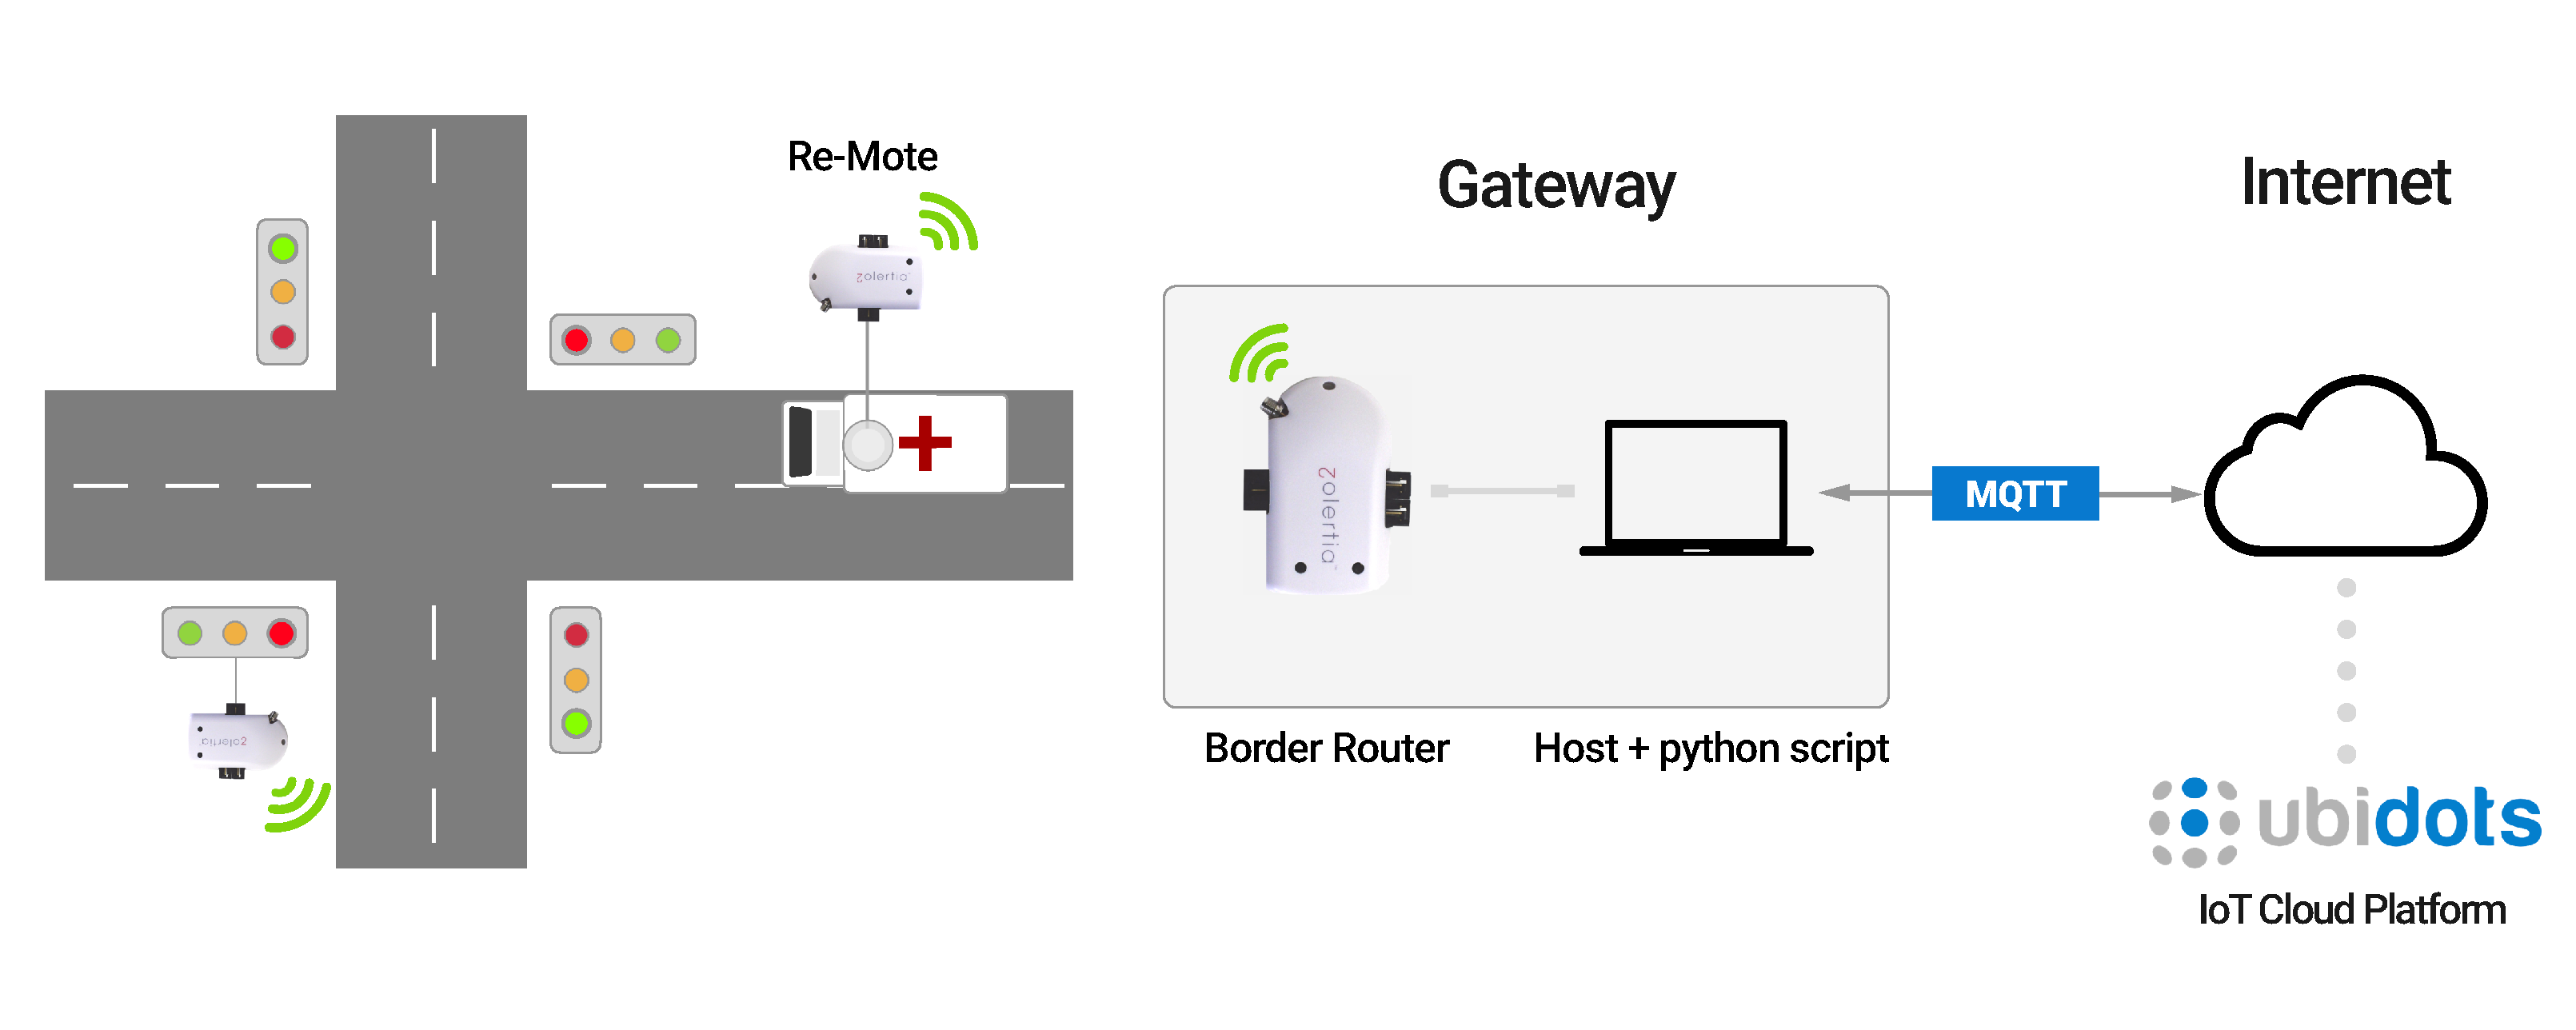
\includegraphics[width=4.5in]{Figures/ScenarioPaper.eps}
\caption{Architecture of  Iot-UTLC}
\label{fig:ScenarioPaper.eps}
\end{figure*}

Fig.
\ref{fig:ScenarioPaper.eps} shows the architecture of our IoT-UTLC with three layers.
From left to right,
	we have the WSN layer with connected traffic lights’ actuators,
	sensors and IEEE 802.15.4 transceivers.
The second part is the gateway of the WSN ensured by the BR and the Middleware \emph{i.e.} Python script launched by host computer.
The last layer is the Ubidots IoT Cloud Platform.
It is an open source solution used to collect and analyze WSN data.

\subsection{6LoWPAN, Contiki OS, Re-Mote and Border Router} \label{Sec:Contiki}

% 6LoWPAN
Our WSN is an IPv6 LowPower Wireless Personal Area Network (6LoWPAN) based on IEEE 802.15.4 stack.
It is well adapted to embedded wireless devices with energy aware constraint and for its capabilities to define a mesh topology.
Contiki Os\footnote{http://www.contiki-os.org/} has been used to implement networks' functions such as send,
	receive and data processing.
It is an embedded operating system with large open source community.
It supports Zolertia's Re-Motes \footnote{https://github.com/Zolertia/Resources/wiki/RE-Mote} and implements recent IEEE 802.15.4 standard specifications.
It also includes protocols such as RPL,
	CoAP and MQTT.
Furthermore,
	developer community is active and makes available source codes examples in order to help developing quickly new applications.

% Re-motes
Re-motes are compatible with our WSN specifications and our design model.
They are wireless devices with ultra-low power operation mode.
This choice has been motivated by long radio range of its IEEE 802.15.4 CC1200 transceiver,
	which transmits in the frequency band of 868-915 MHz.
In addition,
	each Re-Mote has analog and digital ports with a possibility to connect several analog sensors and actuators.
A Re-mote can be driven by a computer and become a sink and/or BR as well as a gateway between the 6LoWPAN network and the computer.

%\Figure{!htb}{1}{ethernetRouter.png}{Our Ethernet router}
\begin{figure}[!htb]
\centering
\includegraphics[width=2.5in]{Figures/ethernetRouter.png}
\caption{BR and sink combined on one board}
\label{fig:ethernetRouter.png}
\end{figure}

%[Explanation of how it works with the 2 radios,
To implement the previous model described in Section \ref{sec:Use Case and Model Design},
	we used six Re-motes:
	one for the BR,
	four to control the traffic lights and one Re-Mote to detect the arrival of a high priority vehicle near a crossing point.
For simplicity,
	we choose a touch sensor as a detecting device of priority vehicle.
We have developed four types of programs running on a Re-mote:
	traffic lights signs,
	sensors,
	high priority vehicle detecting device and BR function.
Sensors send periodically information to the IoT Cloud Platform with temperature,
	pressure or any relevant information that can be sensed.
As mentioned in the previous section,
	traffic lights are sub-divided into two modes:
	slaves and masters.
Masters nodes are the only ones to request the Middleware to change its light’s state and slaves simply change its state depending on received packets.
These roles are defined to reduce the overhead of network,
	redundancy and collisions,
	for instance.
Masters send periodically packets to request a change of state to the Middleware which forwards them to a Cloud platform.
 
BR node behaves differently compared to the other Re-motes.
The entries of its routing table are the list of Re-motes that pass through it.
It reroutes every packet it receives from its neighboring to host computer (or sink),
	which  creates a connection to the IoT Cloud platform.
Two options are possible to create our BR:
	i) separate the BR and sink and ii) combine both on the same device.
In our development,
	we worked on how to implement the sink and the BR nodes on the same Re-Mote board.
Fig.
\ref{fig:ethernetRouter.png} shows a prototype of the combined BR and sink,
	both connected to an ethernet interface.
Indeed,
	if the border router becomes an Ethernet router,
	there will no longer be any connection between the host/sink machine and the IoT Cloud platform.
Every Re-mote is able to connect independently to the IoT Cloud platform.
This approach has some advantages,
	such as the autonomy of the devices,
	but it generates an overhead requiring extra synchronization packets' exchange.
Therefore,
	we separate the sink and BR,
	since this solution is more flexible and resilient for our Testbed.

%The border router is at first a Re-mote,
%	but it has very different behavior and function.
%Indeed it has the task of re-routing every packet it receives from its cohorts to the serial port of the host machine.


%This machine will create a connection to the IoT Cloud platform and send the Re-motes messages to it and get responses for the Re-motes.
%The border router is a central node because it knows all to Re-motes in the 6LoWPAN which packets have transited by it.
%It acts as a Router and has a routing table of those Re-motes that pass through it.
%A web server page can be accessed to retrieve that information.
%We also tried a different approach of it.

 % [
%Transition with next paragraph => the use of MQTT to access the other "side" of the system
%Explanation of how it works (encapsulating the headers ...)
%]
%[
%Big part of how it works,
%what is good about it %New paragraph about the autonomous BR we were trying to develop
%Comparison between the 2 solutions
%]

% Autonomous BR
%As we have seen before,
%	this approach requires a Border Router linked the computer itself to the internet,
%	we tried to see if we can remove one part.
%Thus,
%	we added a component to the Re-mote in order to connect it directly to the internet via an Ethernet cable.

%[Transition with next paragraph => the use of MQTT to access the other "side" of the system]

\subsection{MQTT and UBIDOTS} \label{Sec:MQTT}

Fig.
\ref{fig:StackIoT.pdf} presents the layers of our UTLC network.
From bottom to up,
	the WSN network sense and/or detect,
	process and actuates traffic lights.
The second layer manages the 6 LowPan addressing and routing of packets throughout an IEEE 802.15.4 network.
The Edge Computing is the Middleware between the WSN and the Cloud platform.
For the setup of our UTLC,
	we start by establishing the access network of WSN.
The next step is to connect this network to Core network.
MQTT protocol controls three levels of QoS of exchanged packets from the WSN to the chosen Ubidots \footnote{https://ubidots.com/} Cloud platform.
It adopts IntServ approach for supporting quality of service in the network,
	it tags incoming packets in the border routers with different levels of priority.
Core routers read incoming packets headers and queue them according to their priority,
	packets with a high priority are sent faster compared to low priority ones.

MQTT ensures the QoS and publish/subscribe mechanisms through a broker.
The broker behaves as a server by filtering messages and organizing them in topics,
	which are strings used to filter messages and define the hierarchy of our data structure.
They allow us to organize how to receive multiple data from sensors such as temperature,
	up time,
	battery status and how to display them and obtain a real-time glance of our system.
It gets its messages from publishers and sends any modifications to entities,
	which that subscribed to the updated topics.
We used this mechanism with the Middleware in order to publish messages to the broker and get from the main topic the new values of the subscriber.

%We have seen in previous section what we used for our local sensors network, let's see now how we communicate with the IoT Cloud Platform. We will use MQTT which is a light-weight transportation protocol. In our solution, a python script will run an MQTT client to connect our WSN to Ubidots.

%MQTT ensures the QoS and publishes/subscribes mechanisms with a noteworthy topic organization. 

%The topics are strings used to filter messages and define the hierarchy of our data structure. They allow us to organize how to receive multiple data from sensors such as temperature, up time, battery status and how to display them and obtain a real-time glance of our system. 

%In addition, the broker behaves as a server by filtering messages and organize them in topics. It gets its messages from publishers and will send any modifications to entities which would have subscribed to the updated topics. We used this mechanism with the middleware in order to publish messages to the broker and get from the main topic the new values using the subscriber functionality.


The QoS feature of MQTT protocol manages network resources by handling retransmissions and guarantees the delivery of messages. It allows more control on messages by defining the level of guarantee. By default, the QoS is defined by three levels. The first one, level 0, is `At most one`. Level 1 is `At least one` where there is an acknowledgment to let the sender know that its packet has been received. Finally, level 2 `Exactly once` is the highest verification level with a request/response flows to ensure that only one message will be delivered and processed by the receiver. In our case, we applied levels 1 and 2 using \textit{paho.mqtt.client} Python library.  
%
%For example, subscribed clients could define the data QoS level of requested data by the source code shown bellow. 
For example, publisher of high priority data such as touch sensor has to indicate the highest level of QoS by the code shown bellow. 
We shared our implementation and its source codes at https://github.com/IoT-UTLC/contiki.
%
%\begin{footnotesize}
%\begin{lstlisting}
%# client receives a CONNACK response 
%# from the server.
%def on_connect(client, userdata, flags, rc):
%  print("Subscribed to " + MQTT_URL_TOPIC)
%  client.subscribe(MQTT_URL_TOPIC, 2) 
%  # 2nd arg is the QoS level to use 
%  # at maximum when it's needed
%\end{lstlisting}
%\end{footnotesize}

\begin{footnotesize}
\begin{lstlisting}
payload = json.dumps({"RoadA": data, "RoadB": 0})
res, mid = conn.publish(MQTT_URL_PUB, payload,
	  qos=int(QoS)) # QoS is QoS level to use 
\end{lstlisting}
\end{footnotesize}


%# The callback for when the client receives a CONNACK response from the server.
%def on_connect(client, userdata, flags, rc):
%	print("Connected with result code "+str(rc))
%	print("Subscribed to " + MQTT_URL_TOPIC)
%	client.subscribe(MQTT_URL_TOPIC, 2) 
                                                                                                                                                        
We experienced significant latency of high priority messages when we tested of IoT-UTLC mockup. Therefore, assessments of the MQTT protocol in our case provided significant information about its efficiency. 

%  For the end point the IoT Cloud platform,
% we wanted to be simple  %QoS and MQTT resilient by default (good implementation)
% Get relevant information from dashboard
% Access from anywhere (remote control possible)
% Structure our system / hierarchy
%
%As for the MQTT broker, we wanted an easy and powerful IoT Cloud Platform.
%It will be compatible with all technologies we chose for our prototyping,
%	so with an integration of MQTT and QoS levels.
%an IoT Cloud platform is a central point of the system as it keeps all the information about our WSN.
%Using the Cloud allows the system being accessible from anywhere on the internet.
%It is also a tool to filter and display relevant information in real-time from our system in the centralized dashboard.
%It can be possible to trigger some actions on the system via the dashboard.
%
%% Architecture
%Building this virtual infrastructure for this project has been challenging.
%we used MQTT topics mechanism to get the most of Ubidots to structure every data sent.
%We have a main topic which contains the states of the traffic light (RoadA and RoadB) in real time,
%	we created individual topics for every Re-mote acting as traffic lights or sensors.
%With this architecture,
%	we can have deep information on every device (such as its battery,
%	sensors data,
%	etc...).
%Moreover,
%	it could be scaled to match future needs.


%\Figure{!htb}{1}{cdf_distribution.pdf}{Normal,Gamma and Logistic distribution}
\begin{figure}[!htb]
\centering
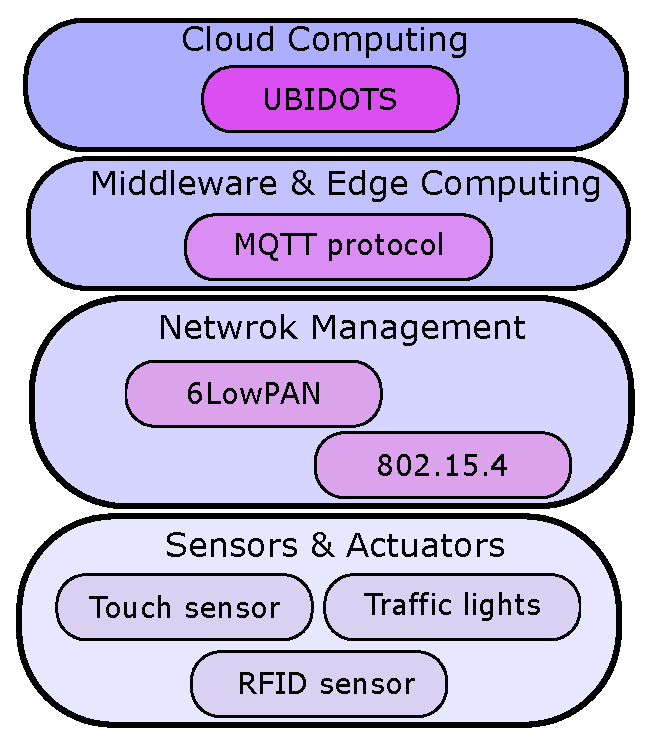
\includegraphics[width=2in]{Figures/StackIoTv1.eps}
\caption{UTLC network layers}
\label{fig:StackIoT.pdf}
\end{figure}

	\section{Results exploitation} \label{sec:Results exploitation}

% Initiation
%Below we report the results of applying the contagion process model to the Enron Email dataset.


% Final findings
%In summary,
%	results presented in this section show that if the trust coefficient between users is up to 0.8,
%	the vulnerability diffusion process through trust relationship is at its high level of speed.
%This what happens when a new information appears in a communication network and users forward it largely in the network.
%In addition,
%	this work gives a new insight to understand the relationship between trust,
%	reputation,
%	individual vulnerability and social vulnerability in the context of messaging services such as emails.


\subsection{Range}

\subsection{Response time}

\subsection{Connection speed}

\subsection{Power consumption}

	\section{Discussion} \label{sec:Conclusion}

%purpose
The purpose of the project was to find and examine a communication protocol that could be suitable for IoT applications,
	by investigating the current hardware,
	OS,
	and communication protocols and building a prototype from the selected choices.
What can be said about the investigation is that it is difficult to examine all candidates in detail;
	this means that a rough selection has to be made based on initial knowledge potentially discarding good options.
The general feeling is,
	however,
	that all of the examined candidates in this project were relevant and added valuable insights to the current technology status.
The assessment gave relevant and interesting results that improved the understanding in what IoT can be used for,
	and what further areas of investigation could be.
One of the most interesting areas of further investigation would be the RDC driver,
	as it directly affects the response time and thus also the connection speed.
Even though the power consumption was not in line with the expectations,
	the reason has been found and can be resolved.
Another conclusion is that IoT is not ready for real-time applications as the latency is much higher than expected,
	for the technologies assessed in this thesis,
	and also has a high spread.
As the latency increases for each subsequent network hop and the minimum observed latency per hop is 11ms,
	when using the always-on RDC,
	this type of communication will probably only be used for applications where response time can vary greatly,
	without affecting the functionality.
CoAP as a communication protocol shows a lot of promise when combined with 6LoWPAN and IEEE 802.15.4.
It performs well given its simplicity but has one disadvantage:
	the large overhead which comes from the MAC addressing fields in the IEEE 802.15.4 frame.
If this overhead could be reduced from the current 71\% to only 30%,
	the goodput would double.
A solution would be to use a similar mechanism as BLE where the packet size varies depending on application.
Each node also has computing time left as the MCU is more powerful  than needed for the given application;
	an improvement would be to use a less powerful MCU,
	like the ARM Cortex-M0+,
	to reduce the clock speed as suggested in the discussion.
When looking at the future-proof aspect the later suggestion is probably the better,
	as the clock then could be increased if more computing power is needed.
In the future,
	batteries will hopefully be able to store more energy,
	thus increasing the time between battery changes or reducing the battery size.


% \chapter[8:lk]{UTLC}
% 	\begin{abstract}

% Problem
Most traffic light's control systems in smart cities are wired and have a semi-static behavior.
They are time-based, with pre-configured pattern and expensive cameras.
% Existing solutions
Although traffic lights can communicate wirelessly with incoming vehicles,
	they are less adapted to an urban environment.
If we consider light signs as an Internet of Things (IoT) network,
	one issue is to model thoroughly the change of signs' states and the Quality of Service (QoS) of this network.
In this paper,
	we propose a new architecture of Urban Traffic Light Control based on an IoT network (IoT-UTLC).
The objective is to interconnect both roads' infrastructures and traffic lights through an IoT platform.
We designed our IoT-UTLC by selecting motes and protocols of wireless sensor network (WSN).
Message Queuing Telemetry Transport (MQTT) protocol has been integrated to manage QoS.
It enables lights to adapt remotely to any situation and smoothly interrupt traffic light's classic cycles.
Our experimental results show that the MQTT protocol is efficient when the packets rate exceeds 35\% of traffic flow,
	it reduces traffic delay up to 0.05s at 90\% of congestion.
After verification and validation of our solution using a UPPAAL model checker,
	our system has been prototyped.
Motes' functions have been implemented on Contiki OS and connected through a 6LoWPAN/IEEE 802.15.4 network.
Time-stamping messages have been performed throughout the system to evaluate the MQTT protocol with different QoS levels.
In our experiments,
	we measured the Round-trip delay time (RTT) of messages exchanged between the WSN and IoT Cloud.
The results show that MQTT decreases the RTT when the Cumulative Distributed Function (CDF) of generated messages exceeds 35\%.

\end{abstract}
% 	\section{Introduction} \label{sec:Introduction}




\subsection{Problem Statement}

\subsection{Background}

\subsection{Purpose (Goal)}

\subsection{Limitations}

\subsection{Method}


% The structure 
This paper is organized as follows.
Section \ref{sec:Related work} elucidates summary of related works.
% Section \ref{sec:Background} provide the required background.
In section \ref{sec:Approach}, we propose our ... to ....
Section \ref{sec:Experimentation} evaluates the performance of our ... in terms of packet delivery ratio,
	throughput,
	and power consumption.
% Our findings are presented in section \ref{sec:Results}.
Section \ref{sec:Conclusion} concludes the article and gives some ideas for future work.


% Needs by statistics: Context Current needs


% Problematic Current bad state of the research


%Challenges
The difficulty to build such system is 


%Contribution 
In this work we 

% The structure 
The article is organized as follows.
Section \ref{sec:Related work} elucidates summary of related works,
In section \ref{sec:Approach}, we propose our ... to ....
Section \ref{sec:Experimentation} evaluate the performance of our ... in terms of packet delivery ratio,
	throughput,
	and power consumption.
Section \ref{sec:Conclusions} concludes the article and gives some ideas for future work.





% 	\section{Related work} \label{Sec:Related_Works}

Petri nets (PNs) are widely used for traffic light modelling and control \cite{huang_modular_2014}.
In  \cite{difebbraro_trafficresponsive_2006},
	deterministic-timed Petri Nets have been used to describe signalized intersections.
Undesirable deadlock states might appear when the nets are tested for some use cases.
The authors in \cite{febbraro_using_2009} have modified PNs models including  stochastic-time for one single signalized intersection.
Dotoli and Fanti \cite{dotoli_urban_2004} have built a colored timed PN with a deterministic modular framework,
	in which parts of the system,
	and even parts of the subsystems,
	can be specified and analyzed separately.
Examples using modularity are given in Soares and Vrancken \cite{dossantossoares_modular_2012},
	in which a p-timed PN is used for the control of a traffic signal in both main road and side streets.
However,
	formal characteristics of PNs (\emph{e.g.},
	deadlock and liveliness) haven’t been discussed.
Moreover,
	PNs suffer from a lack of analysis and verification tools.
To overcome these limits of PNs,
	we propose UPPAAL timed automata for design and verification of coherent state of cross road's traffic light.
UPPAAL is a timed-based modelling software with a graphical user interface.
It is the result of the research works of two universities UPPsala University in Sweden (UPP) and AALborg University in Denmark (AAL) \cite{david_uppaal_2015}.

In \cite{Web0},
	thermal cameras and on-street wired sensors detect vehicles and pedestrians in order to adapt the cycle of traffic light control systems.
However,
	such a solution can be expensive.
In addition,
	the system uses only its local view of the environment to detect the arrival of a vehicle.
Other solutions use recent technologies such as wireless sensors devices to limit the cost of thermal cameras and reduce the time needed to deploy sensors.
In \cite{tlig_decentralized_2014} and \cite{rose_internet_2015},
	the authors propose an adaptive system based on local wireless communication between lights and vehicles.
But such a solution requires a global interconnection between all road's users and infrastructure.
This problem comes from the rigid definition of technologies' standards.
Our work is not only limited to establish WSN,
	but it is scalable to interconnect heterogeneous wireless technologies through the Internet.
The obtained WSN intends to meet multiple QoS requirements of IoT applying the MQTT protocol.
In \cite{Silva2018},
	the latency of MQTT has been evaluated by calculating the average round-trip delay between two clients located in two different continents.
However,
	the evaluation has been limited to the impact of messages' size.
In our work,
	we consider the period of generated messages,
	and we calculate the RTT delays from WSN to Cloud IoT plateform.

In \cite{huang_modular_2014} \cite{difebbraro_trafficresponsive_2006} \cite{febbraro_using_2009} \cite{dossantossoares_modular_2012},
	the authors focus only on the structural analysis of their models and the transitions between colors of traffic lights.
However,
	the implementation of their models as a service in the Internet of smart cities has not been discussed.
Moreover,
	their methodology is not tested with any real traffic lights' Testbed.

% 	\section{Background} \label{sec:Background}

% \subsubsection{Hardware}

% \subsubsection{Operating system}

% \subsubsection{Communication protocol}


% 	\section{Proposed Framework} \label{sec:Approach}


% A generic scheme to solve the configuration selection problem and any other similar selection problem is given in this section..
% The genetic selection scheme consists of three main steps,
% 	the first step contains a set of small parallel fuzzy logic (FL)-based subsystems,
% 	the second step is a multiple criteria decision making (MCDM) system,
% 	and the third step is a genetic algorithm (GA)-based component to assign a suitable weight for the criteria in the second component.
% The scheme decision phase can be described in more detail as follows.


% \begin{figure}
% \placetextbox{0.75}{0.8}{
% 		\tiny \mywhiteblackbox{
% 		\begin{tabular}{l} 
% 			Source program \\\hline
% 	        Ada\\
% 	        C/C++\\
% 	        Java\\ 
% 		    Perl\\
% 		    Python\\
% 		    ...
% 	    \end{tabular}
% 	}
% }
% \end{figure}


% \Figure{h}{.5}{drawing.svg}{kjkjkj rd}
	% \begin{tikzpicture}
	% 	\scriptsize
	% 	% \node[draw,align=left,dashed, text width = 0.2\linewidth] at (3,6) {Criteria c1 fuzzy based control};

	% 	\node[draw,align=left,dashed, text width = .5cm, text height = .5cm] at (3,6) {Multiple criteria decision making};
	% 	\node[draw,align=left,dashed, text width = 2cm, text height = 2cm] at (6,6) {Multiple criteria decision making};
	% 	\node[draw,align=left,dashed, text width = 2cm, text height = 2cm] at (6,3) {Genetic algorithm to determine weights of criteria (w1, ..., wn)};
	% 	\draw[->,black,thick,dashed] (0,0) -- (1,1);
	% \end{tikzpicture}

% \textbf{Definition:} stopping criteria, population size P, and mutation probability pm\\
% \textbf{Generate} randomly the initial configurations \\
% \textbf{repeat:}\\
% . . . \textbf{for} each configuration do\\
% . . . . . . Train a model \& compute configuration's fitness\\
% . . . \textbf{end}\\
% . . . \textbf{for} each reproduction 1 ... P/2 do\\
% . . . . . . \textbf{Select:} 2 configurations based on fitness\\
% . . . . . . \textbf{Crossover:} Produce 2 child configurations\\
% . . . . . . \textbf{Mutate:} child configurations with pm\\
% . . . \textbf{end}\\
% \textbf{until} stopping criterion are met\\

% \State\textbf{Definition:} stopping criteria, population size P, and mutation probability pm\\
% \State\textbf{Generate} randomly the initial configurations


\begin{algorithm}
	 \KwData{QoS constraints}
	 \KwResult{Ranked configuration list}



\SetKwFunction{FMain}{Main}
\SetKwProg{GA}{GA}{:}{end}
\GA{}{
	\Repeat{stopping criterion is met}{
		\For{each configuration}{
			Train \& compute configuration's fitness
		}
		\For{each reproduction 1 ... P/2}{
			\textbf{Select:} 2 configurations based on fitness\;
			\textbf{Crossover:} Produce 2 child configurations\;
			\textbf{Mutate:} child configurations with pm\;
		}
	}
}

% \SetKwFunction{FMain}{Main}
% \SetKwProg{FL}{FL}{:}{end}
% \FL{}{
%     \eIf{$error \geq e$}{
%         Do that as well
%     }{
%         Do otherwise
%     }
%     \While{$something \not= 0$ }{	
%         $var1 \leftarrow var2$  	
%     }

% }
% \eIf{understand}{
%   go to next section\;
%   current section becomes this one\;
% }{
%   go back to the beginning of current section\;
% }

\caption{LoRa Transmission Parameter Selection}
\end{algorithm}
\medskip

The scheme selection process can be described following these five steps:

\begin{enumerate}
	\item According to the Semtech SX1276 specification\cite{lorasemtech}, there is 6720 possible settings ($s_{1}$, ... ,$s_{6720}$) and the framework has to select the most optimal one or to rank them according to their relevance.
	\item The first step of the selection process depends on multiple criteria up to i ($c_{1}$, ... , $c_{i}$).
		Different type of criteria can be measured from different sources to cover the maximum point of views,
		as example,
		the network server requirements, the applications requirements and the devices conditions.
	\item The Fuzzy Logic (FL) based subsystem gives an initial score for each configuration that reflects its relevance.
		The different sets of scores ($d_{1}$, ... ,$d_{i}$) are sent to the \ac{MCDM} in the $5^{th}$ step.
	\item At the same time,
			the genetic algorithm (GA) \cite{alkhawlani_access_2008} assigns a suitable weight ($w_{1}$, ... ,$w_{i}$) for each initial selection decision according to the objective function that is required by the application.
			% according to the importance and sensitivities of ANS criteria to the different characteristics of a wireless heterogeneous environment.
	\item Using the initial scores coming from the $3^{rd}$ step and the weights that are assigned using the $4^{th}$ step,
			the multi criteria decision making{} \ac{MCDM} will select the most relevant settings and rank them according to their reward.
\end{enumerate}


\Figure{h}{1}{genetic}{The proposed scheme for LoRa transmission parameters selection based on \ac{GA}, \ac{FL} and \ac{MCDM}}

% 	\section{Prototyping} \label{sec:Experimentation}

% Intro
We have prototyped the wireless sensors and actuator's network of traffic lights and roads on a mockup \footnote{https://github.com/IoT-UTLC/Resources/wiki} of real intersection in Paris with a scale of 1:68.
Our specifications have been defined considering the low-cost and energy efficiency of the solution.
This Testbed is a proof of concept of not limited to our use case as it is scalable for other applications.
For example,
	additional sensors of fine particules could be implanted bringing correlation between traffic jam and pollution.

\begin{figure*}[!htb]
\centering
\includegraphics[width=4.5in]{Figures/ScenarioPaper.eps}
\caption{Architecture of  Iot-UTLC}
\label{fig:ScenarioPaper.eps}
\end{figure*}

Fig.
\ref{fig:ScenarioPaper.eps} shows the architecture of our IoT-UTLC with three layers.
From left to right,
	we have the WSN layer with connected traffic lights’ actuators,
	sensors and IEEE 802.15.4 transceivers.
The second part is the gateway of the WSN ensured by the BR and the Middleware \emph{i.e.} Python script launched by host computer.
The last layer is the Ubidots IoT Cloud Platform.
It is an open source solution used to collect and analyze WSN data.

\subsection{6LoWPAN, Contiki OS, Re-Mote and Border Router} \label{Sec:Contiki}

% 6LoWPAN
Our WSN is an IPv6 LowPower Wireless Personal Area Network (6LoWPAN) based on IEEE 802.15.4 stack.
It is well adapted to embedded wireless devices with energy aware constraint and for its capabilities to define a mesh topology.
Contiki Os\footnote{http://www.contiki-os.org/} has been used to implement networks' functions such as send,
	receive and data processing.
It is an embedded operating system with large open source community.
It supports Zolertia's Re-Motes \footnote{https://github.com/Zolertia/Resources/wiki/RE-Mote} and implements recent IEEE 802.15.4 standard specifications.
It also includes protocols such as RPL,
	CoAP and MQTT.
Furthermore,
	developer community is active and makes available source codes examples in order to help developing quickly new applications.

% Re-motes
Re-motes are compatible with our WSN specifications and our design model.
They are wireless devices with ultra-low power operation mode.
This choice has been motivated by long radio range of its IEEE 802.15.4 CC1200 transceiver,
	which transmits in the frequency band of 868-915 MHz.
In addition,
	each Re-Mote has analog and digital ports with a possibility to connect several analog sensors and actuators.
A Re-mote can be driven by a computer and become a sink and/or BR as well as a gateway between the 6LoWPAN network and the computer.

%\Figure{!htb}{1}{ethernetRouter.png}{Our Ethernet router}
\begin{figure}[!htb]
\centering
\includegraphics[width=2.5in]{Figures/ethernetRouter.png}
\caption{BR and sink combined on one board}
\label{fig:ethernetRouter.png}
\end{figure}

%[Explanation of how it works with the 2 radios,
To implement the previous model described in Section \ref{sec:Use Case and Model Design},
	we used six Re-motes:
	one for the BR,
	four to control the traffic lights and one Re-Mote to detect the arrival of a high priority vehicle near a crossing point.
For simplicity,
	we choose a touch sensor as a detecting device of priority vehicle.
We have developed four types of programs running on a Re-mote:
	traffic lights signs,
	sensors,
	high priority vehicle detecting device and BR function.
Sensors send periodically information to the IoT Cloud Platform with temperature,
	pressure or any relevant information that can be sensed.
As mentioned in the previous section,
	traffic lights are sub-divided into two modes:
	slaves and masters.
Masters nodes are the only ones to request the Middleware to change its light’s state and slaves simply change its state depending on received packets.
These roles are defined to reduce the overhead of network,
	redundancy and collisions,
	for instance.
Masters send periodically packets to request a change of state to the Middleware which forwards them to a Cloud platform.
 
BR node behaves differently compared to the other Re-motes.
The entries of its routing table are the list of Re-motes that pass through it.
It reroutes every packet it receives from its neighboring to host computer (or sink),
	which  creates a connection to the IoT Cloud platform.
Two options are possible to create our BR:
	i) separate the BR and sink and ii) combine both on the same device.
In our development,
	we worked on how to implement the sink and the BR nodes on the same Re-Mote board.
Fig.
\ref{fig:ethernetRouter.png} shows a prototype of the combined BR and sink,
	both connected to an ethernet interface.
Indeed,
	if the border router becomes an Ethernet router,
	there will no longer be any connection between the host/sink machine and the IoT Cloud platform.
Every Re-mote is able to connect independently to the IoT Cloud platform.
This approach has some advantages,
	such as the autonomy of the devices,
	but it generates an overhead requiring extra synchronization packets' exchange.
Therefore,
	we separate the sink and BR,
	since this solution is more flexible and resilient for our Testbed.

%The border router is at first a Re-mote,
%	but it has very different behavior and function.
%Indeed it has the task of re-routing every packet it receives from its cohorts to the serial port of the host machine.


%This machine will create a connection to the IoT Cloud platform and send the Re-motes messages to it and get responses for the Re-motes.
%The border router is a central node because it knows all to Re-motes in the 6LoWPAN which packets have transited by it.
%It acts as a Router and has a routing table of those Re-motes that pass through it.
%A web server page can be accessed to retrieve that information.
%We also tried a different approach of it.

 % [
%Transition with next paragraph => the use of MQTT to access the other "side" of the system
%Explanation of how it works (encapsulating the headers ...)
%]
%[
%Big part of how it works,
%what is good about it %New paragraph about the autonomous BR we were trying to develop
%Comparison between the 2 solutions
%]

% Autonomous BR
%As we have seen before,
%	this approach requires a Border Router linked the computer itself to the internet,
%	we tried to see if we can remove one part.
%Thus,
%	we added a component to the Re-mote in order to connect it directly to the internet via an Ethernet cable.

%[Transition with next paragraph => the use of MQTT to access the other "side" of the system]

\subsection{MQTT and UBIDOTS} \label{Sec:MQTT}

Fig.
\ref{fig:StackIoT.pdf} presents the layers of our UTLC network.
From bottom to up,
	the WSN network sense and/or detect,
	process and actuates traffic lights.
The second layer manages the 6 LowPan addressing and routing of packets throughout an IEEE 802.15.4 network.
The Edge Computing is the Middleware between the WSN and the Cloud platform.
For the setup of our UTLC,
	we start by establishing the access network of WSN.
The next step is to connect this network to Core network.
MQTT protocol controls three levels of QoS of exchanged packets from the WSN to the chosen Ubidots \footnote{https://ubidots.com/} Cloud platform.
It adopts IntServ approach for supporting quality of service in the network,
	it tags incoming packets in the border routers with different levels of priority.
Core routers read incoming packets headers and queue them according to their priority,
	packets with a high priority are sent faster compared to low priority ones.

MQTT ensures the QoS and publish/subscribe mechanisms through a broker.
The broker behaves as a server by filtering messages and organizing them in topics,
	which are strings used to filter messages and define the hierarchy of our data structure.
They allow us to organize how to receive multiple data from sensors such as temperature,
	up time,
	battery status and how to display them and obtain a real-time glance of our system.
It gets its messages from publishers and sends any modifications to entities,
	which that subscribed to the updated topics.
We used this mechanism with the Middleware in order to publish messages to the broker and get from the main topic the new values of the subscriber.

%We have seen in previous section what we used for our local sensors network, let's see now how we communicate with the IoT Cloud Platform. We will use MQTT which is a light-weight transportation protocol. In our solution, a python script will run an MQTT client to connect our WSN to Ubidots.

%MQTT ensures the QoS and publishes/subscribes mechanisms with a noteworthy topic organization. 

%The topics are strings used to filter messages and define the hierarchy of our data structure. They allow us to organize how to receive multiple data from sensors such as temperature, up time, battery status and how to display them and obtain a real-time glance of our system. 

%In addition, the broker behaves as a server by filtering messages and organize them in topics. It gets its messages from publishers and will send any modifications to entities which would have subscribed to the updated topics. We used this mechanism with the middleware in order to publish messages to the broker and get from the main topic the new values using the subscriber functionality.


The QoS feature of MQTT protocol manages network resources by handling retransmissions and guarantees the delivery of messages. It allows more control on messages by defining the level of guarantee. By default, the QoS is defined by three levels. The first one, level 0, is `At most one`. Level 1 is `At least one` where there is an acknowledgment to let the sender know that its packet has been received. Finally, level 2 `Exactly once` is the highest verification level with a request/response flows to ensure that only one message will be delivered and processed by the receiver. In our case, we applied levels 1 and 2 using \textit{paho.mqtt.client} Python library.  
%
%For example, subscribed clients could define the data QoS level of requested data by the source code shown bellow. 
For example, publisher of high priority data such as touch sensor has to indicate the highest level of QoS by the code shown bellow. 
We shared our implementation and its source codes at https://github.com/IoT-UTLC/contiki.
%
%\begin{footnotesize}
%\begin{lstlisting}
%# client receives a CONNACK response 
%# from the server.
%def on_connect(client, userdata, flags, rc):
%  print("Subscribed to " + MQTT_URL_TOPIC)
%  client.subscribe(MQTT_URL_TOPIC, 2) 
%  # 2nd arg is the QoS level to use 
%  # at maximum when it's needed
%\end{lstlisting}
%\end{footnotesize}

\begin{footnotesize}
\begin{lstlisting}
payload = json.dumps({"RoadA": data, "RoadB": 0})
res, mid = conn.publish(MQTT_URL_PUB, payload,
	  qos=int(QoS)) # QoS is QoS level to use 
\end{lstlisting}
\end{footnotesize}


%# The callback for when the client receives a CONNACK response from the server.
%def on_connect(client, userdata, flags, rc):
%	print("Connected with result code "+str(rc))
%	print("Subscribed to " + MQTT_URL_TOPIC)
%	client.subscribe(MQTT_URL_TOPIC, 2) 
                                                                                                                                                        
We experienced significant latency of high priority messages when we tested of IoT-UTLC mockup. Therefore, assessments of the MQTT protocol in our case provided significant information about its efficiency. 

%  For the end point the IoT Cloud platform,
% we wanted to be simple  %QoS and MQTT resilient by default (good implementation)
% Get relevant information from dashboard
% Access from anywhere (remote control possible)
% Structure our system / hierarchy
%
%As for the MQTT broker, we wanted an easy and powerful IoT Cloud Platform.
%It will be compatible with all technologies we chose for our prototyping,
%	so with an integration of MQTT and QoS levels.
%an IoT Cloud platform is a central point of the system as it keeps all the information about our WSN.
%Using the Cloud allows the system being accessible from anywhere on the internet.
%It is also a tool to filter and display relevant information in real-time from our system in the centralized dashboard.
%It can be possible to trigger some actions on the system via the dashboard.
%
%% Architecture
%Building this virtual infrastructure for this project has been challenging.
%we used MQTT topics mechanism to get the most of Ubidots to structure every data sent.
%We have a main topic which contains the states of the traffic light (RoadA and RoadB) in real time,
%	we created individual topics for every Re-mote acting as traffic lights or sensors.
%With this architecture,
%	we can have deep information on every device (such as its battery,
%	sensors data,
%	etc...).
%Moreover,
%	it could be scaled to match future needs.


%\Figure{!htb}{1}{cdf_distribution.pdf}{Normal,Gamma and Logistic distribution}
\begin{figure}[!htb]
\centering
\includegraphics[width=2in]{Figures/StackIoTv1.eps}
\caption{UTLC network layers}
\label{fig:StackIoT.pdf}
\end{figure}

% 	\section{Results exploitation} \label{sec:Results exploitation}

% Initiation
%Below we report the results of applying the contagion process model to the Enron Email dataset.


% Final findings
%In summary,
%	results presented in this section show that if the trust coefficient between users is up to 0.8,
%	the vulnerability diffusion process through trust relationship is at its high level of speed.
%This what happens when a new information appears in a communication network and users forward it largely in the network.
%In addition,
%	this work gives a new insight to understand the relationship between trust,
%	reputation,
%	individual vulnerability and social vulnerability in the context of messaging services such as emails.


\subsection{Range}

\subsection{Response time}

\subsection{Connection speed}

\subsection{Power consumption}

% 	\section{Discussion} \label{sec:Conclusion}

%purpose
The purpose of the project was to find and examine a communication protocol that could be suitable for IoT applications,
	by investigating the current hardware,
	OS,
	and communication protocols and building a prototype from the selected choices.
What can be said about the investigation is that it is difficult to examine all candidates in detail;
	this means that a rough selection has to be made based on initial knowledge potentially discarding good options.
The general feeling is,
	however,
	that all of the examined candidates in this project were relevant and added valuable insights to the current technology status.
The assessment gave relevant and interesting results that improved the understanding in what IoT can be used for,
	and what further areas of investigation could be.
One of the most interesting areas of further investigation would be the RDC driver,
	as it directly affects the response time and thus also the connection speed.
Even though the power consumption was not in line with the expectations,
	the reason has been found and can be resolved.
Another conclusion is that IoT is not ready for real-time applications as the latency is much higher than expected,
	for the technologies assessed in this thesis,
	and also has a high spread.
As the latency increases for each subsequent network hop and the minimum observed latency per hop is 11ms,
	when using the always-on RDC,
	this type of communication will probably only be used for applications where response time can vary greatly,
	without affecting the functionality.
CoAP as a communication protocol shows a lot of promise when combined with 6LoWPAN and IEEE 802.15.4.
It performs well given its simplicity but has one disadvantage:
	the large overhead which comes from the MAC addressing fields in the IEEE 802.15.4 frame.
If this overhead could be reduced from the current 71\% to only 30%,
	the goodput would double.
A solution would be to use a similar mechanism as BLE where the packet size varies depending on application.
Each node also has computing time left as the MCU is more powerful  than needed for the given application;
	an improvement would be to use a less powerful MCU,
	like the ARM Cortex-M0+,
	to reduce the clock speed as suggested in the discussion.
When looking at the future-proof aspect the later suggestion is probably the better,
	as the clock then could be increased if more computing power is needed.
In the future,
	batteries will hopefully be able to store more energy,
	thus increasing the time between battery changes or reducing the battery size.


\chapter[9:''Everything that has a beginning has an ending. Make your peace with that and all will be well'' - Jack Kornfield]{Conclusion}
	\input{9/0_conclusion}
\Appendix
% \chapter[B:''Dans tout conflit, découvrez celui qui se frotte les mains ... Vous verrez que ce n'est jamais celui qui se bagarre !''  - Marc Roussel]{Survey: IoT}
% 	\input{B/0_frame}
% 	\chapter{Application}
\begin{table}
\scriptsize
	\begin{tabulary}{\textwidth}{C|C|C|C|C|C|C|C}
		\textbf{Application protocol} & RestFull & Transport & Publish/Subscribe & Request/Response & Security & QoS & Header size (Byte)\\\hline
		\textbf{COAP}                 & \ok      & UDP       & \ok               & \ok              & DTLS     & \ok & 4           \\\hline
		\textbf{MQTT}                 & \ko      & TCP       & \ok               & \ko              & SSL      & \ok & 2           \\\hline
		\textbf{MQTT-SN}              & \ko      & TCP       & \ok               & \ko              & SSL      & \ok & 2           \\\hline
		\textbf{XMPP}                 & \ko      & TCP       & \ok               & \ok              & SSL      & \ko & -           \\\hline
		\textbf{AMQP}                 & \ko      & TCP       & \ok               & \ko              & SSL      & \ok & 8           \\\hline
		\textbf{DDS}                  & \ko      & UDP TCP   & \ok               & \ko              & SSL DTLS & \ok & -           \\\hline
		\textbf{HTTP}                 & \ok      & TCP       & \ko               & \ok              & SSL      & \ko & -           \\
	\end{tabulary}
	\caption{\label{tab:protocolsComparison} Application protocols comparison}
\end{table}

Smart systems in smart cities \cite{alba_intelligent_2016}
\begin{itemize}
	\item Smart Mobility
	\item Smart semaphores controle
	\item Smart Red Swarm
	\item Smart panels
	\item Smart bus scheduling
	\item Smart EV management
	\item Smart surface parking
	\item Smart signs
	\item Smart energy systems
	\item Smart lighting
	\item Smart water jet systems
	\item Smart residuals gathering
	\item Smart building construction
	\item Smart tourism
	\item Smart QRinfo
	\item Smart monitoring
	\item Smart hawkeye
\end{itemize}



\begin{table}[h!]
\scriptsize
	\begin{tabulary}{\textwidth}{L|C|C|C|C|C}
	Callenges-Applications  & Gids & EHealth & Transportations & Cities & \textbf{Building}\\\hline
	Ressources cinstraints  & +           & +++     & -               & ++           & +            \\\hline
	Mobility                & +           & ++      & +++             & +++          & -            \\\hline
	\textbf{Heterogeneity}  & ++          & ++      & ++              & +++          & +            \\\hline
	Scalability             & +++         & ++      & +++             & +++          & ++           \\\hline
	QoS cinstraints         & ++          & ++      & +++             & +++          & +++          \\\hline
	Data management         & ++          & +       & +++             & +++          & ++           \\\hline
	Lack of standardization & ++          & ++      & ++              & ++           & +++          \\\hline
	Amount of attacks       & +           & +       & +++             & +++          & +++          \\\hline
	Safety                  & ++          & ++      & +++             & ++           & +++          \\\hline
	\end{tabulary}
\caption{\label{tab:iot_challenges} Main IoT challenges\cite{kouicem_internet_2018}}
\end{table}

\begin{itemize}
	\item Network selection
	\begin{itemize}
		\item MADM
		\begin{itemize}
			\item Ranking methods
			\item Ranking \& weighted methods
		\end{itemize}
		\item Game theory
		\begin{itemize}
			\item Users vs users
			\item Users vs networks
			\item Networks vs network
		\end{itemize}
		\item Fuzzy logic
		\begin{itemize}
			\item as a score method
			\item another theory
		\end{itemize}
		\item Utility function
		\begin{itemize}
			\item 1
			\item 2
		\end{itemize}
	\end{itemize}
\end{itemize}



%\changefontsizes{5pt}
\begin{table}[h!]
\scriptsize
	\begin{tabulary}{\textwidth}{L|C|C|C|C|C|C|C|C|C}
	Paper           & Architecture & Availability & Reliability & Mobility & Performance & Management & Scalability & Interoperability & Security\\\hline
	IoT-A           &              &              &             &          &             &            &             &                  &         \\\hline
	IoT@Work        &              &              &             &          &             &            &             &                  &         \\\hline
	EBBITS          &              &              &             &          &             &            &             &                  &         \\\hline
	BETaas          &              &              &             &          &             &            &             &                  &         \\\hline
	CALIPSO         &              &              &             &          &             &            &             &                  &         \\\hline
	VITAL           &              &              &             &          &             &            &             &                  &         \\\hline
	SENSAI          &              &              &             &          &             &            &             &                  &         \\\hline
	RERUM           &              &              &             &          &             &            &             &                  &         \\\hline
	RELEYonIT       &              &              &             &          &             &            &             &                  &         \\\hline
	IoT6            &              &              &             &          &             &            &             &                  &         \\\hline
	OpenIoT         &              &              &             &          &             &            &             &                  &         \\\hline
	Apec IoV        &              &              &             &          &             &            &             &                  &         \\\hline
	Smart Santander &              &              &             &          &             &            &             &                  &         \\\hline
	OMA Device      &              &              &             &          &             &            &             &                  &         \\\hline
	OMA-DM          &              &              &             &          &             &            &             &                  &         \\\hline
	LWM2M           &              &              &             &          &             &            &             &                  &         \\\hline
	NETCONF Light   &              &              &             &          &             &            &             &                  &         \\\hline
	Kura            &              &              &             &          &             &            &             &                  &         \\\hline
	MASH            &              &              &             &          &             &            &             &                  &         \\\hline
	IoT-iCore       &              &              &             &          &             &            &             &                  &         \\\hline
	PROBE-IT        &              &              &             &          &             &            &             &                  &         \\\hline
	OpenIoT         &              &              &             &          &             &            &             &                  &         \\\hline
	LinkSmart       &              &              &             &          &             &            &             &                  &         \\\hline
	IETF SOLACE     &              &              &             &          &             &            &             &                  &         \\\hline
	BUTLER          &              &              &             &          &             &            &             &                  &         \\\hline
	Codo            &              &              &             &          &             &            &             &                  &         \\\hline
	SVELETE         &              &              &             &          &             &            &             &                  &         \\\hline
		\end{tabulary}
	\caption{\label{tab:Table54975} An example table.}
\end{table}


\begin{table}[h!]
\scriptsize
	\begin{tabulary}{\textwidth}{L|C|C|C|C}
	\bf{Platform}      & \ \bf{COAP} & \bf{XMPP} & \bf{MQTT}\\\hline
	\bf{Arkessa}       &             &           & \ok      \\\hline
	\bf{Axeda}         &             &           &          \\\hline
	\bf{Etherios}      &             &           &          \\\hline
	\bf{LittleBits}    &             &           &          \\\hline
	\bf{NanoService}   & \ok         &           &          \\\hline
	\bf{Nimbits}       &             & \ok       &          \\\hline
	\bf{Ninja blocks}  &             &           &          \\\hline
	\bf{OnePlateformv} & \ok         & \ok       &          \\\hline
	\bf{RealTime.io}   &             &           &          \\\hline
	\bf{SensorCloud}   &             &           &          \\\hline
	\bf{SmartThings}   &             &           &          \\\hline
	\bf{TempoDB}       &             &           &          \\\hline
	\bf{ThingWorx}     &             &           & \ok      \\\hline
	\bf{Xively}        &             &           & \ok      \\\hline
	\bf{Ubidots}       &             &           & \ok      \\\hline
	\end{tabulary}
	\caption{\label{tab:IoTPlatforms} IoT cloud platforms and their characteristics}
\end{table}



%%\changefontsizes{5pt}
\begin{table}[h!]
\scriptsize
	\begin{tabular}{l|l|l|l}
	\textbf{Use cases}         &  &  & \\\hline
	Health Monitoring          &  &  & \\\hline
	Water Distribution         &  &  & \\\hline
	Electricity Distribution   &  &  & \\\hline
	Smart Buildings            &  &  & \\\hline
	Intelligent Transportation &  &  & \\\hline
	Surveillance               &  &  & \\\hline
	Environmental Monitoring   &  &  & \\
	\end{tabular}
	\caption{\label{tab:IoTUseCase} Use cases \cite{hancke_role_2012}}
\end{table}



\begin{table}
\scriptsize
	\begin{tabulary}{\textwidth}{C|C|C|C|C|C|C|C}
		\textbf{Application protocol} & RestFull & Transport & Publish/Subscribe & Request/Response & Security & QoS & Header size (Byte)\\\hline
		\textbf{COAP}                 & \ok      & UDP       & \ok               & \ok              & DTLS     & \ok & 4           \\\hline
		\textbf{MQTT}                 & \ko      & TCP       & \ok               & \ko              & SSL      & \ok & 2           \\\hline
		\textbf{MQTT-SN}              & \ko      & TCP       & \ok               & \ko              & SSL      & \ok & 2           \\\hline
		\textbf{XMPP}                 & \ko      & TCP       & \ok               & \ok              & SSL      & \ko & -           \\\hline
		\textbf{AMQP}                 & \ko      & TCP       & \ok               & \ko              & SSL      & \ok & 8           \\\hline
		\textbf{DDS}                  & \ko      & UDP TCP   & \ok               & \ko              & SSL DTLS & \ok & -           \\\hline
		\textbf{HTTP}                 & \ok      & TCP       & \ko               & \ok              & SSL      & \ko & -           \\
	\end{tabulary}
	\caption{\label{tab:protocolsComparison} Application protocols comparison}
\end{table}











% 	\input{B/0_divers}
% 	\input{B/0_table}
% 	\onecolumn
\section{Papers}
\setlength{\hoffset}{-.5in}
\pagestyle{empty}




%\changefontsizes{6pt}
\begin{longtable}{lllllll}
	\bf{Characteristics}               & \bf{6LoWPAN}   & \bf{LoRaWAN}                    & \bf{SigFox}   & \bf{NB-IoT} & \textbf{INGENU} & \textbf{TELENSA}\\\hline
	\bf{Proprietary}                   &                &                                 & \ok           &             &                 &                 \\\hline
	\bf{Standar}                       & IETF           & LoRa Alliance                   &               & 3GPP        &                 &                 \\\hline
	\multirow{2}{*}{$\ac{CF}_{[MHz]}$} & 902-929        & 902-928                         & 902           &             &                 &                 \\
	\                                  & 868-868.6      & 863-870 and 434                 & 868           &             &                 &                 \\\hline
	\multirow{3}{*}{$\bf{Channels }$}  & 0016 for 2400  & 80             for 915          & 25            &             &                 &                 \\
	\                                  & 0010 for 915   & 10             for 868 and 780  &               &             &                 &                 \\
	\                                  & 0001 for 868.3 &                                 &               &             &                 &                 \\\hline
	\multirow{3}{*}{$\ac{BW}_{[MHz]}$} & 0005 for 2400  & 0.125 and 0.50 for 915          & 0.0001-0.0012 &             &                 &                 \\
	\                                  & 0002 for 915   & 0.125 and 0.25 for 868 and 780  &               &             &                 &                 \\
	\                                  & 0600 for 868.3 &                                 &               &             &                 &                 \\\hline
	\multirow{3}{*}{$\ac{DR}_{[kbps]}$}& 0250 for 2400  & 0.00098-0.0219 for 915          & 0.1-0.6       &             &                 &                 \\
	\                                  & 0040 for 915   & 0.250-0.05     for 868 and 780  &               &             &                 &                 \\
	\                                  & 0020 for 868.3 &                                 &               &             &                 &                 \\\hline
	\multirow{3}{*}{$\bf{Modulation}$} & QPSK for 2400  & LoRa           for 915          & BPSK and GFSK & QSPSK       &                 &                 \\
	\                                  & BPSK for 915   & LoRa and GFSK  for 868  and 780 &               &             &                 &                 \\
	\                                  & BPSK for 868.3 & \ac{CSS}                        &               &             &                 &                 \\
	\                                  &                & unslotted ALOHA                 &unslotted ALOHA&             & CDMA-like       &                 \\\hline
	\multirow{3}{*}{$\ac{CR}_{[dBm]}$} & -085 for 2400  & -137                            & -137          &             &                 &                 \\
	\                                  & -092 for 915   &                                 &               &             &                 &                 \\
	\                                  & -092 for 868.3 &                                 &               &             &                 &                 \\\hline
	Topology                           &                & Star, Stars                     & Star          &             & Star, Tree      & Star            \\\hline
	\ac{ADR}                           &                &       \ok                       & \ko           &             & \ok             & \ko             \\\hline
	\ac{PL}                            &                & <250B (depends on SF)           & 12B(UL),8B(DL)&             & 10KB            &                 \\\hline
	Handover                           &                & Multi \ac{BS}                   & Multi \ac{BS} &             &                 &                 \\\hline
	Security                           &                & AES 128b                        & \ko           &             & 16B hash, AES 256b&               \\\hline
	\ac{LS}                            &                & \ok                             & \ko           &             & \ko             & \ko             \\\hline
	\ac{FEC}                           &                & AES 128b                        & \ko           &             & \ok             & \ok             \\\hline
	\bf{Range}                         & 10-100 m       & 5-15 km                         & 10-50 km      & 1Km         &                 &                 \\\hline
	\bf{Battery lifetime}              & 1-2 years      & <10 years                       & <10 years     & <10 years   &                 &                 \\\hline
	\bf{Uplink}                        &                &                                 & 100bps        &             &                 &                 \\\hline
	\bf{Downlink}                      &                &                                 & 8 bytes/msg   &             &                 &                 \\\hline
	\bf{Cost}                          &                & 35e                             & 25e           & 1020e       &                 &                 \\\hline
	\bf{max msg/day}                   &                & Unlimited                       & 140(UL),4(DL) & Unlimited   &                 &                 \\\hline
	\bf{max Payload}                   &                & 243B                            & 12(UL),8(DL)  & 1600B       &                 &                 \\\hline
\caption{\label{tab:LPWan_characteristics} LPWan Characteristics \cite{al-kashoash_comparison_2016}}
\end{longtable}

\clearpage
\newpage
\setlength{\hoffset}{-0in}
\twocolumn
% \chapter[91:lk]{Social privacy score through vulnerability contagion process}
% 	\begin{abstract}

% Problem
Most traffic light's control systems in smart cities are wired and have a semi-static behavior.
They are time-based, with pre-configured pattern and expensive cameras.
% Existing solutions
Although traffic lights can communicate wirelessly with incoming vehicles,
	they are less adapted to an urban environment.
If we consider light signs as an Internet of Things (IoT) network,
	one issue is to model thoroughly the change of signs' states and the Quality of Service (QoS) of this network.
In this paper,
	we propose a new architecture of Urban Traffic Light Control based on an IoT network (IoT-UTLC).
The objective is to interconnect both roads' infrastructures and traffic lights through an IoT platform.
We designed our IoT-UTLC by selecting motes and protocols of wireless sensor network (WSN).
Message Queuing Telemetry Transport (MQTT) protocol has been integrated to manage QoS.
It enables lights to adapt remotely to any situation and smoothly interrupt traffic light's classic cycles.
Our experimental results show that the MQTT protocol is efficient when the packets rate exceeds 35\% of traffic flow,
	it reduces traffic delay up to 0.05s at 90\% of congestion.
After verification and validation of our solution using a UPPAAL model checker,
	our system has been prototyped.
Motes' functions have been implemented on Contiki OS and connected through a 6LoWPAN/IEEE 802.15.4 network.
Time-stamping messages have been performed throughout the system to evaluate the MQTT protocol with different QoS levels.
In our experiments,
	we measured the Round-trip delay time (RTT) of messages exchanged between the WSN and IoT Cloud.
The results show that MQTT decreases the RTT when the Cumulative Distributed Function (CDF) of generated messages exceeds 35\%.

\end{abstract}
% 	\section{Introduction} \label{sec:Introduction}




\subsection{Problem Statement}

\subsection{Background}

\subsection{Purpose (Goal)}

\subsection{Limitations}

\subsection{Method}


% The structure 
This paper is organized as follows.
Section \ref{sec:Related work} elucidates summary of related works.
% Section \ref{sec:Background} provide the required background.
In section \ref{sec:Approach}, we propose our ... to ....
Section \ref{sec:Experimentation} evaluates the performance of our ... in terms of packet delivery ratio,
	throughput,
	and power consumption.
% Our findings are presented in section \ref{sec:Results}.
Section \ref{sec:Conclusion} concludes the article and gives some ideas for future work.


% Needs by statistics: Context Current needs


% Problematic Current bad state of the research


%Challenges
The difficulty to build such system is 


%Contribution 
In this work we 

% The structure 
The article is organized as follows.
Section \ref{sec:Related work} elucidates summary of related works,
In section \ref{sec:Approach}, we propose our ... to ....
Section \ref{sec:Experimentation} evaluate the performance of our ... in terms of packet delivery ratio,
	throughput,
	and power consumption.
Section \ref{sec:Conclusions} concludes the article and gives some ideas for future work.





% 	\section{Related work} \label{Sec:Related_Works}

Petri nets (PNs) are widely used for traffic light modelling and control \cite{huang_modular_2014}.
In  \cite{difebbraro_trafficresponsive_2006},
	deterministic-timed Petri Nets have been used to describe signalized intersections.
Undesirable deadlock states might appear when the nets are tested for some use cases.
The authors in \cite{febbraro_using_2009} have modified PNs models including  stochastic-time for one single signalized intersection.
Dotoli and Fanti \cite{dotoli_urban_2004} have built a colored timed PN with a deterministic modular framework,
	in which parts of the system,
	and even parts of the subsystems,
	can be specified and analyzed separately.
Examples using modularity are given in Soares and Vrancken \cite{dossantossoares_modular_2012},
	in which a p-timed PN is used for the control of a traffic signal in both main road and side streets.
However,
	formal characteristics of PNs (\emph{e.g.},
	deadlock and liveliness) haven’t been discussed.
Moreover,
	PNs suffer from a lack of analysis and verification tools.
To overcome these limits of PNs,
	we propose UPPAAL timed automata for design and verification of coherent state of cross road's traffic light.
UPPAAL is a timed-based modelling software with a graphical user interface.
It is the result of the research works of two universities UPPsala University in Sweden (UPP) and AALborg University in Denmark (AAL) \cite{david_uppaal_2015}.

In \cite{Web0},
	thermal cameras and on-street wired sensors detect vehicles and pedestrians in order to adapt the cycle of traffic light control systems.
However,
	such a solution can be expensive.
In addition,
	the system uses only its local view of the environment to detect the arrival of a vehicle.
Other solutions use recent technologies such as wireless sensors devices to limit the cost of thermal cameras and reduce the time needed to deploy sensors.
In \cite{tlig_decentralized_2014} and \cite{rose_internet_2015},
	the authors propose an adaptive system based on local wireless communication between lights and vehicles.
But such a solution requires a global interconnection between all road's users and infrastructure.
This problem comes from the rigid definition of technologies' standards.
Our work is not only limited to establish WSN,
	but it is scalable to interconnect heterogeneous wireless technologies through the Internet.
The obtained WSN intends to meet multiple QoS requirements of IoT applying the MQTT protocol.
In \cite{Silva2018},
	the latency of MQTT has been evaluated by calculating the average round-trip delay between two clients located in two different continents.
However,
	the evaluation has been limited to the impact of messages' size.
In our work,
	we consider the period of generated messages,
	and we calculate the RTT delays from WSN to Cloud IoT plateform.

In \cite{huang_modular_2014} \cite{difebbraro_trafficresponsive_2006} \cite{febbraro_using_2009} \cite{dossantossoares_modular_2012},
	the authors focus only on the structural analysis of their models and the transitions between colors of traffic lights.
However,
	the implementation of their models as a service in the Internet of smart cities has not been discussed.
Moreover,
	their methodology is not tested with any real traffic lights' Testbed.

% 	\section{Background} \label{sec:Background}

% \subsubsection{Hardware}

% \subsubsection{Operating system}

% \subsubsection{Communication protocol}


% 	\section{Proposed Framework} \label{sec:Approach}


% A generic scheme to solve the configuration selection problem and any other similar selection problem is given in this section..
% The genetic selection scheme consists of three main steps,
% 	the first step contains a set of small parallel fuzzy logic (FL)-based subsystems,
% 	the second step is a multiple criteria decision making (MCDM) system,
% 	and the third step is a genetic algorithm (GA)-based component to assign a suitable weight for the criteria in the second component.
% The scheme decision phase can be described in more detail as follows.


% \begin{figure}
% \placetextbox{0.75}{0.8}{
% 		\tiny \mywhiteblackbox{
% 		\begin{tabular}{l} 
% 			Source program \\\hline
% 	        Ada\\
% 	        C/C++\\
% 	        Java\\ 
% 		    Perl\\
% 		    Python\\
% 		    ...
% 	    \end{tabular}
% 	}
% }
% \end{figure}


% \Figure{h}{.5}{drawing.svg}{kjkjkj rd}
	% \begin{tikzpicture}
	% 	\scriptsize
	% 	% \node[draw,align=left,dashed, text width = 0.2\linewidth] at (3,6) {Criteria c1 fuzzy based control};

	% 	\node[draw,align=left,dashed, text width = .5cm, text height = .5cm] at (3,6) {Multiple criteria decision making};
	% 	\node[draw,align=left,dashed, text width = 2cm, text height = 2cm] at (6,6) {Multiple criteria decision making};
	% 	\node[draw,align=left,dashed, text width = 2cm, text height = 2cm] at (6,3) {Genetic algorithm to determine weights of criteria (w1, ..., wn)};
	% 	\draw[->,black,thick,dashed] (0,0) -- (1,1);
	% \end{tikzpicture}

% \textbf{Definition:} stopping criteria, population size P, and mutation probability pm\\
% \textbf{Generate} randomly the initial configurations \\
% \textbf{repeat:}\\
% . . . \textbf{for} each configuration do\\
% . . . . . . Train a model \& compute configuration's fitness\\
% . . . \textbf{end}\\
% . . . \textbf{for} each reproduction 1 ... P/2 do\\
% . . . . . . \textbf{Select:} 2 configurations based on fitness\\
% . . . . . . \textbf{Crossover:} Produce 2 child configurations\\
% . . . . . . \textbf{Mutate:} child configurations with pm\\
% . . . \textbf{end}\\
% \textbf{until} stopping criterion are met\\

% \State\textbf{Definition:} stopping criteria, population size P, and mutation probability pm\\
% \State\textbf{Generate} randomly the initial configurations


\begin{algorithm}
	 \KwData{QoS constraints}
	 \KwResult{Ranked configuration list}



\SetKwFunction{FMain}{Main}
\SetKwProg{GA}{GA}{:}{end}
\GA{}{
	\Repeat{stopping criterion is met}{
		\For{each configuration}{
			Train \& compute configuration's fitness
		}
		\For{each reproduction 1 ... P/2}{
			\textbf{Select:} 2 configurations based on fitness\;
			\textbf{Crossover:} Produce 2 child configurations\;
			\textbf{Mutate:} child configurations with pm\;
		}
	}
}

% \SetKwFunction{FMain}{Main}
% \SetKwProg{FL}{FL}{:}{end}
% \FL{}{
%     \eIf{$error \geq e$}{
%         Do that as well
%     }{
%         Do otherwise
%     }
%     \While{$something \not= 0$ }{	
%         $var1 \leftarrow var2$  	
%     }

% }
% \eIf{understand}{
%   go to next section\;
%   current section becomes this one\;
% }{
%   go back to the beginning of current section\;
% }

\caption{LoRa Transmission Parameter Selection}
\end{algorithm}
\medskip

The scheme selection process can be described following these five steps:

\begin{enumerate}
	\item According to the Semtech SX1276 specification\cite{lorasemtech}, there is 6720 possible settings ($s_{1}$, ... ,$s_{6720}$) and the framework has to select the most optimal one or to rank them according to their relevance.
	\item The first step of the selection process depends on multiple criteria up to i ($c_{1}$, ... , $c_{i}$).
		Different type of criteria can be measured from different sources to cover the maximum point of views,
		as example,
		the network server requirements, the applications requirements and the devices conditions.
	\item The Fuzzy Logic (FL) based subsystem gives an initial score for each configuration that reflects its relevance.
		The different sets of scores ($d_{1}$, ... ,$d_{i}$) are sent to the \ac{MCDM} in the $5^{th}$ step.
	\item At the same time,
			the genetic algorithm (GA) \cite{alkhawlani_access_2008} assigns a suitable weight ($w_{1}$, ... ,$w_{i}$) for each initial selection decision according to the objective function that is required by the application.
			% according to the importance and sensitivities of ANS criteria to the different characteristics of a wireless heterogeneous environment.
	\item Using the initial scores coming from the $3^{rd}$ step and the weights that are assigned using the $4^{th}$ step,
			the multi criteria decision making{} \ac{MCDM} will select the most relevant settings and rank them according to their reward.
\end{enumerate}


\Figure{h}{1}{genetic}{The proposed scheme for LoRa transmission parameters selection based on \ac{GA}, \ac{FL} and \ac{MCDM}}

% 	\section{Prototyping} \label{sec:Experimentation}

% Intro
We have prototyped the wireless sensors and actuator's network of traffic lights and roads on a mockup \footnote{https://github.com/IoT-UTLC/Resources/wiki} of real intersection in Paris with a scale of 1:68.
Our specifications have been defined considering the low-cost and energy efficiency of the solution.
This Testbed is a proof of concept of not limited to our use case as it is scalable for other applications.
For example,
	additional sensors of fine particules could be implanted bringing correlation between traffic jam and pollution.

\begin{figure*}[!htb]
\centering
\includegraphics[width=4.5in]{Figures/ScenarioPaper.eps}
\caption{Architecture of  Iot-UTLC}
\label{fig:ScenarioPaper.eps}
\end{figure*}

Fig.
\ref{fig:ScenarioPaper.eps} shows the architecture of our IoT-UTLC with three layers.
From left to right,
	we have the WSN layer with connected traffic lights’ actuators,
	sensors and IEEE 802.15.4 transceivers.
The second part is the gateway of the WSN ensured by the BR and the Middleware \emph{i.e.} Python script launched by host computer.
The last layer is the Ubidots IoT Cloud Platform.
It is an open source solution used to collect and analyze WSN data.

\subsection{6LoWPAN, Contiki OS, Re-Mote and Border Router} \label{Sec:Contiki}

% 6LoWPAN
Our WSN is an IPv6 LowPower Wireless Personal Area Network (6LoWPAN) based on IEEE 802.15.4 stack.
It is well adapted to embedded wireless devices with energy aware constraint and for its capabilities to define a mesh topology.
Contiki Os\footnote{http://www.contiki-os.org/} has been used to implement networks' functions such as send,
	receive and data processing.
It is an embedded operating system with large open source community.
It supports Zolertia's Re-Motes \footnote{https://github.com/Zolertia/Resources/wiki/RE-Mote} and implements recent IEEE 802.15.4 standard specifications.
It also includes protocols such as RPL,
	CoAP and MQTT.
Furthermore,
	developer community is active and makes available source codes examples in order to help developing quickly new applications.

% Re-motes
Re-motes are compatible with our WSN specifications and our design model.
They are wireless devices with ultra-low power operation mode.
This choice has been motivated by long radio range of its IEEE 802.15.4 CC1200 transceiver,
	which transmits in the frequency band of 868-915 MHz.
In addition,
	each Re-Mote has analog and digital ports with a possibility to connect several analog sensors and actuators.
A Re-mote can be driven by a computer and become a sink and/or BR as well as a gateway between the 6LoWPAN network and the computer.

%\Figure{!htb}{1}{ethernetRouter.png}{Our Ethernet router}
\begin{figure}[!htb]
\centering
\includegraphics[width=2.5in]{Figures/ethernetRouter.png}
\caption{BR and sink combined on one board}
\label{fig:ethernetRouter.png}
\end{figure}

%[Explanation of how it works with the 2 radios,
To implement the previous model described in Section \ref{sec:Use Case and Model Design},
	we used six Re-motes:
	one for the BR,
	four to control the traffic lights and one Re-Mote to detect the arrival of a high priority vehicle near a crossing point.
For simplicity,
	we choose a touch sensor as a detecting device of priority vehicle.
We have developed four types of programs running on a Re-mote:
	traffic lights signs,
	sensors,
	high priority vehicle detecting device and BR function.
Sensors send periodically information to the IoT Cloud Platform with temperature,
	pressure or any relevant information that can be sensed.
As mentioned in the previous section,
	traffic lights are sub-divided into two modes:
	slaves and masters.
Masters nodes are the only ones to request the Middleware to change its light’s state and slaves simply change its state depending on received packets.
These roles are defined to reduce the overhead of network,
	redundancy and collisions,
	for instance.
Masters send periodically packets to request a change of state to the Middleware which forwards them to a Cloud platform.
 
BR node behaves differently compared to the other Re-motes.
The entries of its routing table are the list of Re-motes that pass through it.
It reroutes every packet it receives from its neighboring to host computer (or sink),
	which  creates a connection to the IoT Cloud platform.
Two options are possible to create our BR:
	i) separate the BR and sink and ii) combine both on the same device.
In our development,
	we worked on how to implement the sink and the BR nodes on the same Re-Mote board.
Fig.
\ref{fig:ethernetRouter.png} shows a prototype of the combined BR and sink,
	both connected to an ethernet interface.
Indeed,
	if the border router becomes an Ethernet router,
	there will no longer be any connection between the host/sink machine and the IoT Cloud platform.
Every Re-mote is able to connect independently to the IoT Cloud platform.
This approach has some advantages,
	such as the autonomy of the devices,
	but it generates an overhead requiring extra synchronization packets' exchange.
Therefore,
	we separate the sink and BR,
	since this solution is more flexible and resilient for our Testbed.

%The border router is at first a Re-mote,
%	but it has very different behavior and function.
%Indeed it has the task of re-routing every packet it receives from its cohorts to the serial port of the host machine.


%This machine will create a connection to the IoT Cloud platform and send the Re-motes messages to it and get responses for the Re-motes.
%The border router is a central node because it knows all to Re-motes in the 6LoWPAN which packets have transited by it.
%It acts as a Router and has a routing table of those Re-motes that pass through it.
%A web server page can be accessed to retrieve that information.
%We also tried a different approach of it.

 % [
%Transition with next paragraph => the use of MQTT to access the other "side" of the system
%Explanation of how it works (encapsulating the headers ...)
%]
%[
%Big part of how it works,
%what is good about it %New paragraph about the autonomous BR we were trying to develop
%Comparison between the 2 solutions
%]

% Autonomous BR
%As we have seen before,
%	this approach requires a Border Router linked the computer itself to the internet,
%	we tried to see if we can remove one part.
%Thus,
%	we added a component to the Re-mote in order to connect it directly to the internet via an Ethernet cable.

%[Transition with next paragraph => the use of MQTT to access the other "side" of the system]

\subsection{MQTT and UBIDOTS} \label{Sec:MQTT}

Fig.
\ref{fig:StackIoT.pdf} presents the layers of our UTLC network.
From bottom to up,
	the WSN network sense and/or detect,
	process and actuates traffic lights.
The second layer manages the 6 LowPan addressing and routing of packets throughout an IEEE 802.15.4 network.
The Edge Computing is the Middleware between the WSN and the Cloud platform.
For the setup of our UTLC,
	we start by establishing the access network of WSN.
The next step is to connect this network to Core network.
MQTT protocol controls three levels of QoS of exchanged packets from the WSN to the chosen Ubidots \footnote{https://ubidots.com/} Cloud platform.
It adopts IntServ approach for supporting quality of service in the network,
	it tags incoming packets in the border routers with different levels of priority.
Core routers read incoming packets headers and queue them according to their priority,
	packets with a high priority are sent faster compared to low priority ones.

MQTT ensures the QoS and publish/subscribe mechanisms through a broker.
The broker behaves as a server by filtering messages and organizing them in topics,
	which are strings used to filter messages and define the hierarchy of our data structure.
They allow us to organize how to receive multiple data from sensors such as temperature,
	up time,
	battery status and how to display them and obtain a real-time glance of our system.
It gets its messages from publishers and sends any modifications to entities,
	which that subscribed to the updated topics.
We used this mechanism with the Middleware in order to publish messages to the broker and get from the main topic the new values of the subscriber.

%We have seen in previous section what we used for our local sensors network, let's see now how we communicate with the IoT Cloud Platform. We will use MQTT which is a light-weight transportation protocol. In our solution, a python script will run an MQTT client to connect our WSN to Ubidots.

%MQTT ensures the QoS and publishes/subscribes mechanisms with a noteworthy topic organization. 

%The topics are strings used to filter messages and define the hierarchy of our data structure. They allow us to organize how to receive multiple data from sensors such as temperature, up time, battery status and how to display them and obtain a real-time glance of our system. 

%In addition, the broker behaves as a server by filtering messages and organize them in topics. It gets its messages from publishers and will send any modifications to entities which would have subscribed to the updated topics. We used this mechanism with the middleware in order to publish messages to the broker and get from the main topic the new values using the subscriber functionality.


The QoS feature of MQTT protocol manages network resources by handling retransmissions and guarantees the delivery of messages. It allows more control on messages by defining the level of guarantee. By default, the QoS is defined by three levels. The first one, level 0, is `At most one`. Level 1 is `At least one` where there is an acknowledgment to let the sender know that its packet has been received. Finally, level 2 `Exactly once` is the highest verification level with a request/response flows to ensure that only one message will be delivered and processed by the receiver. In our case, we applied levels 1 and 2 using \textit{paho.mqtt.client} Python library.  
%
%For example, subscribed clients could define the data QoS level of requested data by the source code shown bellow. 
For example, publisher of high priority data such as touch sensor has to indicate the highest level of QoS by the code shown bellow. 
We shared our implementation and its source codes at https://github.com/IoT-UTLC/contiki.
%
%\begin{footnotesize}
%\begin{lstlisting}
%# client receives a CONNACK response 
%# from the server.
%def on_connect(client, userdata, flags, rc):
%  print("Subscribed to " + MQTT_URL_TOPIC)
%  client.subscribe(MQTT_URL_TOPIC, 2) 
%  # 2nd arg is the QoS level to use 
%  # at maximum when it's needed
%\end{lstlisting}
%\end{footnotesize}

\begin{footnotesize}
\begin{lstlisting}
payload = json.dumps({"RoadA": data, "RoadB": 0})
res, mid = conn.publish(MQTT_URL_PUB, payload,
	  qos=int(QoS)) # QoS is QoS level to use 
\end{lstlisting}
\end{footnotesize}


%# The callback for when the client receives a CONNACK response from the server.
%def on_connect(client, userdata, flags, rc):
%	print("Connected with result code "+str(rc))
%	print("Subscribed to " + MQTT_URL_TOPIC)
%	client.subscribe(MQTT_URL_TOPIC, 2) 
                                                                                                                                                        
We experienced significant latency of high priority messages when we tested of IoT-UTLC mockup. Therefore, assessments of the MQTT protocol in our case provided significant information about its efficiency. 

%  For the end point the IoT Cloud platform,
% we wanted to be simple  %QoS and MQTT resilient by default (good implementation)
% Get relevant information from dashboard
% Access from anywhere (remote control possible)
% Structure our system / hierarchy
%
%As for the MQTT broker, we wanted an easy and powerful IoT Cloud Platform.
%It will be compatible with all technologies we chose for our prototyping,
%	so with an integration of MQTT and QoS levels.
%an IoT Cloud platform is a central point of the system as it keeps all the information about our WSN.
%Using the Cloud allows the system being accessible from anywhere on the internet.
%It is also a tool to filter and display relevant information in real-time from our system in the centralized dashboard.
%It can be possible to trigger some actions on the system via the dashboard.
%
%% Architecture
%Building this virtual infrastructure for this project has been challenging.
%we used MQTT topics mechanism to get the most of Ubidots to structure every data sent.
%We have a main topic which contains the states of the traffic light (RoadA and RoadB) in real time,
%	we created individual topics for every Re-mote acting as traffic lights or sensors.
%With this architecture,
%	we can have deep information on every device (such as its battery,
%	sensors data,
%	etc...).
%Moreover,
%	it could be scaled to match future needs.


%\Figure{!htb}{1}{cdf_distribution.pdf}{Normal,Gamma and Logistic distribution}
\begin{figure}[!htb]
\centering
\includegraphics[width=2in]{Figures/StackIoTv1.eps}
\caption{UTLC network layers}
\label{fig:StackIoT.pdf}
\end{figure}

% 	\section{Results exploitation} \label{sec:Results exploitation}

% Initiation
%Below we report the results of applying the contagion process model to the Enron Email dataset.


% Final findings
%In summary,
%	results presented in this section show that if the trust coefficient between users is up to 0.8,
%	the vulnerability diffusion process through trust relationship is at its high level of speed.
%This what happens when a new information appears in a communication network and users forward it largely in the network.
%In addition,
%	this work gives a new insight to understand the relationship between trust,
%	reputation,
%	individual vulnerability and social vulnerability in the context of messaging services such as emails.


\subsection{Range}

\subsection{Response time}

\subsection{Connection speed}

\subsection{Power consumption}

% 	\section{Discussion} \label{sec:Conclusion}

%purpose
The purpose of the project was to find and examine a communication protocol that could be suitable for IoT applications,
	by investigating the current hardware,
	OS,
	and communication protocols and building a prototype from the selected choices.
What can be said about the investigation is that it is difficult to examine all candidates in detail;
	this means that a rough selection has to be made based on initial knowledge potentially discarding good options.
The general feeling is,
	however,
	that all of the examined candidates in this project were relevant and added valuable insights to the current technology status.
The assessment gave relevant and interesting results that improved the understanding in what IoT can be used for,
	and what further areas of investigation could be.
One of the most interesting areas of further investigation would be the RDC driver,
	as it directly affects the response time and thus also the connection speed.
Even though the power consumption was not in line with the expectations,
	the reason has been found and can be resolved.
Another conclusion is that IoT is not ready for real-time applications as the latency is much higher than expected,
	for the technologies assessed in this thesis,
	and also has a high spread.
As the latency increases for each subsequent network hop and the minimum observed latency per hop is 11ms,
	when using the always-on RDC,
	this type of communication will probably only be used for applications where response time can vary greatly,
	without affecting the functionality.
CoAP as a communication protocol shows a lot of promise when combined with 6LoWPAN and IEEE 802.15.4.
It performs well given its simplicity but has one disadvantage:
	the large overhead which comes from the MAC addressing fields in the IEEE 802.15.4 frame.
If this overhead could be reduced from the current 71\% to only 30%,
	the goodput would double.
A solution would be to use a similar mechanism as BLE where the packet size varies depending on application.
Each node also has computing time left as the MCU is more powerful  than needed for the given application;
	an improvement would be to use a less powerful MCU,
	like the ARM Cortex-M0+,
	to reduce the clock speed as suggested in the discussion.
When looking at the future-proof aspect the later suggestion is probably the better,
	as the clock then could be increased if more computing power is needed.
In the future,
	batteries will hopefully be able to store more energy,
	thus increasing the time between battery changes or reducing the battery size.


% \chapter[92:lk]{Privacy Framework}
% 	\begin{abstract}

% Problem
Most traffic light's control systems in smart cities are wired and have a semi-static behavior.
They are time-based, with pre-configured pattern and expensive cameras.
% Existing solutions
Although traffic lights can communicate wirelessly with incoming vehicles,
	they are less adapted to an urban environment.
If we consider light signs as an Internet of Things (IoT) network,
	one issue is to model thoroughly the change of signs' states and the Quality of Service (QoS) of this network.
In this paper,
	we propose a new architecture of Urban Traffic Light Control based on an IoT network (IoT-UTLC).
The objective is to interconnect both roads' infrastructures and traffic lights through an IoT platform.
We designed our IoT-UTLC by selecting motes and protocols of wireless sensor network (WSN).
Message Queuing Telemetry Transport (MQTT) protocol has been integrated to manage QoS.
It enables lights to adapt remotely to any situation and smoothly interrupt traffic light's classic cycles.
Our experimental results show that the MQTT protocol is efficient when the packets rate exceeds 35\% of traffic flow,
	it reduces traffic delay up to 0.05s at 90\% of congestion.
After verification and validation of our solution using a UPPAAL model checker,
	our system has been prototyped.
Motes' functions have been implemented on Contiki OS and connected through a 6LoWPAN/IEEE 802.15.4 network.
Time-stamping messages have been performed throughout the system to evaluate the MQTT protocol with different QoS levels.
In our experiments,
	we measured the Round-trip delay time (RTT) of messages exchanged between the WSN and IoT Cloud.
The results show that MQTT decreases the RTT when the Cumulative Distributed Function (CDF) of generated messages exceeds 35\%.

\end{abstract}
% 	\section{Introduction} \label{sec:Introduction}




\subsection{Problem Statement}

\subsection{Background}

\subsection{Purpose (Goal)}

\subsection{Limitations}

\subsection{Method}


% The structure 
This paper is organized as follows.
Section \ref{sec:Related work} elucidates summary of related works.
% Section \ref{sec:Background} provide the required background.
In section \ref{sec:Approach}, we propose our ... to ....
Section \ref{sec:Experimentation} evaluates the performance of our ... in terms of packet delivery ratio,
	throughput,
	and power consumption.
% Our findings are presented in section \ref{sec:Results}.
Section \ref{sec:Conclusion} concludes the article and gives some ideas for future work.


% Needs by statistics: Context Current needs


% Problematic Current bad state of the research


%Challenges
The difficulty to build such system is 


%Contribution 
In this work we 

% The structure 
The article is organized as follows.
Section \ref{sec:Related work} elucidates summary of related works,
In section \ref{sec:Approach}, we propose our ... to ....
Section \ref{sec:Experimentation} evaluate the performance of our ... in terms of packet delivery ratio,
	throughput,
	and power consumption.
Section \ref{sec:Conclusions} concludes the article and gives some ideas for future work.





% 	\section{Related work} \label{Sec:Related_Works}

Petri nets (PNs) are widely used for traffic light modelling and control \cite{huang_modular_2014}.
In  \cite{difebbraro_trafficresponsive_2006},
	deterministic-timed Petri Nets have been used to describe signalized intersections.
Undesirable deadlock states might appear when the nets are tested for some use cases.
The authors in \cite{febbraro_using_2009} have modified PNs models including  stochastic-time for one single signalized intersection.
Dotoli and Fanti \cite{dotoli_urban_2004} have built a colored timed PN with a deterministic modular framework,
	in which parts of the system,
	and even parts of the subsystems,
	can be specified and analyzed separately.
Examples using modularity are given in Soares and Vrancken \cite{dossantossoares_modular_2012},
	in which a p-timed PN is used for the control of a traffic signal in both main road and side streets.
However,
	formal characteristics of PNs (\emph{e.g.},
	deadlock and liveliness) haven’t been discussed.
Moreover,
	PNs suffer from a lack of analysis and verification tools.
To overcome these limits of PNs,
	we propose UPPAAL timed automata for design and verification of coherent state of cross road's traffic light.
UPPAAL is a timed-based modelling software with a graphical user interface.
It is the result of the research works of two universities UPPsala University in Sweden (UPP) and AALborg University in Denmark (AAL) \cite{david_uppaal_2015}.

In \cite{Web0},
	thermal cameras and on-street wired sensors detect vehicles and pedestrians in order to adapt the cycle of traffic light control systems.
However,
	such a solution can be expensive.
In addition,
	the system uses only its local view of the environment to detect the arrival of a vehicle.
Other solutions use recent technologies such as wireless sensors devices to limit the cost of thermal cameras and reduce the time needed to deploy sensors.
In \cite{tlig_decentralized_2014} and \cite{rose_internet_2015},
	the authors propose an adaptive system based on local wireless communication between lights and vehicles.
But such a solution requires a global interconnection between all road's users and infrastructure.
This problem comes from the rigid definition of technologies' standards.
Our work is not only limited to establish WSN,
	but it is scalable to interconnect heterogeneous wireless technologies through the Internet.
The obtained WSN intends to meet multiple QoS requirements of IoT applying the MQTT protocol.
In \cite{Silva2018},
	the latency of MQTT has been evaluated by calculating the average round-trip delay between two clients located in two different continents.
However,
	the evaluation has been limited to the impact of messages' size.
In our work,
	we consider the period of generated messages,
	and we calculate the RTT delays from WSN to Cloud IoT plateform.

In \cite{huang_modular_2014} \cite{difebbraro_trafficresponsive_2006} \cite{febbraro_using_2009} \cite{dossantossoares_modular_2012},
	the authors focus only on the structural analysis of their models and the transitions between colors of traffic lights.
However,
	the implementation of their models as a service in the Internet of smart cities has not been discussed.
Moreover,
	their methodology is not tested with any real traffic lights' Testbed.

% 	\section{Background} \label{sec:Background}

% \subsubsection{Hardware}

% \subsubsection{Operating system}

% \subsubsection{Communication protocol}


% 	\section{Proposed Framework} \label{sec:Approach}


% A generic scheme to solve the configuration selection problem and any other similar selection problem is given in this section..
% The genetic selection scheme consists of three main steps,
% 	the first step contains a set of small parallel fuzzy logic (FL)-based subsystems,
% 	the second step is a multiple criteria decision making (MCDM) system,
% 	and the third step is a genetic algorithm (GA)-based component to assign a suitable weight for the criteria in the second component.
% The scheme decision phase can be described in more detail as follows.


% \begin{figure}
% \placetextbox{0.75}{0.8}{
% 		\tiny \mywhiteblackbox{
% 		\begin{tabular}{l} 
% 			Source program \\\hline
% 	        Ada\\
% 	        C/C++\\
% 	        Java\\ 
% 		    Perl\\
% 		    Python\\
% 		    ...
% 	    \end{tabular}
% 	}
% }
% \end{figure}


% \Figure{h}{.5}{drawing.svg}{kjkjkj rd}
	% \begin{tikzpicture}
	% 	\scriptsize
	% 	% \node[draw,align=left,dashed, text width = 0.2\linewidth] at (3,6) {Criteria c1 fuzzy based control};

	% 	\node[draw,align=left,dashed, text width = .5cm, text height = .5cm] at (3,6) {Multiple criteria decision making};
	% 	\node[draw,align=left,dashed, text width = 2cm, text height = 2cm] at (6,6) {Multiple criteria decision making};
	% 	\node[draw,align=left,dashed, text width = 2cm, text height = 2cm] at (6,3) {Genetic algorithm to determine weights of criteria (w1, ..., wn)};
	% 	\draw[->,black,thick,dashed] (0,0) -- (1,1);
	% \end{tikzpicture}

% \textbf{Definition:} stopping criteria, population size P, and mutation probability pm\\
% \textbf{Generate} randomly the initial configurations \\
% \textbf{repeat:}\\
% . . . \textbf{for} each configuration do\\
% . . . . . . Train a model \& compute configuration's fitness\\
% . . . \textbf{end}\\
% . . . \textbf{for} each reproduction 1 ... P/2 do\\
% . . . . . . \textbf{Select:} 2 configurations based on fitness\\
% . . . . . . \textbf{Crossover:} Produce 2 child configurations\\
% . . . . . . \textbf{Mutate:} child configurations with pm\\
% . . . \textbf{end}\\
% \textbf{until} stopping criterion are met\\

% \State\textbf{Definition:} stopping criteria, population size P, and mutation probability pm\\
% \State\textbf{Generate} randomly the initial configurations


\begin{algorithm}
	 \KwData{QoS constraints}
	 \KwResult{Ranked configuration list}



\SetKwFunction{FMain}{Main}
\SetKwProg{GA}{GA}{:}{end}
\GA{}{
	\Repeat{stopping criterion is met}{
		\For{each configuration}{
			Train \& compute configuration's fitness
		}
		\For{each reproduction 1 ... P/2}{
			\textbf{Select:} 2 configurations based on fitness\;
			\textbf{Crossover:} Produce 2 child configurations\;
			\textbf{Mutate:} child configurations with pm\;
		}
	}
}

% \SetKwFunction{FMain}{Main}
% \SetKwProg{FL}{FL}{:}{end}
% \FL{}{
%     \eIf{$error \geq e$}{
%         Do that as well
%     }{
%         Do otherwise
%     }
%     \While{$something \not= 0$ }{	
%         $var1 \leftarrow var2$  	
%     }

% }
% \eIf{understand}{
%   go to next section\;
%   current section becomes this one\;
% }{
%   go back to the beginning of current section\;
% }

\caption{LoRa Transmission Parameter Selection}
\end{algorithm}
\medskip

The scheme selection process can be described following these five steps:

\begin{enumerate}
	\item According to the Semtech SX1276 specification\cite{lorasemtech}, there is 6720 possible settings ($s_{1}$, ... ,$s_{6720}$) and the framework has to select the most optimal one or to rank them according to their relevance.
	\item The first step of the selection process depends on multiple criteria up to i ($c_{1}$, ... , $c_{i}$).
		Different type of criteria can be measured from different sources to cover the maximum point of views,
		as example,
		the network server requirements, the applications requirements and the devices conditions.
	\item The Fuzzy Logic (FL) based subsystem gives an initial score for each configuration that reflects its relevance.
		The different sets of scores ($d_{1}$, ... ,$d_{i}$) are sent to the \ac{MCDM} in the $5^{th}$ step.
	\item At the same time,
			the genetic algorithm (GA) \cite{alkhawlani_access_2008} assigns a suitable weight ($w_{1}$, ... ,$w_{i}$) for each initial selection decision according to the objective function that is required by the application.
			% according to the importance and sensitivities of ANS criteria to the different characteristics of a wireless heterogeneous environment.
	\item Using the initial scores coming from the $3^{rd}$ step and the weights that are assigned using the $4^{th}$ step,
			the multi criteria decision making{} \ac{MCDM} will select the most relevant settings and rank them according to their reward.
\end{enumerate}


\Figure{h}{1}{genetic}{The proposed scheme for LoRa transmission parameters selection based on \ac{GA}, \ac{FL} and \ac{MCDM}}

% 	\section{Prototyping} \label{sec:Experimentation}

% Intro
We have prototyped the wireless sensors and actuator's network of traffic lights and roads on a mockup \footnote{https://github.com/IoT-UTLC/Resources/wiki} of real intersection in Paris with a scale of 1:68.
Our specifications have been defined considering the low-cost and energy efficiency of the solution.
This Testbed is a proof of concept of not limited to our use case as it is scalable for other applications.
For example,
	additional sensors of fine particules could be implanted bringing correlation between traffic jam and pollution.

\begin{figure*}[!htb]
\centering
\includegraphics[width=4.5in]{Figures/ScenarioPaper.eps}
\caption{Architecture of  Iot-UTLC}
\label{fig:ScenarioPaper.eps}
\end{figure*}

Fig.
\ref{fig:ScenarioPaper.eps} shows the architecture of our IoT-UTLC with three layers.
From left to right,
	we have the WSN layer with connected traffic lights’ actuators,
	sensors and IEEE 802.15.4 transceivers.
The second part is the gateway of the WSN ensured by the BR and the Middleware \emph{i.e.} Python script launched by host computer.
The last layer is the Ubidots IoT Cloud Platform.
It is an open source solution used to collect and analyze WSN data.

\subsection{6LoWPAN, Contiki OS, Re-Mote and Border Router} \label{Sec:Contiki}

% 6LoWPAN
Our WSN is an IPv6 LowPower Wireless Personal Area Network (6LoWPAN) based on IEEE 802.15.4 stack.
It is well adapted to embedded wireless devices with energy aware constraint and for its capabilities to define a mesh topology.
Contiki Os\footnote{http://www.contiki-os.org/} has been used to implement networks' functions such as send,
	receive and data processing.
It is an embedded operating system with large open source community.
It supports Zolertia's Re-Motes \footnote{https://github.com/Zolertia/Resources/wiki/RE-Mote} and implements recent IEEE 802.15.4 standard specifications.
It also includes protocols such as RPL,
	CoAP and MQTT.
Furthermore,
	developer community is active and makes available source codes examples in order to help developing quickly new applications.

% Re-motes
Re-motes are compatible with our WSN specifications and our design model.
They are wireless devices with ultra-low power operation mode.
This choice has been motivated by long radio range of its IEEE 802.15.4 CC1200 transceiver,
	which transmits in the frequency band of 868-915 MHz.
In addition,
	each Re-Mote has analog and digital ports with a possibility to connect several analog sensors and actuators.
A Re-mote can be driven by a computer and become a sink and/or BR as well as a gateway between the 6LoWPAN network and the computer.

%\Figure{!htb}{1}{ethernetRouter.png}{Our Ethernet router}
\begin{figure}[!htb]
\centering
\includegraphics[width=2.5in]{Figures/ethernetRouter.png}
\caption{BR and sink combined on one board}
\label{fig:ethernetRouter.png}
\end{figure}

%[Explanation of how it works with the 2 radios,
To implement the previous model described in Section \ref{sec:Use Case and Model Design},
	we used six Re-motes:
	one for the BR,
	four to control the traffic lights and one Re-Mote to detect the arrival of a high priority vehicle near a crossing point.
For simplicity,
	we choose a touch sensor as a detecting device of priority vehicle.
We have developed four types of programs running on a Re-mote:
	traffic lights signs,
	sensors,
	high priority vehicle detecting device and BR function.
Sensors send periodically information to the IoT Cloud Platform with temperature,
	pressure or any relevant information that can be sensed.
As mentioned in the previous section,
	traffic lights are sub-divided into two modes:
	slaves and masters.
Masters nodes are the only ones to request the Middleware to change its light’s state and slaves simply change its state depending on received packets.
These roles are defined to reduce the overhead of network,
	redundancy and collisions,
	for instance.
Masters send periodically packets to request a change of state to the Middleware which forwards them to a Cloud platform.
 
BR node behaves differently compared to the other Re-motes.
The entries of its routing table are the list of Re-motes that pass through it.
It reroutes every packet it receives from its neighboring to host computer (or sink),
	which  creates a connection to the IoT Cloud platform.
Two options are possible to create our BR:
	i) separate the BR and sink and ii) combine both on the same device.
In our development,
	we worked on how to implement the sink and the BR nodes on the same Re-Mote board.
Fig.
\ref{fig:ethernetRouter.png} shows a prototype of the combined BR and sink,
	both connected to an ethernet interface.
Indeed,
	if the border router becomes an Ethernet router,
	there will no longer be any connection between the host/sink machine and the IoT Cloud platform.
Every Re-mote is able to connect independently to the IoT Cloud platform.
This approach has some advantages,
	such as the autonomy of the devices,
	but it generates an overhead requiring extra synchronization packets' exchange.
Therefore,
	we separate the sink and BR,
	since this solution is more flexible and resilient for our Testbed.

%The border router is at first a Re-mote,
%	but it has very different behavior and function.
%Indeed it has the task of re-routing every packet it receives from its cohorts to the serial port of the host machine.


%This machine will create a connection to the IoT Cloud platform and send the Re-motes messages to it and get responses for the Re-motes.
%The border router is a central node because it knows all to Re-motes in the 6LoWPAN which packets have transited by it.
%It acts as a Router and has a routing table of those Re-motes that pass through it.
%A web server page can be accessed to retrieve that information.
%We also tried a different approach of it.

 % [
%Transition with next paragraph => the use of MQTT to access the other "side" of the system
%Explanation of how it works (encapsulating the headers ...)
%]
%[
%Big part of how it works,
%what is good about it %New paragraph about the autonomous BR we were trying to develop
%Comparison between the 2 solutions
%]

% Autonomous BR
%As we have seen before,
%	this approach requires a Border Router linked the computer itself to the internet,
%	we tried to see if we can remove one part.
%Thus,
%	we added a component to the Re-mote in order to connect it directly to the internet via an Ethernet cable.

%[Transition with next paragraph => the use of MQTT to access the other "side" of the system]

\subsection{MQTT and UBIDOTS} \label{Sec:MQTT}

Fig.
\ref{fig:StackIoT.pdf} presents the layers of our UTLC network.
From bottom to up,
	the WSN network sense and/or detect,
	process and actuates traffic lights.
The second layer manages the 6 LowPan addressing and routing of packets throughout an IEEE 802.15.4 network.
The Edge Computing is the Middleware between the WSN and the Cloud platform.
For the setup of our UTLC,
	we start by establishing the access network of WSN.
The next step is to connect this network to Core network.
MQTT protocol controls three levels of QoS of exchanged packets from the WSN to the chosen Ubidots \footnote{https://ubidots.com/} Cloud platform.
It adopts IntServ approach for supporting quality of service in the network,
	it tags incoming packets in the border routers with different levels of priority.
Core routers read incoming packets headers and queue them according to their priority,
	packets with a high priority are sent faster compared to low priority ones.

MQTT ensures the QoS and publish/subscribe mechanisms through a broker.
The broker behaves as a server by filtering messages and organizing them in topics,
	which are strings used to filter messages and define the hierarchy of our data structure.
They allow us to organize how to receive multiple data from sensors such as temperature,
	up time,
	battery status and how to display them and obtain a real-time glance of our system.
It gets its messages from publishers and sends any modifications to entities,
	which that subscribed to the updated topics.
We used this mechanism with the Middleware in order to publish messages to the broker and get from the main topic the new values of the subscriber.

%We have seen in previous section what we used for our local sensors network, let's see now how we communicate with the IoT Cloud Platform. We will use MQTT which is a light-weight transportation protocol. In our solution, a python script will run an MQTT client to connect our WSN to Ubidots.

%MQTT ensures the QoS and publishes/subscribes mechanisms with a noteworthy topic organization. 

%The topics are strings used to filter messages and define the hierarchy of our data structure. They allow us to organize how to receive multiple data from sensors such as temperature, up time, battery status and how to display them and obtain a real-time glance of our system. 

%In addition, the broker behaves as a server by filtering messages and organize them in topics. It gets its messages from publishers and will send any modifications to entities which would have subscribed to the updated topics. We used this mechanism with the middleware in order to publish messages to the broker and get from the main topic the new values using the subscriber functionality.


The QoS feature of MQTT protocol manages network resources by handling retransmissions and guarantees the delivery of messages. It allows more control on messages by defining the level of guarantee. By default, the QoS is defined by three levels. The first one, level 0, is `At most one`. Level 1 is `At least one` where there is an acknowledgment to let the sender know that its packet has been received. Finally, level 2 `Exactly once` is the highest verification level with a request/response flows to ensure that only one message will be delivered and processed by the receiver. In our case, we applied levels 1 and 2 using \textit{paho.mqtt.client} Python library.  
%
%For example, subscribed clients could define the data QoS level of requested data by the source code shown bellow. 
For example, publisher of high priority data such as touch sensor has to indicate the highest level of QoS by the code shown bellow. 
We shared our implementation and its source codes at https://github.com/IoT-UTLC/contiki.
%
%\begin{footnotesize}
%\begin{lstlisting}
%# client receives a CONNACK response 
%# from the server.
%def on_connect(client, userdata, flags, rc):
%  print("Subscribed to " + MQTT_URL_TOPIC)
%  client.subscribe(MQTT_URL_TOPIC, 2) 
%  # 2nd arg is the QoS level to use 
%  # at maximum when it's needed
%\end{lstlisting}
%\end{footnotesize}

\begin{footnotesize}
\begin{lstlisting}
payload = json.dumps({"RoadA": data, "RoadB": 0})
res, mid = conn.publish(MQTT_URL_PUB, payload,
	  qos=int(QoS)) # QoS is QoS level to use 
\end{lstlisting}
\end{footnotesize}


%# The callback for when the client receives a CONNACK response from the server.
%def on_connect(client, userdata, flags, rc):
%	print("Connected with result code "+str(rc))
%	print("Subscribed to " + MQTT_URL_TOPIC)
%	client.subscribe(MQTT_URL_TOPIC, 2) 
                                                                                                                                                        
We experienced significant latency of high priority messages when we tested of IoT-UTLC mockup. Therefore, assessments of the MQTT protocol in our case provided significant information about its efficiency. 

%  For the end point the IoT Cloud platform,
% we wanted to be simple  %QoS and MQTT resilient by default (good implementation)
% Get relevant information from dashboard
% Access from anywhere (remote control possible)
% Structure our system / hierarchy
%
%As for the MQTT broker, we wanted an easy and powerful IoT Cloud Platform.
%It will be compatible with all technologies we chose for our prototyping,
%	so with an integration of MQTT and QoS levels.
%an IoT Cloud platform is a central point of the system as it keeps all the information about our WSN.
%Using the Cloud allows the system being accessible from anywhere on the internet.
%It is also a tool to filter and display relevant information in real-time from our system in the centralized dashboard.
%It can be possible to trigger some actions on the system via the dashboard.
%
%% Architecture
%Building this virtual infrastructure for this project has been challenging.
%we used MQTT topics mechanism to get the most of Ubidots to structure every data sent.
%We have a main topic which contains the states of the traffic light (RoadA and RoadB) in real time,
%	we created individual topics for every Re-mote acting as traffic lights or sensors.
%With this architecture,
%	we can have deep information on every device (such as its battery,
%	sensors data,
%	etc...).
%Moreover,
%	it could be scaled to match future needs.


%\Figure{!htb}{1}{cdf_distribution.pdf}{Normal,Gamma and Logistic distribution}
\begin{figure}[!htb]
\centering
\includegraphics[width=2in]{Figures/StackIoTv1.eps}
\caption{UTLC network layers}
\label{fig:StackIoT.pdf}
\end{figure}

% 	\section{Results exploitation} \label{sec:Results exploitation}

% Initiation
%Below we report the results of applying the contagion process model to the Enron Email dataset.


% Final findings
%In summary,
%	results presented in this section show that if the trust coefficient between users is up to 0.8,
%	the vulnerability diffusion process through trust relationship is at its high level of speed.
%This what happens when a new information appears in a communication network and users forward it largely in the network.
%In addition,
%	this work gives a new insight to understand the relationship between trust,
%	reputation,
%	individual vulnerability and social vulnerability in the context of messaging services such as emails.


\subsection{Range}

\subsection{Response time}

\subsection{Connection speed}

\subsection{Power consumption}

% 	\section{Discussion} \label{sec:Conclusion}

%purpose
The purpose of the project was to find and examine a communication protocol that could be suitable for IoT applications,
	by investigating the current hardware,
	OS,
	and communication protocols and building a prototype from the selected choices.
What can be said about the investigation is that it is difficult to examine all candidates in detail;
	this means that a rough selection has to be made based on initial knowledge potentially discarding good options.
The general feeling is,
	however,
	that all of the examined candidates in this project were relevant and added valuable insights to the current technology status.
The assessment gave relevant and interesting results that improved the understanding in what IoT can be used for,
	and what further areas of investigation could be.
One of the most interesting areas of further investigation would be the RDC driver,
	as it directly affects the response time and thus also the connection speed.
Even though the power consumption was not in line with the expectations,
	the reason has been found and can be resolved.
Another conclusion is that IoT is not ready for real-time applications as the latency is much higher than expected,
	for the technologies assessed in this thesis,
	and also has a high spread.
As the latency increases for each subsequent network hop and the minimum observed latency per hop is 11ms,
	when using the always-on RDC,
	this type of communication will probably only be used for applications where response time can vary greatly,
	without affecting the functionality.
CoAP as a communication protocol shows a lot of promise when combined with 6LoWPAN and IEEE 802.15.4.
It performs well given its simplicity but has one disadvantage:
	the large overhead which comes from the MAC addressing fields in the IEEE 802.15.4 frame.
If this overhead could be reduced from the current 71\% to only 30%,
	the goodput would double.
A solution would be to use a similar mechanism as BLE where the packet size varies depending on application.
Each node also has computing time left as the MCU is more powerful  than needed for the given application;
	an improvement would be to use a less powerful MCU,
	like the ARM Cortex-M0+,
	to reduce the clock speed as suggested in the discussion.
When looking at the future-proof aspect the later suggestion is probably the better,
	as the clock then could be increased if more computing power is needed.
In the future,
	batteries will hopefully be able to store more energy,
	thus increasing the time between battery changes or reducing the battery size.


% \chapter[93:lk]{Survey: Privacy}
% 	\begin{abstract}

% Problem
Most traffic light's control systems in smart cities are wired and have a semi-static behavior.
They are time-based, with pre-configured pattern and expensive cameras.
% Existing solutions
Although traffic lights can communicate wirelessly with incoming vehicles,
	they are less adapted to an urban environment.
If we consider light signs as an Internet of Things (IoT) network,
	one issue is to model thoroughly the change of signs' states and the Quality of Service (QoS) of this network.
In this paper,
	we propose a new architecture of Urban Traffic Light Control based on an IoT network (IoT-UTLC).
The objective is to interconnect both roads' infrastructures and traffic lights through an IoT platform.
We designed our IoT-UTLC by selecting motes and protocols of wireless sensor network (WSN).
Message Queuing Telemetry Transport (MQTT) protocol has been integrated to manage QoS.
It enables lights to adapt remotely to any situation and smoothly interrupt traffic light's classic cycles.
Our experimental results show that the MQTT protocol is efficient when the packets rate exceeds 35\% of traffic flow,
	it reduces traffic delay up to 0.05s at 90\% of congestion.
After verification and validation of our solution using a UPPAAL model checker,
	our system has been prototyped.
Motes' functions have been implemented on Contiki OS and connected through a 6LoWPAN/IEEE 802.15.4 network.
Time-stamping messages have been performed throughout the system to evaluate the MQTT protocol with different QoS levels.
In our experiments,
	we measured the Round-trip delay time (RTT) of messages exchanged between the WSN and IoT Cloud.
The results show that MQTT decreases the RTT when the Cumulative Distributed Function (CDF) of generated messages exceeds 35\%.

\end{abstract}
% 	\section{Introduction} \label{sec:Introduction}




\subsection{Problem Statement}

\subsection{Background}

\subsection{Purpose (Goal)}

\subsection{Limitations}

\subsection{Method}


% The structure 
This paper is organized as follows.
Section \ref{sec:Related work} elucidates summary of related works.
% Section \ref{sec:Background} provide the required background.
In section \ref{sec:Approach}, we propose our ... to ....
Section \ref{sec:Experimentation} evaluates the performance of our ... in terms of packet delivery ratio,
	throughput,
	and power consumption.
% Our findings are presented in section \ref{sec:Results}.
Section \ref{sec:Conclusion} concludes the article and gives some ideas for future work.


% Needs by statistics: Context Current needs


% Problematic Current bad state of the research


%Challenges
The difficulty to build such system is 


%Contribution 
In this work we 

% The structure 
The article is organized as follows.
Section \ref{sec:Related work} elucidates summary of related works,
In section \ref{sec:Approach}, we propose our ... to ....
Section \ref{sec:Experimentation} evaluate the performance of our ... in terms of packet delivery ratio,
	throughput,
	and power consumption.
Section \ref{sec:Conclusions} concludes the article and gives some ideas for future work.





% 	\input{93/02_1_behavioral}
% 	\input{93/02_2_social}
% 	\input{93/02_3_technical}
% 	\section{Background} \label{sec:Background}

% \subsubsection{Hardware}

% \subsubsection{Operating system}

% \subsubsection{Communication protocol}


% 	\section{Discussion} \label{sec:Conclusion}

%purpose
The purpose of the project was to find and examine a communication protocol that could be suitable for IoT applications,
	by investigating the current hardware,
	OS,
	and communication protocols and building a prototype from the selected choices.
What can be said about the investigation is that it is difficult to examine all candidates in detail;
	this means that a rough selection has to be made based on initial knowledge potentially discarding good options.
The general feeling is,
	however,
	that all of the examined candidates in this project were relevant and added valuable insights to the current technology status.
The assessment gave relevant and interesting results that improved the understanding in what IoT can be used for,
	and what further areas of investigation could be.
One of the most interesting areas of further investigation would be the RDC driver,
	as it directly affects the response time and thus also the connection speed.
Even though the power consumption was not in line with the expectations,
	the reason has been found and can be resolved.
Another conclusion is that IoT is not ready for real-time applications as the latency is much higher than expected,
	for the technologies assessed in this thesis,
	and also has a high spread.
As the latency increases for each subsequent network hop and the minimum observed latency per hop is 11ms,
	when using the always-on RDC,
	this type of communication will probably only be used for applications where response time can vary greatly,
	without affecting the functionality.
CoAP as a communication protocol shows a lot of promise when combined with 6LoWPAN and IEEE 802.15.4.
It performs well given its simplicity but has one disadvantage:
	the large overhead which comes from the MAC addressing fields in the IEEE 802.15.4 frame.
If this overhead could be reduced from the current 71\% to only 30%,
	the goodput would double.
A solution would be to use a similar mechanism as BLE where the packet size varies depending on application.
Each node also has computing time left as the MCU is more powerful  than needed for the given application;
	an improvement would be to use a less powerful MCU,
	like the ARM Cortex-M0+,
	to reduce the clock speed as suggested in the discussion.
When looking at the future-proof aspect the later suggestion is probably the better,
	as the clock then could be increased if more computing power is needed.
In the future,
	batteries will hopefully be able to store more energy,
	thus increasing the time between battery changes or reducing the battery size.


% 	\input{93/0table}
\printbib
\end{refsection}
\end{document}
